\documentclass[12pt,twoside,dvipsnames]{article}
\usepackage{lscape}
\usepackage[small,bf]{caption}
\usepackage[charter]{mathdesign}
\usepackage{amsmath}
\usepackage{graphicx}
\usepackage{qtree}
\usepackage{subcaption}
\usepackage{fancyhdr}
%\usepackage{amsthm}
\usepackage{bm}
\usepackage{float}
\usepackage{cite}
\usepackage{pdflscape}
\usepackage{placeins}
\usepackage{afterpage}
\usepackage[hidelinks]{hyperref}
\usepackage{enumitem}
\usepackage{wrapfig}
\usepackage{multicol}
\usepackage{pdflscape}
%\usepackage{pdfpages}
\usepackage{layout}
\setlength{\headheight}{35pt}
\usepackage{longtable,booktabs}
\usepackage{makecell}

\DeclareMathOperator{\TE}{Total\ Error}
\DeclareMathOperator{\ME}{Measurement\ Error}
\DeclareMathOperator{\SE}{Sampling\ Error}
\DeclareMathOperator{\NE}{Nonresponse\ Error}
\DeclareMathOperator{\CE}{Coverage\ Error}
\DeclareMathOperator{\Bias}{Bias}
\DeclareMathOperator{\MSE}{MSE}
\DeclareMathOperator{\GE}{E}
\DeclareMathOperator{\GV}{V}
\DeclareMathOperator{\GC}{Cov}
\DeclareMathOperator{\SRS}{SRS}
\DeclareMathOperator{\StS}{StS}
\DeclareMathOperator{\SyS}{SyS}
\DeclareMathOperator{\ClS}{ClS}
\DeclareMathOperator{\PPS}{PPS}
\DeclareMathOperator{\MMS}{MMS}
\DeclareMathOperator{\MPS}{MPS}


\newtheorem{theorem}{Theorem}

\newcommand{\thedraft}{(DRAFT)}
%\newcommand{\thedraft}{}


\newcommand{\newtitle}{Introduction to Quantitative Consulting}

\voffset=-.5in
\hoffset=-.75in
\oddsidemargin=0.65in
\evensidemargin=0.65in
\topmargin=-0.15in
\textheight=9.1in
\textwidth=6.7in

\usepackage[dvipsnames]{xcolor}

\newcommand{\localtextbulletone}{\textcolor{BrickRed}{\raisebox{.45ex}{\rule{.6ex}{.6ex}}}}
\renewcommand{\labelitemi}{\localtextbulletone}

\newcommand*{\doi}[1]{\href{http://dx.doi.org/\detokenize{#1}}{doi:\detokenize{#1}}}
\newcommand*{\www}[1]{\href{http://\detokenize{#1}}{\textcolor{BrickRed}{\detokenize{#1}}}}
\newcommand*{\wwws}[1]{\href{https://\detokenize{#1}}{\textcolor{BrickRed}{\detokenize{#1}}}}
\newcommand*{\newhref}[2]{\href{#1}{\textbf{\textcolor{BrickRed}{#2}}}}

\usepackage{pdfpages}
\usepackage{tikz}
\usepackage{changepage}
%\addto{\captionsenglish}{\renewcommand{\abstractname}{Summary}}

\usepackage{tcolorbox}
\tcbuselibrary{skins}
\tcbuselibrary{breakable}

\let\OLDthebibliography\thebibliography
\renewcommand\thebibliography[1]{
  \OLDthebibliography{#1}
  \setlength{\parskip}{0pt}
  \setlength{\itemsep}{0pt plus 0.3ex}
}

\makeatletter
\renewcommand{\maketitle}{\bgroup\setlength{\parindent}{0pt}
\begin{flushleft}
  \textbf{\@title}

  \@author
\end{flushleft}\egroup
}
\renewcommand{\footrulewidth}{0.4pt}% default is 0pt
\makeatother

\title{\Large{\newtitle\ \thedraft}}

\author{\ \\ \normalsize{Patrick Boily, Jennifer Schellinck, Shintaro Hagiwara} \\ with \normalsize{Iris Kiewiet, Ehssan Ghassim, and Kevin Cheung}  \\ \ \\ \today }


\renewcommand{\sectionmark}[1]{\markboth{\textsc{#1}}{}}
\newcommand{\newl}{\newline\newline}

\begin{document}
%\layout
%\begingroup
%\let\center\flushleft
%\let\endcenter\endflushleft
%\maketitle
%\thispagestyle{fancy}
%\lhead{
\includegraphics[height=30pt]{images/admin/Sysabee}}
%\chead{
\includegraphics[height=30pt]{images/admin/CQADS}}
%\rhead{
\includegraphics[height=30pt]{images/admin/Idlewyld}}
%\cfoot{}
%\endgroup

%\begingroup
%\thispagestyle{empty}
%\begin{tikzpicture}[remember picture,overlay]
%\node[inner sep=0pt] (background) at (current page.center) %{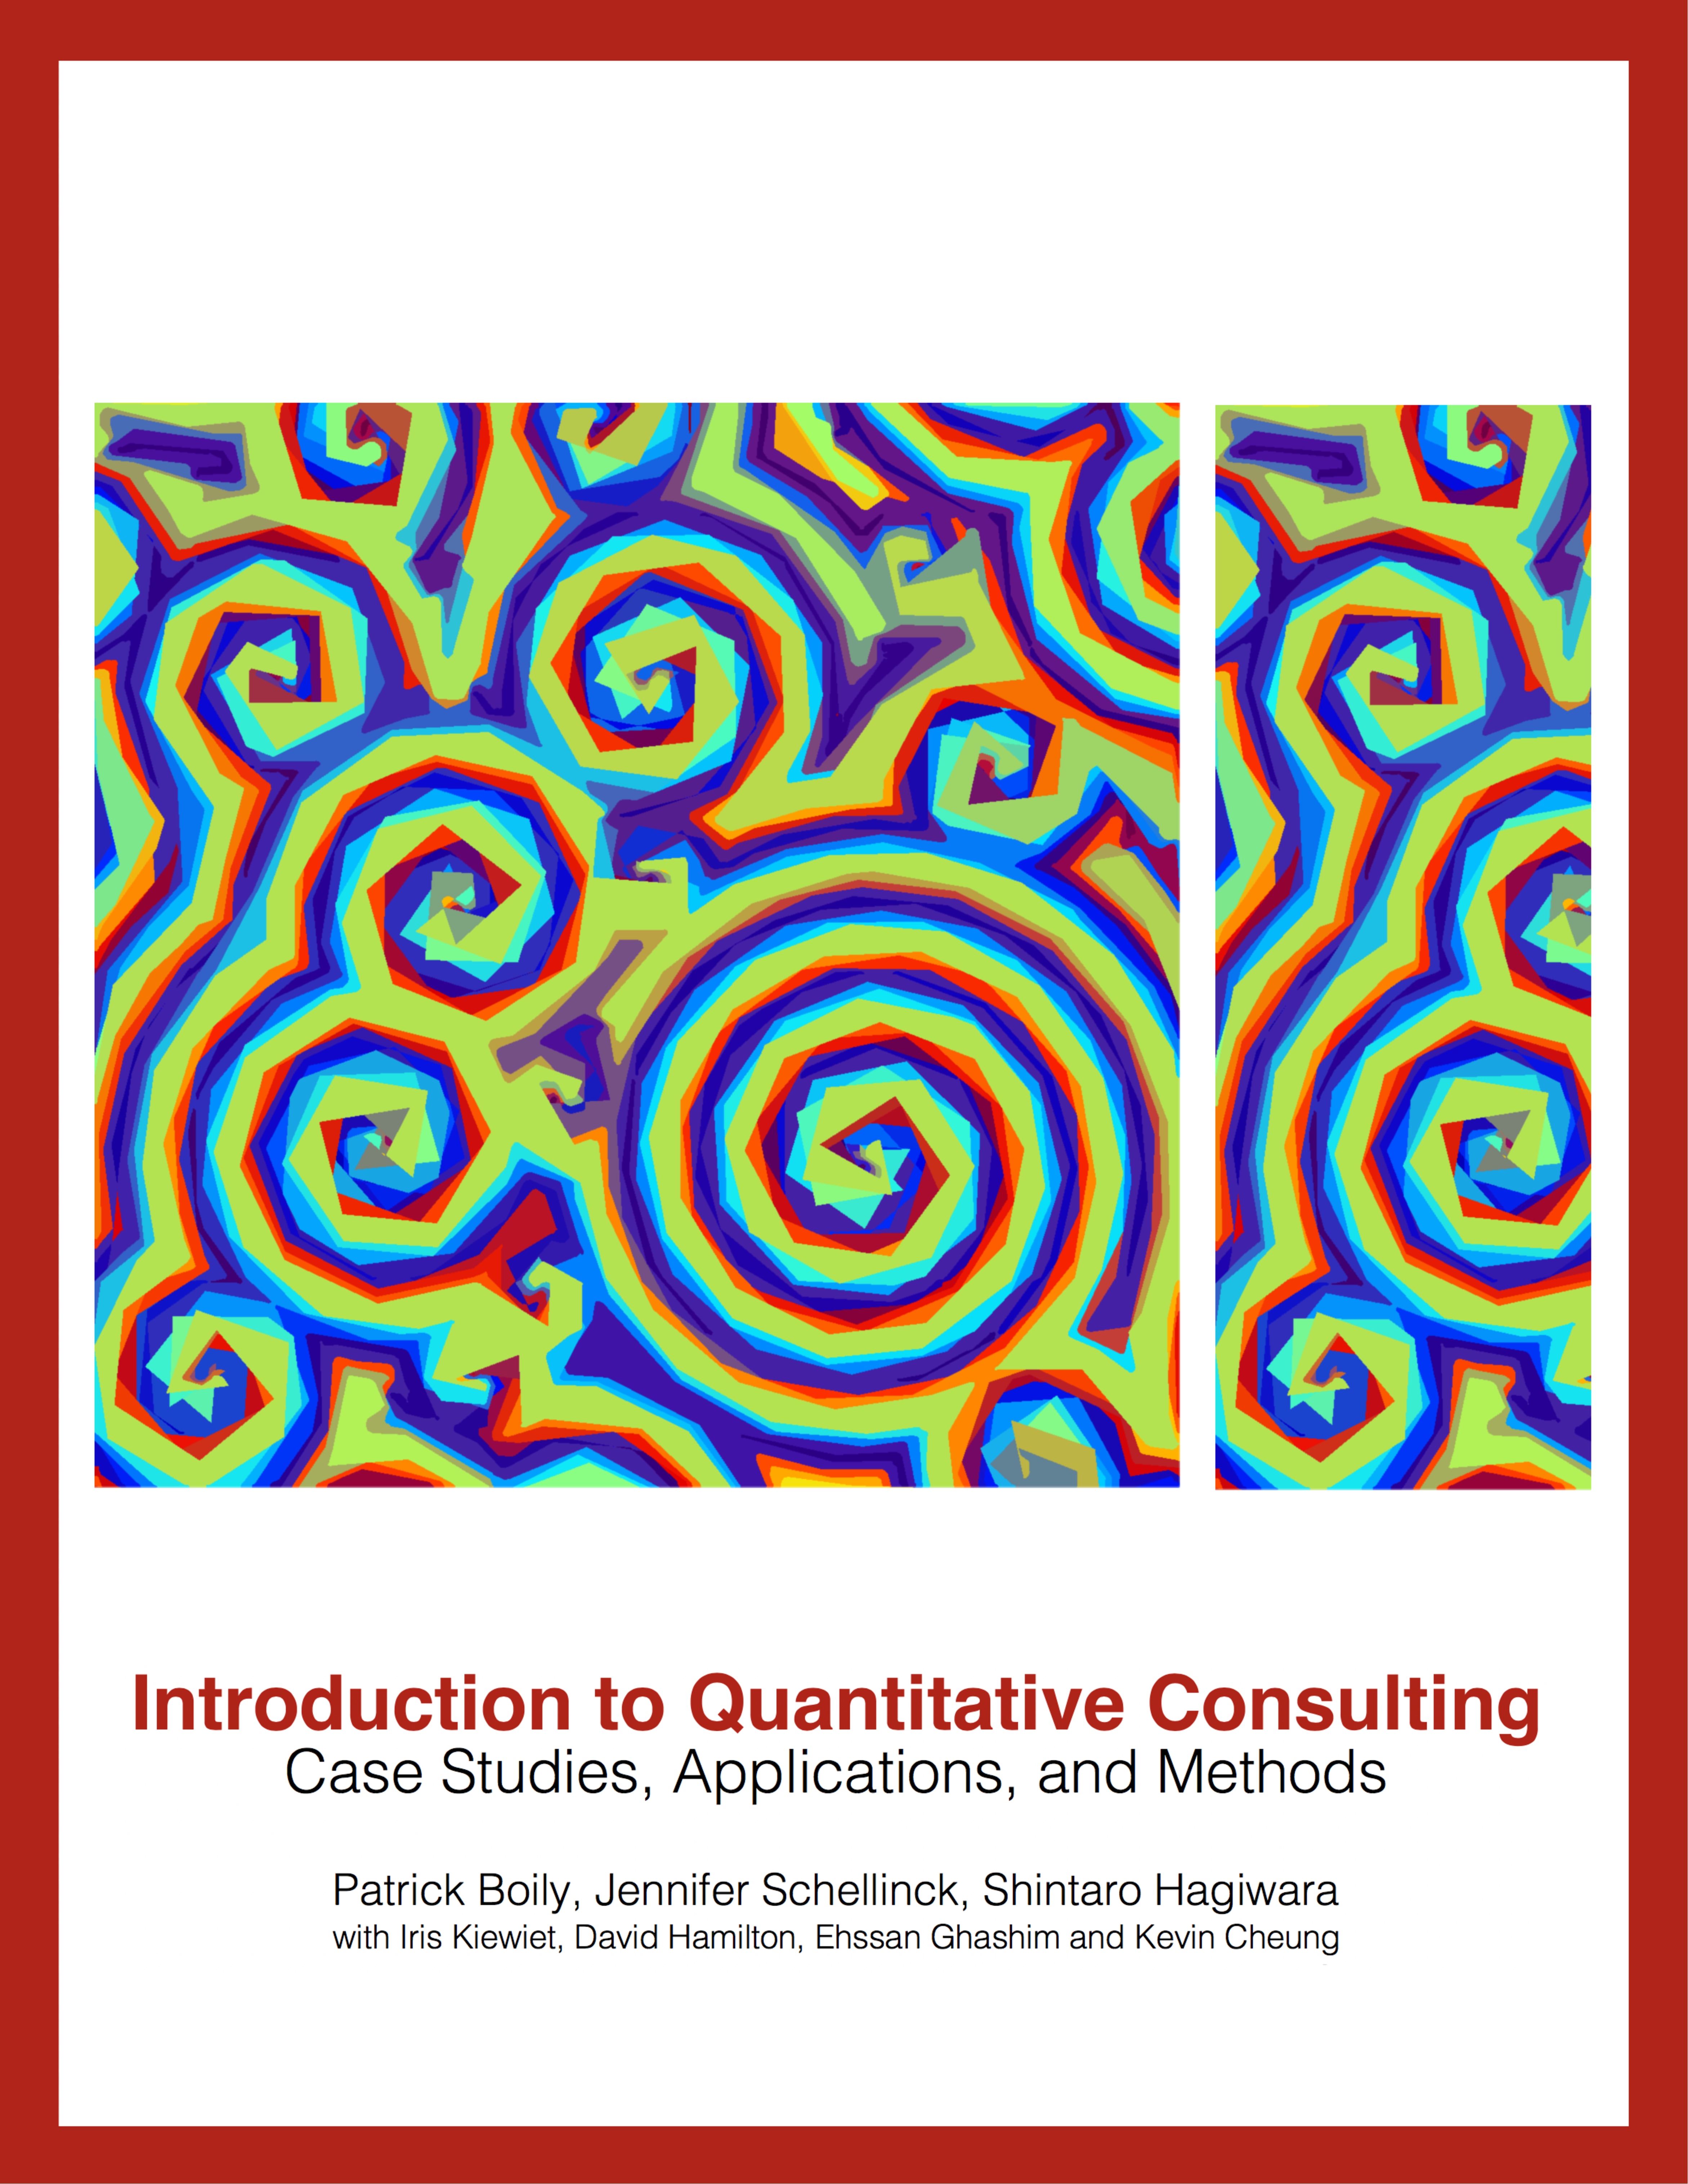
\includegraphics[width=\paperwidth]{documents/Cover.pdf}};
% Author name
%\end{tikzpicture}
%\vfill
%\endgroup
%\thispagestyle{empty}
%\ \newl\newl\newl\newl\newl\begin{center}\Huge{DRAFT}\end{center}



%\headheight = 0pt
%\headsep = 0pt
%\voffset=-1in
%\hoffset=-1in
%\oddsidemargin=0in
%\evensidemargin=0in
%\topmargin=0in
%\textheight=11in
%\textwidth=8.5in

%\begin{center}
%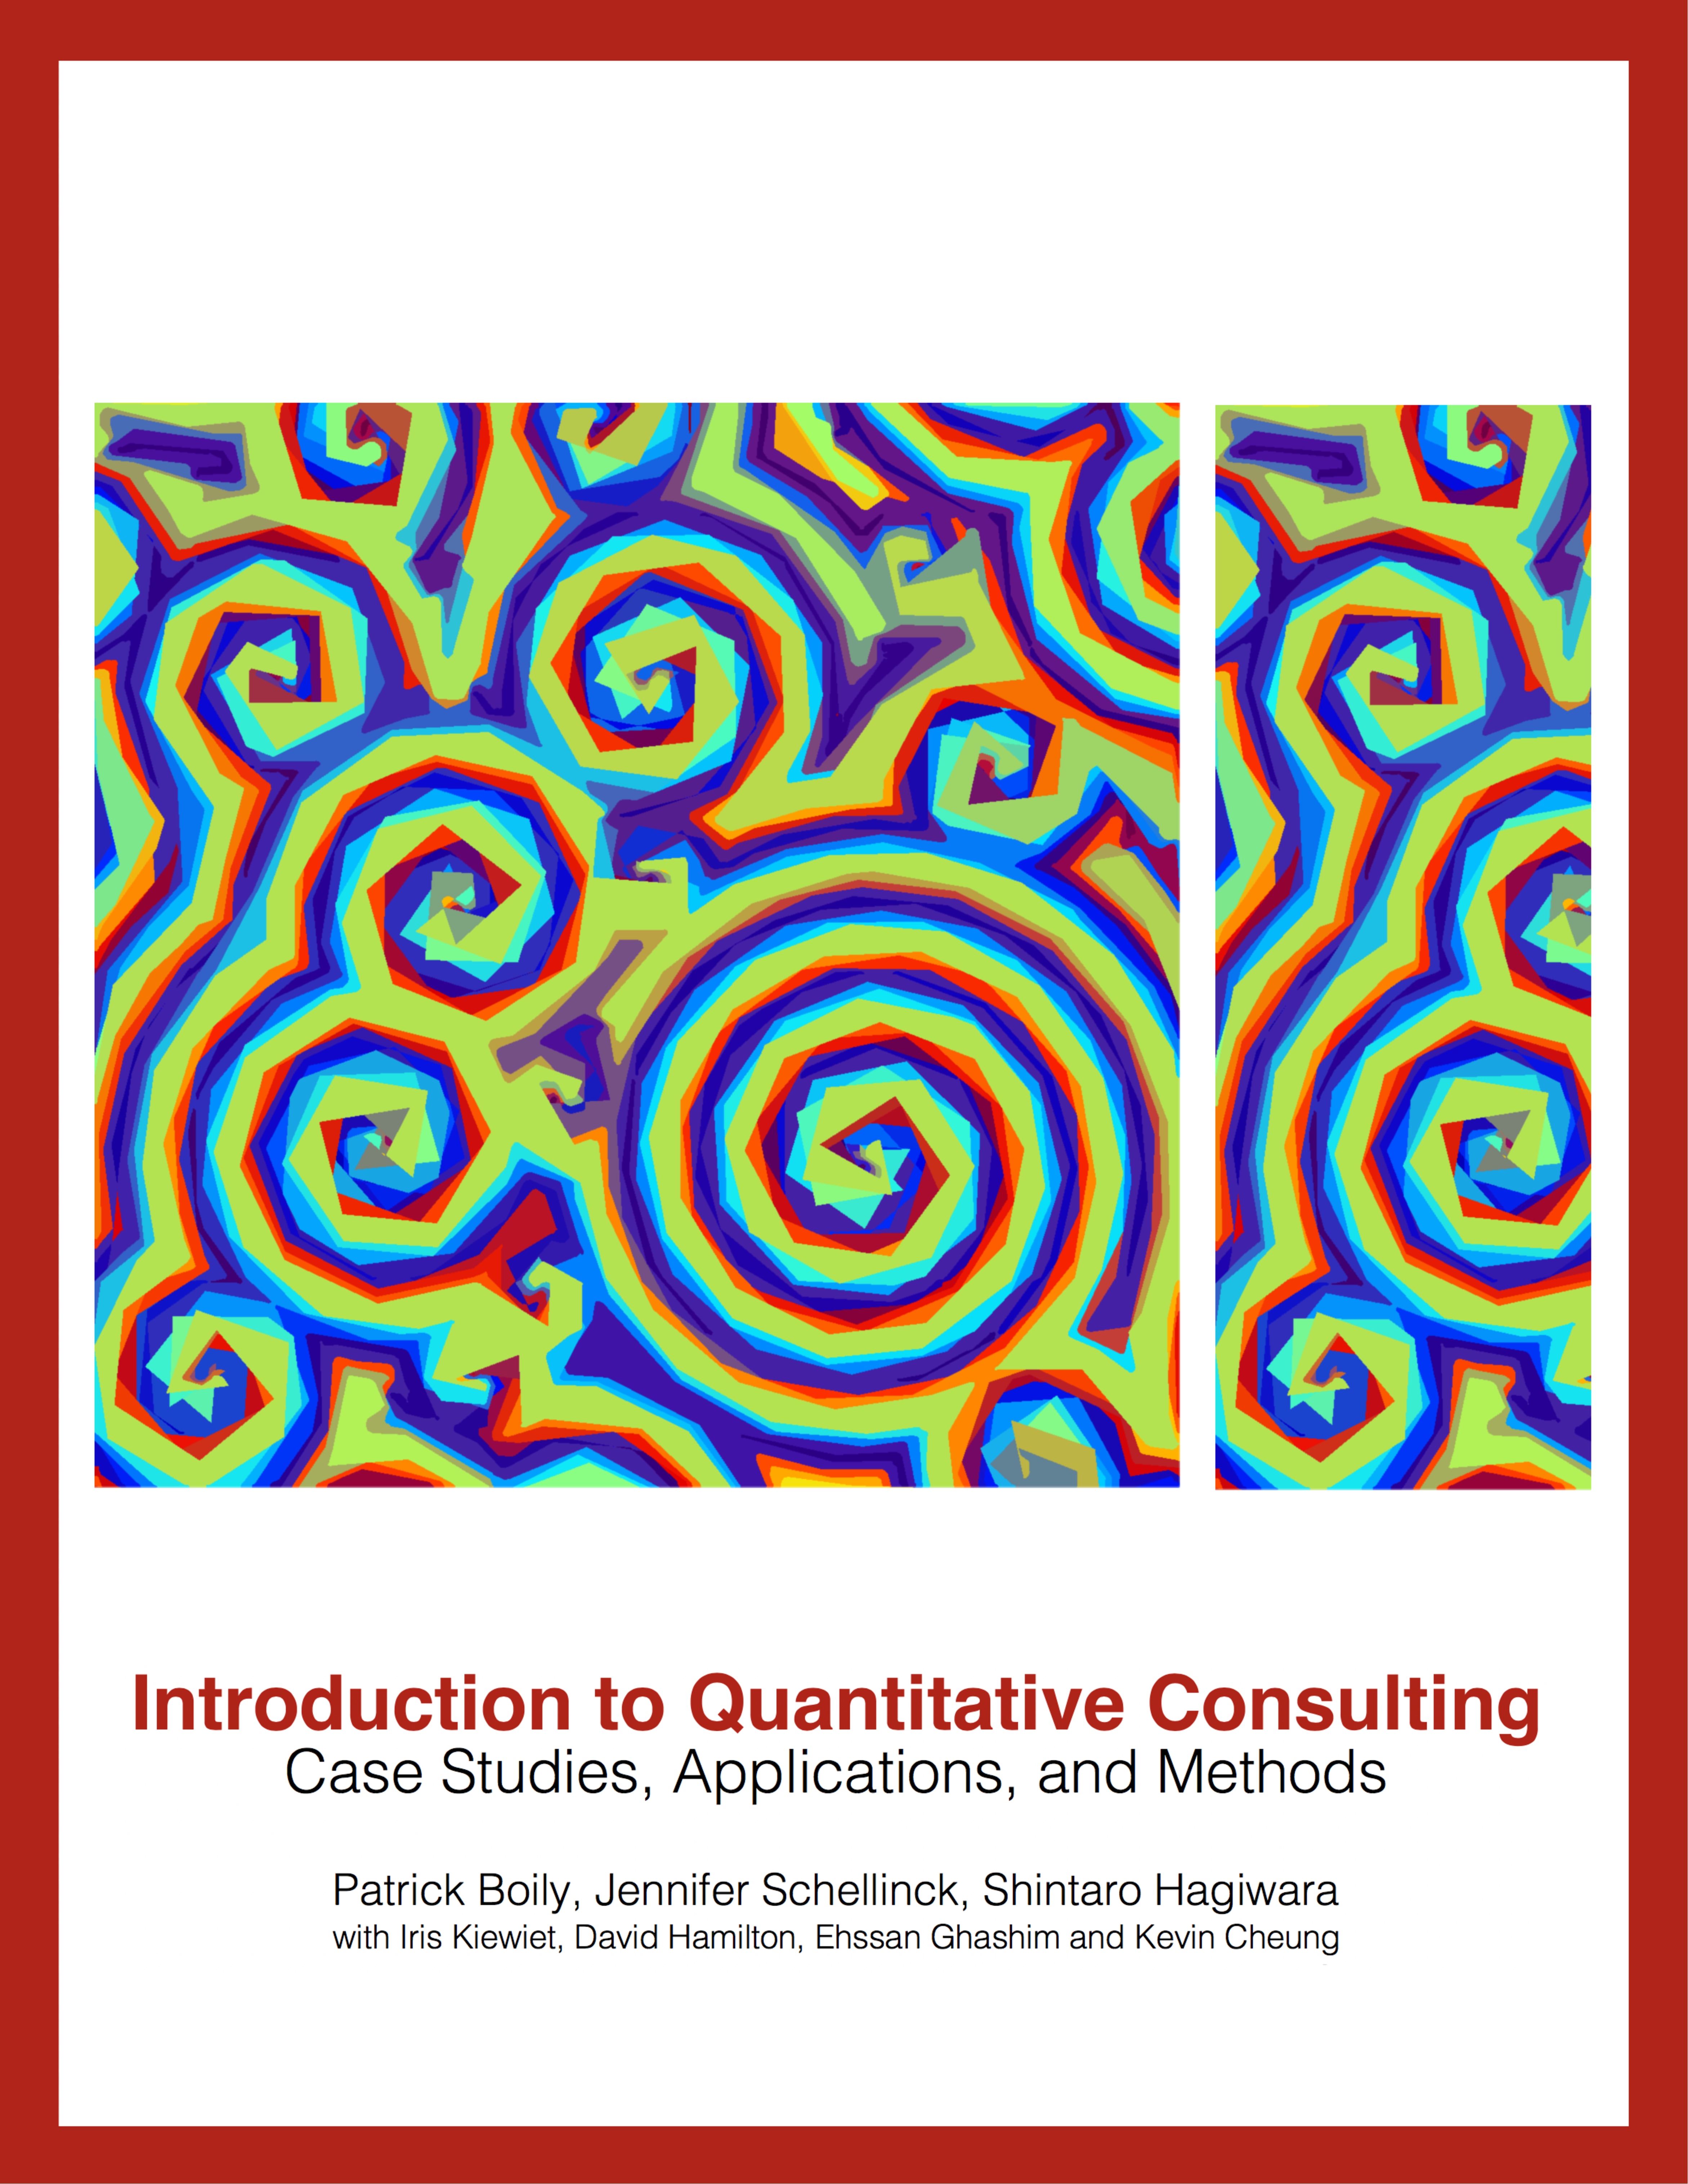
\includegraphics[width=\textwidth]{documents/Cover.pdf}
%\end{center}
%\newpage
%\thispagestyle{empty}
%\noindent Licensed under the Creative Commons/Attribution/Non-Commercial/Share Alike Unported License (the ``License''). You may not use this file except in compliance with the License. You may obtain a copy of the License at \url{http://creativecommons.org/licenses/by-nc-sa/4.0}. Unless required by applicable law or agreed to in writing, software distributed under the License is distributed on an \textsc{``as is'' basis, without warranties or conditions of any kind}, either express or implied. See the License for the specific language governing permissions and limitations under the License.\\ % License information

%\noindent \hfill 
\includegraphics[height=30pt]{images/ZZ/cc.png} 
\includegraphics[height=30pt]{images/ZZ/by.png}  
\includegraphics[height=30pt]{images/ZZ/nc.png} 
\includegraphics[height=30pt]{images/ZZ/sa.png} \\ % Copyright notice

%\noindent \textit{First printing, September 2018} % Printing/edition date
\headheight = 35pt
\headsep = 25pt
\voffset=-.5in
\hoffset=-.75in
\oddsidemargin=0.65in
\evensidemargin=0.65in
\topmargin=-0.15in
\textheight=9.1in
\textwidth=6.7in
\newpage 
%\thispagestyle{empty}
%\section*{Acknowledgments}
%We would like to acknowledge the many individuals and organisations that have made this work possible: Dong Liu, Katrina Rogers-Stewart, Lani Haque, Andrew Macfie, Yue Huang, Yao Ying, Colin Daniel, Yiqiang Zhao, Malcolm Butler, Korey MacDougall, and Pat Farrell. 
%\newpage


\tableofcontents 
\listoffigures
\listoftables

\pagestyle{fancy}
\lhead[\textsc{\newtitle}]{P Boily, J Schellinck, S Hagiwara \thedraft}
\rhead[P Boily, J Schellinck, S Hagiwara \thedraft]{\textsc{\rightmark}}
\chead{}
\rfoot[\footnotesize\thepage]{\footnotesize{\thedraft}}
\cfoot{}
\lfoot[\footnotesize{\thedraft}]{\footnotesize{\thepage}}

\newpage\noindent
%\section{Consulting Landscape}
   \addtocounter{subsection}{1}
\addcontentsline{toc}{subsection}{\protect\numberline{\thesubsection}Introduction}
\setboolean{@twoside}{false}
\includepdf[pages={1-3},offset={50 -40}]{documents/Consulting_Intro_book.pdf}
   \addtocounter{subsubsection}{1}
\addcontentsline{toc}{subsubsection}{\protect\numberline{\thesubsubsection}The Consulting Framework}
\includepdf[pages={4-6},offset={50 -40}]{documents/Consulting_Intro_book.pdf}
   \addtocounter{subsubsection}{1}
\addcontentsline{toc}{subsubsection}{\protect\numberline{\thesubsubsection}Ethical Considerations}
\includepdf[pages={7-11},offset={50 -40}]{documents/Consulting_Intro_book.pdf}
   \addtocounter{subsubsection}{1}
\addcontentsline{toc}{subsubsection}{\protect\numberline{\thesubsubsection}Guiding Principles}
\includepdf[pages={12-15},offset={50 -40}]{documents/Consulting_Intro_book.pdf}
   \addtocounter{subsubsection}{1}
\addcontentsline{toc}{subsubsection}{\protect\numberline{\thesubsubsection}Asking the Right Questions}
\includepdf[pages={16-17},offset={50 -40}]{documents/Consulting_Intro_book.pdf}
   \addtocounter{subsubsection}{1}
\addcontentsline{toc}{subsubsection}{\protect\numberline{\thesubsubsection}The Structure of Data}
\includepdf[pages={18-22},offset={50 -40}]{documents/Consulting_Intro_book.pdf}
   \addtocounter{subsubsection}{1}
\addcontentsline{toc}{subsubsection}{\protect\numberline{\thesubsubsection}Quantitative Consulting Workflows}
\includepdf[pages={23-30},offset={50 -40}]{documents/Consulting_Intro_book.pdf}
   \addtocounter{subsubsection}{1}
\addcontentsline{toc}{subsubsection}{\protect\numberline{\thesubsubsection}Roles and Responsibilities}
\includepdf[pages={31-36},offset={50 -40}]{documents/Consulting_Intro_book.pdf}
   \addtocounter{subsubsection}{1}
\addcontentsline{toc}{subsubsection}{\protect\numberline{\thesubsubsection}Consulting Cheat Sheet}
\includepdf[pages={37-39},offset={50 -40}]{documents/Consulting_Intro_book.pdf}
   \addtocounter{subsection}{1}
\addcontentsline{toc}{subsection}{\protect\numberline{\thesubsection}Consulting Lifecycle}
   \includepdf[pages={1},offset={50 -40}]{documents/Consulting_lifecycle_book.pdf}
\setcounter{subsubsection}{0}
\addtocounter{subsubsection}{1}
\addcontentsline{toc}{subsubsection}{\protect\numberline{\thesubsubsection}Consulting Lifecycle}
   \includepdf[pages={2-25},offset={50 -40}]{documents/Consulting_lifecycle_book.pdf}
   \addtocounter{subsubsection}{1}
\addcontentsline{toc}{subsubsection}{\protect\numberline{\thesubsubsection}Lessons Learned}
   \includepdf[pages={26-31},offset={50 -40}]{documents/Consulting_lifecycle_book.pdf}
   \addtocounter{subsection}{1}
\addcontentsline{toc}{subsection}{\protect\numberline{\thesubsection}Practical Interactions with Clients}
\setcounter{subsubsection}{0}
   \addtocounter{subsubsection}{1}
\addcontentsline{toc}{subsubsection}{\protect\numberline{\thesubsubsection}Business Development}
      \includepdf[pages={1-2},offset={50 -40}]{documents/Consulting_bd_book.pdf}
   \addtocounter{subsubsection}{1}
\addcontentsline{toc}{subsubsection}{\protect\numberline{\thesubsubsection}Cients and Choices}
   \includepdf[pages={3-4},offset={50 -40}]{documents/Consulting_bd_book.pdf}
   \addtocounter{subsubsection}{1}
\addcontentsline{toc}{subsubsection}{\protect\numberline{\thesubsubsection}Building Trust}
   \includepdf[pages={5-9},offset={50 -40}]{documents/Consulting_bd_book.pdf}
   \addtocounter{subsubsection}{1}
\addcontentsline{toc}{subsubsection}{\protect\numberline{\thesubsubsection}Improving Trust}
   \includepdf[pages={10-16},offset={50 -40}]{documents/Consulting_bd_book.pdf}
   \addtocounter{subsection}{1}
\addcontentsline{toc}{subsection}{\protect\numberline{\thesubsection}Technical Writing}
\setcounter{subsubsection}{0}
   \addtocounter{subsubsection}{1}
\addcontentsline{toc}{subsubsection}{\protect\numberline{\thesubsubsection}What is Technical Writing}
   \includepdf[pages={1-4},offset={50 -40}]{documents/Consulting_TW_book.pdf}
   \addtocounter{subsubsection}{1}
\addcontentsline{toc}{subsubsection}{\protect\numberline{\thesubsubsection}The Five Components of Technical Writing}
   \includepdf[pages={5-17},offset={50 -40}]{documents/Consulting_TW_book.pdf}
   \addtocounter{subsubsection}{1}
\addcontentsline{toc}{subsubsection}{\protect\numberline{\thesubsubsection}Traits of Technical Writing}
   \includepdf[pages={18-30},offset={50 -40}]{documents/Consulting_TW_book.pdf}
\addtocounter{subsection}{1}
\addcontentsline{toc}{subsection}{\protect\numberline{\thesubsection}Samples}
\setcounter{subsubsection}{0}
\addtocounter{subsubsection}{1}
\addcontentsline{toc}{subsubsection}{\protect\numberline{\thesubsubsection}Contracts}
 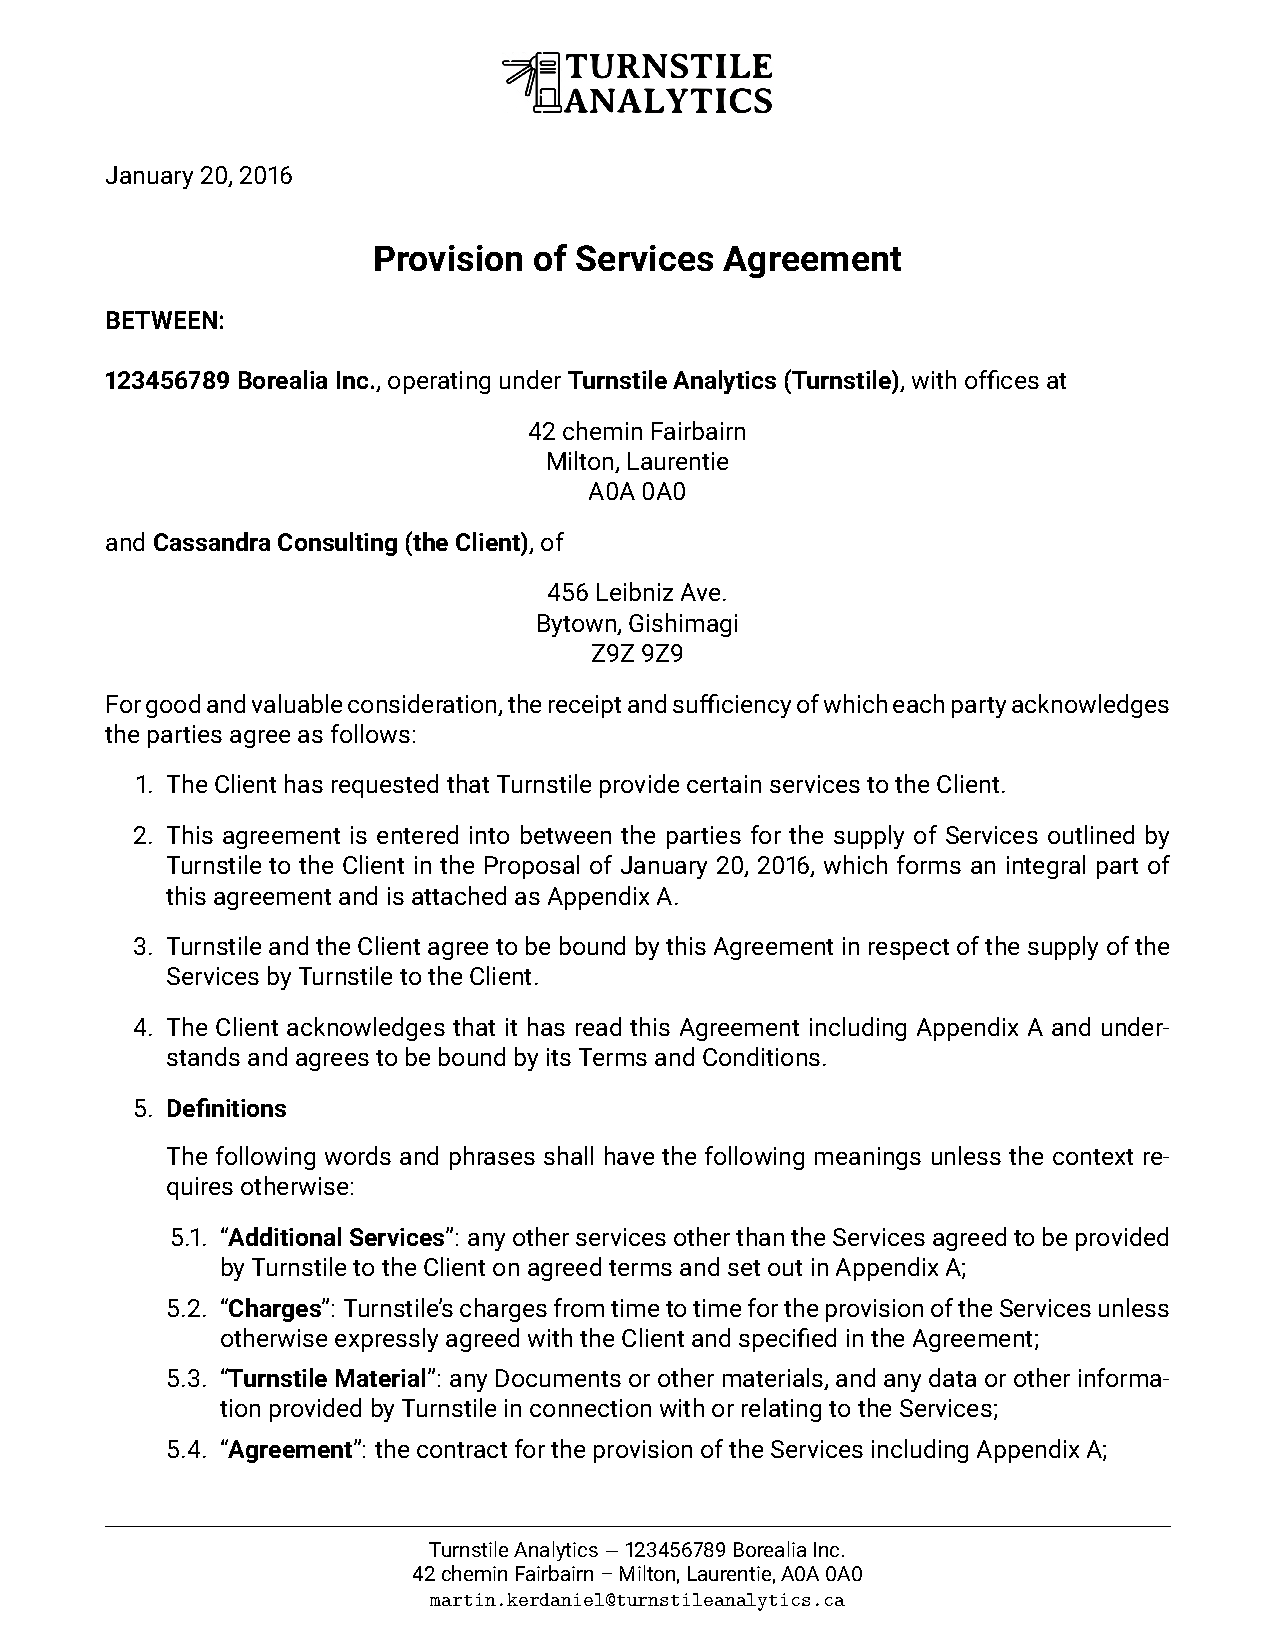
\includepdf[pages={1-7},offset={50 -40}]{documents/PSAE.pdf}
\addtocounter{subsubsection}{1}
\addcontentsline{toc}{subsubsection}{\protect\numberline{\thesubsubsection}Curriculum Vitae}
 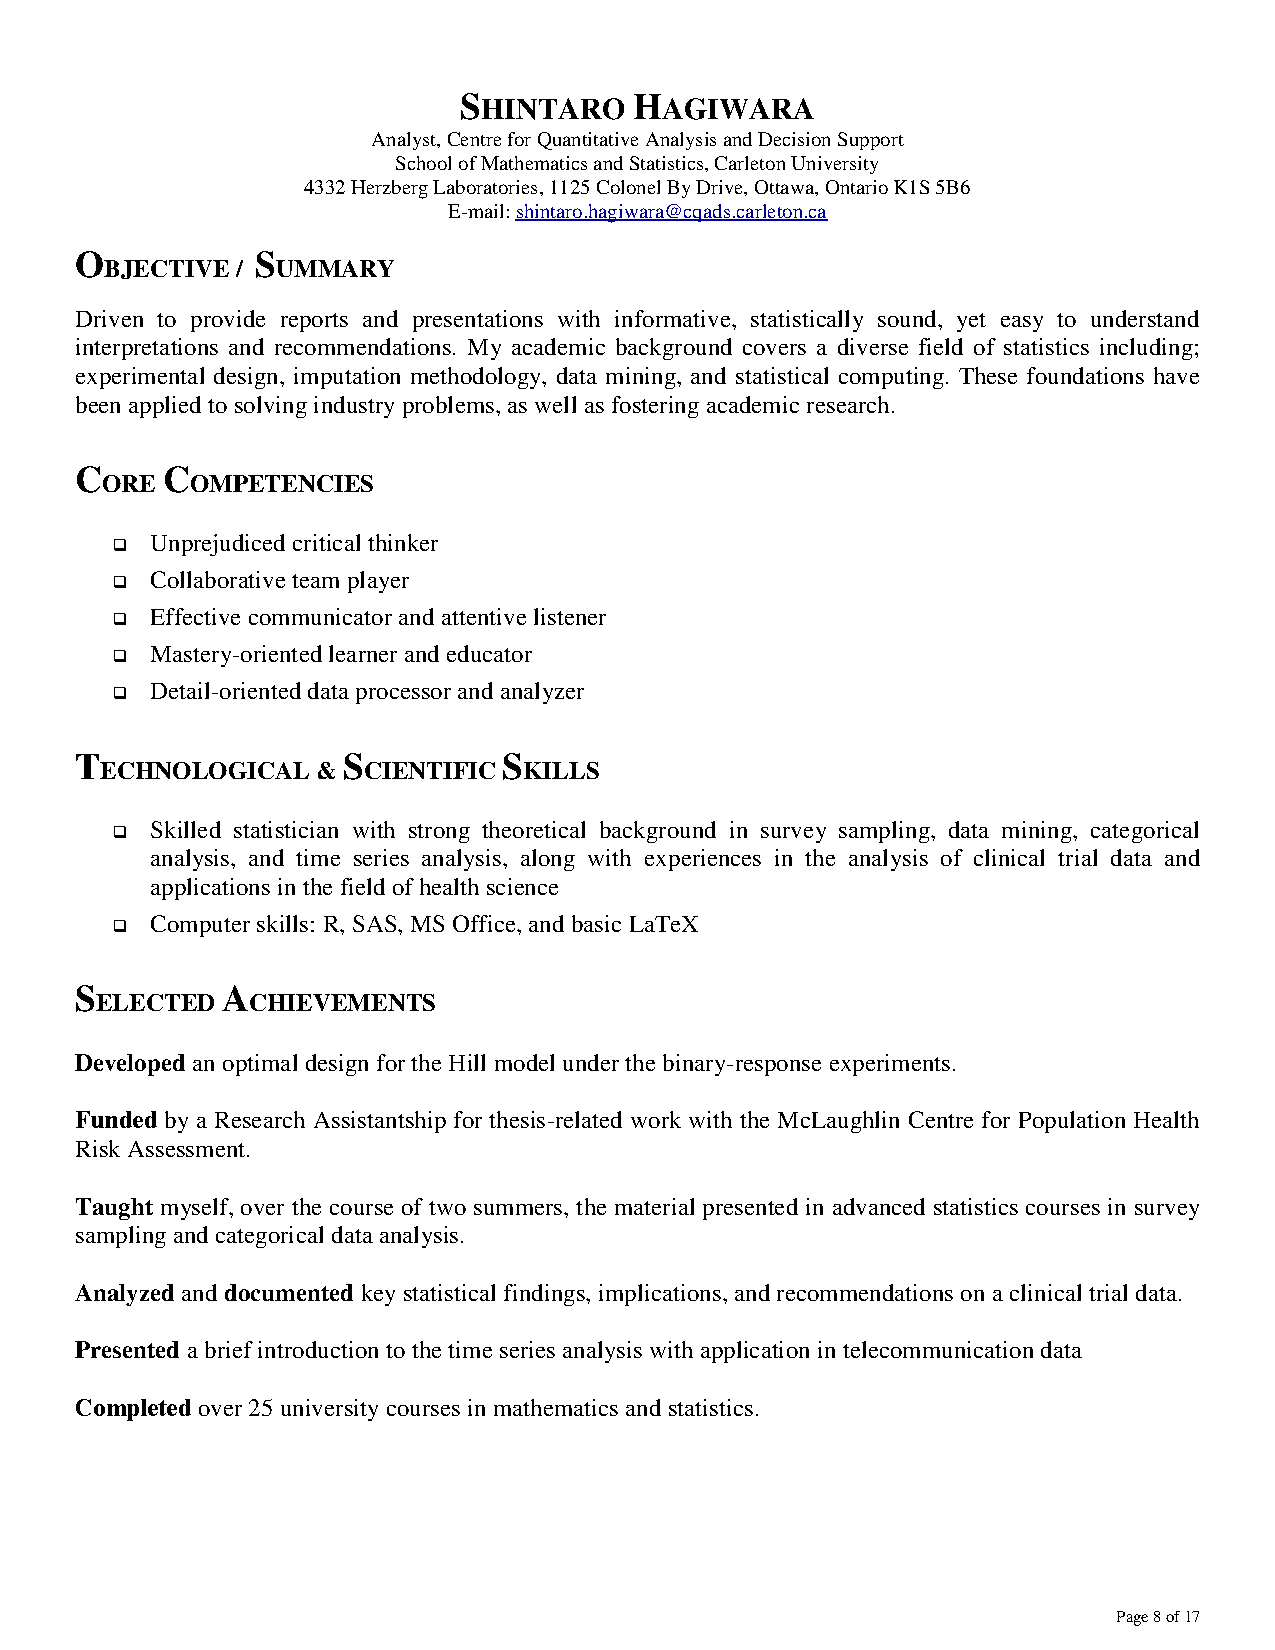
\includepdf[pages={1-2},offset={50 -40}]{documents/SHCV1.pdf}
 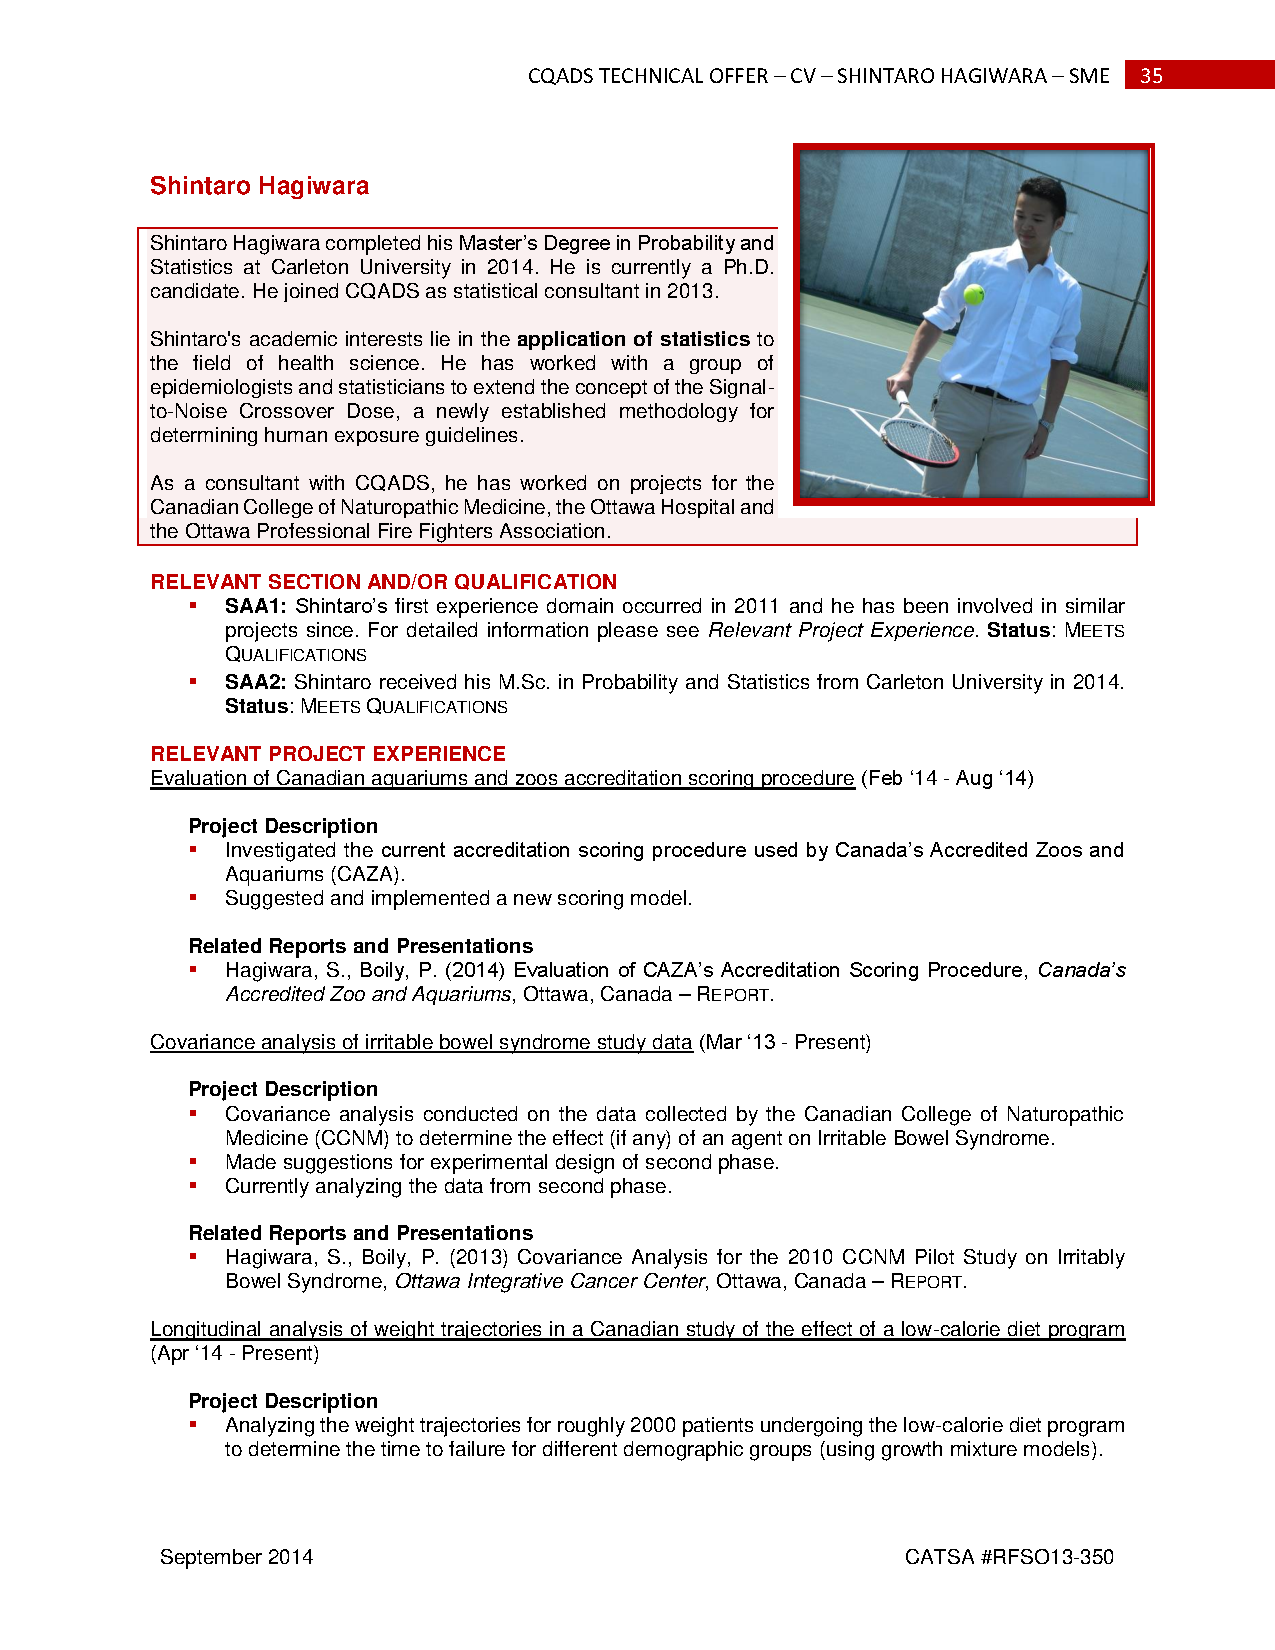
\includepdf[pages={1-2},offset={50 -40}]{documents/SHCV2.pdf}
 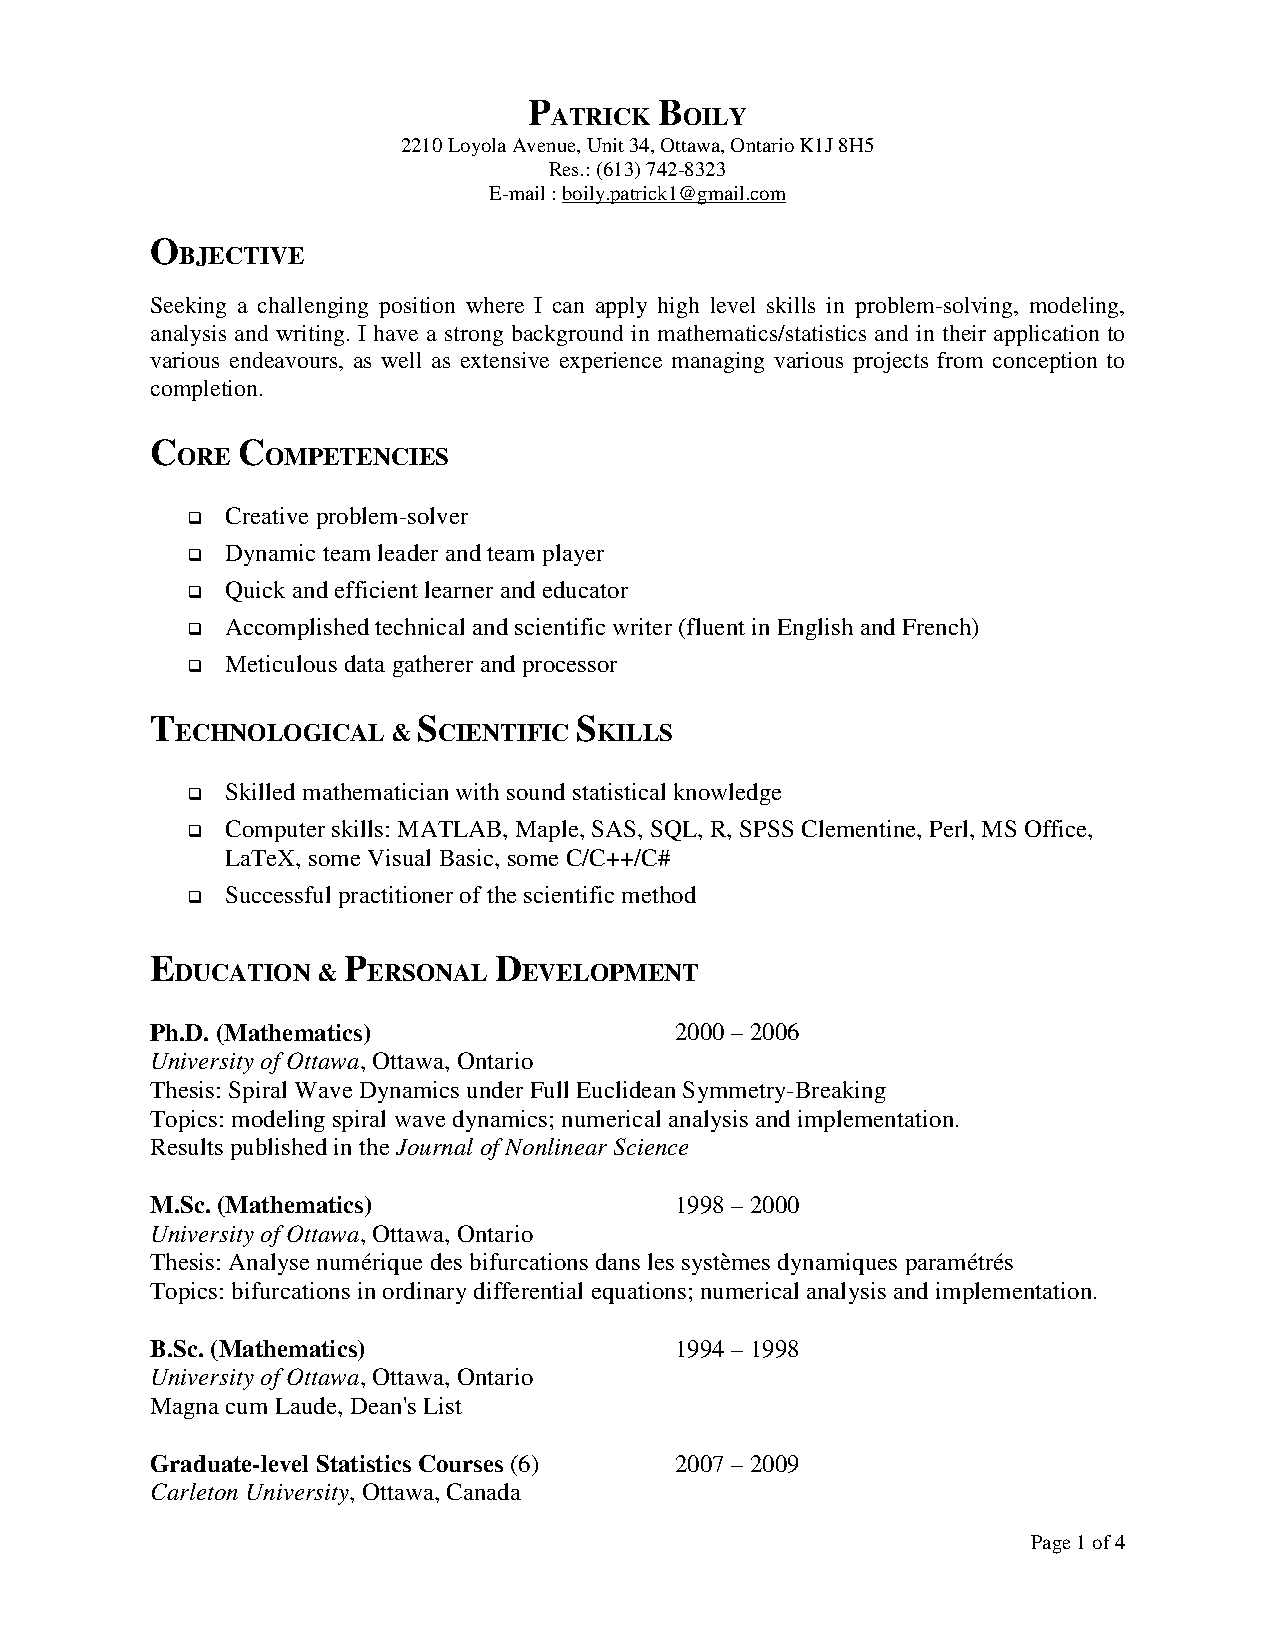
\includepdf[pages={1-4},offset={50 -40}]{documents/PBCV1.pdf}
 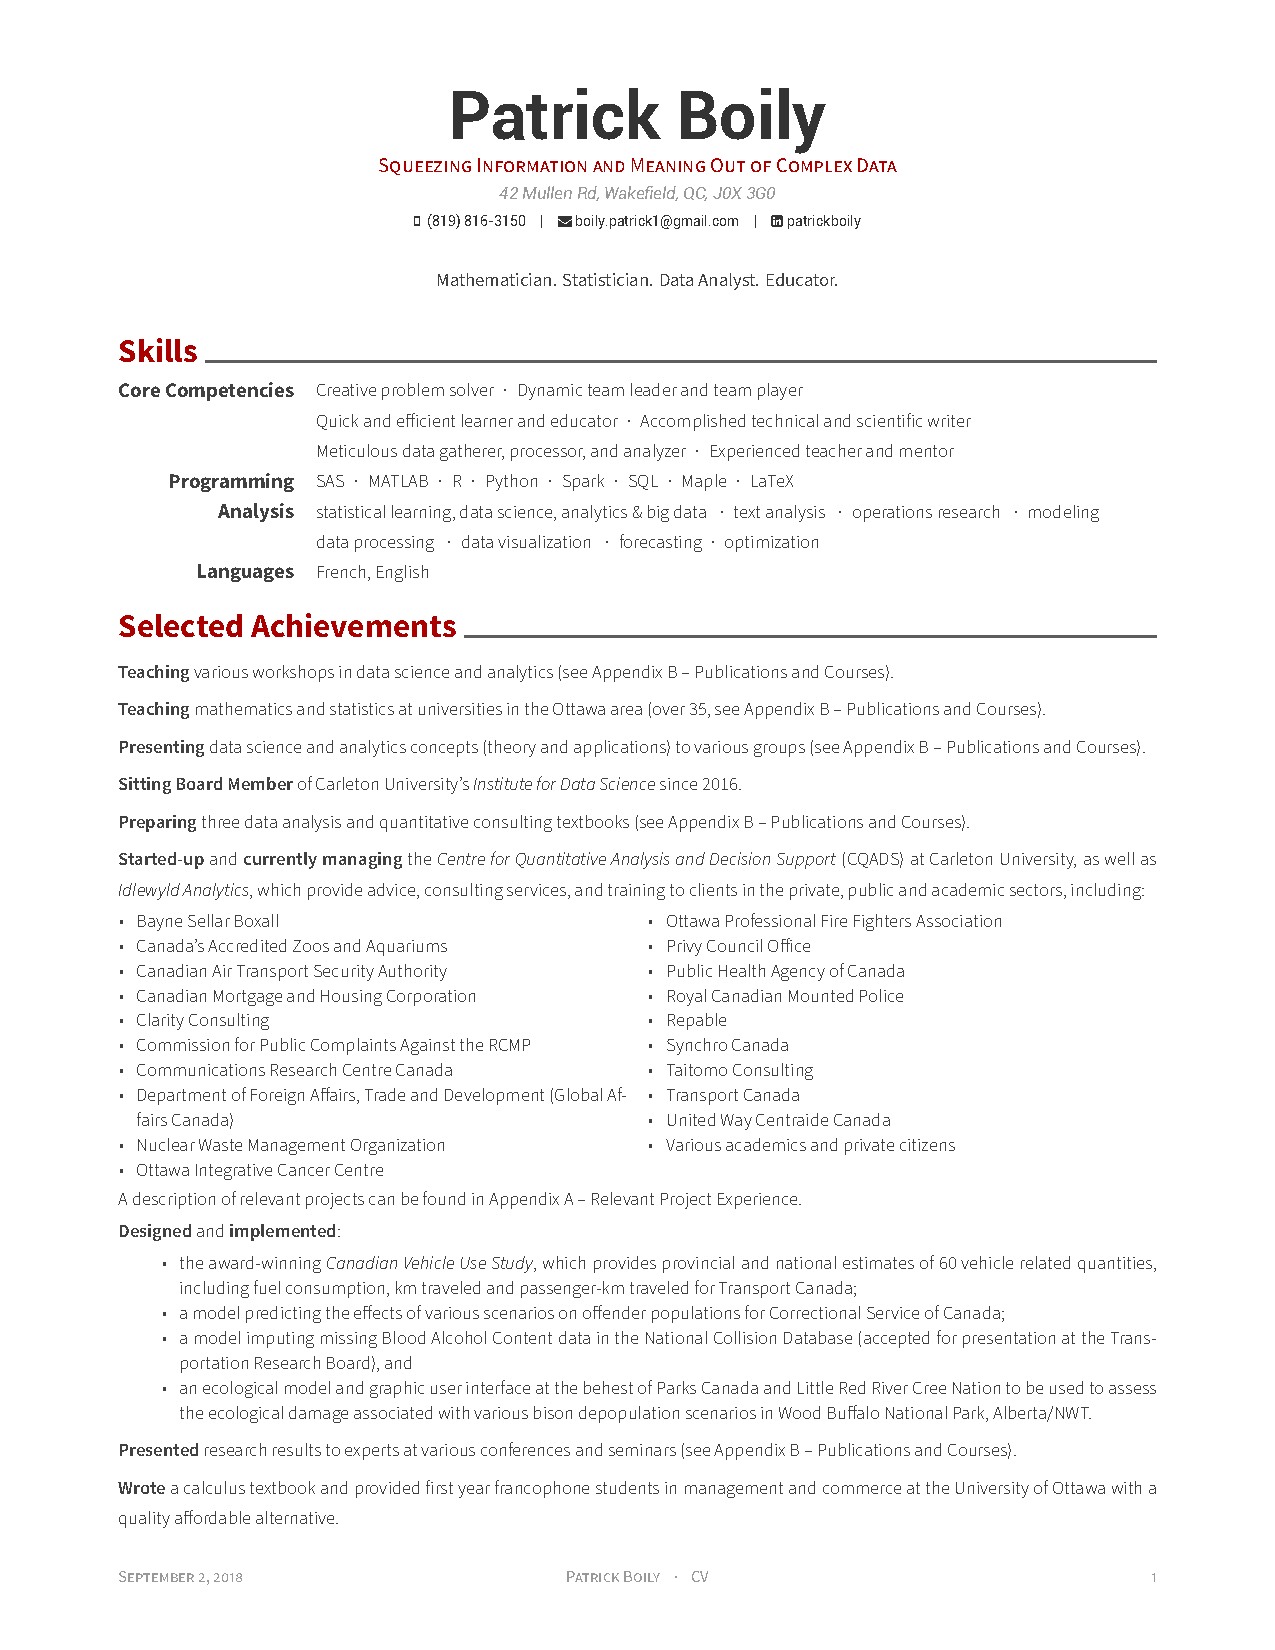
\includepdf[pages={1-14},offset={50 -40}]{documents/PBCV2.pdf}
 \includepdf[pages={11-16},offset={50 -40}]{documents/Pr_GAC1.pdf}
 \addtocounter{subsubsection}{1}
\addcontentsline{toc}{subsubsection}{\protect\numberline{\thesubsubsection}Websites}
 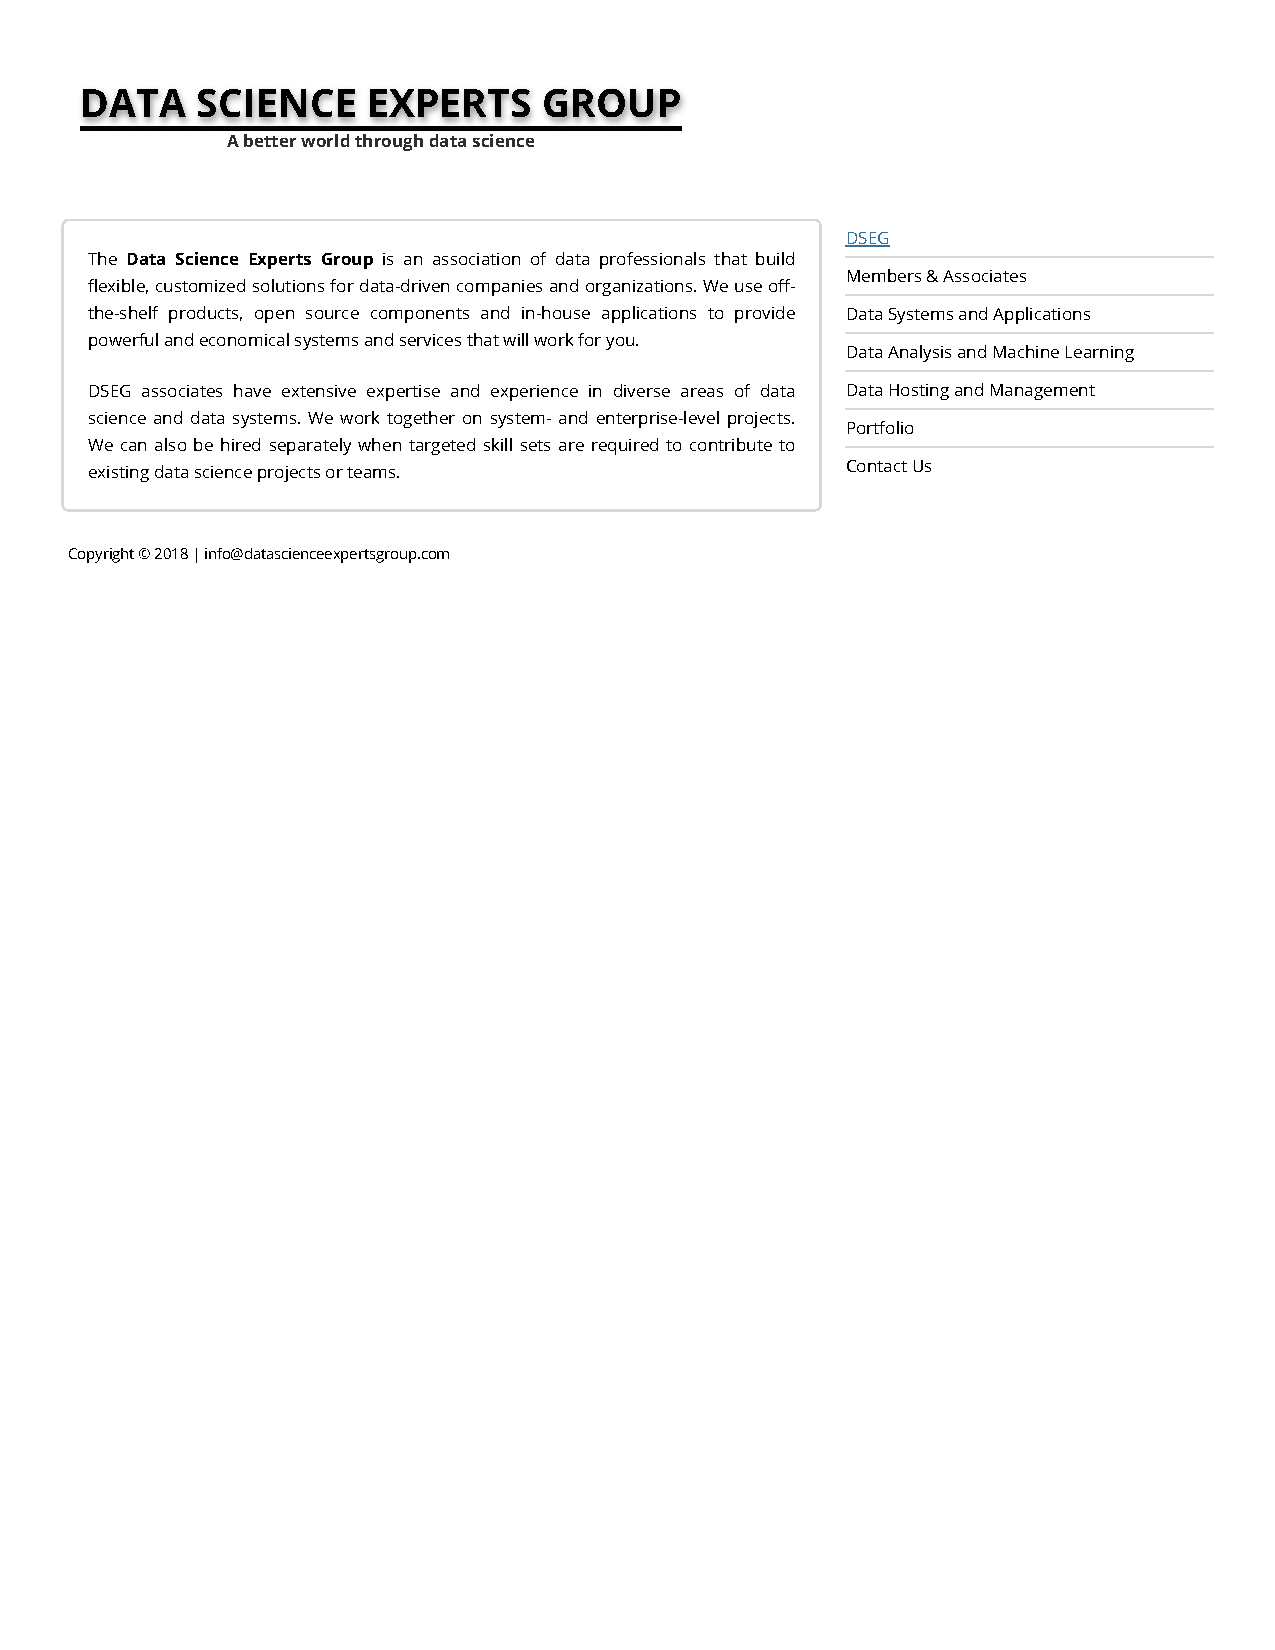
\includepdf[pages={1},offset={50 -40}]{documents/DSEG1.pdf}
 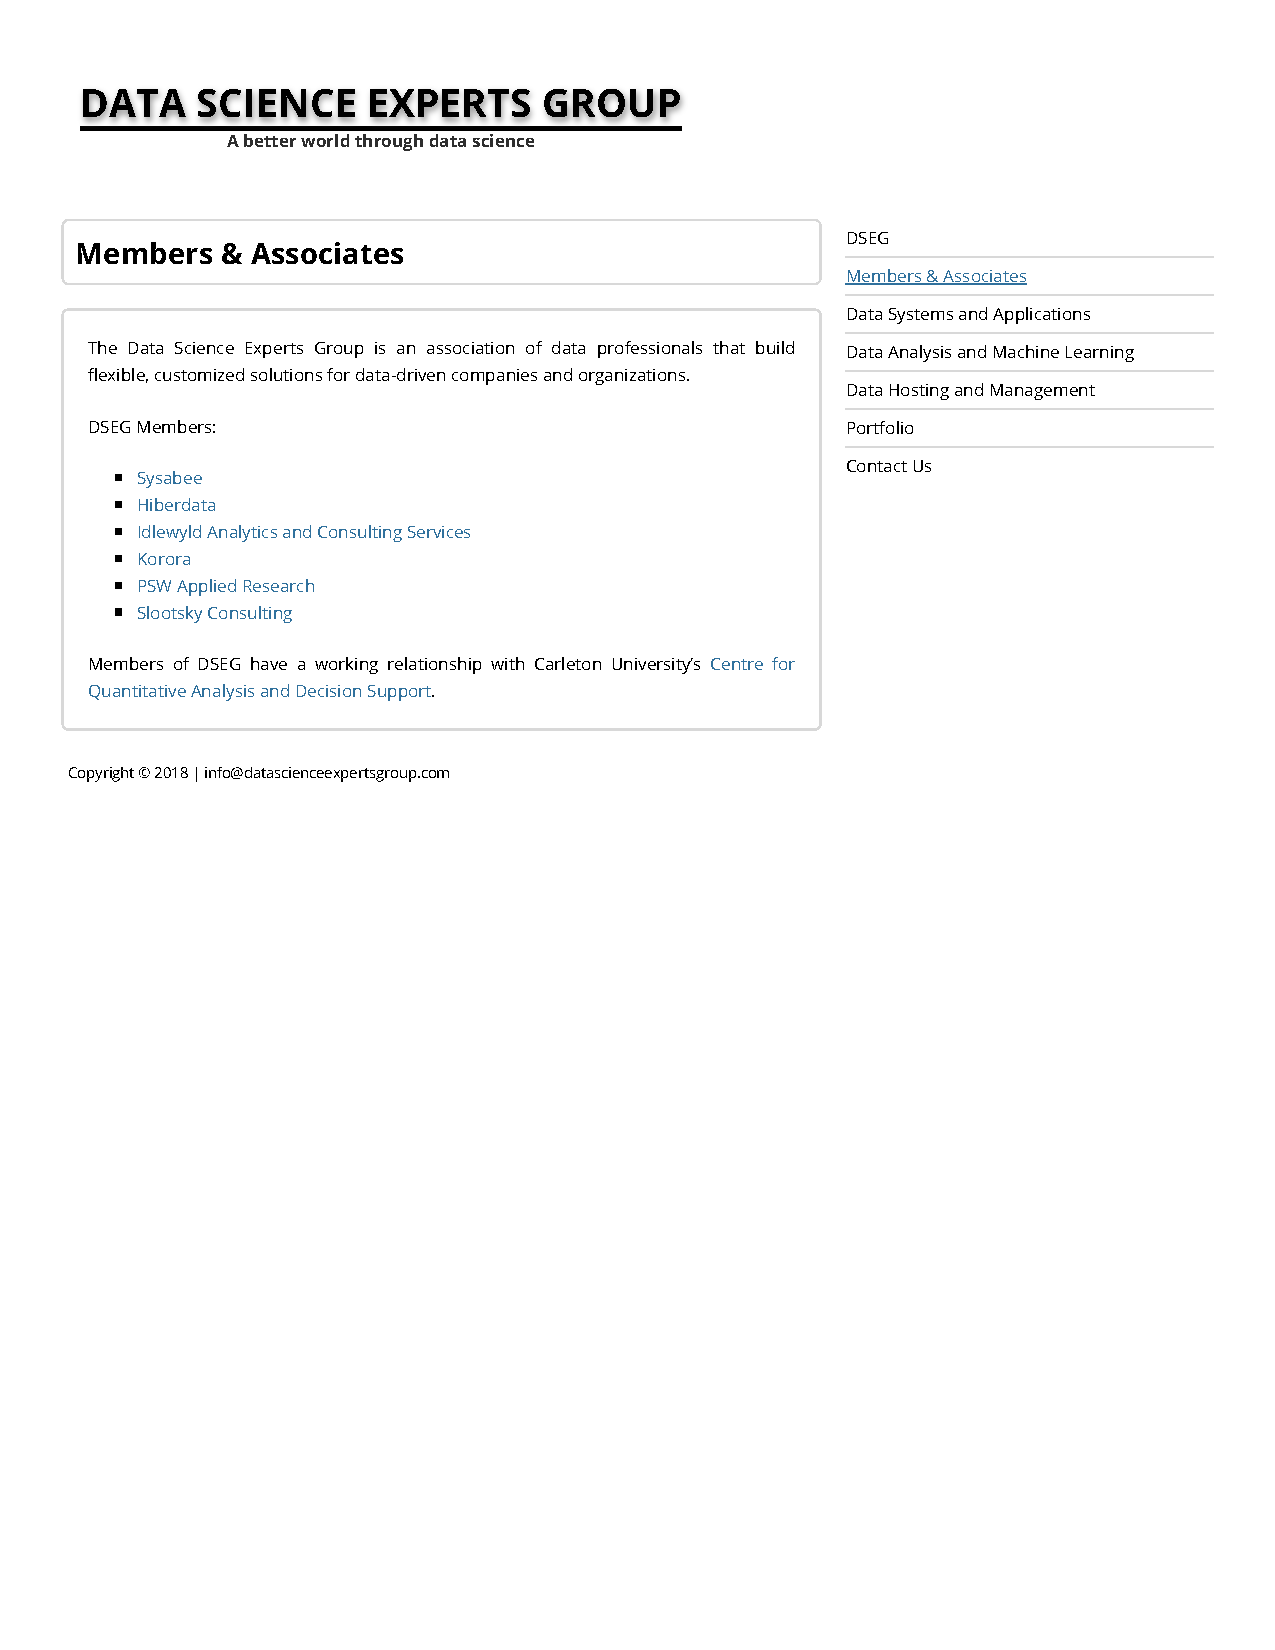
\includepdf[pages={1},offset={50 -40}]{documents/DSEG2.pdf}
 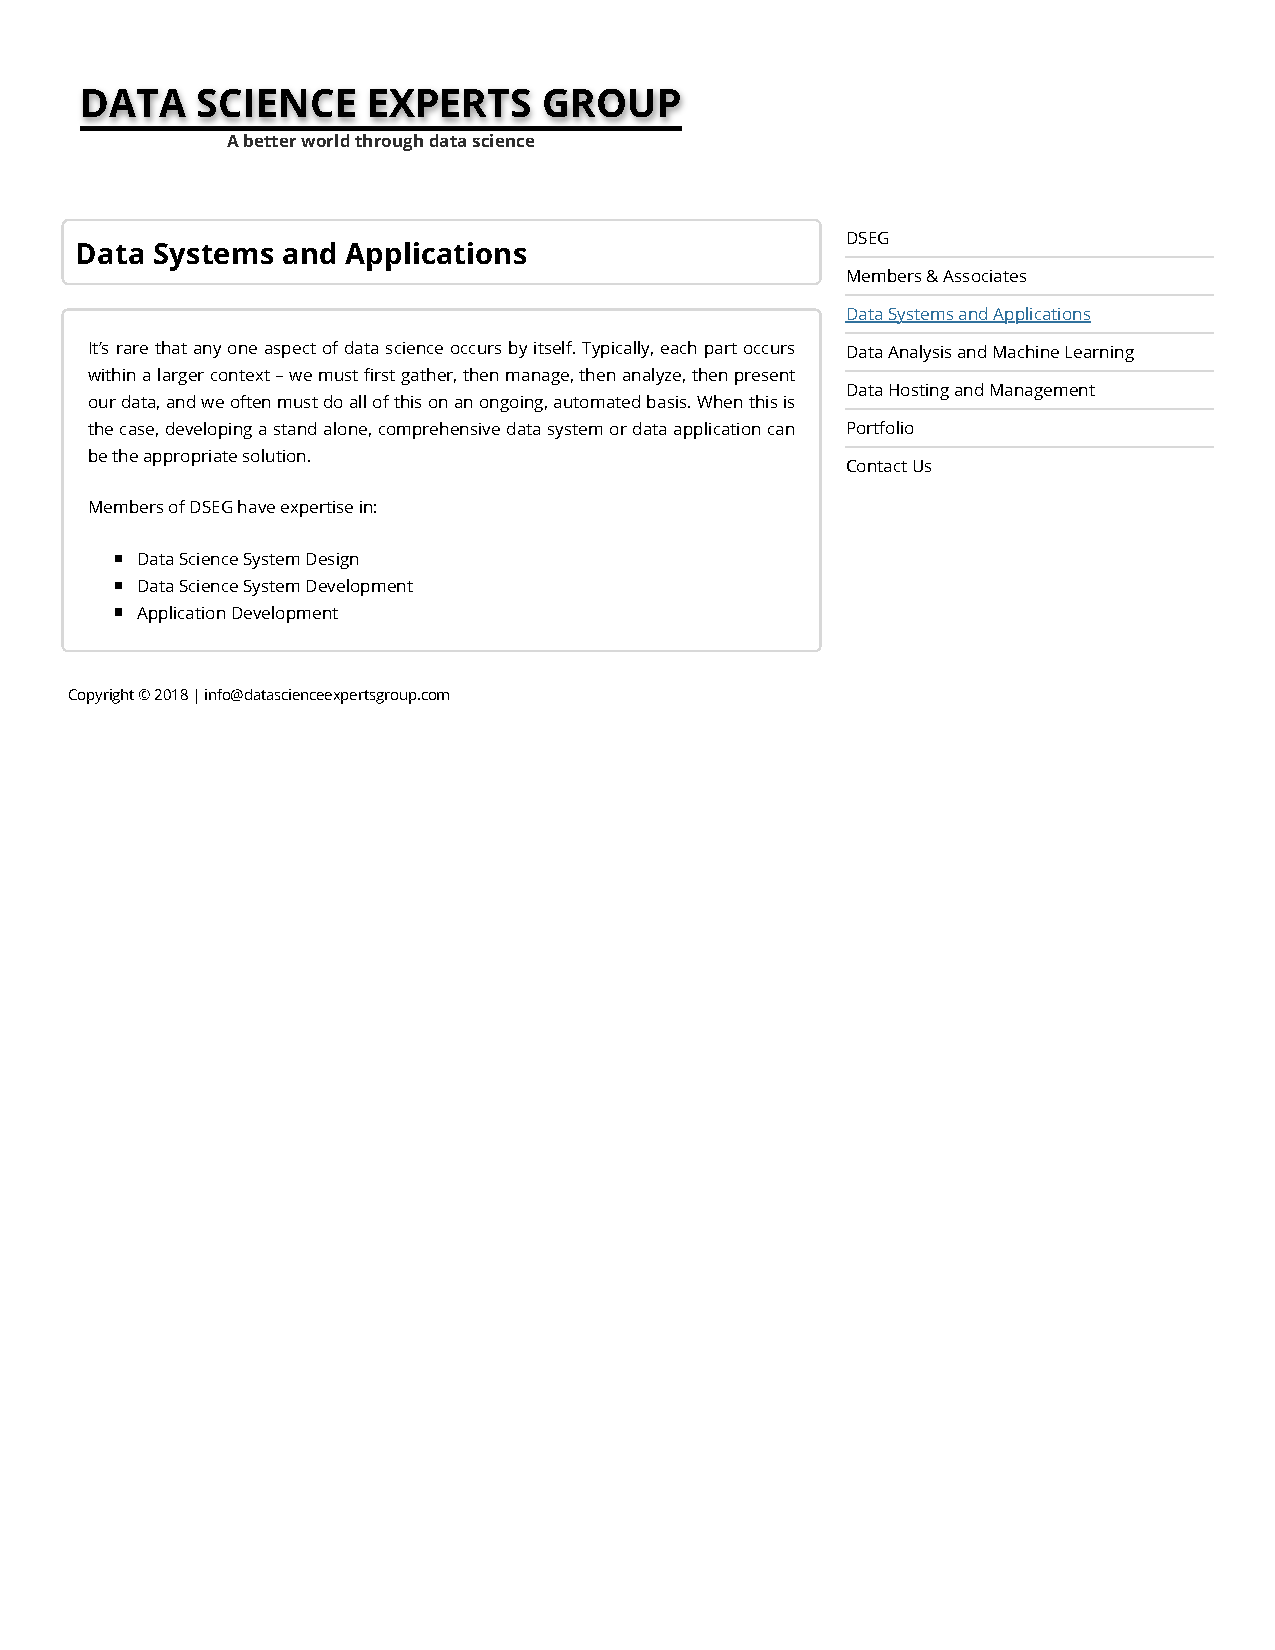
\includepdf[pages={1},offset={50 -40}]{documents/DSEG3.pdf}
 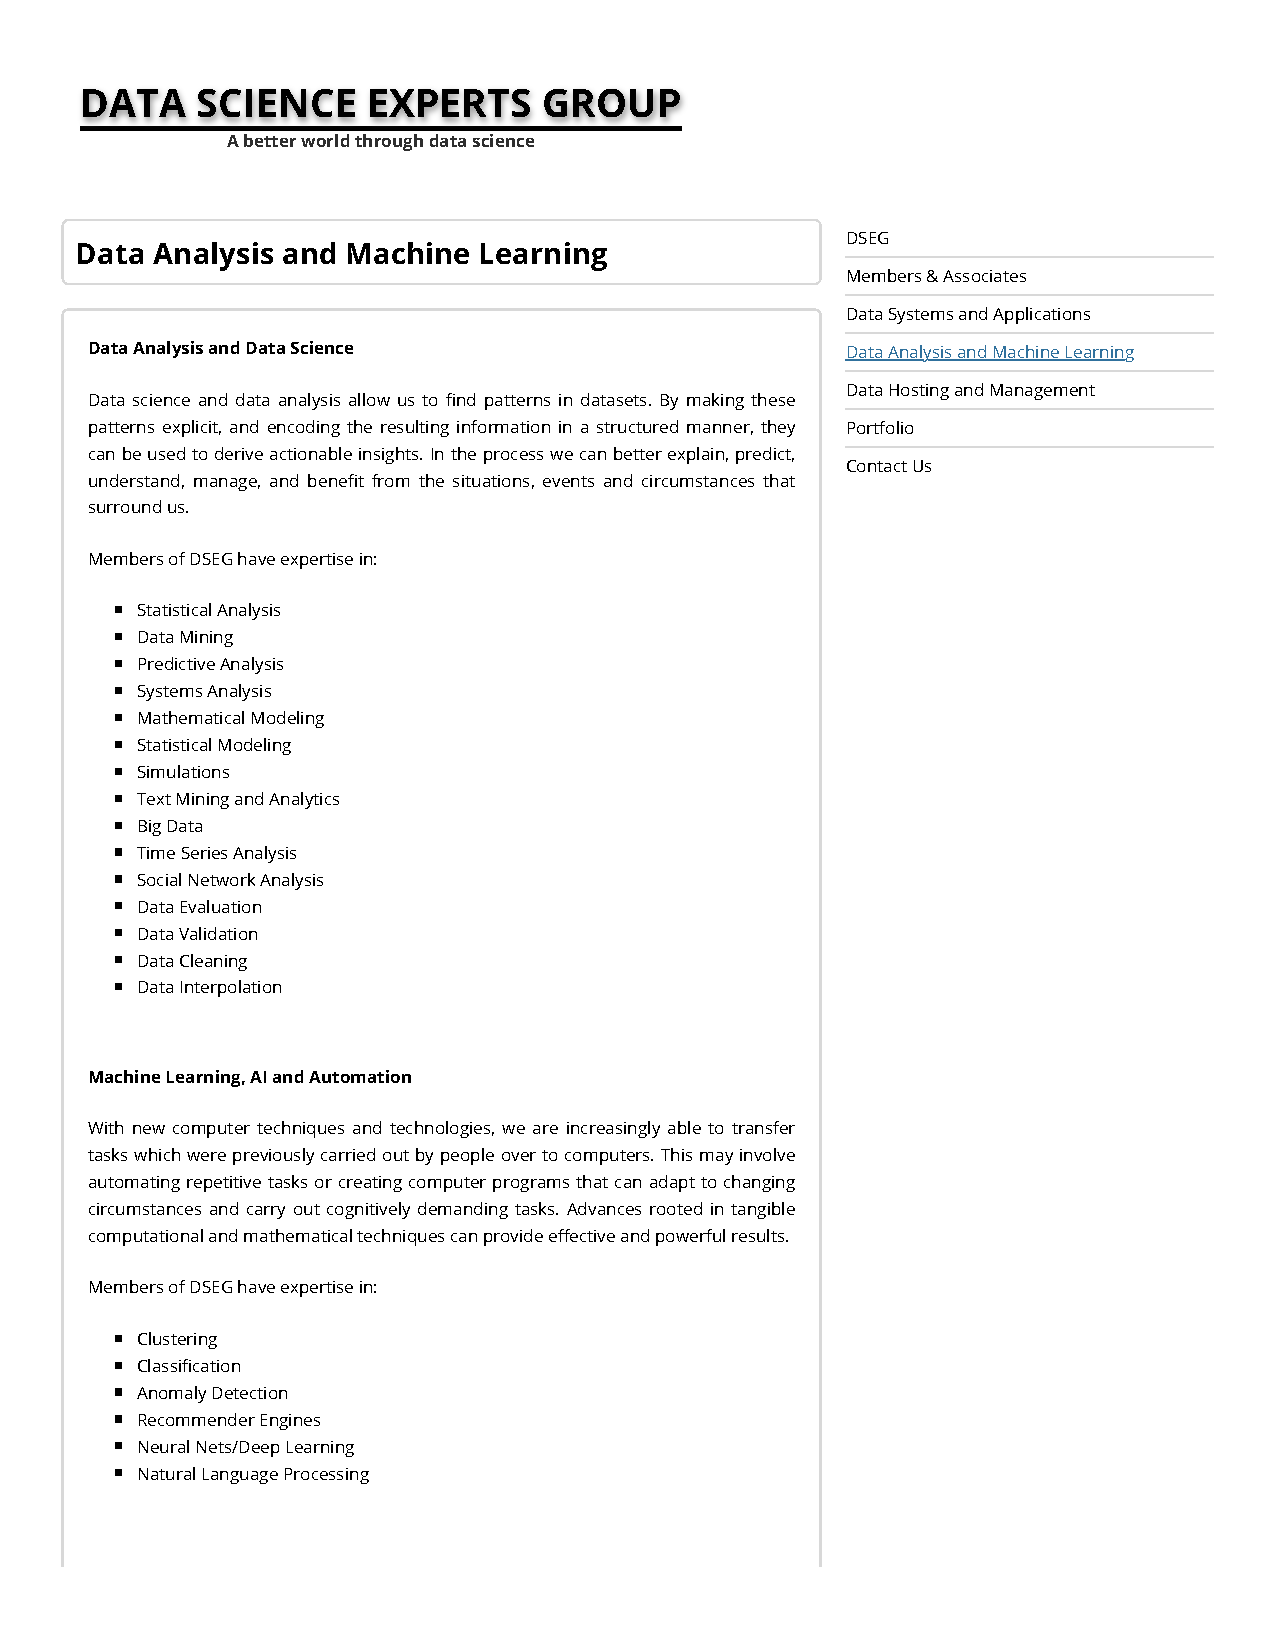
\includepdf[pages={1},offset={50 -40}]{documents/DSEG4.pdf}
 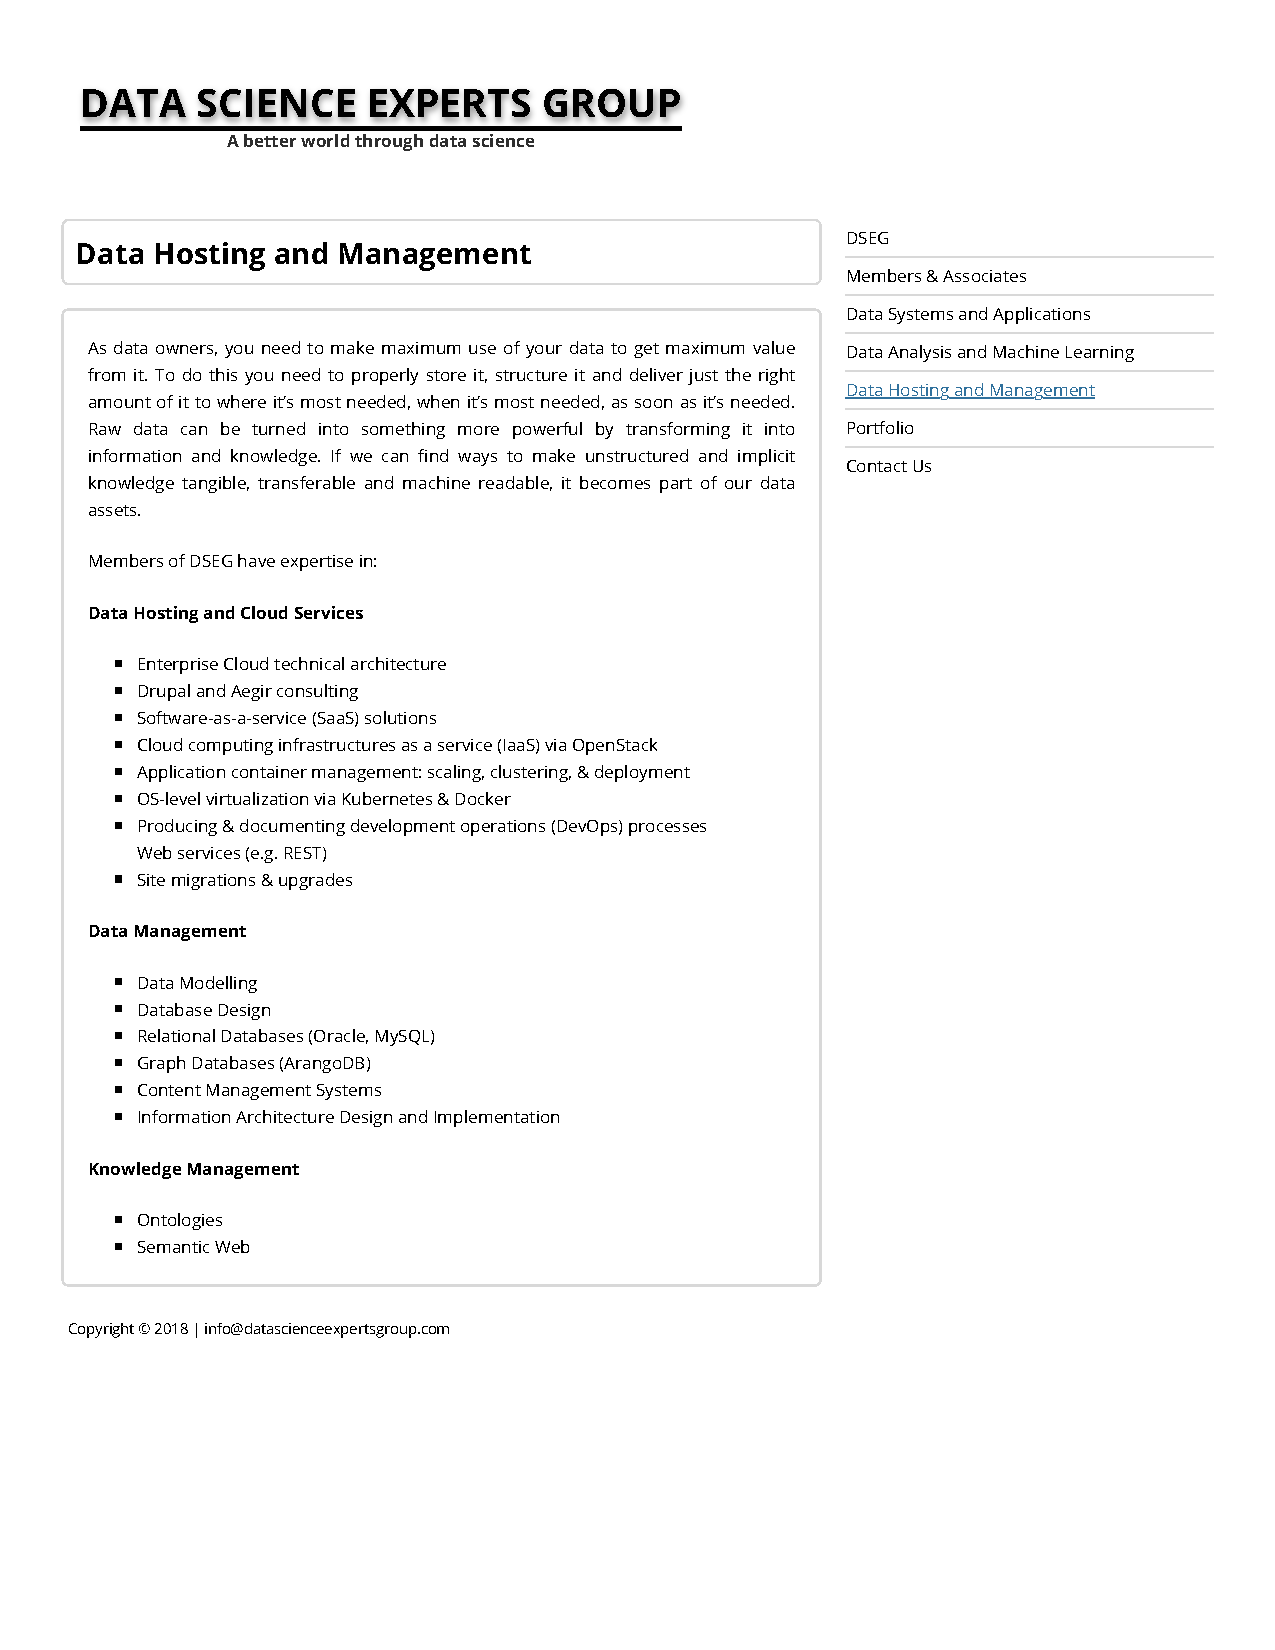
\includepdf[pages={1},offset={50 -40}]{documents/DSEG5.pdf}
 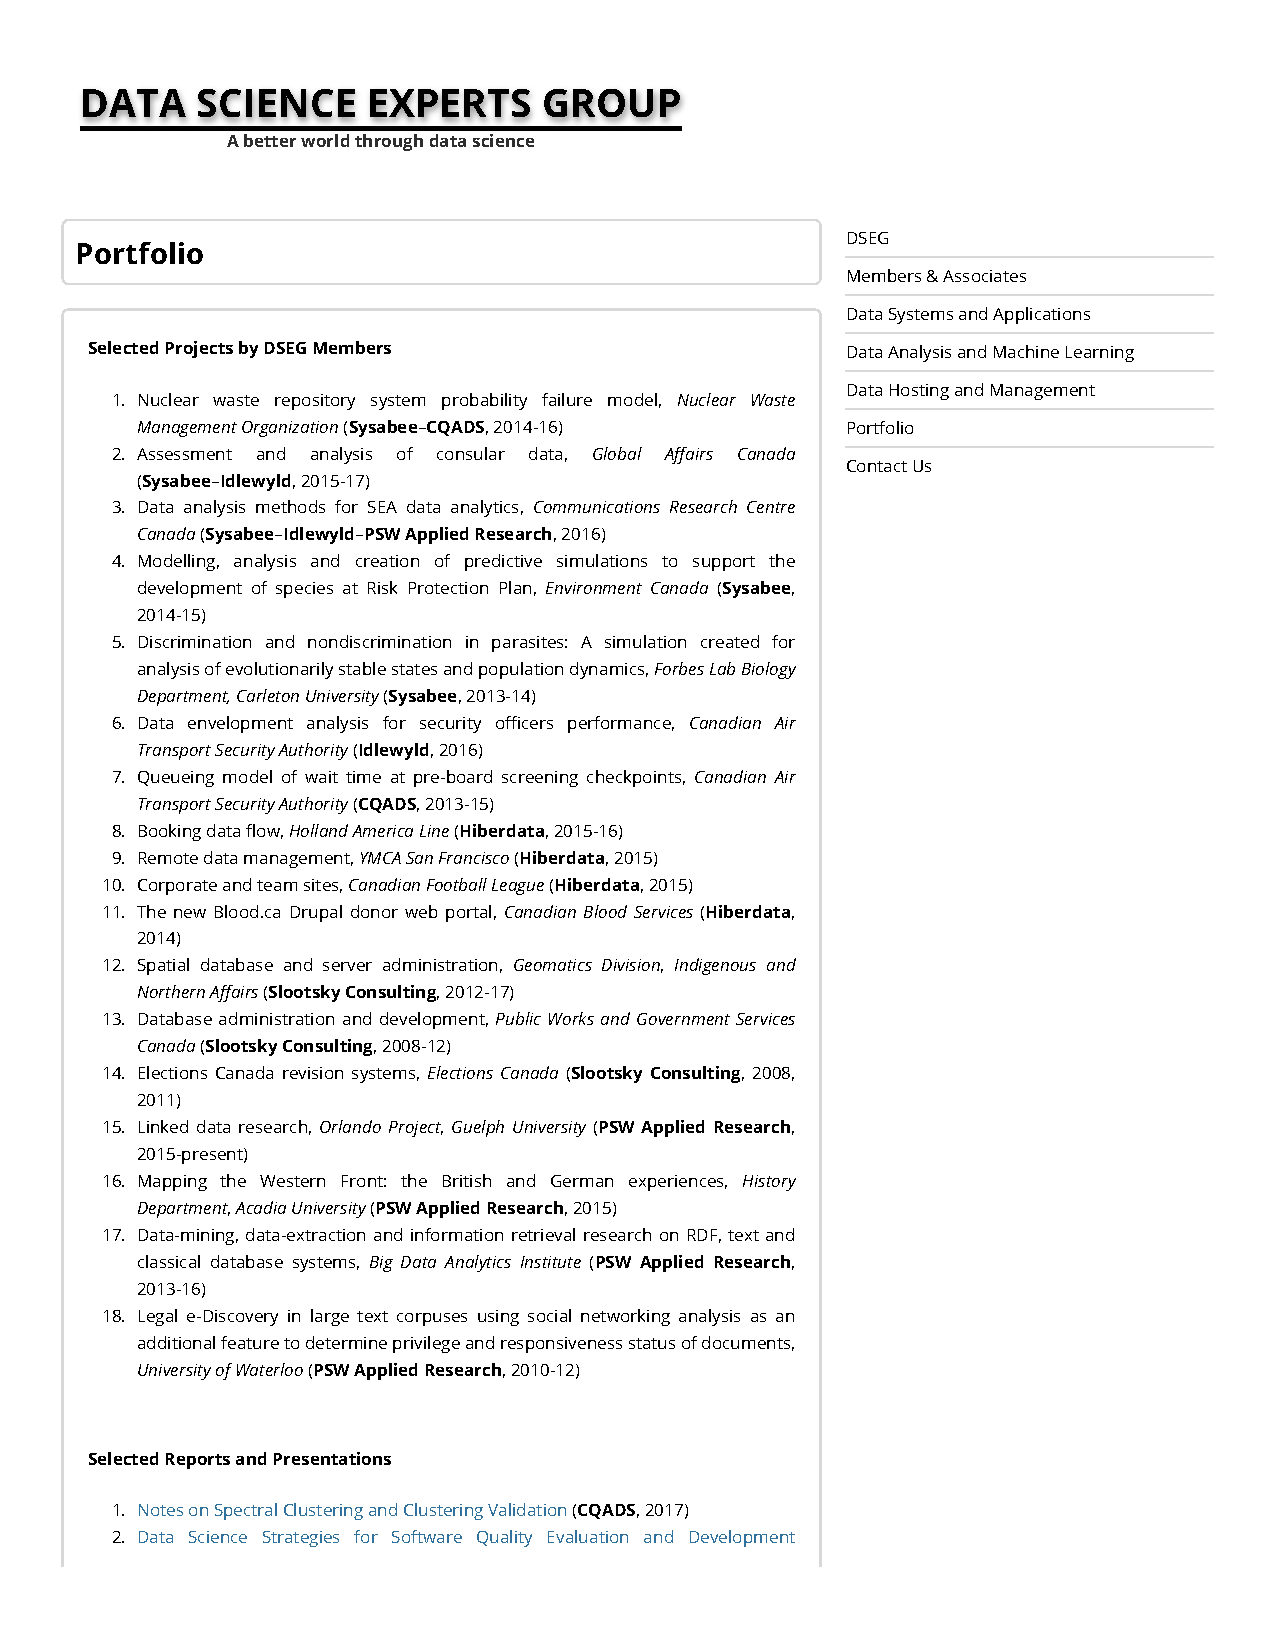
\includepdf[pages={1},offset={50 -40}]{documents/DSEG6.pdf}
 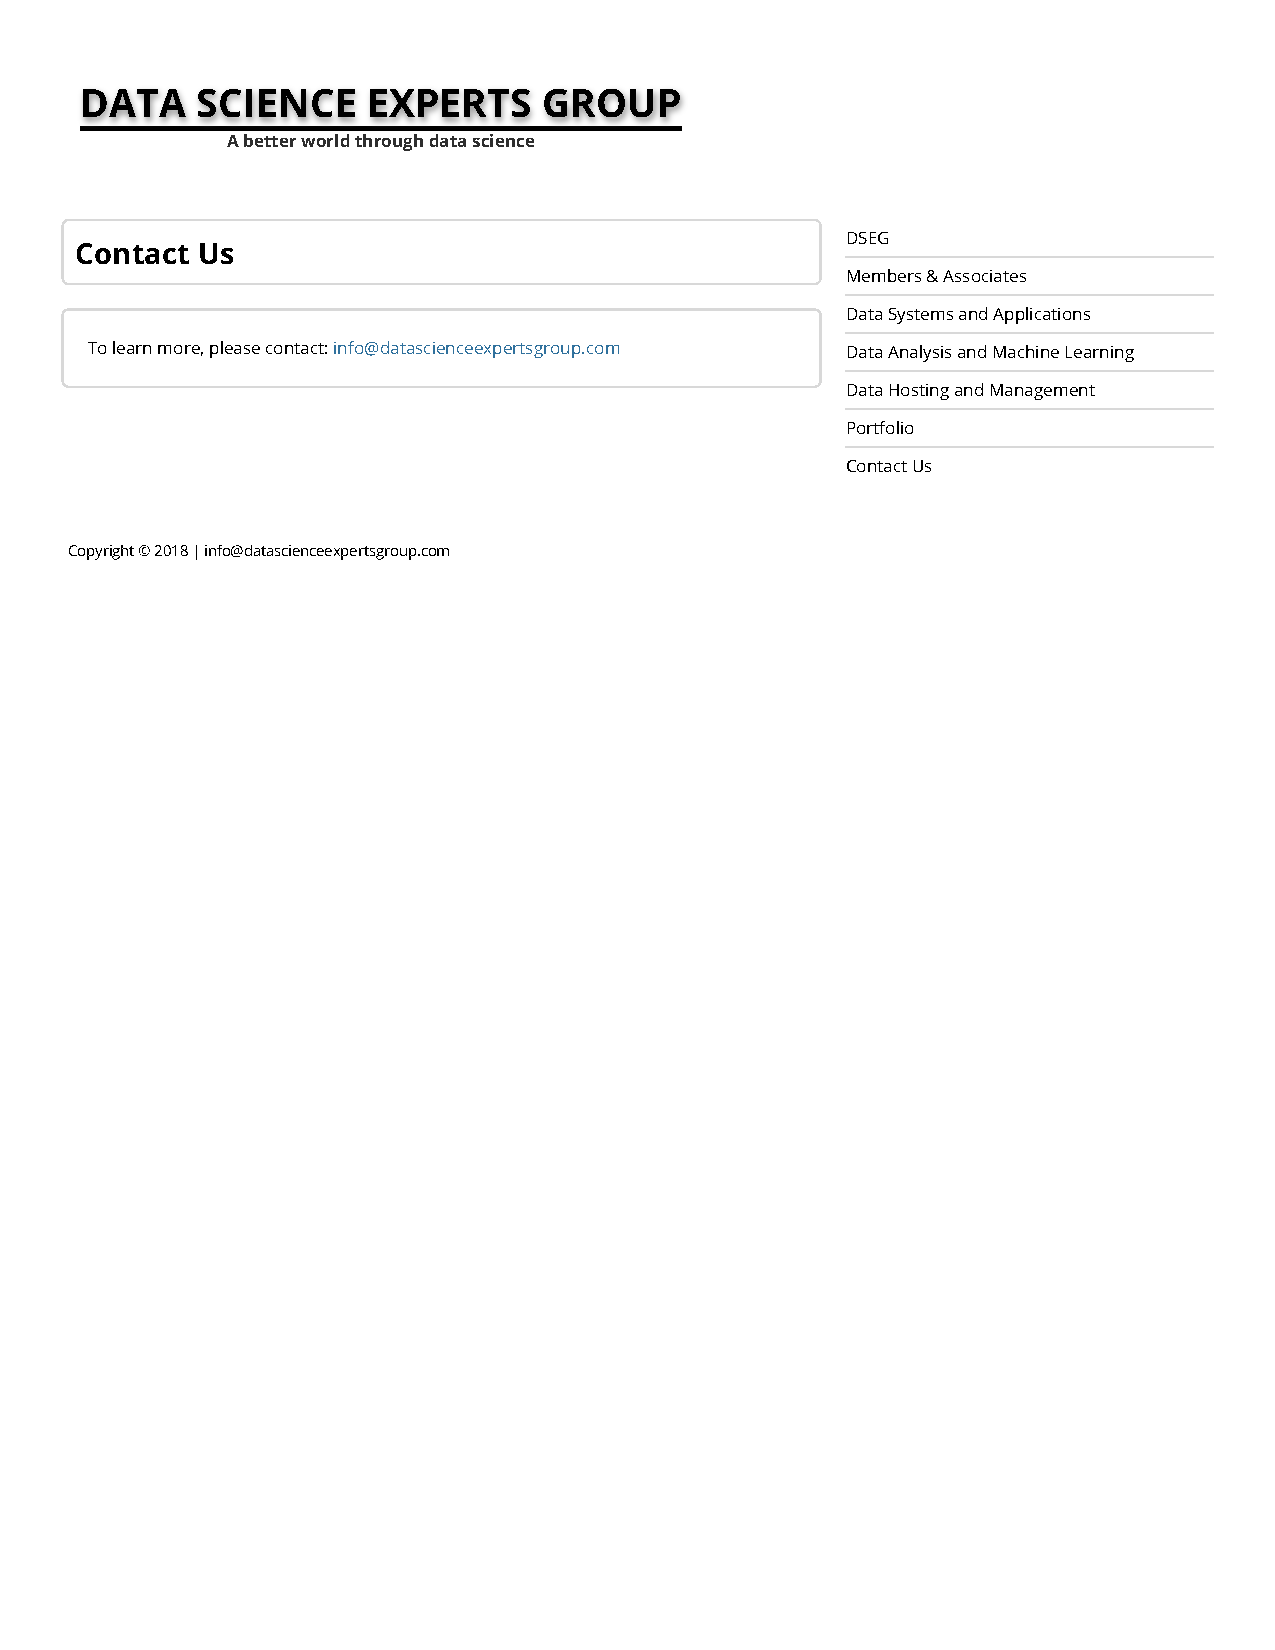
\includepdf[pages={1},offset={50 -40}]{documents/DSEG7.pdf}
 \addtocounter{subsubsection}{1}
 \addcontentsline{toc}{subsubsection}{\protect\numberline{\thesubsubsection}Blogs and White Papers}
 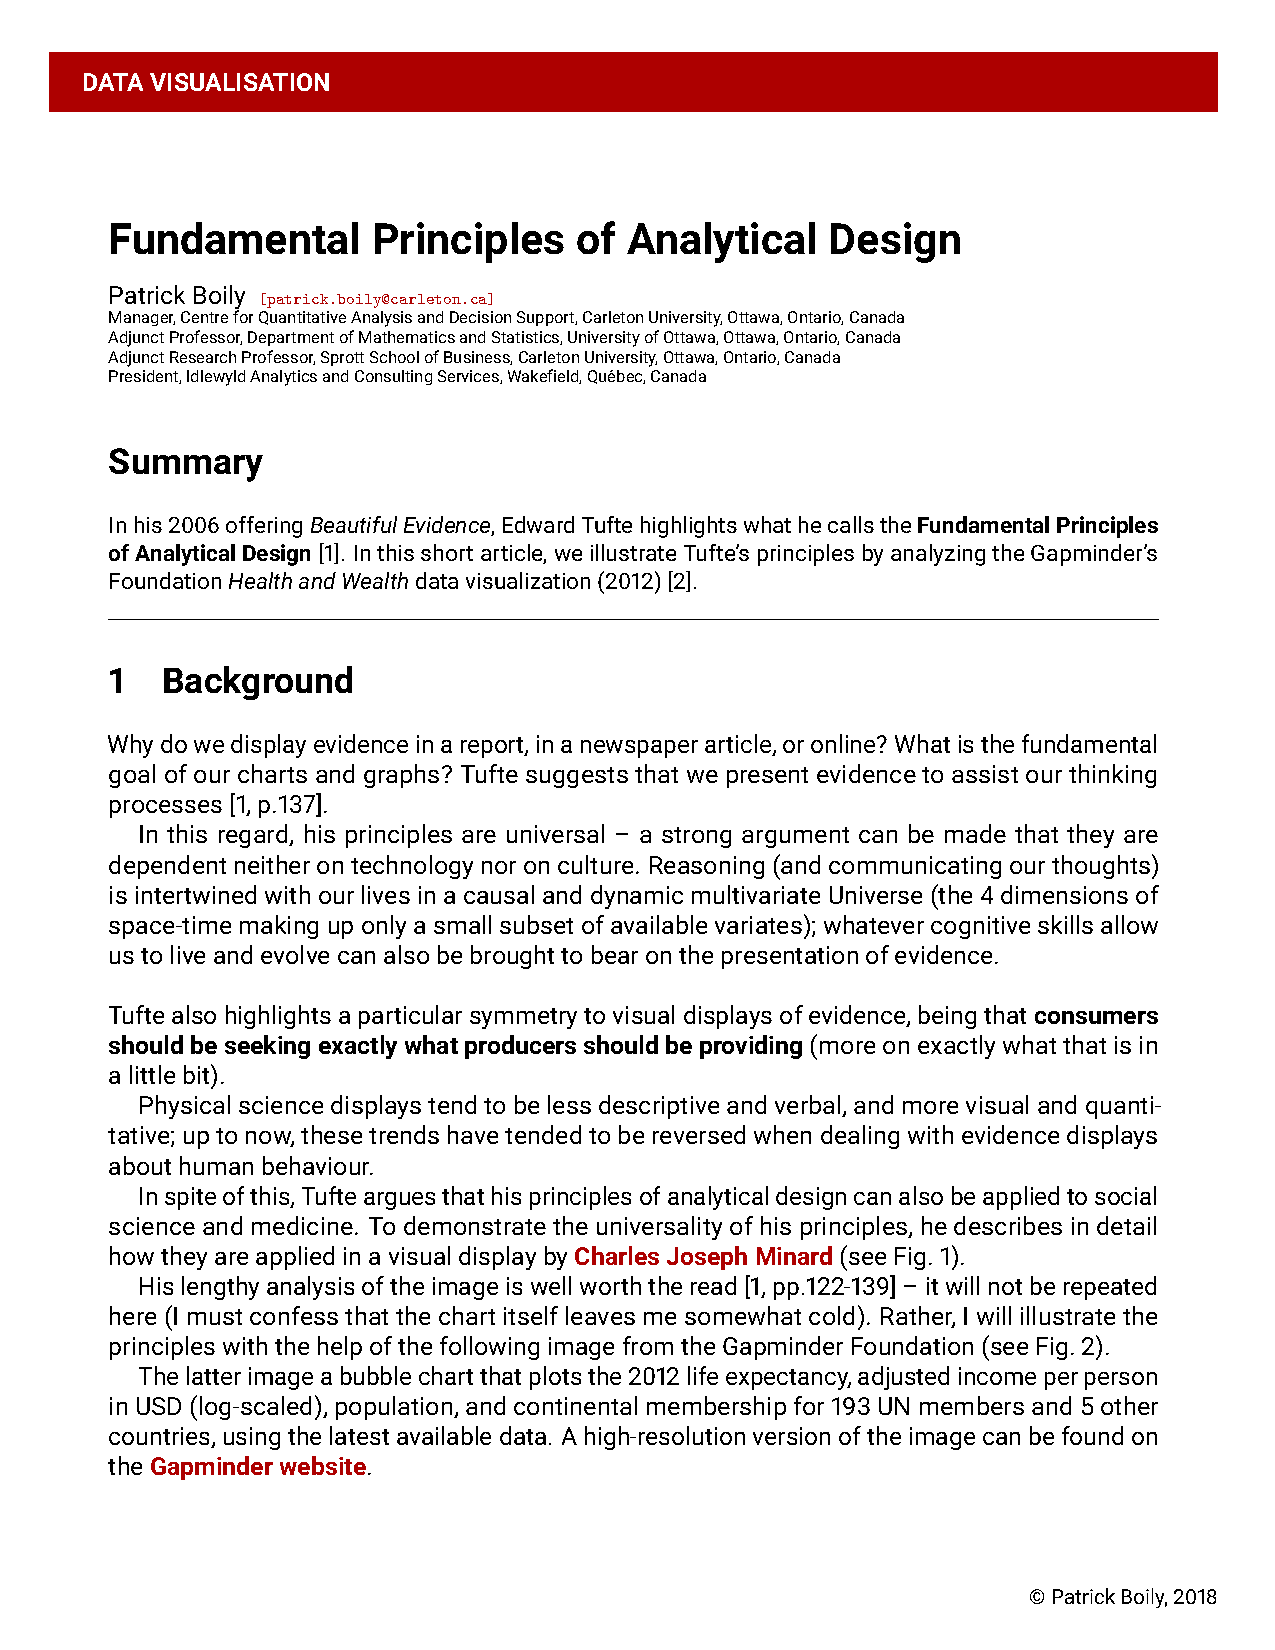
\includepdf[pages={1-16},offset={50 -40}]{documents/TFPD.pdf}
\addtocounter{subsubsection}{1}
 \addtocounter{subsubsection}{1}
 \addcontentsline{toc}{subsubsection}{\protect\numberline{\thesubsubsection}Jupyter Notebooks}
 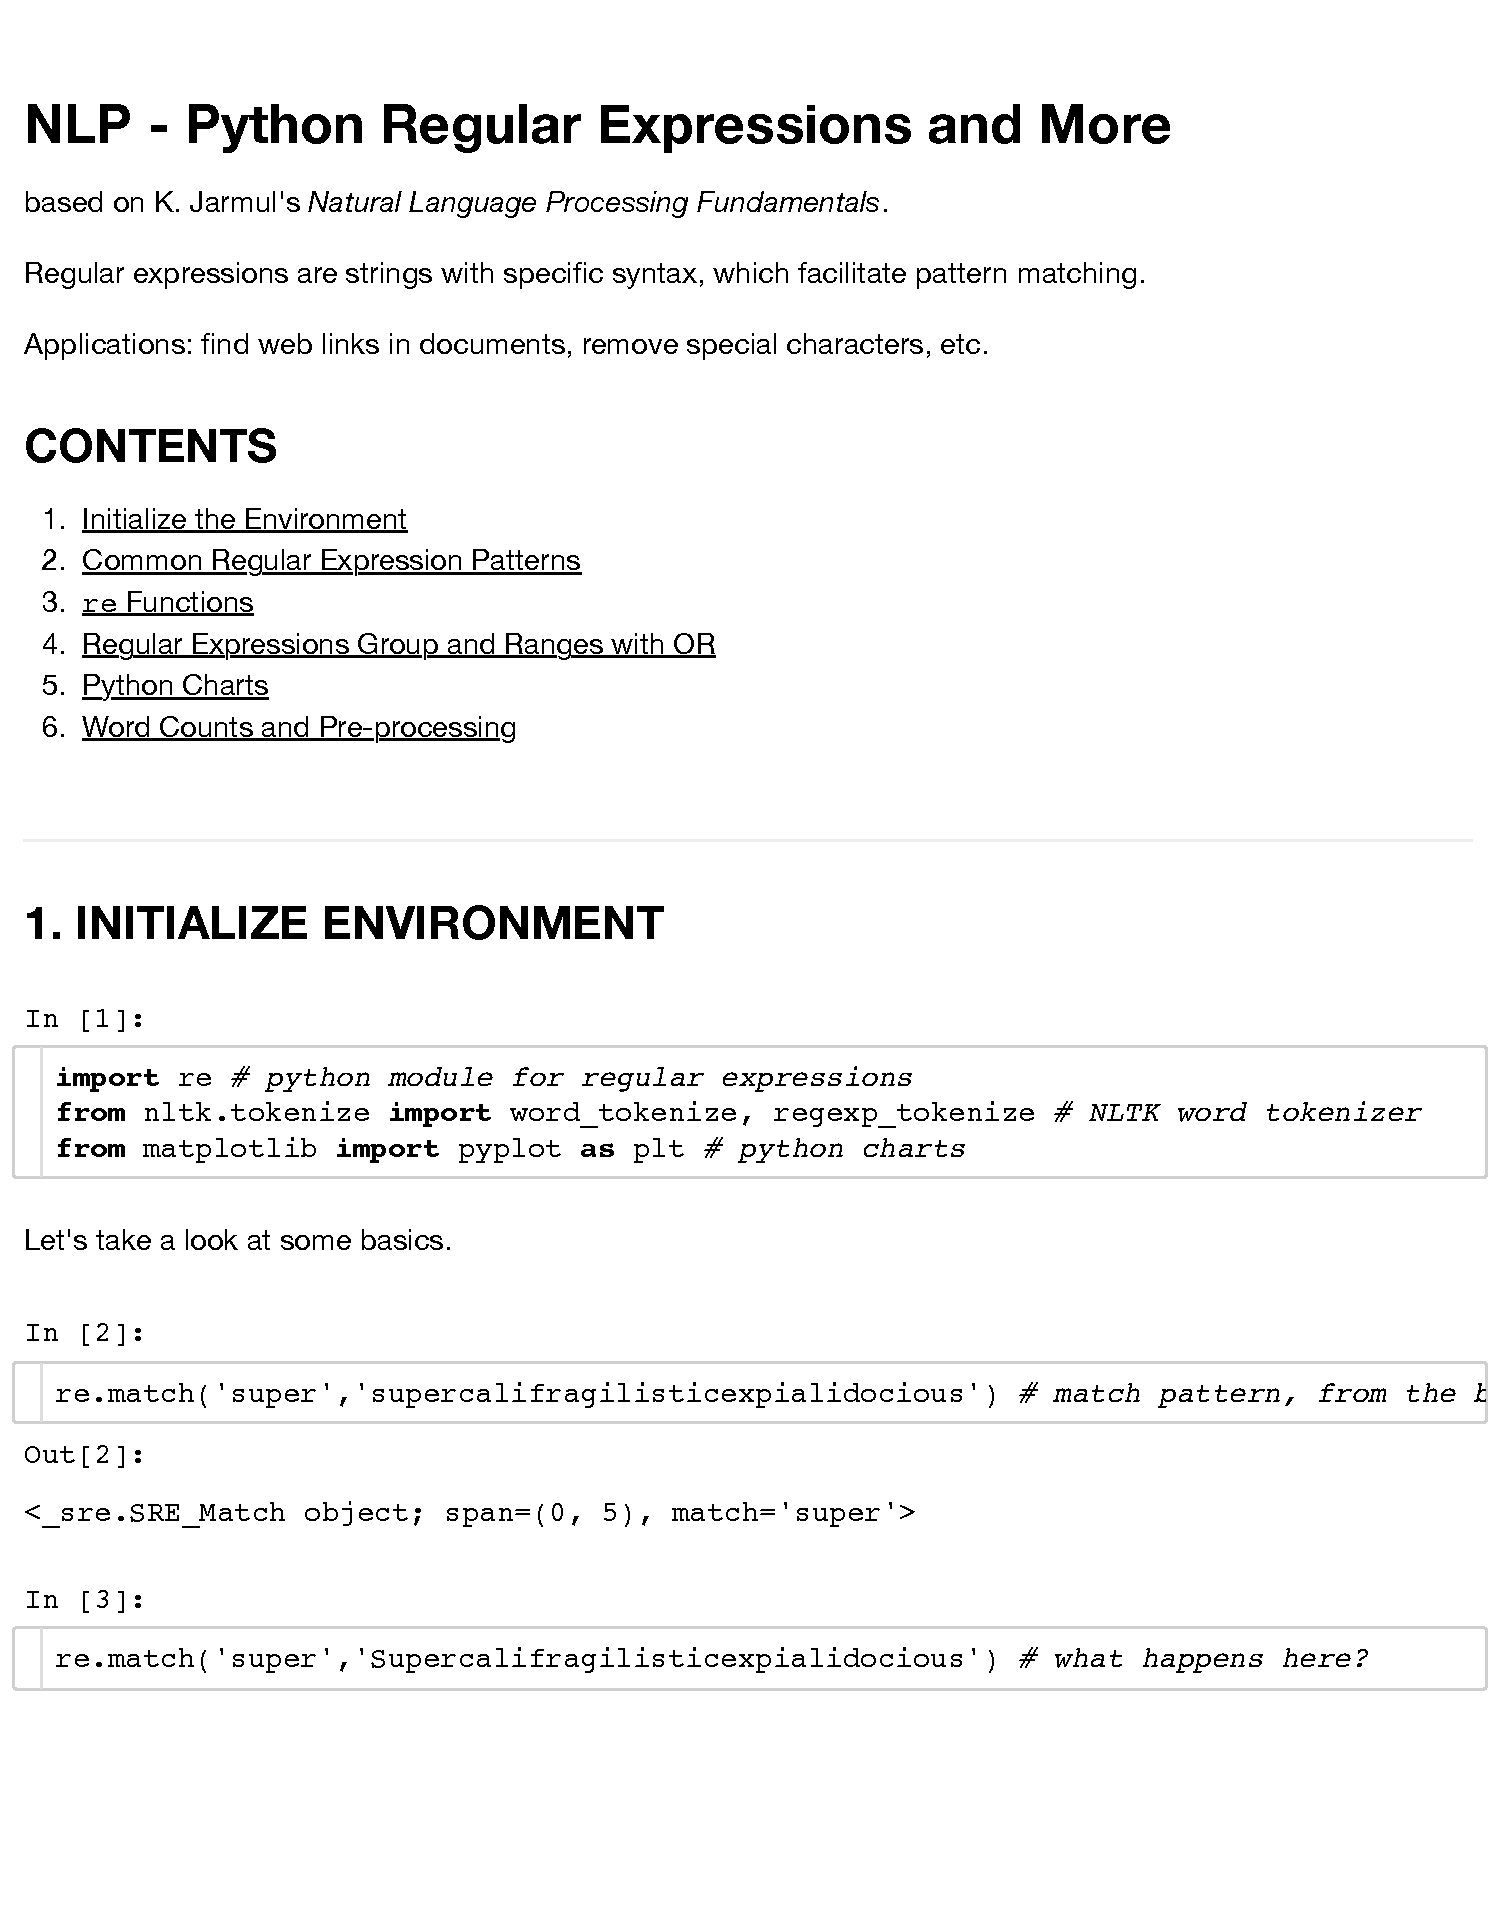
\includepdf[pages={1-9},offset={50 -40}]{documents/Python_Regular_Expressions_and_More.pdf}
\addtocounter{subsubsection}{1}
\addcontentsline{toc}{subsubsection}{\protect\numberline{\thesubsubsection}Proposals}
 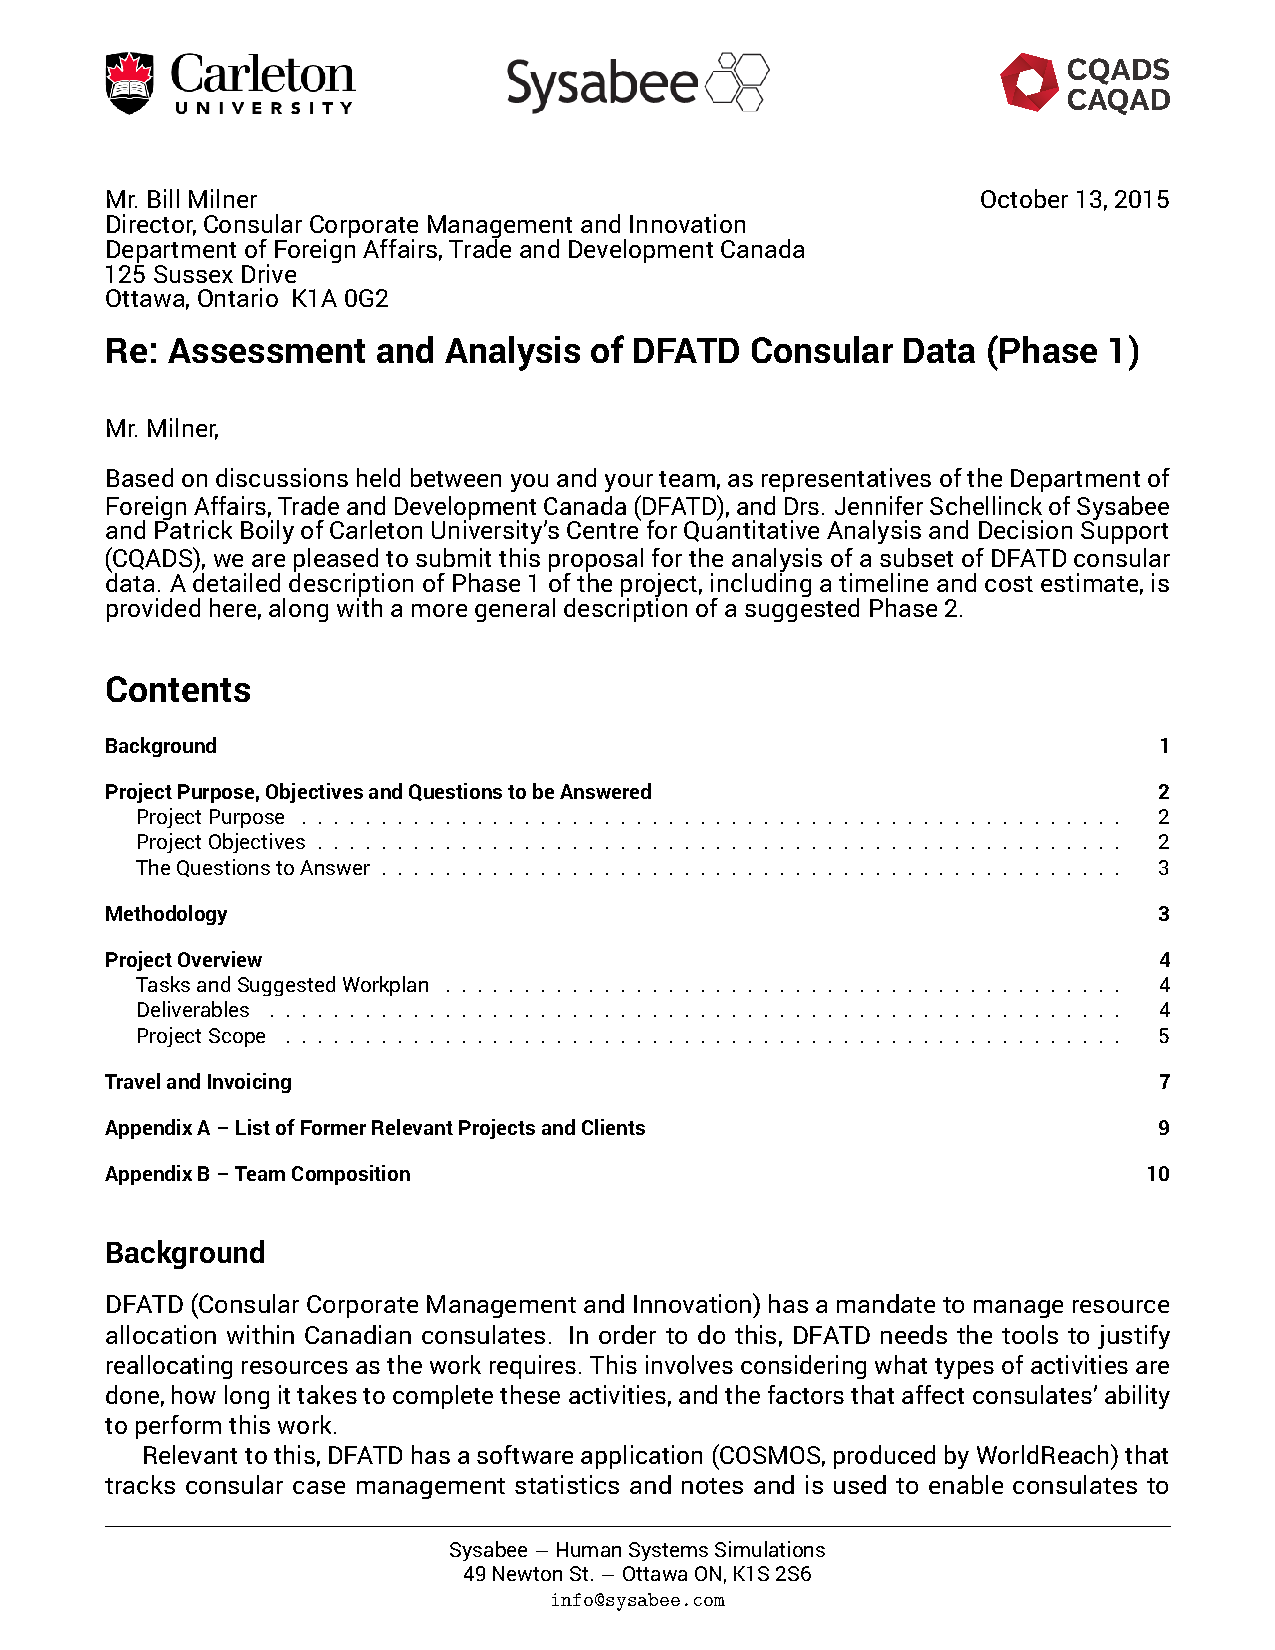
\includepdf[pages={1-7,9-10},offset={50 -40}]{documents/Pr_GAC1.pdf}
 
\includepdf[pages={1-3},offset={50 -40}]{documents/Pr_GAC2.pdf}
 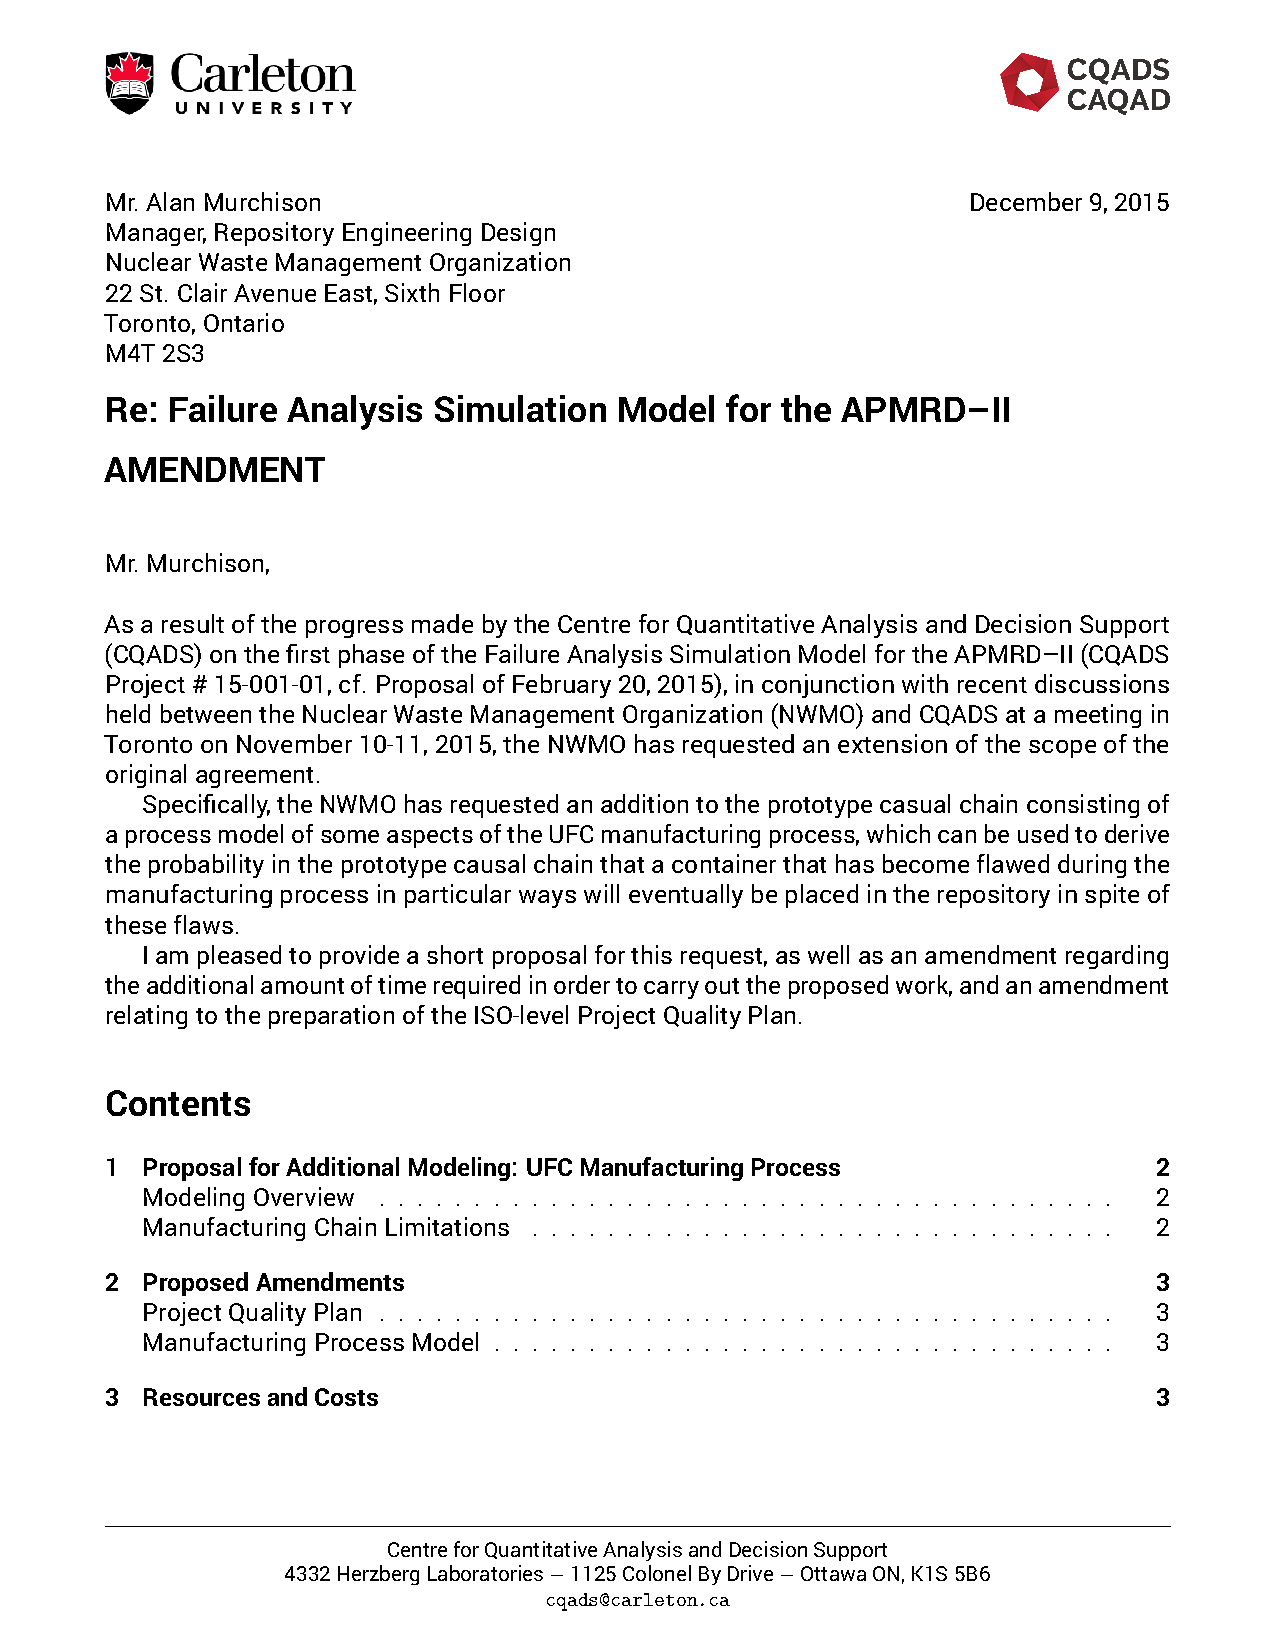
\includepdf[pages={1-4},offset={50 -40}]{documents/Pr_NWMO_Amendment.pdf}
 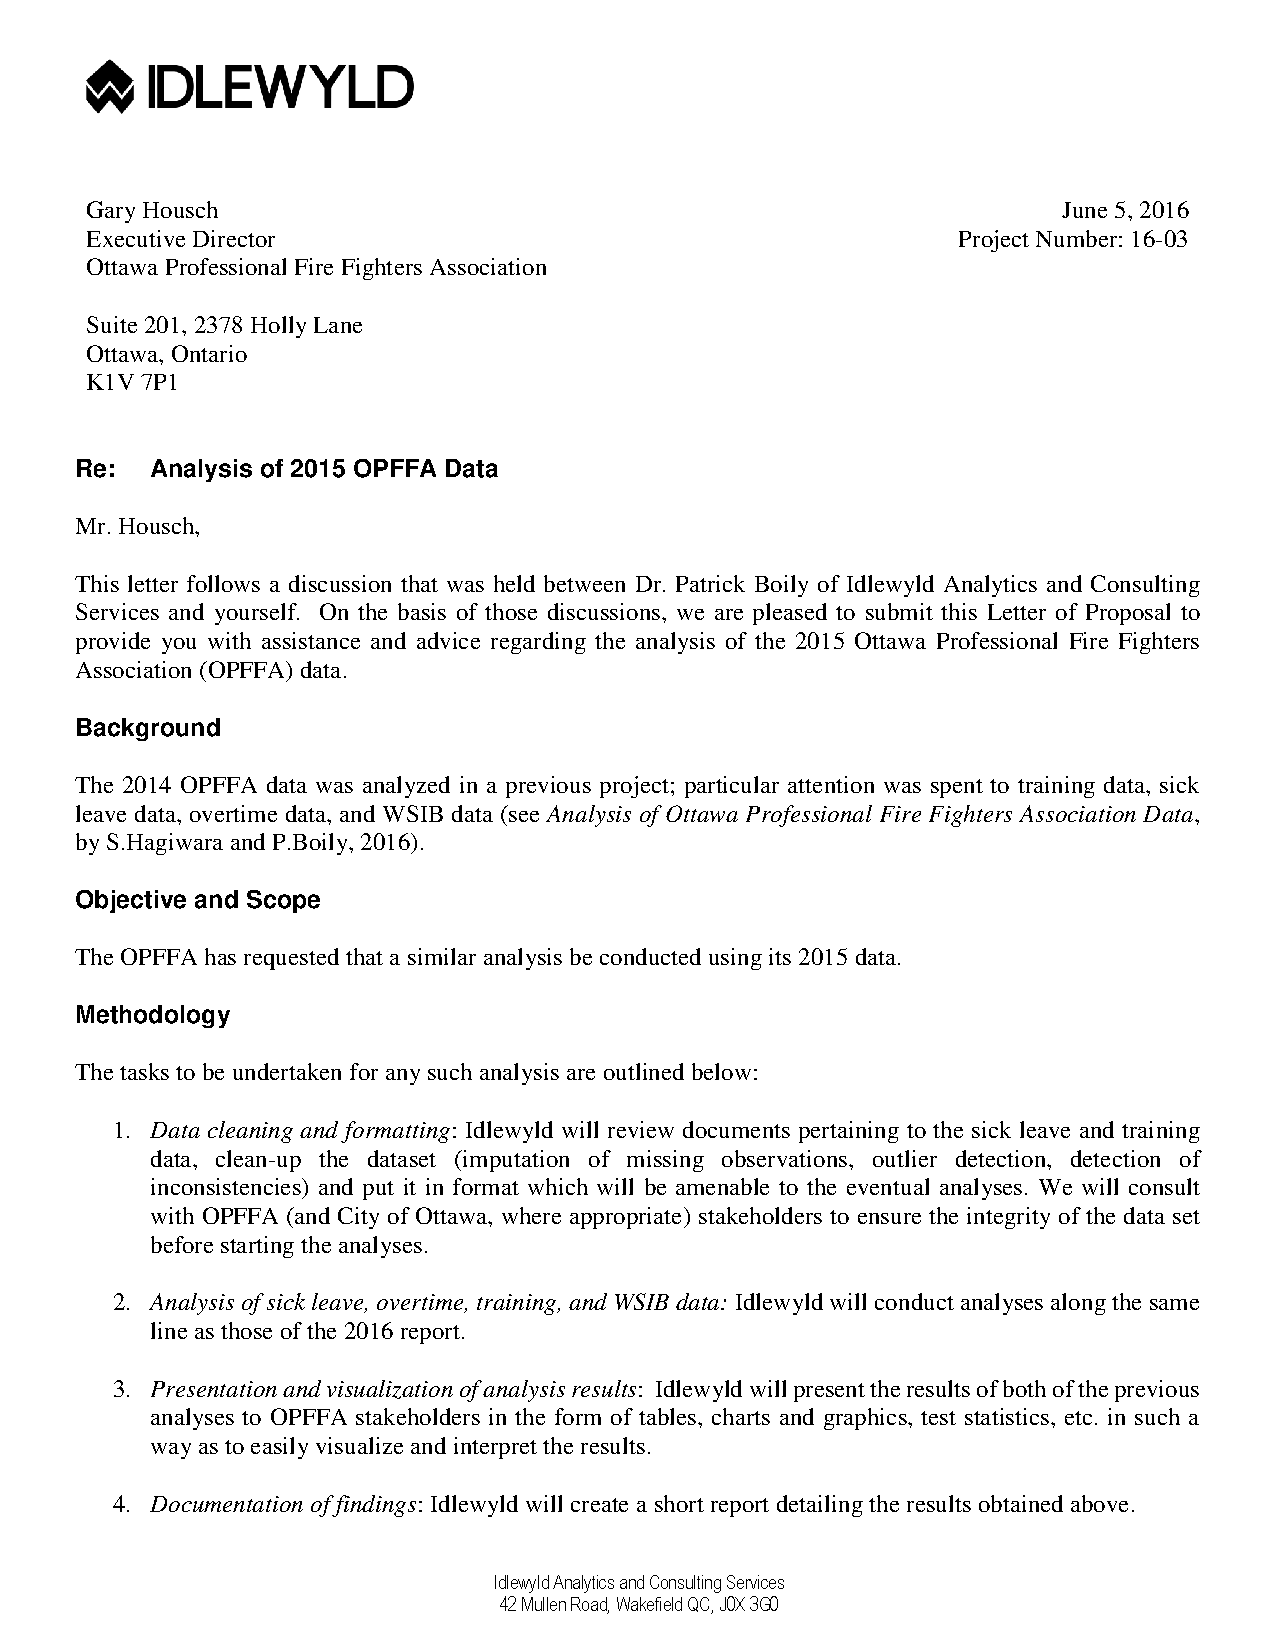
\includepdf[pages={1-3},offset={50 -40}]{documents/Pr_OPFFA2.pdf}
 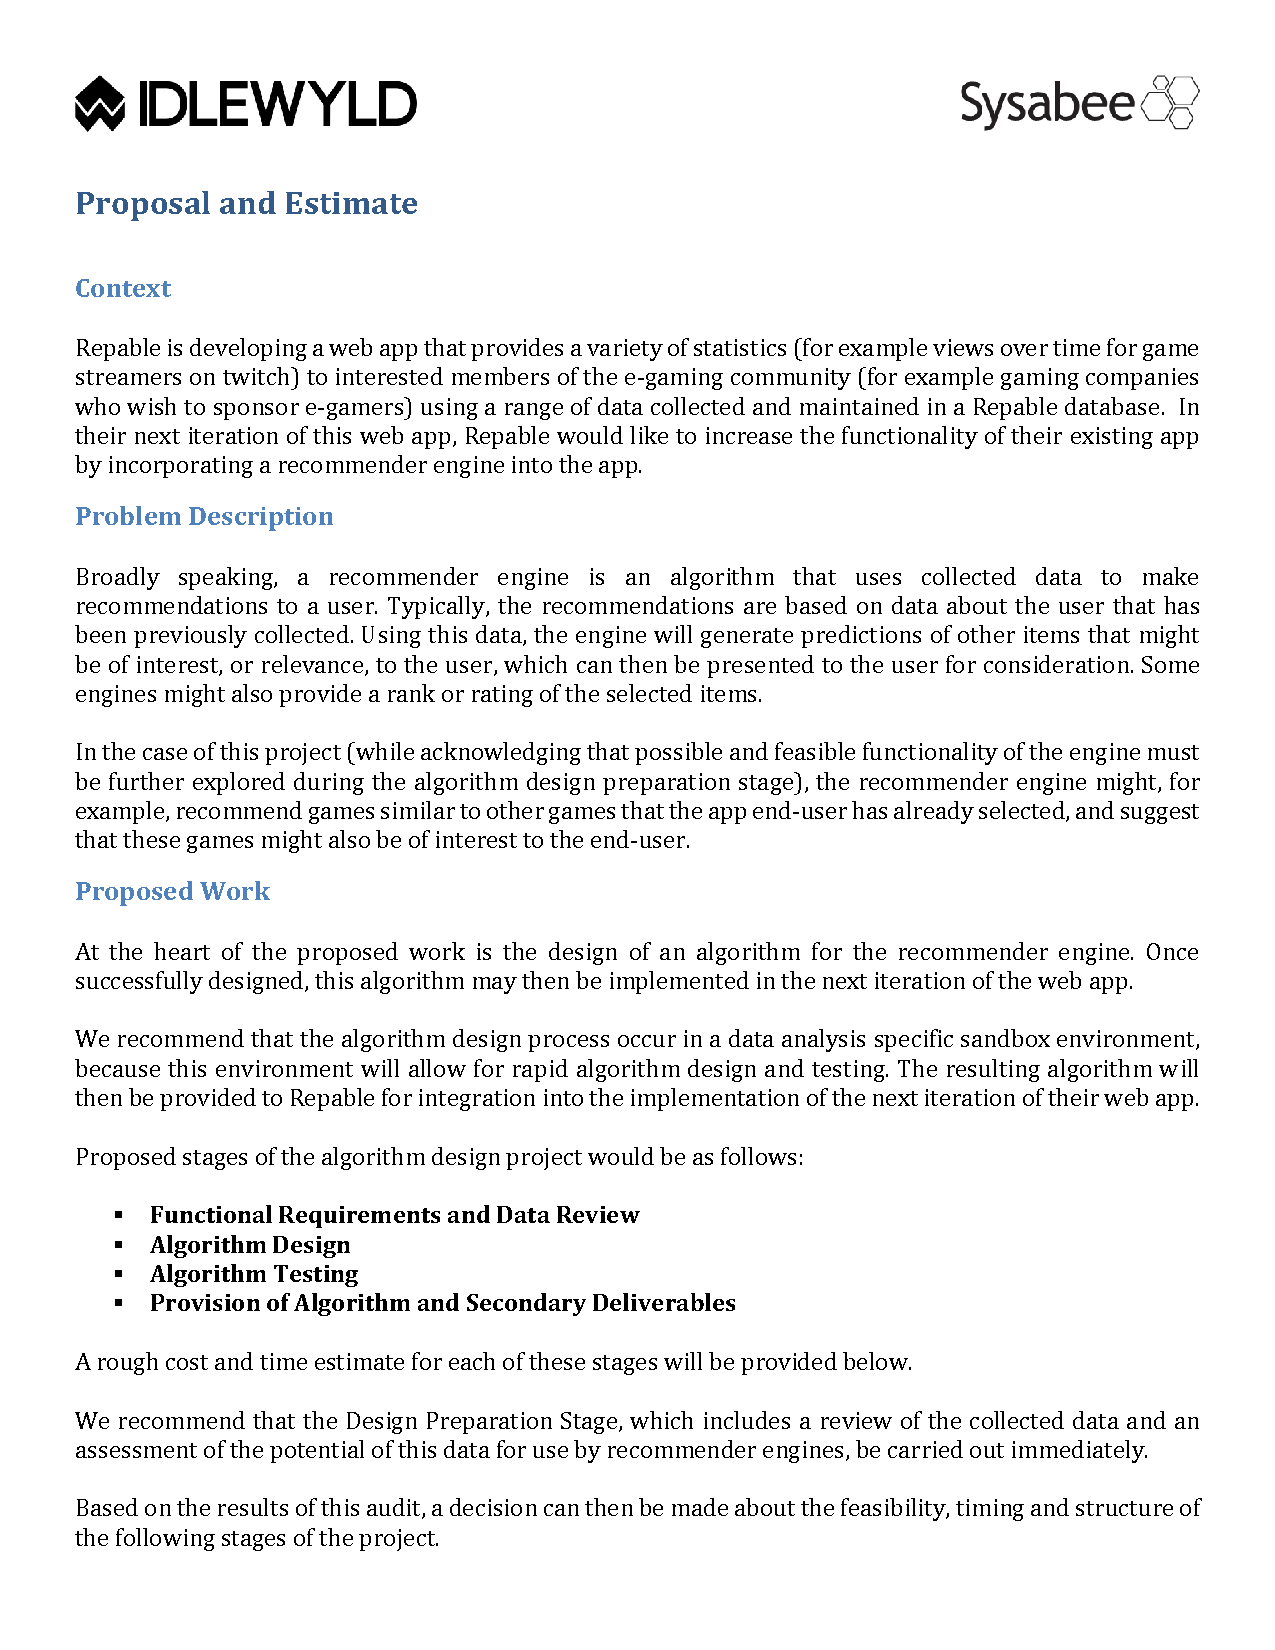
\includepdf[pages={1-2},offset={50 -40}]{documents/Pr_Repable.pdf} 
\addtocounter{subsubsection}{1}
\addcontentsline{toc}{subsubsection}{\protect\numberline{\thesubsubsection}Quality Plans}
 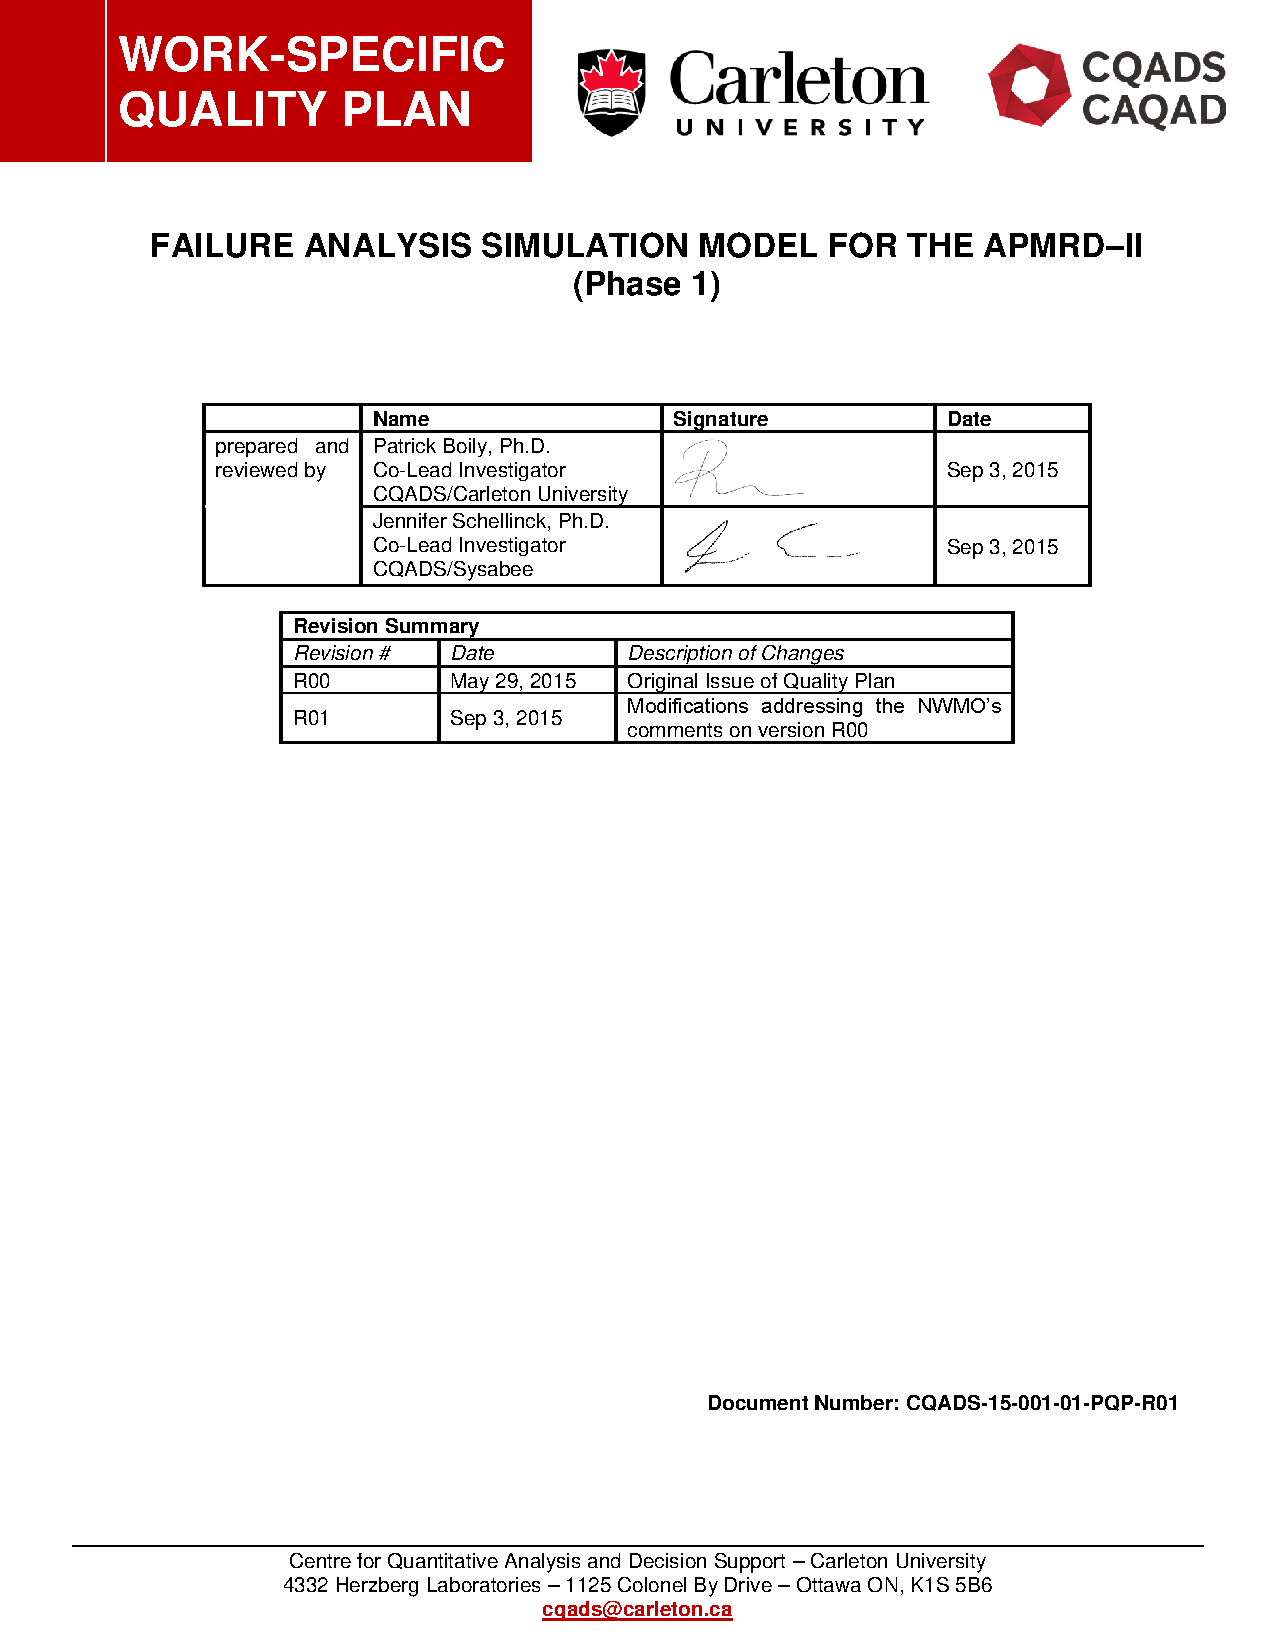
\includepdf[pages={1-22},offset={50 -40}]{documents/PQPNWMO.pdf}
 \addtocounter{subsubsection}{1}
\addcontentsline{toc}{subsubsection}{\protect\numberline{\thesubsubsection}Progress Reports}
 
\includepdf[pages={1-4},offset={50 -40}]{documents/PR_NWMO1.pdf}
 \includepdf[pages={1-4},offset={50 -40}]{documents/PR_NWMO2.pdf}
 \includepdf[pages={1-4},offset={50 -40}]{documents/PR_NWMO3.pdf}
\setboolean{@twoside}{true}
 \addtocounter{subsubsection}{1}
 \addcontentsline{toc}{subsubsection}{\protect\numberline{\thesubsubsection}Project Planning}
\includegraphics[width=\textwidth]{documents/Phases.png}
\includegraphics[width=\textwidth]{documents/Phases1Tasks.png}
\begin{landscape}
\includegraphics[width=\textheight]{documents/Tasks_1.png}
\includegraphics[width=\textheight]{documents/Tasks_2.png}
\includegraphics[width=\textheight]{documents/Tasks_3.png}
\end{landscape}


%\section{Technical Requirements}
\newpage\subsection{Programming}
\paragraph{Open Source Coding}
\paragraph{Commercial Packages}
\paragraph{Notes and Comments}\afterpage{\FloatBarrier}
\newpage\section{Data Management and Pipelines}
\subsection{Data Modeling}
\subsection{Data Storage and Access}
\subsection{Pipelines}
\subsection{Data Wrangling}
\afterpage{\FloatBarrier}
%\newpage\input{sections/sub_Data_Wrangling.tex}\afterpage{\FloatBarrier}
\section{Survey of Quantitative Methods}
 The bread and butter of quantitative consulting is the ability to apply quantitative methods to business problems in order to obtain actionable insight. Clearly, it is impossible (and perhaps inadvisable, in a more general sense) for any given individual to have expertise in every field of mathematics, statistics, and computer science. \par We believe that the best consulting framework is reached when a small team of consultants possesses expertise in 2 or 3 areas, as well as a decent understanding of related disciplines, and a passing knowledge in a variety of other domains: this includes keeping up with trends, implementing knowledge redundancies on the team, being conversant in non-expertise areas, and knowing where to find detailed information (online, in books, or through external resources). \newl In this section, we present an introduction for 9 ``domains'' of quantitative analysis:
\begin{itemize}[noitemsep]
\item survey sampling and data collection;
\item data processing;
\item data visualisation;
\item statistical methods;
\item queueing models;
\item data science and machine learning;
\item simulations;
\item optimisation, and
\item trend extraction and forecasting;
\end{itemize}
Strictly speaking, the domains are not free of overlaps. Large swaths of data science and time series analysis methods are quite simply statistical in nature, and it's not unusual to view optimisation methods and queueing models as sub-disciplines of operations research. Other topics could also have been included (such as Bayesian data analysis or signal processing, to name but two), and might find their way into a second edition of this book. 
\par Our treatment of these topics, by design, is brief and incomplete. Each module is directed at students who have a background in other quantitative methods, but not necessarily in the topic under consideration. Our goal is to provide a quick ``reference map'' of the field, together with a general idea of its challenges and common traps, in order to highlight opportunities for application in a consulting context. These subsections are emphatically NOT meant as comprehensive surveys: they focus on the basics and talking points; perhaps more importantly, a copious number of references are also provided. \par We will complement each section with projects projects we have tackled in our own practices. These case studies are accompanied by (partial) deliverables in the form of charts, write-ups, report extract, etc.). 
\begin{center}
    \rule{0.5\textwidth}{.4pt}
\end{center}
As a final note, we would like to stress the following: it is \textbf{IMPERATIVE} that quantitative consultants remember that acceptable business solutions are not always optimal theoretical solutions. Rigour, while encouraged, often must take a backseat to applicability. This lesson can be difficult to accept, and has been the downfall of many a promising candidate.  
%\subsection{Motivating Examples}
%\begin{itemize}
%\item Various federal departments are looking to produce national and sub-national estimates for a number of vehicle-use statistics (vehicle-km traveled, fuel consumption, idling time, etc.). What's the best way to obtain these estimates?  
%\item The \textit{National Collision Database} contains information about motorists and pedestrians involved in collisions in Canada, as well as information about the collision itself. In a fatal collision, the blood alcohol content levels cannot be obtained until after the coroner's report is available, which can take up to a year. Can we predict the missing BAC in the meantime?    
%\item The \textit{Ottawa Professional Fire Fighters Association} represents the interests of fire fighters in the City, which is pushing to reduce the number of sick leave hours to a pre-determined benchmark. Is this plan attainable? Similarly, the city has requested that three hours of training must be scheduled and logged into a computer for each twenty-four hour shift. While there is some evidence that employees are participating in increased amounts of training, the \textit{Record Management System} (RMS) suggests that such training experience is in fact decreasing. Can we determine if there are errors in the RMS numbers, or if the evidence is biased?
%\item \textit{Global Affairs Canada} (GAC) uses various tools to track the time required by employees to perform consular tasks abroad. This data stretches back over approximately twenty years. This system, and the data it collects, are used to determine the effectiveness of mission consular programs, identify weaknesses to be resolved through HR, training and other solutions, and is used to evaluate the need for resources in missions. It is in fact the pivotal element when determining whether to staff, delete, or create positions. The software is in the process of being updated/replaced. As part of this process, GAC is generating software requirements to ensure that the updated system collects accurate and relevant data, while continuing to carry out data analyses that support mission resource use management. In preparation for this update,  GAC would like to know how to implement a data collection system that will collect accurate, usable data that allows for resource use evaluation on a mission by mission basis; what data collection functionality would be required to support the use of more advanced data analysis and modeling techniques; which collected mission attributes allow for accurate assessments of missions resource use; which missions can be appropriately grouped together when evaluating mission effectiveness and efficiency (`apples to apples' comparisons). Is this feasible? 
%\item STO UNION
%\item CCNM
%\item Repable
%\item PHAC - CIS
%\item PHAC - other
%\item Nordicity
%\item CATSA - DEA
%\item CATSA - Association Rules
%\item CATSA - Queueing
%\item NWMO
%\item UWCC
%\item WBNP
%\item Bayne Sellar Boxall
%\item CAZA
%\item CMHC
%\item Commission for Public Complaints against the RCMP
%\item CRCC
%\item Synchro Canada
%\item TC - Multimodal
%\item Corrections Canada
%\item Foodicus
%\end{itemize}

%\newpage\subsection{Principles of Data Collection} \label{sec:DC}
\begin{tcolorbox}[title=Fisher's Maxim]
To consult the statistician after an experiment is finished is often merely to ask him to conduct a post mortem examination. He can perhaps say what the experiment died of. \\[-0.6cm]
\begin{flushright}
-- R.A. Fisher, Presidential Address to the \textit{First Indian Statistical Congress}, 1938
\end{flushright}
\end{tcolorbox}
\noindent Data analysis tools and techniques work in conjunction with collected data. The type of data that needs to be collected to carry out such analyses, as well as the priority placed on the collection of quality data relative to other demands, will dictate the choice of data collection strategies. The manner in which the resulting outputs of these analyses are used for decision support will, in turn, influence appropriate data presentation strategies and system functionality (we will revisit this aspect in a later section).  
\newl Although consultants should always endeavour to work with \textbf{representative} and \textbf{unbiased data}, there will be times when the available data is flawed and not easily repaired. Quantitative consultants have a professional responsibility to explore the data, looking for potential fatal flaws \textbf{prior} to  the start of the analysis and to inform their client of any findings that could halt, skew, or simply hinder the analytical process or its applicability to the situation at hand. 
\par Unless a clause has specifically been put in the contract to allow a graceful exit at this point, you will have to proceed with the analysis, flaws and all. It is  \textbf{EXTREMELY IMPORTANT} that you do not simply sweep these flaws under the carpet. Address them repeatedly in your meetings with the clients, and make sure that  the analysis results you present or report on include an appropriate \textit{caveat}. \paragraph{Data Collection System} Consultants might also be called upon to provide suggestions to evaluate or fix the data collection system. The following items could help with that task. 
\begin{itemize}[noitemsep]
\item \textbf{Data Validity}: the system must collect the data in such a way that data validity is ensured during initial collection. In particular, data must be collected in a way that ensures sufficient accuracy and precision of the data, relative to its intended use.
\item \textbf{Data Granularity, Scale of Data}: the system must collect the data at a level of granularity appropriate for future analysis.
\item \textbf{Data Coverage}: the system must collect data that comprehensively, rather than only partially or unevenly, represents the objects of interest. As well, the system must collect and store the required data over a sufficient amount of time, and at the required intervals, to support data analyses that require data spanning a certain duration.
\item \textbf{Data Storage}: the system must have the functionality to store the types and amount of data required for a particular analysis.
\item \textbf{Data Accessibility}: the system must provide access to the data relevant for a particular analysis, in a format that is appropriate for this analysis.
\item \textbf{Computational/Analytic Functionality}: the system must have the ability to carry out the computations required by relevant data analysis techniques.
\item \textbf{Reporting, Dashboard, Visualization}: the system must be able to present the results of the data analysis in a meaningful, usable and responsive fashion.
\end{itemize}
\newpage\noindent A number of different overarching strategies for data collection can be employed. Each of these different strategies will be more or less appropriate under certain data collection circumstances, and will result in different system functional requirements. In this section we will focus on survey sampling, questionnaire design, and automated data collection. 
\begin{center}
    \rule{0.5\textwidth}{.4pt}
\end{center}
\paragraph{Formulating the Problem} The \textbf{objectives} drive all other aspects of quantitative analysis. With a \textbf{question} (or questions) in mind, an investigator can start the process that leads to \textbf{model selection}. With potential models in tow, the next step is to consider what \textbf{variates} (fields, variables) are needed, the \textbf{number} of observations required to achieve a  pre-determined \textbf{precision}, and how to best go about \textbf{collecting}, \textbf{storing} and \textbf{accessing} the data.\newl Another important aspect of the problem is to determine whether the questions are being asked of the data in and of \textbf{itself}, or whether the data is used as a \textbf{stand-in for a larger population}. In the later case, there are other technical issues to incorporate into the analysis in order to be able to obtain generalizable results.  
\newl Questions do more than just drive the other aspects of data analysis -- they also drive the development of quantitative methods. They come in all flavours and their variability and breadth make attempts to answer them challenging: no single approach can work for all of them, or even for a majority of them, which leads to the discovery of better methods, which are in turn applicable to new situations, and so on, and so on.  
\newl 
Not every question is answerable, of course, but a large proportion of them may be answerable partially or completely; quantitative methods can provide insights, estimates and ranges for possible answers, and they can point the way towards possible implementations of the solutions.
\newl As an example, consider the following questions.
\begin{itemize}[noitemsep]
\item Is cancer incidence higher for second-hand smokers than it is for smoke-free individuals? 
\item Using past fatal collision data and economic indicators, can we predict future fatal collision rates given a specific national unemployment rate?   
\item What effect would moving a central office to a new location have on average employee commuting time?  
\item Is a clinical agent effective in the treatment against acne?
\item Can we predict when border-crossing traffic is likely to be higher than usual, in order to appropriately schedule staff rotations? 
\item Can personalized offers be provided to past clients to increase the likelihood of them becoming repeat customers? 
\item Has employee productivity increased since the company introduced mandatory language training?   
\item Is there a link between early marijuana use and heavy drug use later in life? 
\item How do selfies from over the world differ in everything from mood to mouth gape to head tilt?
\end{itemize}
\noindent How can such questions be answered? In many instances, the next step requires obtaining data.   
\newpage\noindent 
\paragraph{Data Types} 
Data has \textbf{attributes} and \textbf{properties}. Fields are classified as \textbf{response}, \textbf{auxiliary}, \textbf{demographic} or \textbf{classification} variables; they can be \textbf{quantitative} or \textbf{qualitative}; \textbf{categorical}, \textbf{ordinal} or \textbf{continuous}; \textbf{text-based} or \textbf{numerical}. \par Data is \textbf{collected} through experiments, interviews, censuses, surveys, sensors, scraped from the Internet, etc. 
\begin{center}
    \rule{0.5\textwidth}{.4pt}
\end{center} Collection methods are not always sophisticated, but new technologies usually improves the process in many ways (while introducing new issues and challenges): modern data collection can occur over one pass, in batches, or continuously.
\par How does one decide which data collection method to use? The type of question to answer obviously has an effect, as do the required precision, cost and timeliness. Statistics Canada's \textit{Survey Methods and Practices} provides a wealth of information on probabilistic sampling and questionnaire design, which remain relevant in this day of big (and real-time) data. \newl A full discussion on the various collection methods currently available is outside the scope of this section, but the importance of this step cannot be overstated: without a well-designed plan to collect meaningful data, and without safeguards to identify flaws (and possible fixes) as the data comes in, subsequent steps are likely to prove a waste of time and resources. \begin{center}
    \rule{0.5\textwidth}{.4pt}
\end{center}
As an illustration of the potential effect that data collection can have on the final analysis results, contrast the two following ways to collect similar data on two different populations.
\begin{tcolorbox}[title=Yes. I Mean No. ... I Think.]
The Government of Qu\'ebec has made public its proposal to negotiate a new agreement with the rest of Canada, based on the equality of nations; this agreement would enable Qu\'ebec to acquire the exclusive power to make its laws, levy its taxes and establish relations abroad $-$ in other words, sovereignty $-$ and at the same time to maintain with Canada an economic association including a common currency; any change in political status resulting from these negotiations will only be implemented with popular approval through another referendum; on these terms, do you give the Government of Qu\'ebec the mandate to negotiate the proposed agreement between Qu\'ebec and Canada? \\[-0.6cm]
\begin{flushright}
-- 1980 Qu\'ebec sovereignty referendum question
\end{flushright}
\end{tcolorbox}
\begin{tcolorbox}[title=Do You Think They Learned Something From 1980?]
Should Scotland be an independent country? \\[-0.6cm]
\begin{flushright}
-- 2014 Scotland independence referendum question
\end{flushright}
\end{tcolorbox}
\noindent The end result was the same in both instances, but arguments can be made that the Scottish `No` was a much clearer `No` than the Qu\'ebec `No` of 34 years earlier -- in spite of the smaller 2014 victory margin (55.3\%-44.7\%, as opposed to 59.6\%-40.4\%). 
\newpage\noindent
\paragraph{Data Storage and Access}
Data \textbf{storage} is also strongly linked with the data collection process, in which decisions need to be made to reflect how the data is being collected (one pass, batch, continuously), the volume of data that is being collected, and the type of access and processing that will be required (how fast, how much, by whom).\par Stored data may go \textbf{stale} (e.g. people move, addresses no longer accurate), so it may be necessary to implement regular updating collection procedures. 
\newl 
Until very recently, the story of data analysis has been written for small datasets: useful collection techniques yielded data that could, for the most part, be stored on personal computers or on small servers. The advent of Big Data has introduced new challenges \textit{vis-\`a-vis} the collection, capture, access, storage, analysis and visualisation of datasets; some effective solutions have been proposed and implemented, and intriguing new approaches are on the way (such as DNA storing, to name but one). We shall not discuss those challenges in detail, but be aware of their existence.  

\subsubsection{Questionnaire Design}
\begin{tcolorbox}[title=A Modern Paradox]
People resist a census, but give them a profile page and they'll spend all day telling you who they are. \\[-0.6cm]
\begin{flushright}
-- Max Berry, \textit{Lexicon}, 2013
\end{flushright}
\end{tcolorbox}
\noindent 
A \textbf{questionnaire} is a sequence of questions designed to obtain information on a subject from a respondent. Design principles vary according to the subject matter and the mode of data collection, but we strongly encourage pre-testing a variety of questionnaires.\paragraph{Questionnaire Design Basics} In general, questionnaires should: 
\begin{itemize}[noitemsep] 
\item be as brief as possible, with no wasted questions;
\item be accompanied by clear and concise instructions;
\item keep the respondent's interests in mind;
\item emphasise confidentiality;
\item be serious and courteous in tone;
\item be free of mistakes and laid out attractively;
\item be worded clearly; 
\item be designed to be accurately answered, and 
\item be ordered attentively. 
\end{itemize}
\paragraph{Question Types} The basic questionnaire unit is, of course, the \textbf{question}, which comes in two flavours: 
\begin{itemize}[noitemsep]
\item \textbf{closed}, with a fixed number of pre-determined mutually exclusive and collectively exhaustive answer choices (and should always include an ``Other (Please Specify)'' category to counteract the loss of expressiveness of such questions), and
\item \textbf{open}, which serves to identify common response choices to be used as closed question choices in subsequent questionnaires. 
\end{itemize}
\paragraph{Wording Considerations} It is well known that the wording of the questions can influence a questionnaire's responses \cite{DC_G}; please keep the following \textbf{wording considerations} in mind when designing a questionnaire:   
\begin{itemize}[noitemsep] 
\item avoid \textbf{abbreviations} and \textbf{jargon} (``Does your organization use any TTWQ practices?'');
\item do not use words and terminology that are \textbf{too complex} (``How often have you been defenestrated?'' vs.\@ ``How often have you been thrown out of a window?'');
\item specify the \textbf{frame of reference} (``What is your income?'' vs.\@ ``What was your household's total income form all sources before taxes and deductions in 2017?'');
\item make the question as \textbf{specific} as possible (``How much fuel did your moving company use during the last year?'' vs.\@ ``How much did your moving company  spend on fuel during the last year?'');
\item ensure that the questions can be answered by all respondents;
\item avoid \textbf{double-barrelled} questions (``Do you plan to leave your car at home and take the bus to work during the coming year?''), and 
\item avoid leading questions (see the always excellent \cite{DC_YPM} for a not-so-facetious example).
\end{itemize}
\paragraph{Question Order} The order of the questions is just as important as the wording. Questionnaires should be designed to \textbf{flow smoothly} and \textbf{follow a logical sequence} (logical to the respondent, that is).  
\begin{enumerate}[noitemsep]
\item Start with an \textbf{introduction} which provides the title, subject, and purpose of the survey.
\item Request \textbf{cooperation} and explain the importance of the survey and how the results will be used.
\item Indicate the degree of \textbf{confidentiality} and provide a deadline and a contact address.
\item Open with a series of \textbf{easy} and \textbf{interesting questions} to establish the respondent's confidence.
\item Group similar questions under a \textbf{common heading}.
\item Introduce \textbf{sensitive topics} once trust and confidence are likely to have developed.
\item Allow some space and/or time for \textbf{additional comments}.
\item \textbf{Thank} the respondent for their participation.
\end{enumerate}
\begin{center}
    \rule{0.5\textwidth}{.4pt}
\end{center}
A lot more has been written about questionnaire design (see \cite{DC_O}, for instance). It can be surprisingly easy to get lost in the jungle and spend way too much time on the ``perfect'' design; remember that without a sound sampling plan, whatever data is collected may not prove up to the task of drawing the actionable insights that the client is really interested in seeing  answered. 
\subsubsection{Automated Data Collection}\label{sec:adc}
\begin{tcolorbox}[title=One Man's Trash...]
It's been said that the streets of the Web are paved with data that cannot wait to be collected, but you'd be surprised at how much trash there is out there. \\[-0.6cm]
\begin{flushright}
-- Patrick Boily, 2018
\end{flushright}
\end{tcolorbox}
\noindent The way we \textbf{share}, \textbf{collect}, and \textbf{publish} data has changed over the past few years due to the ubiquity of the \textit{World Wide Web}. \textbf{Private businesses}, \textbf{governments}, and \textbf{individual users} are posting and sharing all kinds of data and information. At every moment, new channels generate vast amounts of data.

There was a time in the recent past where both scarcity and inaccessibility of data was a problem for researchers and decision-makers. That is \textbf{emphatically} not the case anymore. 
\newl Data abundance carries its own set of problems, however, in the form of 
\begin{itemize}[noitemsep]
\item tangled masses of data, and 
\item traditional data collection methods and classical (small) data analysis techniques not being up to the task anymore. 
\end{itemize}
The growth and increasing popularity and power of \textbf{open source software}, such as \textit{R} and \textit{Python}, for which the source code can be inspected, modified, and enhanced by anyone, makes program-based automated data collection quite appealing. 

One note of warning, however: time marches on and packages become \textbf{obsolete} in the blink of an eye. If the analyst is unable (or unwilling) to \textbf{maintain their extraction/analysis code} and to \textbf{monitor the sites} from which the data is extracted from, the choice of software will not make much of a difference. 
\begin{center}
    \rule{0.5\textwidth}{.4pt}
\end{center}
So why bother with automated data collection? Common considerations include:
\begin{itemize}[noitemsep]
    \item the sparsity of financial resources;
\item the lack of time or desire to collect data manually;
\item the desire to work with up-to-date, high-quality data-rich sources, and
\item the need to document the analytical process from beginning (data collection) to end (publication).
\end{itemize} 
Manual collection, on the other hand, tends to be cumbersome and prone to error; non-reprodu\-ci\-ble processes are also subject to heightened risks of ``death by boredom'', whereas program-based solutions are typically more reliable, reproducible, time-efficient, and produce datasets of higher quality (this assumes, of course, that coherently presented data exists in the first place).  
\paragraph{Automated Data Collection Checklist} That being said, \textbf{web scraping} or \textbf{statistical text processing} is not always recommended. As a start, it is possible that no online and freely available source of data meets the client's needs, in which case an approach based on survey sampling is probably indicated. \newl If most of the answers to the following questions are positive, then an automated approach may be the right choice.
\begin{itemize}[noitemsep]
\item Is there a need to repeat the task from time to time (e.g. to update a database)?
\item Is there a need for others to be able to replicate the data collection process?
\item Are online sources of data frequently used?
\item Is the task non-trivial in terms of scope and complexity?
\item If the task can be done manually, are the financial resources required to let others do the work lacking?
\item Is the will to automate the process by means of programming there?
\end{itemize}
The objective is simple: automatic data collection should yield a collection of unstructured or unsorted datasets, at a reasonable cost. 
\begin{center}
    \rule{0.5\textwidth}{.4pt}
\end{center}
\paragraph{Ethical Considerations} We now turn our attention to a burning question for consultants and analysts alike: is all the freely available data on the Internet ACTUALLY freely available? 
\newl A \textbf{spider} is a program that grazes or crawls the web rapidly, looking for information. It jumps from one page to another, grabbing the entire page content. \textbf{Scraping} is taking specific information from specific websites (which is the goal): how are these different? 
\begin{quote}``Scraping inherently involves \textbf{copying}, and therefore one of the most obvious claims against scrapers is copyright infringement.'' \cite{DC_MRMN}\end{quote}
So what can be done to minimize the risk? 
\begin{itemize}[noitemsep]
\item Work as transparently as possible;
\item Document data sources at all time;
\item Give credit to those who originally collected and published the data;
\item If you did not collect the information, you probably need permission to reproduce it, and, more importantly, 
\item Don't do anything illegal.
\end{itemize}
A number of  cases have shown that the courts have not yet found their footing in this matter  (see \textit{eBay} vs. \textit{Bidder's Edge}, \textit{Associated Press} vs. \textit{Meltwater}, \textit{Facebook} vs. \textit{Pete Warden}, \textit{United States} vs. \textit{Aaron Swartz}, for instance \cite{DC_M}). There are legal issues that we are not qualified to discuss, but in general, it seems as though larger companies/organisations usually emerge victorious from such battles. \newl Part of the difficulty is that it is not clear which scraping actions are illegal and which are legal. There are rough guidelines: re-publishing content for commercial purposes is considered more problematic than downloading pages for research/analysis, say. A site's  \texttt{robots.txt} (Robots Exclusion Protocol) file tells scrapers what information on the site may be harvested with the publisher's consent -- heed that file (see Figure~\ref{fig:robots} for an example).
\begin{figure}[th!]
\centering
\includegraphics[width=0.40\textwidth]{images/DC/CQADS_robots.png}
\caption[\small \texttt{robots.txt} file for a random webpage]{\small \texttt{robots.txt} file for \newhref{cqads.carleton.ca}{cqads.carleton.ca}.} \hrule\label{fig:robots}
\end{figure}
\afterpage{\FloatBarrier}
\newl Perhaps more importantly, \textbf{be friendly!} Not everything that can be scraped needs to be scraped. Scraping programs should 1) behave ``nicely''; 2) provide useful data, and 3) be efficient, in that order. When in doubt, contact the data provider to see if they will grant access to the databases or files. 
\newpage\noindent Finally, note the importance of following the \textbf{Scraping Do's and Don't's}:
\begin{enumerate}
    \item \textbf{stay identifiable};
    \item \textbf{reduce traffic} -- accept compressed files, check that a file has been changed before accessing it again, retrieve only parts of a file;
    \item \textbf{do not bother server with multiple requests} --  many requests per second can bring smaller server downs, webmasters may block you if your scraper is too greedy (a few requests per second is fine), and
    \item \textbf{write efficient and polite scrapers} -- there is no reason to scrape pages daily or to repeat the same task over and over, select specific resources and leave the rest untouched. 
\end{enumerate}
\paragraph{Web Data Quality} Data quality issues are inescapable. It is not rare for clients to have spent thousands of dollars on data collection (automatic or manual) and to respond to the news that the data is flawed or otherwise unusable with: ``well, it's the best data we have, so find a way to use it.''\par These issues can be side-stepped to some extent if consultants get involved in the project during or prior to the data collection stage, asking questions such as 
\begin{itemize}[noitemsep]
    \item What type of data is best-suited to answer the client's question(s)?
    \item Is the available data of sufficiently high quality to answer the client's question(s)?
    \item Is the available information systematically flawed?
\end{itemize}
Web data can be \textbf{first-hand} information (a tweet or a news article), or \textbf{second-hand} (copied from an offline source or scraped from some online location, which may make it difficult to retrace). \textbf{Cross-referencing} is a standard practice when dealing with secondary data.  \newl Data quality also depends on its \textbf{use(s)} and \textbf{purpose(s)}. For example,
a sample of tweets collected on a random day could be used to analyse the use of a hashtags or the gender-specific use of words, but that dataset might not prove as useful if it had been collected on the day of the 2018 U.S. Presidential Election to predict the election outcomes (due to \textbf{collection bias}).
\newpage\noindent An example might help to illustrate some the pitfalls and challenges. Let's say that a client is interested in finding out what people think of a new potato peeler using a standard telephone survey. 
Such an approach has a number of pitfalls:
\begin{itemize}[noitemsep]
\item\textbf{unrepresentative sample} -- the selected sample might not represent the intended population;
\item\textbf{systematic non-response} -- people who don't like phone surveys might be less (or more) likely to dislike the new potato peeler;  
\item\textbf{coverage error} -- people without a landline can't be reached, say, and 
\item\textbf{measurement error} -- are the survey questions providing suitable info for the problem at hand?
\end{itemize}
Traditional solutions to these problems require the use of survey sampling (more on this later), questionnaire design (see previous section), omnibus surveys, reward systems, audits, etc. These solutions can be \textbf{costly}, \textbf{time-consuming}, and \textbf{ineffective}. \newl \textbf{Proxies} -- indicators that are strongly related to the product's popularity without measuring it directly, could be useful. If \textbf{popularity} is defined as large groups of people preferring a potato peeler over another one, then sales statistics on a commercial website may provide a proxy for popularity. 
\newl Rankings on \texttt{Amazon.ca} (or a similar website) could, in fact, paint a more comprehensive portrait of the potato peeler market than would a traditional survey. It would suffice, then, to build a scraper that is compatible with Amazon's \textbf{application program interface} (API) to gather the appropriate data.\newl Of course, there are potential issues with this approach as well: 
\begin{itemize}[noitemsep]
\item \textbf{representativeness} of the \textbf{listed products} -- Are all potato peelers listed? If not, is it because that website doesn't sell them? Is there some other reason?

\item \textbf{representativeness} of the \textbf{customers} -- Are there specific groups buying/not-buying online products? Are there specific groups buying from specific sites? Are there specific groups leaving/not-leaving reviews? 

\item \textbf{truthfulness} of customers and \textbf{reliability} of reviews -- how can we distinguish between paid (fake) reviews and real reviews?
\end{itemize}
Web scraping is usually well-suited for collecting data on products (such as the aforementioned potato-peeler), but there are numerous questions for which it is substantially more difficult to imagine where data could be found online: what data could you collect online to measure the popularity of a government policy, say? 
\paragraph{Web Technologies 101}
Online data can be found in \textbf{text}, \textbf{tables}, \textbf{lists}, \textbf{links}, and other structures, but the way data is presented in browsers is not necessarily how it is stored in HTML/XML. Furthermore, when web pages are \textbf{dynamic}, there is a ``cost'' associated with automated collection. Consequently, a basic knowledge of the web and web-related techs and documents is crucial. Information is readily available online (see references) and in  \cite{DC_M,DC_MRMN}.\newpage\noindent There are three areas of importance for data collection on the web:
\begin{itemize}[noitemsep]
\item technologies for \textbf{content dissemination} (HTTP, HTML/XML, JSON, plain text, etc.);
\item technologies for \textbf{information extraction} (R, Python XPath, JSon parsers, Beautiful Soup, Selenium, regexps, etc.), and 
\item technologies for \textbf{data storage} (R, Python, SQL, binary formats, plain text formats, etc.).
\end{itemize}
Webpage content itself comes into three main categories: Hypertext Markup Language (HTML; used for web content and code), Cascading Style Sheets (CSS; used for webpage style), and 
JavaScript (js; used for interactivity with the webpage). HTML is, in some sense, the most fundamental; understanding the tree structure of HTML documents, for instance, will go a long way towards helping consultants get full use of the \textbf{scraping toolbox}. 
\paragraph{Scraping Toolbox} Our experience has shown that a number of tools can facilitate the automated data extraction process, including: 
\textit{Developer Tools}, \textit{XPath}, \textit{Beautiful Soup}, \textit{Selenium}, and \textit{regular expressions}. 
\begin{description}
\item[Developer Tools] show the correspondence between the HTML code for a page and the rendered version seen in the browser (see Figure~\ref{fig:erb} for an example). \par Unlike ``View Source'', Developer Tools show the \textit{dynamic} version of the HTML content (i.e. the HTML is shown with any changes made by JavaScript since the page was first received).
\par Inspecting a page's various elements and discovering where they reside in the HTML file is \textbf{crucial} to efficient web scraping: 
\begin{figure}[th!]
\centering
\includegraphics[width=0.95\textwidth]{images/DC/erb.png}
\caption[\small Inspecting a webpage elements using Chrome's \textit{Developer Tools}]{\small Inspecting \newhref{https://nicepeter.com/erb}{nicepeter.com/erb}'s elements using Chrome's \textit{Developer Tools}.} \hrule\label{fig:erb}
\end{figure}
\afterpage{\FloatBarrier}
\begin{itemize}[noitemsep]
\item \textbf{Firefox} -- right click page $\to$ Inspect Element
\item \textbf{Safari} -- Safari $\to$ Preferences $to$ Advanced $\to$ Show Develop Menu in Menu Bar, then  
Develop $\to$ Show Web Inspector
\item \textbf{Chrome} --  right click page $\to$ Inspect
\end{itemize}
\item[XPath] is a query (domain-specific) language which is 
used to select specific pieces of information from marked-up documents such as HTML, XML, or variants such as SVG, RSS. Before this can be done, the information stored in a marked-up document needs to be converted (or \textbf{parsed}) into a format suitable for processing and statistical analysis; this is implemented in the R package XML, for instance. \par The process is simple; it involves 
\begin{enumerate}[noitemsep]
\item specifying the data of interest;
\item locating it in a specific document, and
\item tailoring a query to the document to extract the desired info.
\end{enumerate}
XPath queries require both a \textbf{path} and a \textbf{document} to search; paths consist of hierarchical addressing mechanism (succession of nodes, separated by forward slashes (``/''), while a query takes the form \texttt{xpathSApply(doc,path)}. \par For instance, 
\texttt{xpathSApply(parsed\_doc,``/html/body/div/p/i'')} would find all \texttt{<i>} tags found inside a \texttt{<p>} tag, itself found inside a \texttt{<div>} tag in the \texttt{body} of the \texttt{html} file of \texttt{parsed\_doc}. \par Consult \cite{DC_MRMN} for a substantially heftier introduction. 
\item[Regular Expressions] can be used to achieve the main web scraping objective, which is to extract  relevant information from reams of data. \par Among this mostly unstructured data lurk \textbf{systematic elements}, which can be used to help the automation process, especially if quantitative methods are eventually going to be applied to the scraped data.
\par Systematic structures include numbers, names (countries, etc.), addresses (mailing, e-mailing, URLs, etc.), specific character strings, etc.
\par Regular expressions (regexps) are abstract sequences of strings that match concrete recurring patterns in text; they allow for the systematic extraction of the information components from plain text, HTML, and XML. \par Some examples that illustrate the main concepts are shown in one of the \textit{Jupyter Notebooks} %showcased in Section~\ref{sec:docs}. 
\item[Beautiful Soup] is a Python library that helps extract data out of HTML and XML files. It parses HTML files, even if they're broken. \par Beautiful Soup does not simply convert bad HTML to good X/HTML; it allows a user to fully inspect the (proper) HTML structure it produces, in a programmatical fashion. \par 
When Beautiful Soup has finished its work on an HTML file, the resulting \textit{soup} is an API for \textbf{traversing}, \textbf{searching}, and \textbf{reading} the document's elements. In essence, it provides \textbf{idiomatic} ways of navigating, searching, and modifying the parse tree of the HTML file, which can save a fair amount of time.
\par For instance, \texttt{soup.find\_all('a')} would find and output all \texttt{<a ...> ... </a>} tag pairs (with attributes and content) in the \texttt{soup}, whereas \begin{quote}\texttt{for link in soup.find\_all('a'):}\newline \texttt{\ \ \ print(link.get('href')}
\end{quote} would output the URLs found in the same tag pairs. \par The Beautiful Soup documentation is quite explicit \cite{DC_BS}. 
\item[Selenium] is a Python tool used to automate web browser interactions.  It is used primarily for testing purposes, but it has data extraction uses as well. 
\par Mainly, it allows the user to open a browser and to act as a human being would:
\begin{itemize}[noitemsep]
    \item clicking buttons;
\item entering information in forms;
\item searching for specific information on a page, etc.
\end{itemize}
Selenium requires a driver to interface with the chosen browser. Firefox, for example, uses \texttt{geckodriver}.

Other supported browsers have their own drivers (see \cite{DC_S_C,DC_S_E,DC_S_F,DC_S_S}).

Selenium automatically controls a complete browser, including rendering the web documents and running JavaScript. This is useful for pages with a lot of dynamic content that isn't in the base HTML.

Selenium can program actions like ``click on this button'', or ``type this text'', to provide access to the dynamic HTML of the current state of the page, not unlike what happens in  \textit{Developer Tools} (but now the process can be fully automated).

More information can be found in \cite{DC_S,DC_S2}.
\end{description}
\begin{center}
    \rule{0.5\textwidth}{.4pt}
\end{center}
Let us end this section by providing a short summary of the \textbf{automated data collection decision process} \cite{DC_MRMN,DC_M}, as seen by  quantitative consultants. 
\begin{enumerate}
    \item \textbf{Know exactly what kind of information the client needs}, either \textbf{specific} (e.g. GDP of all OECD countries for last 10 years, sales of top 10 tea brands in 2017, etc.) or \textbf{vague} (people's opinion on tea brand $X$, etc.)
\item \textbf{Find out if there are any web data sources that could provide direct or indirect information on the client's problem.} That is easier to achieve for specific facts (a tea store's webpage will provide information about teas that are currently in demand) than it is for vague facts. Tweets and social media platforms may contain opinion trends; commercial platforms can provide information on product satisfaction.
\item \textbf{Develop a theory of the data generation process when looking into potential data sources.} When was the data generated? When was it uploaded to the Web? Who uploaded the data? Are there any potential areas that are not covered, consistent, or accurate? How often is the data updated?
\item \textbf{Balance the advantages and disadvantages of potential data sources.} Validate the quality of data used -- are there other independent sources that provide similar information against which to crosscheck? Can original source of secondary data be identified?
\item \textbf{Make a data collection decision}. Choose the data sources that seem most suitable, and document reasons for this decision. Collect data from several sources to validate the final choice. 
\end{enumerate}
\subsubsection{Statistical Survey Sampling} 
\begin{tcolorbox}[title=You Can't Say It's Not True]
%Figures often beguile me, particularly when I have the arranging of them myself; in which case the remark attributed to Disraeli would often apply with justice and force: 'There are three kinds of lies: lies, damned lies, and statistics.' 
The latest survey shows that 3 out of 4 people make up 75\% of the world's population.\\[-0.6cm]
\begin{flushright}
%-- Mark Twain, \textit{Chapters of My Autobiography}, 1906
-- David Letterman (attributed)
\end{flushright}
\end{tcolorbox}
\noindent
While the \textit{World Wide Web} does contain troves of data, web scraping does not address the question of data validity: will the extracted data be \textbf{useful} as an analytical component? Will it  suffice to provide the quantitative answers that the client is seeking? 
\newl A \textbf{survey} (a fair amount of information for this section is taken from \cite{DC_F,DC_SC}) is any activity that collects information about characteristics of interest:
\begin{itemize}[noitemsep] 
\item in an \textbf{organized} and \textbf{methodical} manner;
\item from some or all \textbf{units} of a population;
\item using \textbf{well-defined} concepts, methods, and procedures, and
\item compiles such information into a \textbf{meaningful} summary form. 
\end{itemize}
A \textbf{census} is a survey where information is collected from all units of a population, whereas a \textbf{sample survey} uses only a fraction of the units. 
\begin{figure}[t!]
\centering
\includegraphics[width=0.95\textwidth]{images/DC/SamplingDesign.png}
\caption[\small The sampling model]{\small Various populations and samples in the sampling model.} \hrule\label{fig:sammod}
\end{figure}
\afterpage{\FloatBarrier}
\paragraph{Sampling Model}
When survey sampling is done properly, we may be able to use various statistical methods to make inferences about the \textbf{target population} by sampling a (comparatively) small number of units in the \textbf{study population}. The relationship between the various populations (\textbf{target}, \textbf{study}, \textbf{respondent}) and samples (\textbf{sample}, \textbf{intended}, \textbf{achieved}) is illustrated in Figure~\ref{fig:sammod}. 
\paragraph{Deciding Factors} In some instances, information about the \textbf{entire} population is required in order to solve the client's problem, whereas in others it is not necessary.  How does one determine which type of survey must be conducted to collect data? The answer depends on multiple factors: 
\begin{itemize}[noitemsep]
    \item the type of question that needs to be answered;
\item the required precision;
\item the cost of surveying a unit;
\item the time required to survey a unit; \item size of the population under investigation, and 
\item the prevalence of the attributes of interest.
\end{itemize}
Once a choice has been made, each survey typically follows the same \textbf{general steps}:
\begin{enumerate}[noitemsep]
    \item statement of objective
    \item selection of survey frame
    \item sampling design
    \item questionnaire design
    \item data collection
    \item data capture and coding
    \item data processing and imputation
    \item estimation
    \item data analysis
    \item dissemination
    \item documentation
\end{enumerate}
The process is not always linear, in that preliminary planning and data collection may guide the implementation (selection of a frame and of a sampling design, questionnaire design), but there is a definite movement from objective to dissemination.   
\paragraph{Survey Frames} The \textbf{frame} provides the means of \textbf{identifying} and \textbf{contacting} the units of the study population. It is generally costly to create and to maintain (in fact, there are organisations and companies that specialise in building and/or selling such frames). Useful frames contain: 
\begin{itemize}[noitemsep]
\item identification data, 
\item contact data, 
\item classification data,
\item maintenance data, and 
\item linkage data.
\end{itemize} \newpage\noindent The ideal frame must minimize the risk of \textbf{undercoverage} or \textbf{overcoverage}, as well as the number of \textbf{duplications} and \textbf{misclassifications} (although some issues that arise can be fixed at the data processing stage).\par Unless the selected frame is \textbf{relevant} (which is to say, it corresponds, and permits accessibility to, the target population), \textbf{accurate} (the information it contains is valid), \textbf{timely} (it is up-to-date), and \textbf{competitively priced}, the statistical sampling approach is contraindicated. 
\paragraph{Survey Error} 
One of the strengths of statistical sampling is in its ability to provide estimates of various quantities of interest in the target population, and to provide some control over the  \textbf{total error} (TE) of the estimates. The TE of an estimate is the amount by which it differs from the true value for the target population:
\begin{align*} 
\TE  & =  \ME  +  \SE +  \NE +  \CE, \end{align*}
where the 
\begin{itemize}[noitemsep]
\item \textbf{coverage error} is due to differences in the study and target populations; 
\item \textbf{non-response error} is due to differences in the respondent and study populations;
\item \textbf{sampling error} is due to differences in the achieved sample and the respondent population; 
\item \textbf{measurement error} is due to true value in the achieved sample not assessed correctly.
\end{itemize}
If we let 
\begin{itemize}[noitemsep]
\item $\overline{x}$ be the computed attribute value in the achieved sample; 
\item $\overline{x}_{\mathrm{true}}$ be the true attribute value in the achieved sample under perfect measurement;
\item $x_{\mathrm{resp}}$ be the attribute value in the respondent population;
\item $x_{\mathrm{study}}$ be the attribute value in the study population, and 
\item $x_{\mathrm{tar}}$ be the attribute value in the target population,
\end{itemize}
then 
$\TE  = \overline{x} - x_{\mathrm{tar}} =  (\overline{x} - \overline{x}_{\mathrm{true}}) + (\overline{x}_{\mathrm{true}}-x_{\mathrm{resp}}) + (x_{\mathrm{resp}}-x_{\mathrm{study}}) + (x_{\mathrm{study}}-x_{\mathrm{tar}}).$\newl In an ideal scenario, $\TE=0$. In practice, there are two main contributions to $\TE$: \textbf{sampling errors} (which we will discuss shortly) and \textbf{nonsampling errors}, which include every contribution to survey error which is not due to the choice of sampling scheme. The latter can be controlled, to some extent: 
\begin{itemize}[noitemsep]
\item \textbf{coverage error} can be minimized by selecting a high quality, up-to-date survey frame;
\item \textbf{non-response error} can be minimized by careful choice of the data collection mode and questionnaire design, and by using ``call-backs'' and ``follow-ups'';
\item \textbf{measurement error} can be minimized by careful questionnaire design, pre-testing of the measurement apparatus, and cross-validation of answers.  
\end{itemize}
In practice, these suggestions are perhaps less useful than one could hope in modern times: survey frames based on landline telephones are quickly becoming irrelevant in light of an increasingly large and younger population who eschew such phones, for instance, while response rates for surveys that are not mandated by law are  surprisingly low. This explains, in part, the impetus towards automated data collection and the use of \textbf{non-probabilistic sampling} methods.     
\paragraph{Modes of Data Collection}
How is data traditionally captured, then? There are \textbf{paper-based} approaches, \textbf{computer-assisted} approaches, and a suite of other modes.  
\begin{itemize}[noitemsep]
\item \textbf{Self-administered questionnaires} are used when the survey requires detailed information to allow the units to consult personal records (which reduces measurement errors), they are useful to measure responses to sensitive issues as they provide an extra layer of privacy, and are typically not as costly as other collection modes, but they tend to be associated with high non-response rate since there is less pressure to respond. 
\item \textbf{Interviewer-assisted questionnaires} use well-trained interviewers to  increase the response rate and overall quality of the data.\par  Face-to-face \textbf{personal interviews} achieve the highest response rates, but they are costly (both in training and in salaries). Furthermore, the interviewer may be required to visit any selected respondents many times before contact is established. \par \textbf{Telephone interviews}, on the other hand produce ``reasonable'' response rates at a reasonable cost and they are safer for the interviewers, but they are limited in length due to respondent phone fatigue. With random dialing, 4-6 minutes of the interviewer's time is spent in out-of-scope numbers for each completed interview.
\item \textbf{computer-assisted interviews} combine data collection and data capture, which saves valuable time, but the drawback is that not every sampling unit may have access to a computer/data recorder (although this is becomine less prevalent). \par All paper-based modes have a computer-assisted equivalent: \textbf{computer-assisted self-interview} (CASI), \textbf{computer-assisted interview} (CAI),  \textbf{computer-assisted telephone interview} (CATI), and 
\textbf{Computer-assisted personal interview} (CAPI).
\item Unobtrusive direct observation
\item Diaries to be filled (paper or electronic)
\item Omnibus surveys
\item Email, Internet, and social media (see Section~\ref{sec:adc})
\end{itemize}
\paragraph{Non-Probabilistic Sampling}
There exists a number of methods to select sampling units from the target population that use subjective, non-random approaches (NPS). These methods tend to be \textbf{quick}, \textbf{relatively inexpensive} and \textbf{convenient} in that a survey frame is not needed. NPS methods are ideal for \textbf{exploratory analysis} and \textbf{survey development}. \newl Unfortunately, they are sometimes used \textbf{instead} of probabilistic sampling designs, which is problematic; the associated selection bias makes NPS methods \textbf{unsound} when it comes to \textbf{inferences}, as they cannot be used to provide \textbf{reliable estimates of the sampling error} (the only component of $\TE$ on which the analysts has direct control). Automated data collection often fall squarely in the NPS camp, for instance. While we can still analyse data collected with a NPS approach, we \textbf{may not generalise the results} to the target  population (except in rare, census-like situations). \newl
NPS methods include
\begin{itemize}[noitemsep]
\item \textbf{Haphazard} sampling, also known as `man on the street' sampling; it assumes that the population is homogeneous, but the selection remains subject to interviewer biases and the availability of units;
\item \textbf{Volunteer} sampling in which the  respondents are self-selected; there is a large selection bias since the silent majority does not usually volunteer; this method is often imposed upon analysts due to ethical considerations; it is also used for focus groups or qualitative testing;
\item \textbf{Judgement} sampling is based on the analysts' ideas of the target population composition
 and behaviour (sometimes using a prior study); the units are selected by population experts, but inaccurate preconceptions can introduce large biases in the study;
\item \textbf{Quota} sampling is very common (and is used in exit polling to this day in spite of the infamous ``Dewey Defeats Truman'' debacle of 1948 \cite{DC_DDT}); sampling continues until a
 specific number of units have been selected for various sub-populations; it is preferable to
 other NPS methods because of inclusion of sub-populations, but it ignores non-response bias;
\item \textbf{Modified} sampling starts out using probability sampling (more on this later), but turns to quota sampling in its last stage, in part as a reaction to high non-response rates;
\item \textbf{Snowball} sampling asks sampled units to recruit other units among their acquaintances; this NPS approach may help locate hidden populations, but it biased in favour of units with larger social circles and units that are charming enough to convince their acquaintances to participate. 
\end{itemize}
\begin{center}
    \rule{0.5\textwidth}{.4pt}
\end{center}
There are contexts where NPS methods might fit a client's need (and that remains their decision to make, ultimately), but the consultant MUST still inform the client of the drawbacks, and present some  probabilistic alternatives.  
\paragraph{Probabilistic Sampling}
The inability to make sound inferences in NPS contexts is a monumental strike against their use. While probabilistic sample designs are usually \textbf{more difficult and expensive} to set-up (due to the need for a quality survey frame), and take \textbf{longer} to complete, they provide \textbf{reliable estimates} for the attribute of interest and the sampling error, paving the way for  small samples being used to draw inferences about  larger target populations (in theory, at least; the non-sampling error components can still affect results and generalisation). \newl We shall take a deeper look at traditional probability sample designs such as \textbf{simple random}, \textbf{stratified random}, and \textbf{systematic},   -- \textbf{cluster}, \textbf{probability proportional to size}, \textbf{replicated}, \textbf{multi-stage} and \textbf{multi-phase} variants also exist (see \cite{DC_F,DC_SC} for details).\newl
Let us start with some basic mathematical concepts. Consider a finite population $\mathcal{U}=\{u_1,\ldots,u_N\}$. The \textbf{mean} and \textbf{variance} of the population are given by 
$$\mu=\frac{1}{N}\sum_{j=1}^Nu_j\quad\mbox{and}\quad \sigma^2=\frac{1}{N}\sum_{j=1}^N(u_j-\mu)^2, \quad\mbox{respectively.}$$ If $\mathcal{Y}=\{y_1,\ldots,y_n\}$ is a sample of $\mathcal{U}$, the \textbf{sample mean} and \textbf{sample variance} (also known as the \textbf{empirical mean} and \textbf{empirical variance}) are given by 
$$\overline{y}=\frac{1}{n}\sum_{i=1}^ny_i\quad\mbox{and}\quad S^2=\frac{1}{n-1}\sum_{i=1}^n(y_i-\overline{y})^2, \quad\mbox{respectively.}$$ Let $X_1,\ldots,X_n$ be random variables, $b_1,\ldots,b_n\in \mathbb{R}$, and $\GE$, $\GV$, and $\GC$ be the \textbf{expectation}, \textbf{variance} and \textbf{covariance} operators, respectively. Recall that 
\begin{align*}
    \GE \left(\sum_{i=1}^nb_iX_i\right) &=\sum_{i=1}^nb_i\GE(X_i) \\
    \GV\left(\sum_{i=1}^nb_iX_i\right)&=\sum_{i=1}^n b_i^2\GV(X_i)+\sum_{1\leq i\neq j}^nb_ib_j\GC(X_i,X_j) \\
\GC(X_i,X_j)&=\GE(X_iX_j)-\GE(X_i)\GE(X_j)\\
\GV(X_i)&=\GC(X_i,X_i)=\GE\left(X_i^2\right)-\GE^2(X_i).
\end{align*}
The \textbf{bias} in an error component is the average of that error component if the survey is repeated many times independently under the same conditions. The \textbf{variability} in an error component is the extent to which that component would vary about its average value in the ideal scenario described above. The \textbf{mean square error} of an error component is a measure of the size of the error component:
\begin{align*}
\MSE(\hat{\beta})&=\GE\left((\hat{\beta}-\beta)^2\right)=\GE\left((\hat{\beta}-\GE(\hat{\beta})+\GE(\hat{\beta})-\beta)^2\right)\\&=\GV(\hat{\beta})+\left(\GE(\hat{\beta})-\beta\right)^2=\GV(\hat{\beta})+\Bias^2(\hat{\beta}) \end{align*}
where $\hat{\beta}$ is an estimate of $\beta$. Incidentally, the unusual denominator in the sample variance insures that it is an unbiased estimator of the population variance.\newl Finally, if the estimate is unbiased, then an approximate \textbf{95\% confidence interval} (95\% CI) for $\beta$ is given by $$\hat{\beta}\pm 2\sqrt{\hat{\GV}(\hat{\beta})},$$ where $\hat{\GV}(\hat{\beta})$ is a sampling design-specific estimate of $\GV(\hat{\beta})$.
\begin{center}
    \rule{0.5\textwidth}{.4pt}
\end{center}
In what follows, we discuss a number of sampling designs and present some of their advantages and disadvantages. We also show how to compute estimates for various population attributes (mean, total, proportion, ratio, difference, regression) and how to estimate the corresponding 95\% CI. Finally, we briefly discuss how to compute sample sizes for a given \textbf{error bound} (an upper limit on the radius of the desired 95\% CI), and how to determine the \textbf{sample allocation} (how many units to be sampled in various sub-population groups), for designs where it is appropriate to do so. \newl 
In all instances, the target population consists of $N$ measurements/units, $\mathcal{U}=\{u_1,\ldots,u_N\}$, and the true population mean, population variance, population total, and population proportion for the variable of interest are $\mu$, $\sigma^2$, $\tau$, and $p$, respectively. The sample is a subset of the target population, $\mathcal{Y}=\{y_1,\ldots,y_n\}\subseteq \mathcal{U}$ from which we estimate the respective population attributes \textit{via} $\overline{y}$, $s^2$, $\hat{\tau}$, and $\hat{p}$. \par For a given characteristic, we define $\delta_i$ as $1$ or $0$ depending on whether the corresponding sample unit $y_i$ possesses the characteristic in question or not. Lastly, we set the error bound to $B=2\sqrt{\hat{V}}>0$.\newpage\noindent 
In \textbf{Simple Random Sampling} ($\SRS$), $n$ units are selected randomly from the survey frame, as in Figure~\ref{fig:SRS}. \begin{figure}[t]
\centering
\begin{subfigure}[b]{0.30\textwidth}
\includegraphics[width=\textwidth]{images/DC/Sampling_SRS.png}
\caption{\small Simple Random} 
\label{fig:SRS}
\end{subfigure}\quad
\begin{subfigure}[b]{0.30\textwidth}
\includegraphics[width=\textwidth]{images/DC/Sampling_StS.png}
\caption{\small Stratified} 
\label{fig:StS}
\end{subfigure}\quad
\begin{subfigure}[b]{0.30\textwidth}
\includegraphics[width=\textwidth]{images/DC/Sampling_SyS.png}
\caption{\small Systematic} 
\label{fig:SyS}
\end{subfigure}
\begin{subfigure}[b]{0.30\textwidth}
\includegraphics[width=\textwidth]{images/DC/Sampling_ClS.png}
\caption{\small Cluster} 
\label{fig:ClS}
\end{subfigure}\quad
\begin{subfigure}[b]{0.30\textwidth}
\includegraphics[width=\textwidth]{images/DC/Sampling_MSS.png}
\caption{\small Multi-Stage} 
\label{fig:MPS}
\end{subfigure}\quad
\begin{subfigure}[b]{0.30\textwidth}
\includegraphics[width=\textwidth]{images/DC/Sampling_MPS.png}
\caption{\small Multi-Phase} 
\label{fig:MSS}
\end{subfigure}
\caption[\small Schematics of sampling designs]{\small Schematics of sampling designs.}
\hrule\label{fig:designs}
\end{figure}
\afterpage{\FloatBarrier}
It is by far the easiest sampling design to implement, and estimates for the resulting sampling errors are well known and easy to compute, which leads to $\SRS$ often being used at a later stage in the sampling process. 
Another advantage is that $\SRS$ does not require auxiliary information, which can be useful with more economical survey frames. \newl This can backfire however, as $\SRS$ makes no use of such information even when it is available. There is also no guarantee that the sample will be representative of the population. Note as well that $\SRS$ may be costly if the sample is widely spread out, geographically.\newl 
The $\SRS$ estimators are 
$$\overline{y}=\frac{1}{n}\sum_{i=1}^n y_i, \quad \hat{\tau}=N\overline{y}, \quad\mbox{and}\quad \hat{p}=\frac{1}{n}\sum_{i=1}^n \delta_i$$ with respective variances
$$\GV(\overline{y})=\frac{\sigma^2}{n}\left(\frac{N-n}{N-1}\right),\quad \GV(\hat{\tau})=N^2\cdot\frac{\sigma^2}{n}\left(\frac{N-n}{N-1}\right),\quad\mbox{and}\quad \GV(\hat{p})=\frac{p(1-p)}{n}\left(\frac{N-n}{N-1}\right).$$
\newpage\noindent The 95\% CI is approximated by substituting the true variance $\sigma^2$ by the unbiased estimator $\frac{n-1}{n}s^2$: $$\hat{\GV}(\overline{y})=\frac{s^2}{n}\left(1-\frac{n}{N}\right), \quad
\hat{\GV}(\hat{\tau})=N^2\cdot\frac{s^2}{n}\left(1-\frac{n}{N}\right), \quad\mbox{and}\quad 
\hat{\GV}(\hat{p})=\frac{\hat{p}(1-\hat{p})}{n-1}\left(1-\frac{n}{N}\right).$$
Finally, the sample size required to achieve an upper error bound $B$ are $$n_{\overline{y}}=\frac{4N\sigma^2}{(N-1)B^2+4\sigma^2},\quad n_{\hat{\tau}}=\frac{4N^3\sigma^2}{(N-1)B^2+4N^2\sigma^2},\quad\mbox{and}\quad n_{\hat{p}}=\frac{4Np(1-p)}{(N-1)B^2+4p(1-p)},$$ where $\sigma^2$ and $p$ have been previously estimated (perhaps as part of a prior survey). \newl 
In \textbf{Stratified Random Sampling} ($\StS$), $n=n_1+\cdots+n_k$ units are selected randomly from the survey frame by first establishing $k$ natural strata (such as provinces, or age groups), and selecting $n_j$ units from the $N_j$ units in stratum $j$, with $\overline{y}_j$ and $\hat{p}_j$ the $\SRS$ estimators in stratum $j$, $j=1,\ldots, k$. An illustration is provided in Figure~\ref{fig:StS}. \newl $\StS$ may produce a smaller bound on the error of estimation than would be produced by a $\SRS$ of the same size, particularly if measurements within a strata are homogeneous, and it may be less expensive to implement if the elements are stratified into convenient groupings. Another added benefits is that it may provide parameter estimates for sub-populations that coincide with the strata (see Section~\ref{sec:DC_CS} for an application). There are no major disadvantage to this sample design, except for the fact that there might not be natural ways to stratify the frame (in the sense that each stratum might not be homogeneous in its units), in which case $\StS$ is roughly equivalent to $\SRS$. \newl The $\StS$ estimators are 
$$\overline{y}_{\textrm{st}}=\sum_{j=1}^k \frac{N_j}{N}\overline{y}_j, \quad \hat{\tau}_{\textrm{st}}=N\overline{y}_{\textrm{st}}, \quad\mbox{and}\quad \hat{p}_{\textrm{st}}=\sum_{j=1}^k \frac{N_j}{N}\hat{p}_j,$$ with approximate variances given by 
$$\hat{\GV}(\overline{y}_{\textrm{st}})=\frac{1}{N^2}\sum_{j=1}^kN_i^2\hat{\GV}\left(\overline{y}_j\right),\quad \hat{\GV}(\hat{\tau}_{\textrm{st}})=N^2\hat{\GV}(\overline{y}_{\textrm{st}}),\quad\mbox{and}\quad \hat{\GV}(\hat{p}_{\textrm{st}})=\frac{1}{N^2}\sum_{j=1}^kN_i^2\hat{\GV}\left(\overline{p}_j\right).$$
In the $\StS$ design, the sample determination question is two-fold: what size $n$ should the sample have, and how should they be allocated to each stratum ($n_j$, $j=1,\ldots,k$). \par We can select $n$ based on \textbf{cost} considerations or on error bound considerations. Let $c_0$ be the fixed survey operation costs (\textbf{overhead}), $c_j$ be the \textbf{cost per response} in  stratum $j$ (which may need to include the cost of trying to reach non-respondents), and $C$ be the \textbf{total cost} of conducting the survey. The sample size $n$ that minimises  $\hat{\GV}(\overline{y}_{\mbox{st}})$ subject to   $C=c_0+\sum_{j=1}^kc_jn_j$ and $n=\sum_{j=1}^kn_j$ is $$n_{\textrm{st},C}=(C-c_0)\frac{\sum_{j=1}^k \frac{N_j\sigma_j}{\sqrt{c_j}}}{\sum_{j=1}^k N_j\sigma_j\sqrt{c_j}}.$$ In the \textbf{general optimum allocation scheme}, the sampling weights (by strata) are $$w_j=\frac{n_j}{n}=\frac{N_j\sigma_jc_{j}^{-1/2}}{\sum_{\ell=1}^kN_{\ell}\sigma_{\ell}c_{\ell}^{-1/2}}.$$ 
In the \textbf{Neyman allocation scheme}, we assume that the cost per response is identical in each stratum, whence 
$$w_{j,N}=\frac{n_j}{n}=\frac{N_j\sigma_j}{\sum_{\ell=1}^kN_{\ell}\sigma_{\ell}},$$ while in the \textbf{proportional allocation scheme} we further assume that $\sigma_j=\sigma$ for all $j$, so that $$w_{j,P}=\frac{n_j}{n}=\frac{N_j}{N}.$$ Other allocation schemes are also sometimes selected, such as the \textbf{square root proportional scheme} which fixes $$w_{j,S}=\frac{N_j^{1/2}}{\sum_{\ell=1}^kN_{\ell}^{1/2}}$$ in order to insure that smaller strata (e.g. provinces with smaller populations, say) are allocated enough observations to produce sub-population estimates. \newl Note that while budgetary considerations need to be considered in practice, the preceding approach does not allow prescribed error bounds, which could prove problematic. The sample size required to achieve an upper error bound $B$ are\small $$n_{\textrm{st},\overline{y}}=\frac{4\sum_{j=1}^k\frac{N_j\sigma_j^2}{w_j}}{N^2B^2+4\sum_{j=1}^kN_j\sigma_j^2},\quad n_{\textrm{st},\hat{\tau}}=\frac{4N^2\sum_{j=1}^k\frac{N_j\sigma_j^2}{w_j}}{N^2B^2+4\sum_{j=1}^kN_j\sigma_j^2},\quad\mbox{and}\quad n_{\textrm{st},\hat{p}}=\frac{4\sum_{j=1}^k\frac{N_jp_j(1-p_j)}{w_j}}{N^2B^2+4\sum_{j=1}^kN_jp_j(1-p_j)},$$ \normalsize where $\sigma_j^2$ and $p_j$ have been previously estimated, and a specific allocation scheme  $\{w_j\}$ has already been selected. 
In \textbf{Systematic Sampling} ($\SyS$), $n$ units are selected randomly from the survey frame by first (randomly) selecting a unit $y_1$ among the first $k=\lfloor\frac{N}{n}\rfloor$ units in the frame and s systematically adding every subsequent $k^{\textrm{th}}$ unit to the sample. An illustration is provided in Figure~\ref{fig:SyS}. \newl $\SyS$ is typically appropriate when the frame is already \textbf{sorted} along the characteristic of interest in which case it provides greater information by unit cost than $\SRS$. It is simpler to implement than $\SRS$ since only one random number is required, and like $\SRS$, it does not require auxiliary frame information. Depending on the sample size and on how the frame is sorted, $\SyS$ can produce a sample that is more widely spread (and thus perhaps more representative) than $\SRS$, which may help eliminate other sources of bias.\par On the other hand, it can introduce bias when the pattern used for the systematic sample coincides with a pattern in the population, and it makes no use of auxiliary frame information even if such information exists. Furthermore, any advantage in precision over $\SRS$ disappears if the frame is randomly ordered. Embarrassingly, $\SyS$ may lead to a variable sample size if $n$ does not evenly divide $N$; perhaps more importantly, $\SyS$ does not allow for an unbiased estimator of the sampling variance.\newl For all practical purposes, $\SyS$ behaves like $\SRS$ for a random population. In that case, the $\SRS$ variance  formula may provide a decent approximation. 
\par If the frame is \textbf{ordered} along the characteristic of interest, each $\SyS$ sample will contain some of the smaller values as well as some of the larger values, which would not necessarily be the case in a general $\SRS$ sample. This implies that the  $\SyS$ estimators will have smaller variances than the corresponding $\SRS$ estimators, so that the use of the $\SRS$ variance formula produces an overestimate of the true sampling error in that case. \par In a similar vein, a population is \textbf{periodic} if the frame is \textbf{periodic}  along the characteristic of interest, a $\SyS$ sample that hits both the peaks and valleys of a cyclical trend will bring the method more in line with $\SRS$ and allow the use of the $\SRS$ variance formula as a reasonable approximation. To avoid the problem of underestimating the variation, consider changing the random starting point several times.\newl 
If $n$ divides $N$ evenly, then systematic sampling can be viewed as grouping the population into $k=N/n$ strata, and selecting one unit from each stratum. The difference between $\SyS$ and $\StS$ is that only the first unit is picked randomly in $\SyS$ -- all other samples are automatically selected based on the position of the first choice. \par One can also view $\SyS$ as a one-stage cluster sampling (see the next sub-section), where a primary sampling unit is defined as one of the $k=N/n$ possible systematic samples. An $\SRS$ of one unit can then be drawn from these $k$ primary sampling units. The $\SyS$ sample will consist of all of the items in the selected primary sample.
\newl The $\SyS$ estimators are computed exactly as the corresponding $\SRS$ estimators; their variances are given by  
$$\GV(\overline{y}_{\textrm{sys}})=\frac{\sigma^2}{n}[1+(n-1)\rho],\quad  \GV(\hat{\tau}_{\textrm{sys}})=N^2\GV(\overline{y}_{\textrm{sys}}),\quad\mbox{and}\quad \GV(\hat{p}_{\textrm{sys}})=\frac{p(1-p)}{n}[1+(n-1)\rho],$$ where $\rho$ is the \textbf{intra-cluster correlation} (which is typically impossible to compute exactly). 
\begin{center}
    \rule{0.5\textwidth}{.4pt}
\end{center}
Other sampling schemes tend to be substantially more complicated (in the sense that the estimators and variance estimates are harder to derive), but the conceptual ideas behind those sampling schemes are still pretty straightforward; if required, in-depth details can be found in \cite{DC_SC}.
\newl \textbf{Cluster Sampling}
 ($\ClS$), for instance is typically used when the data collection cost increases with the ``distance'' separating the element. The population is separated in clusters, and an $\SRS$ of clusters is selected -- all units within a selected clusters are retained in the sample (see Figure~\ref{fig:ClS} for an illustration). As an example, to sample individuals in the population without a population frame (which might be hard to come by), it might be easier to obtain a dwelling frame and to start by sampling dwellings (which are the population \textbf{clusters}), and then to select all individuals in the sampled dwellings. $\ClS$ surveys are usually less expensive and less time-consuming to conduct than $\SRS$, and they can be used to show ``regional'' variations, but they will be wasteful if the cluster sizes are too large, and biased if only a few clusters are sampled.  
 
\subsubsection{Case Study: Canada Vehicle Use Study}
\label{sec:DC_CS}
The \textbf{Canadian Vehicle Survey} (CVS) was sponsored by  \textit{Transport Canada} (TC) and \textit{Natural Resources Canada} between 1999 and 2009. The quarterly survey employed a \textbf{two-stage sample design}: a sample of vehicles was selected and then a period of travel within the quarter was selected for each vehicle. \newl 
Vehicles were grouped into three categories: \textit{light vehicles} (passenger cars and light trucks/vans) and two types of \textit{heavy vehicles}, based on the gross vehicle weight. A \textbf{paper questionnaire} was then mailed out to the owners of the selected vehicles, requesting that they record the \textit{number of trips}, \textit{distance driven}, and \textit{fuel consumption} during the observation period.\par
The CVS was hampered by low participant response rates  over its duration ($\approx 20\%$), caused in large part by the \textbf{burdensome paper collection} methods. The quality of the estimates was also weakened by \textbf{significant errors} in the way in which the on-road vehicle fleet was classified due to mistakes in the \textit{Vehicle Identification Number} (VIN) decoding code.
\newl  As a result, TC decided to conduct a pilot \textbf{Canadian Vehicle Use Study} (CVUS) to validate (or invalidate) the CVS methodology and results. Improvements included 
\begin{itemize}[noitemsep]
\item  the use of \textbf{electronic data loggers} to reduce reporting burden; 
\item the introduction of a more \textbf{robust} VIN decoder to increase the accuracy of the in-scope fleet, and 
\item a \textbf{modified sampling design} that incorporated additional strata to enhance the ability to carry out more detailed analyses of motor vehicle use.
\end{itemize}
The pilot study was carried out in the 4th quarter of 2010 on $n=1011$ light vehicles, selected via \textbf{simple random sampling} (SRS) from a list of vehicles registered with the \textit{Ministry of Transportation of Ontario} (MTO) having an address whose \textit{Forward Sortation Area} (FSA) code was associated with Ottawa and surrounding Ontario areas. \newl In order to evaluate the performance of the pilot CVUS, \textit{vehicle-km traveled} (VKT) tallies were compared against corresponding CVS observations for the 4th quarter of 2009 ($n=1016$). 
\newl 
The pilot CVUS was found to have a smaller number of observations at low VKT values than the CVS, whereas that trend was reversed at medium VKT values. The empirical means also seemed substantially different, at $\overline{x}_{\textrm{CVUS}}=16,716$ km/year vs. $\overline{x}_{\textrm{CVS}}=14,237$ km/year, although the high standard deviations $s_{\textrm{CVUS}}=11,616$ km/year vs. $s_{\textrm{CVS}}=13,844$ km/year made for inconclusive point comparisons. \par Perhaps more importantly, the proportion of non-active vehicle in the fleet was much higher for 2009 in the CVS (8.7\%) than it was for 2010 in the pilot CVUS (2.1\%), and the distribution ranges are quite dissimilar: down  to 79,500 km/year in 2010 from 112,500 km/year in 2009. \par In any event, a \textbf{Kolmogorov-Smirnov test} rejected the null hypothesis that the two samples were drawn from the same distribution at the 99.9\% significance level. \newl The CVS project management team steadfastly refused to update their survey in the face of this evidence, which gave TC the impetus to go ahead with a full-fledge CVUS survey. \newpage\noindent We present an extract from a report entitled ``Methodology of the Canadian Vehicle Use Study", it contains the following sections (more information on the CVUS can be found in \cite{DC_CVUS}): 
\begin{quote}
1. Objectives\\
........ 1.1 Canadian Vehicle Survey (CVS)\\
........ 1.2 Canadian Vehicle Use Study (CVUS)\\
7. Editing and Imputing\\
........ 7.1 Importing and Editing Data\\
........ 7.2 Creating Daily Summaries\\
........ 7.3 Rural/Urban Classification\\
........ 7.4 Basic and Derived Characteristics\\
........ 7.5 Vehicle Observations, Accuracy, Precision, and Measurement Error\\
8. Estimation and Data Analysis\\
........ 8.1 Vehicle Information at the Stratum Level\\
........ 8.2 Combining the Strata\\
Appendix A: Results for Ontario, Q1, 2012
\end{quote}
\phantomsection
\begin{thebibliography}{99}
\bibitem{DC_F} Farrell, P., \textit{STAT 4502 Survey Sampling Course Package}, Fall 2008
\bibitem{DC_LK} Lessler, J. and Kalsbeek, W. [1992], \textit{Nonsampling Errors in Surveys}, Wiley, New York
\bibitem{DC_O} Oppenheim, N. [1992], \textit{Questionnaire Design, Interviewing, and Attitude Measurement}, St.\@ Martin's Press
\bibitem{DC_HDG} Hidiroglou, M., Drew, J. and Gray, G. [1993], ``A Framework for Measuring and Reducing non-response in Surveys,'' \textit{Survey Methodology}, v.19, n.1, pp.81-94
\bibitem{DC_G} Gower, A. [1994], ``Questionnaire Design for Business Surveys,'' \textit{Survey Methodology}, v.20, n.2, pp.125-136
\bibitem{DC_SC} \textit{Survey Methods and Practices}, Statistics Canada, Catalogue no.12-587-X
\bibitem{DC_YPM} \newhref{https://www.youtube.com/embed/G0ZZJXw4MTA}{Sir Humphrey's Primer on Leading Questions}, \textit{Yes, Prime Minister}, S01, E02, BBC, 1986. 
\bibitem{DC_MRMN} Munzert, S., Rubba, C., Meissner, P., Nyhuis, D. [2015], \textit{Automated Data Collection with R: A Practical Guide to Web Scraping and Text Mining}, Wiley
\bibitem{DC_M} Mitchell, R. [2015], \textit{Web Scraping with Python}, O'Reilly.
\bibitem{DC_X} XPath introduction,  \newhref{https://www.w3schools.com/xml/xpath\_intro.asp}{https://www.w3schools.com/xml/xpath\_intro.asp}
%\bibitem{DC_W3} W3 Schools, \newhref{https://www.w3schools.com/}{https://www.w3schools.com/}
\bibitem{DC_XHTML} Wikipedia article on XML/HTML,  \newhref{https://en.wikipedia.org/wiki/XHTML}{https://en.wikipedia.org/wiki/XHTML} 
\bibitem{DC_S} Taracha, R. [2017],  \newhref{https://medium.com/the-andela-way/introduction-to-web-scraping-using-selenium-7ec377a8cf72}{Introduction to Web Scraping Using Selenium}. 
\bibitem{DC_S2} Selenium documentation, \newhref{https://pypi.python.org/pypi/selenium}{https://pypi.python.org/pypi/selenium} 
\bibitem{DC_BS} Beautiful Soup documentation, \newhref{https://www.crummy.com/software/BeautifulSoup/bs4/doc}{https://www.crummy.com/software/BeautifulSoup/bs4/doc}
\bibitem{DC_S_C} \textit{Chrome} driver:
\newhref{https://sites.google.com/a/chromium.org/chromedriver/downloads}{https://sites.google.com/a/chromium.org/chromedriver/downloads}
\bibitem{DC_S_E} \textit{Edge} driver:
\newhref{https://developer.microsoft.com/en-us/microsoft-edge/tools/webdriver/}{https://developer.microsoft.com/en-us/microsoft-edge/tools/webdriver/}
\bibitem{DC_S_F} \textit{Firefox} driver:
\newhref{https://github.com/mozilla/geckodriver/releases}{https://github.com/mozilla/geckodriver/releases}
\bibitem{DC_S_S} \textit{Safari} driver:
\newhref{https://webkit.org/blog/6900/webdriver-support-in-safari-10/}{https://webkit.org/blog/6900/webdriver-support-in-safari-10/}
\bibitem{DC_DDT} DeTurck's, D., \newhref{https://www.math.upenn.edu/~deturck/m170/wk4/lecture/case2.html}{Case Study 2: the 1948 Presidential Election}, retrieved on 12 July 2018. 
\bibitem{DC_CVUS} Allie, E. [2014], Canadian Vehicle Use Study: Electronic Data Collection, in \textit{Proceedings of Statistics Canada Symposium 2014}, Beyond traditional survey taking: adapting to a changing world
\end{thebibliography}
\setboolean{@twoside}{false}
\includepdf[pages={1-10},offset={50 -40}]{documents/CVUS(Extract).pdf}
\includepdf[pages={9-12},offset={50 -40}]{documents/CVUS_Q1_2012_Estimates.pdf}
\setboolean{@twoside}{true}
\afterpage{\FloatBarrier}
%\addtocounter{subsection}{1}
\newpage\subsection{Data Preparation}\label{sec:DP}
\begin{tcolorbox}[title=Data Validation]
\textbf{Martin Kerdaniel:} Data is messy, Alison.  \\ 
\textbf{Alison MacIntosh:} Even when it's been cleaned?  \\ 
\textbf{Martin Kerdaniel:} Especially when it's been cleaned.\\[-0.6cm]
\begin{flushright}
-- P. Boily, I. Kiewiet, \textit{The Great Balancing Act}.
\end{flushright}
\end{tcolorbox}
\noindent
Once the raw data has been collected and stored in a dataset that is accessible to the quantitative consultants, the focus should shift to data cleaning and processing.  This requires testing for \textbf{soundness} and fixing \textbf{errors}, designing and implementing strategies to deal with \textbf{missing values} and \textbf{outlying/influential observations}, as well as low-level \textbf{exploratory data analysis} and \textbf{visualisation} to determine what \textbf{data transformations} and \textbf{dimension reduction} approaches will be needed in the final analysis. Consultants should be prepared to spend up to 80\% of their time processing and cleaning the data.  
\newl 
The following remarks must be taken to heart during this stage: 
\begin{itemize}[noitemsep]
\item Processing should \textbf{NEVER} be done on the original dataset -- make copies along the way.
\item {\textbf{ALL}} cleaning steps and procedures need to be documented.
\item If \textbf{too much} of the data requires cleaning up, the data collection procedure might need to be \textbf{revisited}.
\item An entire record should only be discarded as a \textbf{last resort}.
\end{itemize}
Another thing to keep in mind is that cleaning and processing may need to take place more than once depending on the type of data collection (one pass, batch, continuously). \par Finally, note that we are assuming that the datasets of interest contain only numerical and/or categorical observations. Additional steps must be taken when dealing with unstructured data, such as text or images.  

\subsubsection{General Principles}
\begin{tcolorbox}[title=Data Validation]
\textbf{Dilbert:} I didn't have any accurate numbers, so I just made up this one. Studies have shown that accurate numbers aren't any more useful that the ones you make up. \\ 
\textbf{Pointy-Haired Boss:} How many studies showed that? \\ 
\textbf{Dilbert:} [\textit{beat}] Eighty-seven.\\[-0.6cm]
\begin{flushright}
-- Scott Adams, \newhref{http://dilbert.com/strip/2008-05-08}{Dilbert}, 8 May 2008
\end{flushright}
\end{tcolorbox}
\noindent
\paragraph{Approaches to Data Cleaning}
There are two main \textbf{philosophical} approaches to data cleaning and validation, which we call
\begin{itemize}[noitemsep]
\item methodical, and 
\item narrative.
\end{itemize}
\newpage\noindent The \textbf{methodical} approach consists in running through a \textbf{check list} of potential issues and flagging those that apply to the data.
The \textbf{narrative} approach, on the other hand, consists in \textbf{exploring} the dataset while searching for unlikely or irregular patterns. Which approach the consultant opts to follow depends on a number of factors, not least of which is the client's needs and views  on the matter -- consultants have a responsibility to discuss this point with the clients.
\begin{table}[t]
\centering
\includegraphics[width=\textwidth]{images/DP/bingo.png}
\caption{\small Data cleaning bingo card.} \label{fig:bingo}
\end{table}
\afterpage{\FloatBarrier}
\paragraph{Pros and Cons}
The methodical approach focuses on  \textbf{syntax}; the check-list is typically \textbf{context-independent}, which means that it (or a subset) can be reused from one project to another, which makes data analysis pipelines \textbf{easy to implement} and \textbf{automate}. In the same vein, common errors are \textbf{easily identified}. On the flip side, the check list may be quite extensive and the entire process may prove \textbf{time-consuming}. The biggest disadvantage of this approach is that it makes it difficult to identify \textbf{new types of errors}.\par
The narrative approach focuses on \textbf{semantics}; even false starts may simultaneously produce \textbf{data understanding} prior to switching to a more mechanical approach. It is easy, however, to miss important sources of errors and invalid observations when the datasets have a \textbf{large number of features}. There is an additional downside: \textbf{domain expertise}, coupled with the narrative approach,  may bias the process by neglecting ``uninteresting'' areas of the dataset.
\paragraph{Tools and Methods} An non-exhaustive list of common data issues can be found in the \textit{Data Cleaning Bingo Card} (see Table~\ref{fig:bingo}); there are obviously other possibilities. Other methods include 
\begin{itemize}[noitemsep]
\item \textbf{visualisations} -- see Section~\ref{sec:DV};
\item \textbf{data summaries} -- \# of missing observations; 5-pt summary, mean, standard deviation, skew, kurtosis, for numerical variables; distributioni tables for categorical variables; 
\item \textbf{$n$-way tables} -- counts for joint distributions of categorical variables;
\item \textbf{small multiples} -- tables/visualisations indexed along categorical variables, and
\item \textbf{preliminary data analyses} -- which may provide ``huh, that's odd...'' realisations.   
\end{itemize}
\textbf{IMPORTANT NOTE:} there is nothing wrong with running a number of analyses to flush out data issues, but remember to label your initial forays as \textbf{preliminary} analyses. From the client's perspective, repeated analyses may create a sense of unease and distrust, even if they form a crucial part of the analytical process (doing so will also facilitate invoicing). 
\begin{center}
    \rule{0.5\textwidth}{.4pt}
\end{center}
In our (admittedly biased and incomplete) experience, \textbf{computer scientists} and \textbf{programmers} tend to naturally favour the methodical approach, while \textbf{mathematicians} and \textbf{statisticians} tend to naturally favour the narrative approach (although we have met plenty of individuals with unexpected backgrounds in both camps). Quantitative consultants should be comfortable with \textbf{both} approaches. 
\newl The narrative approach is akin to working out a crossword puzzle with a pen and putting down potentially erroneous answers once in a while to try to open up the grid, so to speak. The mechanical approach, on the other hand, is similar to working out the puzzle with a pencil and a dictionary, only putting down answers when their correctness is guaranteed. More puzzles get solved when using the first approach, but mistakes tend to be spectacular. Not as many puzzles get solved the second way, but the trade-off is that that it leads to fewer mistakes. 
\subsubsection{Data Quality}
\begin{tcolorbox}[title=The Importance of Validation]
\textbf{Calvin's Dad:} OK Calvin. Let's check over your math homework. \newline
\textbf{Calvin:} Let's not and say we did. \newline
\textbf{Calvin's Dad:} Your teacher says you need to spend more time on it. Have a seat. \newline
\textbf{Calvin:} More time?! I already spent 10 whole minutes on it! 10 minutes shot! Wasted! Down the drain!\newline
\textbf{Calvin's Dad:} You've written here $8+4=7$. Now you know that's not right. \newline
\textbf{Calvin:} So I was off a little bit. Sue me.\newline
\textbf{Calvin's Dad:} You can't \textbf{add} things and come with \textbf{less} than you started with!\newline
\textbf{Calvin:} I can do that! It's a free country! I've got my rights!
\\[-0.6cm]
\begin{flushright}
-- Bill Watterson, \textit{Calvin and Hobbes}, 15 September 1990.
\end{flushright}
\end{tcolorbox}
\noindent
The quality of the data has an important effect of the quality of the results: as the old computer science saying goes: ``garbage in, garbage out.''
\newl Data is said to be \textbf{sound} when it has as few issues as possible with 
\begin{itemize}[noitemsep]
\item \textbf{validity} -- are observations sensible, given data type, range, mandatory response, uniqueness, value, regular expressions, etc. (e.g. a value that is expected to be text value is a number, a value that is expected to be positive is negative, etc.)?; 
\item \textbf{completeness} -- are there missing observations (more on this in a subsequent section)?; 
\item \textbf{accuracy and precision} -- are there measurement and/or data entry errors (e.g. an individual has $-2$ children, etc., see the target diagrams of Figure~\ref{fig:targets}, linking accuracy to bias and precision to the standard error)?; \begin{figure}[t]
\centering
\includegraphics[width=\textwidth]{images/DP/targets.png}
\caption{\small Accuracy as bias, precision as standard errror.} \label{fig:targets}
\end{figure}
\afterpage{\FloatBarrier}
\item 
\textbf{consistency} -- are there conflicting observations (e.g. an individual has no children, but the age of one kid is recorded, etc.)?, and 
\item \textbf{uniformity} -- are units used uniformly throughout (e.g. an individual is 6ft tall, whereas another one is 145cm tall)?\end{itemize}
Finding an issue with data quality after the analyses are completed is a surefire way of losing the client's trust -- check early and often!
\paragraph{Common Sources of Error}
If the analysts have some control over the data collection and initial processing, regular data validation tests are easier to set-up. When the analysts are dealing with \textbf{legacy}, \textbf{inherited}, or \textbf{combined} datasets, it can be difficult to recognise errors arising (among others) from \begin{itemize}[noitemsep] \item missing data being given a code; \item `NA`/`blank' entries being given a code; \item data entry errors;\item coding errors;\item measurement errors;\item duplicate entries, and \item heaping (see Figure~\ref{fig:heaping} for an example).\end{itemize} 
\begin{figure}[t]
\centering
\includegraphics[width=\textwidth]{images/DP/heaping.png}
\caption[\small An illustration of heaping]{\small An illustration of heaping: self-reported time spent working in a day (personal file). Note the rounding off at various multiples of 5 minutes.} \hrule \label{fig:heaping}
\end{figure}
\afterpage{\FloatBarrier}
\paragraph{Detecting Invalid Entries}
Potentially invalid entries can be detected with the help of a number of methods: 
\begin{itemize}[noitemsep]
    \item \textbf{univariate descriptive statistics} -- count, range, $z-$score, mean, median, standard deviation, logic check, etc.;
    \item \textbf{multivariate descriptive statistics} -- $n-$way tables and logic check, and \item \textbf{data visualisation} -- scatterplot, histogram, joint histogram, etc.
\end{itemize} 
We will briefly discuss these methods in Sections~\ref{sec:SA} and \ref{sec:DV}. For now, we simply point out that univariate tests do not always tell the whole story. 
\begin{center}
    \rule{0.5\textwidth}{.4pt}
\end{center}
Consider, for instance, a medical dataset consisting of 38 patients' records, containing, among others, fields for the \textbf{sex} and the \textbf{pregnancy status} of the patients. A summary of the data of interest is afforded by the frequency counts (1-way tables) shown in Table~\ref{tab:1way}.
\begin{table}[t]
       \centering
        \begin{subtable}[b]{0.40\textwidth}
                \centering
                \includegraphics[width=\textwidth]{images/DP/med_sex_preg}
                \caption{\small 1-way tables} \label{tab:1way}
        \end{subtable}
        \begin{subtable}[b]{0.40\textwidth}
                \centering
                \includegraphics[width=\textwidth]{images/DP/med_2_way}
                \caption{\small 2-way table} \label{tab:2way}
        \end{subtable}
        \caption{\small Summary data for an (artificial) medical dataset.}\hrule
        \label{tab:med_data}
\end{table}

The analyst can quickly notice that some values are missing (in green) and that an entry has been miscoded as 99 (in yellow). Using only these univariate summaries, however, it is impossible to decide what to do with these invalid entries.\newpage\noindent The 2-way frequency counts of Table~\ref{tab:2way} shed some light on the situation, and uncover other potential issues with the data. One of the green entries is actually blank along the two variables; depending on the other information, this entry could be a candidate for \textbf{imputation} or outright \textbf{deletion} (more on these concepts in the next section). Three other observations are missing a value along exactly one variable, but the information provided by the other variables may be complete enough to warrant imputation. Of course, if more information is available about the patients, the analyst may be able to determine why the values were missing in the first place, although privacy concerns at the collection stage might muddy the waters. The miscoded information on the pregnancy status is linked to a male client, and as such re-coding it as `No' is likely to be a reasonable decision (although not necessarily the correct one). A similar reasoning process might make the analyst question the validity of the entry shaded in red -- the entry might very well be correct, but it is important to at the very least inquire about this data point, as this could lead to an eventual re-framing of the definitions and questions used at the collection stage.   
\begin{center}
    \rule{0.5\textwidth}{.4pt}
\end{center}
In general, there is no universal or one-size-fits-all approach -- a lot depends on the \textbf{nature of the data}. As always, domain expertise can help. Remember that a failure to detect invalid entries is \textbf{not a guarantee} that there are in fact no invalid entries in the dataset. It is important not to oversell this step to the client. When only a small number of invalid entries are detected, the general recommendation is to treat these values as  \textbf{missing}, which we discuss presently.
\subsubsection{Missing Values}    
\begin{tcolorbox}[title=Easier Said Than Done]
Obviously, the best way to treat missing data is not to have any. \\[-0.6cm]
\begin{flushright}
-- T. Orchard, M. Woodbury, \textit{A Missing Information Principle: Theory and Applications}, 1972
\end{flushright}
\end{tcolorbox}
\noindent Why does it matter that some values may be \textbf{missing}? On top of potentially introducing bias into the analysis, most analytical methods can not easily accommodate missing observations. Consequently, when faced with missing observations, analysts have two options: they can either \textbf{discard} the missing observation (which is not typically recommended, unless the data is missing completely randomly), or they can \textbf{create a replacement value} for the missing observation (the \textbf{imputation} strategy has drawbacks since we can never be certain that the replacement value is the true value, but is often the best available option; information in this section is taken partly from \cite{DP_Shinnie,DP_RLVHS,DP_vB,DP_R}).
\newpage\noindent Blank fields come in 4 flavours: \begin{itemize}[noitemsep]\item \textbf{nonresponse} -- an observation was expected but none was entered; \item  \textbf{data entry issues} -- an observation was recorded but was not entered in the dataset; \item \textbf{invalid entries} -- an observation was recorded but was considered invalid and has been removed, and \item  \textbf{expected blanks} -- a field has been left blank, but not unexpectedly so.
\end{itemize}
Too many missing values of the first three types can be indicative of \textbf{issues with the data collection process}, while too many missing values of the fourth type can be indicative of \textbf{poor questionnaire design} (see Section~\ref{sec:DC} for a brief discussion on these topics). Either way, missing values cannot simply be \textbf{ignored}.
\paragraph{Missing Value Mechanisms} The relevance of an imputation method is dependent on the underlying \textbf{missing value mechanism}; values may be 
\begin{itemize}[noitemsep]
\item \textbf{missing completely at random} (MCAR) -- the item absence is independent of its value or of the unit's auxiliary variables (e.g., an electrical surge randomly deletes an observation in the dataset); 
\item \textbf{missing at random} (MAR) -- the item absence is not completely random, and could, in theory, be accounted by the unit's complete auxiliary information, if available (e.g., if women are less likely to tell you their age than men for societal reasons, but not because of the age values  themselves), and 
\item \textbf{not missing at random} (NMAR) -- the reason for nonresponse is related to the item value (e.g., if illicit drug users are less likely to admit to drug use than teetotalers).
\end{itemize}
The consultant's main challenge in that regard is that the missing mechanism cannot typically be determined with any degree of certainty.
\paragraph{Imputation Methods}
There are numerous statistical \textbf{imputation} methods. They each have their strengths and weaknesses; consequently, consultants should take care to select a method which is appropriate for the situation at hand. They work best under MCAR or MAR, but they all tend to produce \textbf{biased estimates}.
\begin{figure}[t]
\centering
\includegraphics[width=0.4\textwidth]{images/DP/original.png}
\caption[\small Dr. Vanderwhede's original \textit{Advanced Retroencabulation} dataset]{\small Dr. Vanderwhede's original \textit{Advanced Retroencabulation} dataset; mid-term grades on the $x-$axis, final exam grades on the $y-$axis.} \label{fig:ori}\hrule
\end{figure}
\afterpage{\FloatBarrier}
\begin{itemize}[noitemsep]
\item In \textbf{list-wise deletion}, all units with at least one missing value are removed from the dataset. This straightforward imputation strategy assumes MCAR, but it can introduce bias if MCAR does not hold, and it leads to a reduction in the sample size and an increase in standard errors.
\item In \textbf{mean} or \textbf{most frequent imputation}, the missing values are substituted by the average or most frequent value in the unit's subpopulation group (stratum). This approach also assumes MCAR is commonly used, but it can creates distortions in the underlying distributions (such as a spike at the mean) and create spurious relationships among variables.
\item  In \textbf{regression} or \textbf{correlation imputation}, the missing values are substituted using a regression on the other variables. This model assumes MAR and trains the regression on units with complete information, in order to take full advantage of the auxiliary information when it is available. However, it artificially reduces data variability and produces over-estimates of correlations.
\item In \textbf{stochastic regression imputation}, the regression estimates are augmented with with random error terms added. Just as in the previous case, the model assumes MAR; an added benefit is that it tends to produce estimates that ``look'' more realistic than regression imputation, but it comes with an increased risk of type I error (false positives) due to small standard errors.
\item\textbf{Last observation carried forward} (LOCF) and its cousin \textbf{next observation carried backward} (NOCB) are useful for longitudinal data; a missing value can simply be substituted by the previous or next value. LOCF and NOCB can be used when the values do not vary greatly from one observation to the next, and when values are MCAR. Their main drawback is that they may be too ``generous'', depending on the nature of study. 
\item Finally, in \textbf{$k$-nearest-neighbour imputation}, a missing entry in a MAR scenario is substituted by the average (or median, or mode) value from the subgroup of the $k$ most similar complete respondents. This requires a notion of \textbf{similarity} between units (which is not always easy to define reasonably). The choice of $k$ is somewhat arbitrary and can affect the imputation, potentially distorting the data structure when it is too  large. 
\end{itemize}
\begin{center}
    \rule{0.5\textwidth}{.4pt}
\end{center}
\begin{figure}[t]
\centering
\includegraphics[width=0.4\textwidth]{images/DP/listwisedeletion.png}
\quad
\includegraphics[width=0.4\textwidth]{images/DP/mean.png} \\
\includegraphics[width=0.4\textwidth]{images/DP/regression.png} 
\quad
\includegraphics[width=0.4\textwidth]{images/DP/stochastic.png}
\caption[\small Imputed values for Dr. Vanderwhede's dataset]{\small Imputed values for Dr. Vanderwhede's dataset.}
\hrule\label{fig:theimputations}
\end{figure}
\afterpage{\FloatBarrier}
What would imputation look like in practice? Consider the following scenario (which is somewhat embarrassingly based on a real event). After marking the final exams of the 100 students who did not drop her course in \textit{Advanced Retroencabulation} at State University, Dr. Helga Vanderwhede plots the final exam grades ($y$) against the mid-term exam grades ($x$) as in Figure~\ref{fig:ori}. \par She takes a quick look at the data and sees that high final exam grades are \textbf{correlated} with high mid-term exam grades, and \textit{vice-versa}. She also sees that there is a fair amount of variability in the data: the noise is not very tight around the line of best fit. Furthermore, she realises that the final exam was harder than the students expected; she suspects that they just did not prepare for the exam seriously (and not that she made the exam too difficult, no matter what her ratings on \texttt{RateMyProfessor.com} suggest), as most of them could not match their mid-term exam performance. 
\newpage\noindent As Dr. Vanderwhede comes to term with her disappointment, she decides to take a deeper look at the numbers, at some point sorting the dataset according to the mid-term exam grades. It looks like good old Mary Sue performed better on the final than on the mid-term (where performance was already superlative), scoring the only perfect score. What a fantastic student Mary Sue is! And such a good person -- in spite of her superior intellect, she is adored by all of her classmates, thanks to her sunny disposition and willingness to help at all times. If only all students were like Mary Sue... She continues to toy with the spreadsheet, and the phone rings. After a long and exhausting conversation with Dean Bitterman about teaching loads and University's reputation, Dr. Vanderwhede returns to the spreadsheet and notices in horror that she has accidentally deleted the final exam grades of all students with a mid-term grade greater than 92. What is she to do? \par A technically-savvy consultant would advise her to either undo her changes or to close the file without saving the changes (or better yet, to re-enter the final grades by comparing with the physical papers), but let's assume for the time being that, in full panic mode, the only solution that comes to her mind is to impute the missing values. She knows that the missing final grades are MAR (and not MCAR since she remembers sorting the data along the $x$ values); she produces the imputations shown in Figure~\ref{fig:theimputations}. She remembers what the data looked like originally, and concludes that the best imputation method is the stochastic regression model.
\newpage\noindent
But this only applies to this specific example. In general, that might not be the case, however, due to various \textit{No Free Lunch} results (we will discuss this important technical results and its ramifications in Section~\ref{sec:DSML}). The principal take-away from this example is that various imputation strategies lead to different outcomes, and perhaps more importantly, that even though the imputed data might ``look'' like the true data, we have no way to measure its \textbf{departure from reality}. Any single imputed value is likely to be completely off. Mathematically, this might not be problematic, as the average departure might be relatively small, but in a business or personal context, this might create gigantic problems  -- how is Mary Sue likely to feel about Dr. Vanderwhede's solution in the previous example? How is Dean Bitterman likely to react, if he finds out about the imputation scenario from irrate students? Even though such questions are not quantitative in nature, they will have an effect on actionable solutions.  
\paragraph{Multiple Imputation}
Another drawback of imputation is that it tends to increase the noise in the data, because the imputed data is treated as the \textit{actual} data. In \textbf{multiple imputation}, the impact of that noise can be reduced by consolidating the analysis outcome from multiple imputed datasets. Once an imputation strategy has been selected on the basis of the (assumed) missing value mechanism, 
\begin{enumerate}[noitemsep]
\item the imputation process is repeated $m$ times to produce $m$ versions of the dataset;
\item each of these datasets is analyzed, yielding $m$ outcomes, and  
\item the $m$ outcomes are pooled into a single result for which the mean, variance, and confidence intervals are known.
\end{enumerate}
On the plus side, multiple imputation is \textbf{easy to implement}, \textbf{flexible}, as it can  be used in a most situations (MCAR, MAR, even NMAR in certain cases), and it accounts for \textbf{uncertainty} in the imputed values. However, $m$ may need to be quite \textbf{large} when the values are missing in large quantities from many of the dataset's features, which can substantially slow down the analyses. There may also be additional technical challenges when the output of the analyses is not a single value but some more complicated object.

\subsubsection{Anomalous Observations}
\begin{tcolorbox}[title=The Good Doctor's Take]
The most exciting phrase to hear [...], the one that heralds the most discoveries, is not ``Eureka!'' but ``That's funny...''.
 \\[-0.6cm]
\begin{flushright}
-- Isaac Asimov (attributed) 
\end{flushright}
\end{tcolorbox}
\noindent
\textbf{Outlying observations} are data points which are \textbf{atypical} in comparison to the unit's remaining features (\textit{within-unit}), or in comparison to the measurements for other units (\textit{between-units}), or as part of a collective subset of observations. Outliers are thus observations which are \textbf{dissimilar to other cases} or which contradict \textbf{known dependencies} or rules. Outlying observations may be anomalous along any of the individual variables, or in combination (information in this section is taken partly from \cite{DP_OW,DP_A,DP_T,DP_CBK}).
\newl Consider, for instance, an adult male who is 6-foot tall. Such a man would fall in the 86th percentile in Canada \cite{DP_HPC}, which, while on the tall side is not unusual; but in Bolivia, he would fall in the 99.9th percentile \cite{DP_HPC}, which would mark him as extremely tall and quite dissimilar to the rest of the population. (Why is there such a large discrepancy in the two populations?)  
\begin{center}
    \rule{0.5\textwidth}{.4pt}
\end{center}
The most common mistake that analysts make when dealing with outlying observations is to remove them from the dataset without careful studying whether there are good reasons to retain them. \newl \textbf{Influential data points}, meanwhile, are observations whose absence leads to \textbf{markedly different} analysis results. When influential observations are identified, remedial measures (such as data transformation strategies) may need to be applied to minimize any undue effect. Note that outliers may be influential, and influential data points may be outliers, but the conditions are neither necessary nor sufficient. 
\paragraph{Detecting Anomalies}  Anomalies are by definition \textbf{infrequent}, and typically shrouded in \textbf{uncertainty} due to small (relative) sample sizes, which makes differentiating them from \textbf{noise} or \textbf{data entry errors} difficult. It could also be the case that the boundaries between a normal unit and a deviating unit is \textbf{fuzzy}; with the advent of e-shops, a purchase made at 3am local time does not necessarily ring alarm bells anymore. It is hard enough as it is to try to identify ``honest'' anomalies; when anomalies are associated with \textbf{malicious activities}, they are typically \textbf{disguised} to look like a normal observation, which muddies the picture even more. 
\newl
Numerous methods exist to identify anomalous observations; \textbf{none of them are foolproof} and judgement must be used. Methods that employ graphical aids (such as box-plots, scatterplots, scatterplot matrices, and 2D tours, for outliers, say \ref{sec:DV}) are particularly easy to implement and interpret, especially in a low-dimensional setting. Analytical methods also exist (using Cooke's or Mahalanobis' distances, say), but in general some additional level of analysis must be performed, especially when trying to identify influential points (\textit{cf.} \textbf{leverage}). 
\newl We do not recommend the general use of \textbf{automated detection/removal} -- as tempting as this might get when the dataset is large. This stems partly from the fact that that once the ``anomalous'' observations have been removed from the data set, previously ``regular'' observations can become anomalous in turn in the smaller dataset; it is not clear when the runaway train will stop.  \newl 
In the early stages, \textbf{simple data analyses} (such as descriptive statistics, 1- and 2-way tables, and  traditional visualisations) may be performed to help identify anomalous observations, or to obtain insights about the data, which could eventually lead to modifications of the analysis plan.
\paragraph{Outlier Tests} So how do we \textit{actually} detect outliers? Most methods come in one of two flavours: \textbf{supervised} and \textbf{unsupervised} (we will discuss those concepts -- and others -- in Section~\ref{sec:DSML}).\newl 
Supervised methods use a historical record of \textbf{labeled} (that is to say, previously identified) anomalous observations to build a \textbf{predictive classification or regression model} which estimates the probability that a unit is anomalous; domain expertise is required to tag the data. Since anomalies are typically \textbf{infrequent}, these models often have to accommodate the rare occurrence problem (more on this in Section~\ref{sec:DSML}). Unsupervised methods, on the other hand, use no previous information or data; the following traditional methods and tests of outlier detection fall into this category (note that \textbf{normality} of the underlying data is an assumption for most tests; how robust these tests are against departures from this assumption depends on the situation).
\begin{center}
    \rule{0.5\textwidth}{.4pt}
\end{center}
Perhaps the most commonly known such test is \textbf{Tukey's boxplot test}: for normally distributed data, regular observations typically lie between the \textbf{inner fences} $$Q_1-1.5(Q_3-Q_1) \quad\mbox{and}\quad Q_3+1.5(Q_3-Q_1).$$ \textbf{Suspected outliers} lie between the inner fences and the \textbf{outer fences} 
$$Q_1-1.5(Q_3-Q_1) \quad\mbox{and}\quad Q_3+1.5(Q_3-Q_1).$$
Points beyond the outer fences are identified as \textbf{outliers} ($Q_1$ and $Q_3$ represent the data's   $1^{\textrm{st}}$ and $3^{\textrm{rd}}$ quartile, respectively; see Figure~\ref{fig:boxplot}).
\begin{figure}[t]
\centering
\includegraphics[width=0.30\textwidth]{images/DP/boxplot.png}
\caption[\small Tukey's boxplot test for outliers]{\small Tukey's boxplot test; suspected outliers are marked by white disks, outliers by black disks.}
\hrule\label{fig:boxplot}
\end{figure}
\afterpage{\FloatBarrier}
The \textbf{Grubbs test} is another univariate test, which takes into consideration the number of observations in the dataset. Let $x_i$ be the value of feature $X$ for the $i^{\textrm{th}}$ unit, $1\leq i\leq N$, $(\overline{x},s_x)$ be the mean and standard deviation of feature $X$, $\alpha$ be the significance level, and $T(\alpha,N)$ be the critical value of the Student $t$-distribution at significance $\alpha/2N$. Then, the $i^{\textrm{th}}$ unit is an \textbf{outlier along feature} $X$ if $$|x_i-\overline{x}| \geq \frac{s_x(N-1)}{\sqrt{N}}\sqrt{\frac{T^2(\alpha,N)}{N-2+T^2(\alpha,N)}}.$$
Other common tests include:
\begin{itemize}[noitemsep]
\item the \textbf{Dixon $Q$ test}, which is used in the experimental sciences to find outliers in (extremely) small datasets -- it is of dubious validity;
\item the \textbf{Mahalanobis distance}, which is linked to the leverage of an observation (a measure of influence), can also be used to find multi-dimensional outliers, when all relationships are linear (or nearly linear);
\item the \textbf{Tietjen-Moore} test, which is used to find a specific number of outliers;
\item the \textbf{generalized extreme studentized deviate}, if the number of outliers is unknown; 
\item the \textbf{chi-square} test, when outliers affect the foodneess-of-fit, as well as 
\item DBSCAN and other unsupervised outlier detection methods.
\end{itemize}
What do we do when the data is not normally distributed? We will discuss one possible approach after we present three more examples illustrating the basics of visual outlier and anomaly detection. 
\begin{center}
    \rule{0.5\textwidth}{.4pt}
\end{center}
On a specific day, the height of several plants in a nursery are measured. The records also show each plant's age (the number of days since the seed has been planted).    
\begin{figure}[t]
       \centering
        \begin{subfigure}[b]{0.30\textwidth}
                \centering
                \includegraphics[width=\textwidth]{images/DP/plant_age}
                \caption{\small Age distribution}\label{fig:planta}
        \end{subfigure}
        \begin{subfigure}[b]{0.30\textwidth}
                \centering
                \includegraphics[width=\textwidth]{images/DP/plant_height}
                \caption{\small Height distribution}\label{fig:plantb} 
        \end{subfigure}
        \begin{subfigure}[b]{0.30\textwidth}
                \centering
                \includegraphics[width=\textwidth]{images/DP/plant_height_vs_age}
                \caption{\small Height vs age, with trend}\label{fig:plantc} 
        \end{subfigure}
        \caption[\small Summary visualisations for a plant dataset]{\small Summary visualisations for an (artificial) plant dataset.}
        \label{fig:plant_data}
\end{figure}
Histograms of the data are shown in Figures~\ref{fig:planta} and \ref{fig:plantb}. Very little can be said about the data at that stage: the age of the plants (controlled by the nursery staff) seems to be somewhat haphazard, as does the response variable (height). A scatter plot of the data (see Figure~\ref{fig:plantc}), however, reveals that growth is strongly correlated with age during the early days of a plant's life for the observations in the dataset; most points clutter around a linear trend. But one point (in yellow) is easily identified as an \textbf{outlier}. There are at least two possibilities: either that measurement was botched or mis-entered in the database (representing an invalid entry), or that one specimen has experienced unusual growth (outlier). Either way, the analyst has to investigate further.  
\begin{center}
    \rule{0.5\textwidth}{.4pt}
\end{center}
A government department has 11 service points in a jurisdiction. Service statistics are recorded: in particular, the monthly average arrival rates per teller and monthly average service rates per teller for each service point are available. A scatter plot of the service rate per teller ($y$ axis) against the arrival rate per teller ($x$ axis), with linear regression trend, is shown in Figure~\ref{fig:servicea}. The trend is seen to inch upwards with increasing $x$ values. A similar graph, but with the left-most point removed from consideration, is shown in Figure~\ref{fig:serviceb}. The trend still slopes upward, but the fit is significantly improved suggesting that the removed observation is unduly \textbf{influential} -- a better understanding of the relationship between arrivals and services is afforded if it is set aside. Any attempt to fit that data point into the model must take that information into consideration. Note, however, that influential observations depend on the analysis that is ultimately being conducted -- a point may be influential for one analysis, but not for another.     
\begin{figure}[t]
       \centering
        \begin{subfigure}[b]{0.30\textwidth}
                \centering
                \includegraphics[width=\textwidth]{images/DP/scatter_plot_linear_1}
                \caption{\small Trend for 11 service points}
                \label{fig:servicea}
        \end{subfigure}
        \begin{subfigure}[b]{0.30\textwidth}
                \centering
                \includegraphics[width=\textwidth]{images/DP/scatter_plot_linear_2}
                \caption{\small Trend for 10 service points} \label{fig:serviceb}
        \end{subfigure}
        \begin{subfigure}[b]{0.30\textwidth}
                \centering
                \includegraphics[width=\textwidth]{images/DP/scatter_plot_2}
                \caption{\small Influential observation}\label{fig:servicec} 
        \end{subfigure}
        \caption[\small Visualisations for a service point dataset]{\small Visualisations for an (artificial) service point dataset.}\hrule
        \label{fig:service_data}
\end{figure}
\begin{center}
    \rule{0.5\textwidth}{.4pt}
\end{center}
Measurements of the length of the appendage of a certain species of insect have been made on 71 individuals. Descriptive statistics have been computed; the results are shown in Figure~\ref{tab:appendagea}.
\begin{table}[t]
\centering
        \begin{subtable}[b]{0.26\textwidth}
                \centering
                \includegraphics[width=\textwidth]{{images/DP/appendage_length_descriptive}}
                \caption{\small Descriptive statistics}\label{tab:appendagea}
        \end{subtable}
        \begin{subtable}[b]{0.50\textwidth}
                \centering
                \includegraphics[width=\textwidth]{{images/DP/appendage_length}}
                \caption{\small Appendage length distribution}\label{tab:appendageb}
        \end{subtable}
\caption[\small Summary and visualisation for an appendage length dataset]{\small Summary and visualisation for an (artificial) appendage length dataset.}\hrule
\label{tab:appendage_data}
\end{table}
Analysts who are well-versed in statistical methods would recognise the tell-tale signs that the distribution of appendage lengths is likely to be asymmetrical (since the skewness is non-negligible) and to have a ``fat'' tail (due to the kurtosis being commensurate with the mean and the standard deviation, the range being so much larger than the interquartile range, and the maximum value being so much larger than the third quartile). The mode, minimum, and first quartile values belong to individuals without appendages, so there would appear to be two sub-groups in the population (perhaps split along the lines of juveniles/adults, or males/females). The maximum value has already been seen to be quite large compared to the rest of the observations, which at first suggests that it might belong to an \textbf{outlier} or \textbf{invalid entry}. The histogram of the measurements, however, shows that there are 3 individuals with very long appendages (see Figure~\ref{tab:appendageb}): it now becomes plausible for these anomalous entries to belong to individuals from a different species altogether who were \textbf{erroneously added} to the dataset. This does not, of course, constitute a proof of such an error, but it raises the possibility, which is often the best that a consultant can do for a client.   
\subsubsection{Data Transformation}
\begin{tcolorbox}[title=It's Also True of Data]
History is the transformation of tumultuous conquerors into silent footnotes. \\[-0.6cm]
\begin{flushright}
-- Paul Eldridge, American educator
\end{flushright}
\end{tcolorbox}
\noindent
This \textbf{crucial} last step is often neglected or omitted altogether when consultants embark on complex data analysis projects. Various transformation methods are available, depending on the analysts' needs and data types, including: \begin{itemize}[noitemsep]
\item \textbf{standardization} and \textbf{unit conversion}, which put the dataset's variables on an equal footing -- a requirement for basic comparison tasks and more complicated problems of clustering and similarity matching;
\item \textbf{normalization}, which  attempts to force a variable into a normal distribution -- an assumption which must be met in order to use a number of traditional analysis methods, such as regression analysis or ANOVA, and 
\item \textbf{smoothing methods}, which help remove unwanted noise from the data, but at a price -- perhps removing natural variance in the data. 
\end{itemize}
Another type of data transformation is pre-occupied with the concept of \textbf{dimensionality reduction}. There are many advantages to working with low-dimensional data:
\begin{itemize}[noitemsep]
\item \textbf{visualisation methods} of all kinds are available to extract and present insights out of such data (see Section~\ref{sec:DV});
\item high-dimensional datasets are subject to the so-called \textbf{curse of dimensionality}, which asserts (among other things) that multi-dimensional spaces are vast, and when the number of features
in a model increases, the number of observations required to maintain predictive
power also increases, but at a \textbf{substantially higher rate} (see Figure~\ref{fig:COD});
\item another consequence of the curse is that in high-dimension sets, all observations are roughly \textbf{dissimilar} to one another -- observations tend to be nearer the dataset's boundaries than they are to one another.  
\end{itemize}
\begin{figure}[t]
\centering
\includegraphics[width=\textwidth]{images/DP/COD.png}\caption[\small Illustration of the curse of dimensionality]{\small Illustration of the curse of dimensionality; $N=100$ observations are uniformly distributed on the unit hypercube $[0,1]^d$, $d=1, 2, 3$. The red regions represent the smaller hypercubes $[0,0.5]^d$, $d=1,2,3$. The percentage of captured datapoints is seen to decrease with an increase in $d$ \cite{DP_SS}.} \label{fig:COD}\hrule
\end{figure}
\afterpage{\FloatBarrier}
Dimension reduction techniques such as the ubiqituous \textbf{principal component analysis}, \textbf{independent component analysis}, and \textbf{factor analysis} (for numerical data), or \textbf{multiple correspondence analysis} (for categorical data) project multi-dimensional datasets onto low-dimensional but high-information spaces (the so-called \textbf{Manifold Hypothesis}). Some information is necessarily lost in the process, but in many instances the drain can be kept under control and the gains made by working with smaller datasets can offset the losses of completeness. We will touch on this topic briefly in Section~\ref{sec:DSML}.
\paragraph{Common Transformations} Models often require that certain data assumptions be met. For instance, ordinary least square regression assumes:
\begin{itemize}[noitemsep]
\item that the response variable is a \textbf{linear combination} of the predictors;
\item \textbf{constant} error variance; 
\item \textbf{uncorrelated residuals}, which may or may not be statistically independent;
\item etc.
\end{itemize}
In reality, it is rare that raw data  meets the requirements, but that does not necessarily mean that we need to abandon the model -- an \textbf{invertible} sequence of data transformations may produce a derived data set which \textit{does} meet the requirements, allowing the consultant to draw conclusions about the original data. \par In the regression context, invertibility is guaranteed by \textbf{monotonic} transformations:  identity, logarithmic, square root, inverse (all members of the power transformations), exponential, etc. (illustrations are provided in Figure~\ref{fig:transforms}).
\begin{figure}[t]
\centering
\includegraphics[width=0.45\textwidth]{images/DP/original_BUPA.png}
\quad
\includegraphics[width=0.45\textwidth]{images/DP/log.png} \\
\includegraphics[width=0.45\textwidth]{images/DP/sqrt.png} 
\quad
\includegraphics[width=0.45\textwidth]{images/DP/inverse.png} \\
\includegraphics[width=0.45\textwidth]{images/DP/square.png} 
\quad
\includegraphics[width=0.45\textwidth]{images/DP/boxcox.png}
\caption[\small Examples of data transformations]{\small Examples of data transformations, for a subset of the BUPA liver dataset \cite{DP_BUPA}. From left to right, top to bottom: original data, $Y'=\log Y$, $Y'=\sqrt{Y}$, $Y'=\frac{1}{Y}$, $Y'=Y^2$, and Box-Cox best choice ($\approx$ log). }
\hrule\label{fig:transforms}
\end{figure}
\afterpage{\FloatBarrier}
There are rules of thumb and best practices to transform data, but consultants should not discount the importance of explore the data visually before making a choice. \newl Transformations on the predictors $X$ may be used to achieve the \textbf{linearity assumption}, but they usually come at a price -- correlations are not preserved by such transformations, for instance. Transformations on the target $Y$ can help with \textbf{non-normality} of residuals and \textbf{non-constant variance} of error terms. Note that transformations can be applied \textbf{both} to the target variable or the predictors: as an example, if the linear relationship between two variables $X$ and $Y$ is expressed as $Y=a+bX$, then a unit increase in $X$ is associated with an average of $b$ units in $Y$. But a better fit might be afforded by either of $$\log Y = a+bX,\quad Y=a+b\log X,\quad \mbox{or}\quad  \log Y = a+b\log X,$$ for which:
\begin{itemize}[noitemsep]
\item a unit increase in $X$ is associated with an average $b\%$ increase in $Y$;
\item a $1\%$ increase in $X$ is associated with an average $0.01b$ unit increase in $Y$, and
\item a $1\%$ increase in $X$ is associated with a $b\%$ increase in $Y$, respectively. 
\end{itemize}
\paragraph{Box-Cox Transformation} The choice of transformation is often as much of an art as it is a science. There is a common  framework, however, that provides the  optimal transformation, in a sense. Consider the task of predicting the target $Y$ with the help of the predictors $X_j$, $j=1,\ldots, p$. The usual model takes the form $$y_i=\sum_{j=1}^p\beta_jX_{x,i}+\varepsilon_i,\quad i=1,\ldots, n.$$ Perhaps the residuals are skewed, or their variance is not constant, or the trend itself does not appear to be linear. A power transformation might be preferable, but if so,  which one? \newl The \textbf{Box-Cox transformation} $y_i\mapsto y'_i(\lambda)$, $y_i>0$ is defined by  $$y'_i(\lambda)=\begin{cases}(y_1 \ldots   y_n)^{1/n}\ln y_i, \text{if }\lambda=0 \\ 
\frac{y_i^{\lambda}-1}{\lambda}(y_1 \ldots   y_n)^{\frac{1-\lambda}{n}}, \text{if }\lambda\neq 0
\end{cases};$$
variants allow for the inclusion of a shit parameter $\alpha>0$, which extends the transformation to $y_i>-\alpha$. The \textbf{suggested} choice of $\lambda$ is the value that maximises the log-likelihood $$\mathcal{L}=-\frac{n}{2}\log\left(\frac{2\pi\hat{\sigma}^2}{(y_1 \ldots   y_n)^{2(\lambda-1)/n}}+1\right).$$
There might be theoretical rationales which favour a particular choice of $\lambda$ -- these are not to be ignored. It is also important to produce a residual analysis, as the best Box-Cox choice does not necessarily meet all the least squares assumptions. Finally, it is important to remember that the resulting parameters have the least squares property \textbf{only with respect to the transformed data points}. 
\paragraph{Scaling} Numeric variables may have different scales (weights and heights, for instance). Since the variance of a large-range variable is typically greater than that of a small-range variable, leaving the data \textbf{unscaled} may introduce biases, especially when using unsupervised methods. It could also be the case that it is the relative positions/rankings which is of importance, in which case it could become important to look at relative distances between levels: 
\begin{itemize}[noitemsep]
\item \textbf{standardisation} creates a variable with mean 0 and standard deviations 1: $$Y_i=\frac{X_i-\overline{X}}{s_X};$$
\item \textbf{normalization} creates a new variable in the range [0,1]: $$Y_i=\frac{X_i-\min {X}}{\max X- \min X}.$$
\end{itemize}
These are not the only options. Different schemes canlead to different outputs. 
\paragraph{Discretising} To reduce computational complexity, a numeric variable may need to be replaced with an \textbf{ordinal} variable (\textit{height} values could be replaced by the qualitative ``\textit{short}'', ``\textit{average}'', and ``\textit{tall}'', for instance. Of course, what these terms represent depend on the context: Canadian short and Bolivian tall may be fairly commensurate.  It is far from obvious how to  determine the bins' limits  -- \textbf{domain expertise} can help, but it could introduce unconscious bias to the analyses. In the absence of such expertise, limits can be set so that either
\begin{itemize}[noitemsep]
\item the bins each contain the same \textbf{number of observations};
\item the bins each have the same \textbf{width}, or 
\item the performance of some modeling tool is maximised. 
\end{itemize}
Again, various choices may lead to different outputs. 
\paragraph{Creating Variables} Finally, it is possible that new variables may need to be introduced (in contrast with dimensionality reduction). These new variables may arise
\begin{itemize}[noitemsep]
\item as \textbf{functional relationships} of some subset of available features (introducing powers of a feature, or principal components, say);
\item because modeling tool may require \textbf{independence of observations} or \textbf{independence of features} (in order to remove multicolinearity, for instance), or 
\item to simplify the analysis by looking at \textbf{aggregated summaries} (often used in text analysis).
\end{itemize}
There is no limit to the number of new variables that can be added to a dataset -- but consultants should strive for \textbf{relevant additions}.
%\subsubsection{Case Study: Cleaning Ottawa Professional Fire Fighters Association Data}
\subsubsection{Case Study: Imputation of Blood Alcohol Content Levels}
When fatal collisions occur, it is frequently the case that at least one of the drivers (or one of the pedestrians/cyclists, as the case may be) involved in the collision was affected by alcohol. Since breathalyzer tests cannot be conducted on deceased individuals, the presence of alcohol in the blood cannot be confirmed until the coroner's report becomes available. 
\newl In large jurisdictions, distances to the coroner's office may take a while to traverse. A large volume of such fatalities may also slow down the process. For these (and other) reasons, it can take up to a year for the missing \textbf{blood alcohol concentration} (BAC) levels to make their way to various interested parties (policy makers, analysts, etc.). This can cause delays in policy implementation and could possibly lead to otherwise preventable deaths, data analysts often resort to imputation methods in order to make an \textbf{informed guess} as to the BAC level in fatal collisions. This prediction is made on the basis of a number of auxiliary variables, such as the age of the driver. Once the imputed values are supplanted by the coroner's values, BAC-dependent preliminary analyses with the imputed values can easily be re-conducted with the actual values to obtain up-to-date results.
\newl In 2007, \textit{Ministry of Transportation of Ontario} (MTO) faced such a situation: using a small number of features (many of which have missing values themselves), is it possible to 
\begin{enumerate}[noitemsep]
    \item predict whether alcohol was involved, and if so, 
    \item predict the BAC level?
\end{enumerate}
The problem is easily stated, but the existence of an actionable solution is not clear. There may simply be no link between the available features and the BAC level. For instance, how strong can the connection between the deceased's handedness and their BAC level (assuming we even have access to that information). \newl Another issue, which we have broached in Section~\ref{sec:DC}, is the question of the data's representativeness: is it possible that whatever link might have existed in 2007 is simply not going to be present in the future, perhaps as a result of implemented policies? If that is the case, how useful would a general model prove to be? 
\newl The paper that describes the two-stage multiple imputation model used by \textit{Transport Canada} to solve the MTO's problem is presented after the references -- note how the flow is broken when the tables are not labeled. 


\phantomsection
\begin{thebibliography}{99}
\bibitem{DP_C}
Chapman, A. [2005], Principles and Methods of Data Cleaning - Primary Species and Species-Occurrence Data, Report for the Global Biodiversity Information Facility, Copenhagen.
\bibitem{DP_vB}van Buuren, S. [2012], Flexible Imputation of Missing Data, CRC Press, Boca Raton.
\bibitem{DP_Shinnie}Hagiwara, S. [2012], Nonresponse Error in Survey Sampling - Comparison of Different Imputation Methods, Honours Thesis, Carleton University, Ottawa.
\bibitem{DP_RLVHS}Raghunathan, T., Lepkowski, J., Van Hoewyk, J. and Solenberger, P. [2001], A Multivariate Technique for Multiply Imputing Missing Values Using a Sequence of Regression Models, Survey Methodology, v.27, n.1, pp.85-95, Statistics Canada, Catalogue no. 12-001.
\bibitem{DP_R}Rubin, D.B. [1987], Multiple Imputation for Nonresponse in Surveys, Wiley, New York.
\bibitem{DP_KNNL}Kutner, M., Nachtsheim, C., Neter, J. and Li, W. [2004], Applied Linear Statistical Models, 5th ed., McGraw-Hill/Irwin, New York.
\bibitem{DP_GS}Green, S. and Salkind, N. [2011], Using SPSS for Windows and Macintosh - Analyzing and Understanding Data, 6th ed., Prentice Hall, Upper Saddle River.
\bibitem{DP_DC}Wikipedia entry for Data Cleansing 
\bibitem{DP_I}Wikipedia entry for Imputation
\bibitem{DP_O}Wikipedia entry for Outliers
\bibitem{DP_T}Torgo, L. [2017], Data Mining with R (2nd edition), CRC Press.
\bibitem{DP_M}McCallum, Q.E. [2013], Bad Data Handbook, O'Reilly.
\bibitem{DP_KJ}Kazil, J., Jarmul, K. [2016], Data Wrangling with Python, O'Reilly
\bibitem{DP_dJvdL}de Jonge, E., van der Loo, M. [2013], An Introduction to Data Cleaning with R, Statistics Netherlands.
\bibitem{DP_P}Pyle, D. [1999], Data Preparation for Data Mining, Morgan Kaufmann Publishers.
\bibitem{DP_WI}Weiss, S.M., Indurkhya, I. [1999], Predictive Data Mining: A Practical Guide, Morgan Kaufmann Publishers.
\bibitem{DP_B}Buttrey, S.E. [2017], A Data Scientist's Guide to Acquiring, Cleaning, and Managing Data in R, Wiley.
\bibitem{DP_A}Aggarwal, C.C. [2013], Outlier Analysis, Springer.
\bibitem{DP_CBK}Chandola, V., Banerjee, A., Kumar, V. [2007], Outlier detection: a survey, Technical Report TR 07-017, Department of Computer Science and Engineering, University of Minnesota.
\bibitem{DP_HA}Hodge, V., Austin, J. [2004], A survey of outlier detection methodologies, Artif.Intell.Rev., 22(2):85-126.
\bibitem{DP_FNWO}Feng, L., Nowak, G., Welsh, A.H., O'Neill, T. [2014], imputeR: a general imputation framework in R.
\bibitem{DP_S}Steiger, J.H. , Transformations to Linearity, lecture notes.
\bibitem{DP_W}Wood, F., Remedial Measures Wrap-Up and Transformations, lecture notes. 
\bibitem{DP_DKS}Dougherty, J., Kohavi, R., Sahami, M. [1995], Supervised and unsupervised discretization of continuous features, in Machine Learning: Proceedings of the Twelfth International Conference, Prieditis, A., Russell, S. (eds), Morgan Kaufmann Publishers. 
\bibitem{DP_OW}Orchard, T., Woodbury, M. [1972], A Missing Information Principle: Theory and Applications, Berkeley Symposium on Mathematical Statistics and Probability, University of California Press.  
\bibitem{DP_HPC}Height Percentile Calculator, by Age and Country, https://tall.life/height-percentile-calculator-age-country/ 
\bibitem{DP_BUPA} Dua, D., Karra Taniskidou, E. [2017], Liver Disorders dataset, UCI Machine Learning Repository.
\bibitem{DP_SS} https://simplystatistics.org/2014/10/24/an-interactive-visualization-to-teach-about-the-curse-of-dimensionality/ 
\end{thebibliography}
\setboolean{@twoside}{false}
\includepdf[pages={1-9},offset={50 -40}]{documents/BAC_jur.pdf}
\setboolean{@twoside}{true}
\afterpage{\FloatBarrier}
%\addtocounter{subsection}{2}
%\newpage\subsection{Data Visualisation/Representation}
\label{sec:DV}
\begin{tcolorbox}[title=Analysis in the Modern Age]
Discovery is no longer limited by the collection and processing of data, but rather management, analysis, and visualisation. \\[-0.6cm]
\begin{flushright}
-- @DamienMingle
\end{flushright}
\end{tcolorbox}
\noindent What can be done with the data, once it has been collected? Two suggestions come to mind: 
\begin{itemize}[noitemsep,topsep=2pt]
\item \textbf{analysis} is the process by which we extract actionable insights from the data (this process is discussed in later subsections), while
\item \textbf{visualisation} is the process of presenting data, calculations, and analysis outputs in a visual format. Visualisation of data \textit{prior} to analysis can help simplify the analytical process. Visualisation \textit{following} analysis allows for the analysis results to be presented to various stakeholders.  
\end{itemize}
\vspace{3pt}
In this section, we focus on important visualisation concepts and methods; we shall provide examples of data displays to illustrate the various possibilities that might be produced by the data presentation component of a data analysis system.   
\subsubsection{Pre-Analysis Use}
\begin{tcolorbox}[title=The Ying.. ]
A picture is worth a thousand words.\\[-0.6cm]
\begin{flushright}
-- ancient saying
\end{flushright}
\end{tcolorbox}\noindent Even before the analytical stage is reached, data visualisation can be used to set the stage for analysis by:
\begin{itemize}[noitemsep,topsep=2pt]
\item detecting invalid entries and outliers,
\item shaping the data transformations (binning, standardisation, Box-Cox transformations, dimension reduction, etc.),
\item getting a sense for the data (data analysis as an art form, exploratory analysis), and 
\item identifying hidden data structures (clustering, associations, patterns which may inform the next stage of analysis, etc.)
\end{itemize}
\subsubsection{Presenting Results}
\begin{tcolorbox}[title=... and the Yang]
A thousand and one words are worth more than a picture.\\[-0.6cm]
\begin{flushright}
-- John McCarthy (attributed)
\end{flushright}
\end{tcolorbox}\noindent
The crucial element of data presentations is that they need to help convey the insight or the message. To that effect, they should be clear, engaging, and (more importantly) readable. Our ability to think of questions (and to answer them) is in some sense limited by what we can visualise. There is always a danger that if certain types of visualisation techniques dominate the evidence presentations, the kinds of questions that are particularly well-suited to providing data for these techniques will come to dominate the landscape, which will then affect data collection techniques, data availability, future interest, and so forth.
\paragraph{Generating Ideas and Insights} In \textit{Beautiful Evidence} \cite{DV_T2}, Edward Tufte explains that evidence is presented to assist our thinking processes. He further suggests that there is a symmetry to visual displays of evidence -- the consumers should be seeking exactly what the producers should be providing, namely:
\begin{itemize}[noitemsep, topsep=2pt]
\item meaningful comparisons
\item causal networks and underlying structure
\item multivariate links
\item integrated and relevant data
\item a primary focus on content
\end{itemize}
\vspace{3pt}
The choice of visualisation methods is strongly dependent on the analysis objective, that is, on the questions that need to be answered. The presentation method should not be selected randomly (or simply from a list of easily-produced templates). \newl In Figure~\ref{fig:5W},
\begin{figure}[!t]
\centering
\includegraphics[width=\textwidth]{images/DV/5W_Ruys.png}
\caption[\small Data visualisation suggestions, by type of question ]{\small Data visualisation suggestions, by type of question (F.Ruys, Vizualism).} \hrule\label{fig:5W}
\end{figure}
 Fr\'ed\'erik Ruys suggests various types of visual displays that can be used, depending on the questions that are being asked: \\ \bigskip  
\begin{minipage}{\textwidth}
\begin{multicols}{2}
\begin{itemize}[noitemsep]
\item who is involved?
\item where is it taking place? 
\item when did it happen? 
\item what is it about? 
\item how/why does it work? 
\item how much? 
\end{itemize}\end{multicols}\end{minipage}\newl
A general dashboard should at least be able to produce the following types of display: 
\begin{itemize}[noitemsep,topsep=0pt]
\item \textbf{charts} -- comparison and relation (scatterplots, bubble charts, parallel coordinate charts, decision trees, cluster plots, trend plots) 
\item \textbf{choropleth maps} (heat maps, classification maps)  
\item \textbf{network diagrams} and connection maps (association rule networks, phrase nets)
\item \textbf{univariate diagrams} (word clouds, box plots, histograms) 
\end{itemize}  
\subsubsection{Multivariate Elements in Charts}
\label{appendix:datapresentation}
\begin{tcolorbox}[title=Cubism's Missing Link]
Picasso was particularly struck by Poincar\'e's advice on how to view the fourth dimension, which artists considered another spatial dimension. If you could transport yourself into it, you would see every perspective of a scene at once. But how to project these perspectives on to canvas?\\[-0.6cm]
\begin{flushright}
-- John McCarthy (attributed)
\end{flushright}
\end{tcolorbox}\noindent
At most two fields can be represented by position in the plane. How can we then represent other crucial elements on a flat computer screen? \newpage\noindent Potential solutions include: \\ \bigskip  
\begin{minipage}{\textwidth}
\begin{multicols}{2}
\begin{itemize}[noitemsep]
\item third dimension
\item marker size
\item marker colour
\item colour intensity and value 
\item marker texture
\item line orientation
\item marker shape
\item motion/movie
\end{itemize}\end{multicols}\end{minipage}\newl These elements do not always mix well -- efficient design is as much art as it is science. 
% In \textit{Semiology of Graphics}, Jacques Bertin suggests that not all of those retinal variables are equally effective in their ability to convey information. Some of their strengths are shown in Figure~\ref{fig:retinal}. \begin{figure}[t]
%\centering
%\includegraphics[width=0.8\textwidth]{images/DV/viz_retinal.png}
%\caption[\small  visualisation elements and comparisons ]{\small visualisation elements and comparisons (J.Krygier, D.Wood).} \hrule\label{fig:retinal}
%\end{figure}
%\afterpage{\FloatBarrier}
\paragraph{Examples} In what follows, we provide examples for each of these chart types, along with a concise description of key components and a list of questions that they could help answer for four of them. Some additional diagrams showcasing the four presentation types discussed previously are highlighted in Figures~\ref{fig:ex_dt_kyp} to \ref{fig:ex_ts_cv}.
\begin{figure}[H]
\centering
\includegraphics[width=0.92\textwidth]{images/DV/GapminderMap-2.png}
\caption[\small Bubble Chart: Gapminder's Health and Wealth of Nations ]{\small Gapminder's Health and Wealth of Nations (H.Rosling).} \hrule\label{fig:ex_bc_gap}
\end{figure}
\afterpage{\FloatBarrier}
\subparagraph{Bubble Chart:} Health and Wealth of Nations  (Figure~\ref{fig:ex_bc_gap})
\begin{itemize}[noitemsep]
\item \textbf{Data:} 2011 life expectancy in years, inflation adjusted GDP/capita in USD, population for 193 UN members and 5 other countries. 
\item \textbf{Some Questions and Comparisons:} Can we predict the life expectancy of a nation given its GDP/capita? (\textit{The trend is roughly linear: $\mbox{Expectancy}\approx 6.8 \times \ln \mbox{GDP/capita} + 10.6$}) \par Are there outlier countries? (\textit{South Africa, Botswana, and Vietnam, at a glance})\par Are countries with a smaller population healthier? (\textit{Bubble size seems uncorrelated with the axes' variates}) \par Is continental membership an indicator of health and wealth levels? (\textit{There is a clear divide between Western Nations (and Japan), most of Asia, and Africa}) \par How do countries  compare against world values for life expectancy and GDP per capita? (\textit{The vast majority of countries fall in three of the quadrants -- there are very few wealthy countries with low life expectancy. China sits near the world values, which is expected for life expectancy, but more surprising when it comes to GDP/capita -- compare with India})   
\item \textbf{Multivariate Elements:} Scatterplot positions for health and wealth, bubble size for population, colour for continental membership, labels to identify the nations. 
\item \textbf{Comments:} Are life expectancy and GDP/capita appropriate proxies for health and wealth? \par A fifth element could also be added to a screen display: the passage of time. 
\item \textbf{Reference:} Image and documentation available at the Gapminder Foundation \\ https://www.gapminder.org/downloads/world-pdf/
\end{itemize}
\newpage
\begin{figure}[H]
\centering
\includegraphics[width=\textwidth]{images/DV/choropleth.png}
\caption[\small Choropleth Map: mean elevation by U.S. state ]{\small Mean elevation by U.S. state, in feet (source unknown).} \hrule\label{fig:ex_ch_mef}
\end{figure}
\afterpage{\FloatBarrier}
\subparagraph{Choropleth Map:} Mean Elevation by U.S. State, in feet  (Figure~\ref{fig:ex_ch_mef})
\begin{itemize}[noitemsep]
\item \textbf{Data:} 50 observations, ranging from sea level (0-250) to (6000+)
\item \textbf{Some Questions and Comparisons:} Can the mean elevation of the U.S. states tell us something about the global topography of the U.S.? (\textit{West has higher mean elevation related to the presence of the Rockies; Eastern coastal states are more likely to suffer from rising water levels, for instance})\par Are there any states that do not ``belong'' in their local neighbourhood, elevation-wise? (\textit{West Virginia and Oklahoma seem to have the ``wrong'' shade -- is that an artifact of the colour gradient and scale in use?})  \item \textbf{Multivariate Elements:} Geographical distribution and purple-blue colour gradient (as the marker for mean elevation)
\item \textbf{Comments:} Is the `mean' the right measurement to use for this map? (\textit{it depends on the author's purpose.})\par Would there be ways to include other variables in this chart? (\textit{population density with texture, for instance})
\item \textbf{Reference:} Author unknown.
\end{itemize}
\newpage \begin{figure}[H]
\centering
\includegraphics[width=0.95\textwidth]{images/DV/lexical.png}
\caption[\small Network Clustering: lexical distance of European languages ]{\small Lexical distance of European languages (T.Elms).} \hrule\label{fig:ex_nd_lex}
\end{figure}
\afterpage{\FloatBarrier}
\subparagraph{Network Diagram:} Lexical Distance of European Languages (Figure~\ref{fig:ex_nd_lex})
\begin{itemize}[noitemsep]
\item \textbf{Data:} Speakers and language groups for 43 European languages, lexical distances 
\item \textbf{Some Questions and Comparisons:} Are there languages that are lexically closer to languages in other lexical groups than to languages in their own groups? (\textit{French is lexically closer to English than it is to Romanian})\par Which language has the most links to other languages? \textit{(English has 10 links)} \par Are there languages that are lexically close to multiple languages in other groups? (\textit{Greek is lexically close to French (Romance), Albanian, Dutch (Germanic), and Lithuanian (Baltic)}) \par Is there a correlation between the number of speakers and the number of languages in a language group? \textit{(Language groups with more speakers tend to have more languages)}      
\item \textbf{Multivariate Elements:} Colour and cluster for language group, line style for lexical distance, bubble size for number of speakers
\item \textbf{Comments:} How is lexical distance computed?  \par Some language pairs are not joined by links -- does this mean that their lexical distance is large enough not to be rendered? \par Are the actual geometrical distances meaningful? For instance, Estonian is closer to French in the chart than it is to Portuguese -- is it also lexically closer? 
\item \textbf{Reference:} Teresa Elms, Etymologikon \\  https://elms.wordpress.com/2008/03/04/lexical-distance-among-languages-of-europe/ 
\end{itemize}

\newpage
\begin{figure}[H]
\centering
\includegraphics[width=0.9\textwidth]{images/DV/wordclouds.png}
\caption[\small Word Cloud: U.S. Constitution and Canadian Charter of Rights and Liberties ]{\small U.S. Constitution and Canadian Charter of Rights and Liberties.} \hrule\label{fig:ex_wc_UC}
\end{figure}
\afterpage{\FloatBarrier}
\subparagraph{Word Cloud:} U.S. Constitution and Canadian Charter of Rights and Liberties (Figure~\ref{fig:ex_wc_UC}).
\begin{itemize}[noitemsep]
\item \textbf{Data:} Text version of the U.S. Constitution and the Canadian Charter of Rights and Liberties 
\item \textbf{Some Questions and Comparisons:} Are these two documents of the same type? \par Do the documents have the same authors? \par Could they conceivably have been written in the same era? \par Can important differences between Canada and the U.S. be gleamed from the wordclouds? 
\item \textbf{Univariate Element:} Font size correlated with frequency count.    
\item \textbf{Comments:} Note the absence of common, content-free words (the, and, etc.). \par Colour, orientation, and word placement are not mapped to multivariate data elements in these charts, but these options are available. \par Semantic parsing and phrase nets could give us a better idea of the general ``sentiment'' underlying the documents -- what groups of words tend to occur together? \par Once the main differences have been absorbed, removing the most frequent terms from the data and producing new wordclouds on the updated texts can allow for insights regarding the setting.
\item \textbf{Reference:} Personal file.
\end{itemize}
\subsubsection{A Word About Accessibility}
\begin{tcolorbox}[title=Cubism's Missing Link]
Hear now this, O foolish people, and without understanding; which have eyes, and see not; which have ears, and hear not.\\[-0.6cm]
\begin{flushright}
-- Jeremiah 5:21 (King James Bible)
\end{flushright}
\end{tcolorbox}\noindent
While visual displays can help provide analysts with insight, some work remains to be done in regard to visual impairment. A table can be translated to Braille fairly easily, but short of describing the features and emerging structures in a visualisation, even the cleverest of graphs will only succeed in conveying relevant information to a small subset of the population. The onus remains on the analyst to not only produce clear and meaningful visualisations, but also to describe them and their features in a fashion that allows all to ``see'' the insights. One drawback is that in order for this description to be done properly, the analyst needs to have seen all the insights, which is not necessarily the case (if at all possible).
\newpage\noindent\vfill
\begin{figure}[H]
\centering
\includegraphics[width=0.85\textwidth]{images/DV/class_kyphosis_tree2.png}
\caption[\small Decision Tree: classification scheme for the kyphosis dataset ]{\small Decision Tree: classification scheme for the kyphosis dataset (personal file).} \label{fig:ex_dt_kyp}
\end{figure}
\afterpage{\FloatBarrier}
\vfill
\begin{figure}[H]
\centering
\includegraphics[width=0.85\textwidth]{images/DV/Histogram_of_GAS.png}
\caption[\small Histogram: artificial dataset ]{\small Histogram: artificial dataset (personal file).} \label{fig:ex_hist_GAS}
\end{figure}
\afterpage{\FloatBarrier}
\vfill 
\newpage
\vfill
\begin{figure}[H]
\centering
\includegraphics[width=0.7\textwidth]{images/DV/clustering.png}
\caption[\small Clustering Scatterplot: clustering of Sandra Bullock movies ]{\small Clustering Scatterplot: clustering of Sandra Bullock movies, by Rotten Tomatoes rating and inflation-adusted domestic gross (fivethirtyeight.com).} \label{fig:ex_cl_bul}
\end{figure}
\afterpage{\FloatBarrier}
\vfill
\begin{figure}[H]
\centering
\includegraphics[width=0.7\textwidth]{images/DV/combined.png}
\caption[\small Decision Tree Bubble Chart: NASA's COCOMO dataset ]{\small Decision Tree Bubble Chart: estimated average project effort (in red) over-layed over product complexity, programmer capability, and product count in NASA's COCOMO dataset (personal file).} \label{fig:ex_sdt_comps}
\end{figure}
\afterpage{\FloatBarrier}
\vfill
\newpage
\vfill
\begin{figure}[H]
\centering
\includegraphics[width=0.95\textwidth]{images/DV/COPD.png}
\caption[\small Association Rule Network: Danish Medical Dataset ]{\small Association Rule Network: diagnosis network around COPD in the Danish Medical Dataset (A.B. Jensen \textit{et al}).} \label{fig:ex_arn_copd}
\end{figure}
\afterpage{\FloatBarrier}
\vfill
\begin{figure}[H]
\centering
\includegraphics[width=0.6\textwidth]{images/DV/fig9.png}
\caption[\small Classification Scatterplot: artificial dataset ]{\small Classification Scatterplot: artificial dataset (personal file).} \label{fig:ex_cs_SVM}
\end{figure}
\afterpage{\FloatBarrier}
\vfill
\newpage
\vfill
\begin{figure}[H]
\centering
\includegraphics[width=0.65\textwidth]{images/DV/HR.png}
\caption[\small Classification Bubble Chart: Hertzsprung-Russell Diagram ]{\small Classification Bubble Chart: Hertzsprung-Russell Diagram (European Southern Observatory).} \label{fig:ex_bc_HR}
\end{figure}
\afterpage{\FloatBarrier}
\vfill
\begin{figure}[H]
\centering
\includegraphics[width=0.65\textwidth]{images/DV/TS.png}
\caption[\small Time Series: trend, seasonality, and shifts ]{\small Time Series: trend, seasonality, and shifts (personal file).} \label{fig:ex_ts_cv}
\end{figure}
\afterpage{\FloatBarrier}
\vfill
\newpage


\subsubsection{Case Study: Reliability of Canadian Consular Network Data}
The \textit{Canadian Consular Network} provides services to Canadians travelling or living abroad (loss of a passport, need for urgent medical care, complications due to an arrest, or other emergencies). Consular officials can be reached 24 hours a day, seven days a week, at more than 260 points of service in 150 countries and through the \textit{Emergency Watch and Response Centre} in Ottawa. The type and amount of help that consular officials can provide depends on the situation and may be affected by natural disasters, political unrest, and the laws in effect in other countries.
\newl Within \textit{Global Affairs Canada} (GAC), the Consular Corporate Management and Innovation group (CCMI) uses COSMOS, a software application that tracks consular activity statistics. COSMOS is used to enable consulates to provide assistance to their consular clients and to help identify where the workload stresses are located. It can also be used to provide basic statistics for requests from journalists and others.
\newl COMIP (a COSMOS module) tracks the time required by employees to perform consular tasks. This data, in one form or another, stretches back over approximately twenty years (from 2016). It is currently used to 
determine the effectiveness of mission consular programs, to identify weaknesses to be resolved through HR, training and other solutions, and to evaluate resources need in missions -- COMIP is the pivotal element when determining whether to staff, delete, or create positions. The software is scheduled to be updated/replaced (late 2016), and GAC would like to use this opportunity to determine if the current system meets their needs, and if not, how it could be improved. \newl 
The data of primary interest for consular management is contained in 4 COMIP tables: the logs of mission activities (\textbf{cases}, \textbf{services}, and \textbf{programs}), as well as the daily and monthly time spent on these mission activities, by employee. In these tables, data is available across a time span of 10 years, from 2005--2014; however, a 2010 system upgrade changed the categories relating to cases and services, resulting in a break in the dataset at this time. \newl 
In data analytical endeavours, the quality of the output is affected by the quality of the input, especially when it is self-reported (such as is the case with COMIP). CCMI understands that monthly log data has, in some sense, more inherent validity than daily log data as it must be reviewed by management before being submitted into the system -- this oversight may be sufficient to ensure greater validity of that data. 
Daily log data by contrast may be entered less diligently as they are not required to produce a monthly log. \newl Abandoning daily log data altogether is not a solution as it is impossible to create monthly log data that accurately reflects the reality of monthly work in the mission without using (some) information from employees about their daily work during the month. Daily data, thus, is used \textit{de facto} to create the monthly logs. \newl As a result, while certain types of consular data analysis may be conducted using monthly aggregates, data validation has to occur at the daily data level. In this case study, we present various data visualisations that were produced to study the reliability and validity of COMIP data. \newpage\noindent
\paragraph{Contents}
\begin{quote}
Basic Check - Data Gaps \\
Entire Dataset Review \\
Mission-Level Dataset Review  \\
Plausibility of Work Hours \\
Employee-Level Dataset Review 
\end{quote}

\phantomsection
\begin{thebibliography}{99}
\bibitem{DV_M2} Malamed, C., \newhref{http://understandinggraphics.com}{Understanding Graphics}.
\bibitem{DV_KW} Krygier, J., Wood, D., [2016], Making Maps: A Visual Guide to Map Design for GIS, Guilford Press.
\bibitem{DV_IDV} \newhref{https://en.wikipedia.org/wiki/Interactive_data_visualization}{Interactive Data Visualization} on Wikipedia.
\bibitem{DV_S} Simmon, R. [2013], \newhref{https://earthobservatory.nasa.gov/blogs/elegantfigures/2013/03/14/is-animation-an-effective-tool-for-data-visualization/}{Is animation an effective tool for data visualization?}, NASA's Earth Observatory. 
\bibitem{DV_H} Healey, C.G., \newhref{https://www.csc2.ncsu.edu/faculty/healey/PP/}{Perception in Visualization}
\bibitem{DV_P} \newhref{http://dataphys.org/list/}{Data Physicalizations}
\bibitem{DV_T1} Tufte, E. [2001], The Visual Display of Quantitative Information, Graphics Press.
\bibitem{DV_H2} Hu, D. [1954], How to Lie With Statistics, Norton.
\bibitem{DV_T2} Tufte, E. [2008], Beautiful Evidence, Graphics Press.
\bibitem{DV_NK} Nussbaumer Knaflic, C. [2015], Storytelling with Data, Wiley.
\bibitem{DV_C1} Cairo, A. [2013], The Functional Art, New Riders.
\bibitem{DV_C2} Cairo, A. [2016], The Truthful Art, New Riders.
\bibitem{DV_M} Meireilles, I. [2013], Design for Information, Rockport.
\bibitem{DV_50} \newhref{http://www.webdesignerdepot.com}{50 Great Examples of Data Visualization}. 
\bibitem{DV_K} Kirk, A., \newhref{http://www.visualisingdata.com}{Visualising Data}.
\bibitem{DV_Y} Yau, N., \newhref{http://flowingdata.com}{FlowingData}. 
\bibitem{DV_DV} \newhref{https://en.wikipedia.org/wiki/Data_visualization}{Data Visualization} on Wikipedia.
\bibitem{DV_MG} \newhref{https://en.wikipedia.org/wiki/Misleading_graphs}{Misleading Graphs} on Wikipedia.
\bibitem{DV_P2} Prabhakaran, S., \newhref{http://r-statistics.co/Top50-Ggplot2-Visualizations-MasterList-R-Code.html}{Top 50 ggplot2 Visualizations}. 
\bibitem{DV_M3} Miller, M. [2017], The problem with Interactive graphics, Co.Design
\bibitem{DV_W} Wickham, H. [2016], ggplot2: Elegant Graphics for Data Analysis (2nd ed), Springer.
\bibitem{DV_G} Gorelik, B., Data Visualization (blog).
\bibitem{DV_AIM} Miller, A.I. [2012], \newhref{https://www.theguardian.com/science/blog/2012/jul/17/henri-poincare-einstein-picasso?newsfeed=true}{Henri Poincar\'e: the unlikely link between Einstein and Picasso}, in The Guardian. 
\bibitem{DV_WSC} Wexler, S., Shaffer, J., Cotgreave, A. [2017], the Big Book of Dashboards, Wiley. 
\end{thebibliography}
\setboolean{@twoside}{false}
\includepdf[pages={1-8},offset={50 -40}]{documents/GAC_captions.pdf}
\setboolean{@twoside}{true}



\afterpage{\FloatBarrier}
%\addtocounter{subsection}{3}
%\newpage\subsection{Statistical Analysis}
\label{sec:SA}

%%%%%%%%%%%%%%%%%%%%%%%%%%%%%%%Section 1%%%%%%%%%%%%%%%%%%%%%%%%%%%%%%%%%%% 

%\label{sec:Basics.of.Stats}
Loosely speaking, a \textbf{statistic} is any function of a sample from the distribution of a random variable; statistics aim to extract information from an observed sample to summarise the essential features of a dataset.
\newl In general, statistics can be divided into two categories based on their purposes: \textbf{descriptive statistics} and \textbf{inferential statistics}. \par As its name implies, descriptive statistics aim to describe the collected data; examples include:
\begin{itemize}[noitemsep]
\item sample size (overall and/or subgroups);
\item demographic breakdowns of participants;
\item measures of central tendencies (e.g., mean, median, mode, etc.), and 
\item measures of variability (e.g., sample variance, minimum, maximum, interquartile range, etc.).\end{itemize}
They can be presented as a single number, in a summary table, or even in graphical representations (e.g., histogram, pie chart, etc.) Descriptive statistics can be extended to summarise \textbf{multivariate} behaviours, \textit{via} sample correlations, contingency tables, scatter plots, etc. \par 
Descriptive statistics not only provide an easy-to-understand overview of the dataset, but they also give the consultant a chance to study the collected sample and investigate two important questions: \begin{quote}\textbf{does the sample make sense?} and \textbf{is the sample representative?}
\end{quote}
Inferential statistics, on the other hand, aim to facilitate the process of inference (\textbf{induction}) to the general population from which the sample is drawn.\begin{center}
    \rule{0.5\textwidth}{.4pt}
\end{center}
In this (criminally) brief tour of a far-reaching and ubiquitous subject, we will highlight ten areas of particular interest for consultants; further details can be found in \cite{SA_SA,SA_KNNL,SA_HW,SA_BB,SA_SS,SA_R,SA_Re}.  

%%%%%%%%%%%%%%%%%%%%%%%%%%%%%%%Section 2%%%%%%%%%%%%%%%%%%%%%%%%%%%%%%%%%%% 

\subsubsection{Hypothesis Testing}\label{sec:Hyp.Testing}
In a very broad sense, most of statistical inference is done through \textbf{hypothesis testing} -- are the client's conjectures about their business situation compatible with  the evidence provided by the data? Is there a way to get a quantitative ruling in favour of competing hypotheses that relies on something other than the client's gut feeling? \newl  Suppose that a researcher wants to determine if, as she believes, a new teaching method enables students to understand elementary statistical concepts better than the traditional lectures given in a university setting. She recruits  $N=80$ second-year students to test her claim. The students are randomly assigned to one of two groups: students in group $A$ are given the traditional lectures, whereas students in group $B$ are taught using the new teaching method. After three weeks, a short quiz is administered to the students in order to assess their understanding of statistical concepts -- Table~\ref{tab:SA1} summarises the results. 
\newpage \noindent If we
     \begin{table}[t]
      \centering
     
         \begin{tabular}{c c c c}
         \hline
         \textbf{Group} & \textbf{Sample Size} & \textbf{Sample Mean} & \textbf{Sample Variance} \\
         \hline
         $A$ & $N_{A} = 40$ & $\bar{y}_{A} = 75.2$ & $S^{2}_{A}=6.3$ \\
         $B$ & $N_{B} = 40$ & $\bar{y}_{B} = 79.1$ & $S^{2}_{B}=5.4$ \\
        \hline
         \end{tabular}
     \caption[\small Summary of teaching method study example]{\small Summary of teaching method study example}
         \label{tab:SA1}\hrule
    
     \end{table}
     \afterpage{\FloatBarrier}
assume that both groups have similar background knowledge prior to being taught (which we attempt to do by randomising the group assignment), then the effectiveness of the teaching methods may be compared using two hypotheses, the \textbf{null hypothesis} $H_0$ and the \textbf{alternative} $H_{\textrm{a}}$. \textbf{One-sided testing} pits $$H_{0}: \mu_{A} \geq \mu_{B}\quad\mbox{against}\quad H_{\textrm{a}}: \mu_{A} < \mu_{B}$$ (or the reverse); in \textbf{two-sided testing}, we have $$H_{0}: \mu_{A} = \mu_{B}\quad\mbox{against}\quad H_{\textrm{a}}: \mu_{A} \neq \mu_{B}.$$ Intuitively, testing for inequality of method seems looser than testing for the superiority of a specific method over the other. 
\par Hypothesis testing can generate two types of error: we can mistakenly reject $H_0$ when it is, in fact, correct (\textbf{type I error}), or we can mistakenly accept $H_{0}$ when it is actually false (\textbf{type II error}). In order to control the probability of making a type I error (called \textbf{significance level}, and denoted by $\alpha$), we usually let the hypothesis of interest be the alternative hypothesis.
\newl Since the researcher wants to claim that the new method is more effective than the traditional ones, then it is most appropriate for her to use one-sided hypothesis testing with $$H_{0}: \mu_{A} \geq \mu_{B} \quad\mbox{against}\quad H_{1}: \mu_{A} < \mu_{B};$$ The testing procedure is simple
\begin{enumerate}[noitemsep]
\item calculate a \textbf{test statistic} under $H_0$;
\item reject $H_0$ in favour of $H_1$ if the test statistic falls in the \textbf{critical region} (also called \textbf{rejection region}) of an associated distribution, and 
\item accept $H_0$ otherwise -- or rather, fail to reject it (see Figure~\ref{fig:crit_reg}).
\end{enumerate}
Using the summary table above, we can test the researcher's claim by using the \textbf{two-sample $t$ test}. Assuming that variability in two groups are roughly the same, the test statistic is given by:
\begin{equation*}
    t_{0}=\frac{\bar{y}_{B}-\bar{y}_{A}}{S_{p}\sqrt{\frac{1}{N_{A}}+\frac{1}{N_{B}}}},
\end{equation*}
where the \textbf{pooled variance} $S^{2}_{p}$ is
\begin{equation*}
    S^{2}_{p}=\frac{(N_{A}-1)S^{2}_{A}+(N_{B}-1)S^{2}_{B}}{N_{A}+N_{B}-2}.
\end{equation*}
In the example, the test statistic is $t_{0} = 7.211$. To reject or accept the null hypothesis, we need to compare it against the \textbf{critical value} of the Student $T$ distribution with $N-2=78$ degrees of freedom at $\alpha=0.05$, which is $$t^*= t_{1-\alpha, N-2}=t_{0.95, 78}=1.665.$$ Since $t_{0} > t^*$ at $\alpha=0.05$, we can conclude that we have enough evidence to believe that new teaching method is indeed more effective than the traditional methods, at $\alpha=0.05$.
\begin{center}
    \rule{0.5\textwidth}{.4pt}
\end{center} \noindent \textbf{IMPORTANT NOTE:} in general, the challenge is to recognise which test statistic to use and how it is distributed under $H_0$. Various scenarios have been explored in the literature (see \cite{SA_KNNL}, for instance) and it would be important for statistical consultants to be able to derive their own tests when the client's data does not meet the various assumptions. Ad-hoc solutions come at a price, however -- a fair number of clients (and reviewers), if they are familiar with statistical tests at all, do not understand how they are derived and thus only trust `tried, tested, and true' methods (this applies to other fields of quantitative analysis). New tests and approaches are likely to be treated with \textbf{suspicion}.   
\begin{figure}[!t]
\centering
\includegraphics[width=0.8\textwidth]{images/SA/crit_reg.png}
\caption[\small Critical regions for hypothesis testing]{\small Critical regions for hypothesis testing at $\alpha$ (in grey); two-sided on the left, one-sided on the right; $\gamma_k$ represent the critical value for the given test and underlying distribution. }\label{fig:crit_reg}\hrule
\end{figure}
\afterpage{\FloatBarrier}
\paragraph{Questions to Ponder}
\begin{enumerate}[noitemsep,nolistsep]
    \item Distribution assumptions:
    \begin{itemize}[noitemsep]
        \item what distribution assumptions are we making by using a $t-$test?
        \item how can we verify them?
        \item if such assumptions are violated, what is our recourse?
    \end{itemize}
    \item Assumption of equal variance:
    \begin{itemize}[noitemsep]
        \item how can we verify the appropriateness of using pooled variance?
        \item if it is not appropriate, can we modify the test to overcome the problem?
    \end{itemize}
    \item One-sided vs. two-sided tests:
    \begin{itemize}[noitemsep]
        \item when is it appropriate to use a one-sided test, and when is it better to employ a two-sided test?
        \item are there drawbacks in using a two-sided test when a one-sided test would be indicated?
    \end{itemize}
\end{enumerate}

%%%%%%%%%%%%%%%%%%%%%%%%%%%%%%%Section 3%%%%%%%%%%%%%%%%%%%%%%%%%%%%%%%%%%% 

\subsubsection{Analysis of Variance (ANOVA)}\label{sec:ANOVA}
\textbf{Analysis of variance} (ANOVA) is a statistical method that partitions a dataset's variability into \textbf{explainable variability} (model-based) and \textbf{unexplained variability} (error) using various statistical models, to determine whether (multiple) treatment groups have significantly different group means. 
\newl The \textbf{total sample variability} of a feature $y$ in a dataset is defined as
\begin{equation*}
    \text{SS}_{\textrm{tot}}=\sum_{k=1}^{N}(y_{k}-\bar{y})^{2},
\end{equation*}
where $\bar{y}$ is the overall mean of the data. 
\newl Let us return to the teaching method example given in Section \ref{sec:Hyp.Testing}. Figure \ref{fig:testA1} shows all the students' scores, ordered by participant ID. Since the assignment of ID is \textbf{arbitrary} (at least, in theory), we do not observe any patterns -- if we were to guess someone's score with no knowledge except for their participant ID, then picking the sample mean is as good as any other reasonable guesses. \newl Statistically speaking, this means that the \textbf{null model}
\begin{equation*}
    y_{i,j}=\mu+\varepsilon_{i,j},
\end{equation*}
where $\mu$ is the \textbf{overall mean}, $i= {A,B}$, and $j=1,\ldots,40$, does not explain any of the variability in the student scores (as usual, $\varepsilon_{i,j}$ represents the departure or noise from the model prediction).

\begin{figure}[!t]
\centering
  \includegraphics[width=0.5\linewidth]{images/SA/testA1.png}
  \caption[\small Effectiveness of new teaching method]{\small Effectiveness of new teaching method; the grey line is the overall sample mean.}
  \label{fig:testA1} \hrule
\end{figure}
\newpage\noindent But the students did not all receive the same treatment -- $40$ randomly selected students were assigned to group $A$, and the other $40$ to group $B$. When we add this information onto Figure \ref{fig:testA1}, we clearly see that the two study groups show different characteristics in term of their average scores (see Figure~ \ref{fig:testA2}). Using their group assignment information, we can refine our null model into the  \textbf{treatment-based model}
\begin{equation*}%\label{eq:ANOVA1}
    y_{i,j}=\mu_{i}+\varepsilon_{i,j},
\end{equation*}
where $\mu_i$, $i={A,B}$ represent the group means. Using this model, we can decompose $\text{SS}_{\textrm{tot}}$ into \textbf{between-treatment sum of squares} and \textbf{error (within-treatment) sum of squares} as
\begin{align*}
   \text{SS}_{\textrm{tot}}&=\sum_{i,j}(y_{i,j}-\bar{y})^{2}=\sum_{i,j}(y_{i,j}-\bar{y}_{i}+\bar{y}_{i}-\bar{y})^{2}\\
    &=\sum_{i}N_{i}(\bar{y}_{i}-\bar{y})^{2}+\sum_{i,j}(y_{i,j}-\bar{y}_{i})^2=\text{SS}_{\textrm{treat}}+\text{SS}_{\textrm{e}}
\end{align*}
The $\text{SS}_{\textrm{treat}}$ component looks at the difference between each of the treatment means and the overall mean, which is explainable; the $\text{SS}_{\textrm{e}}$ component, on the other hand, looks at the difference between each observation and its group mean. Clearly, the treatment-based model on its own cannot explain the cause of this variability. 
\par In short, using a treatment-based model, \begin{figure}[!t]
\centering
  \includegraphics[width=0.5\linewidth]{images/SA/testA2.png}
  \caption[\small Effectiveness of new teaching method (two groups)]{\small Effectiveness of new teaching method for two groups. the grey line is the overall sample mean, while the red and blue lines represent the average score for groups $A$ and $B$, respectively.}
  \label{fig:testA2}\hrule
\end{figure} we can explain $\text{SS}_{\textrm{treat}}/\text{SS}_{\textrm{tot}}\times 100\%$ of the total variability. This ratio is called the \textbf{coefficient of variation}, and is denoted by $R^{2}$.
\newl Formally, the ANOVA table incorporates a few more items -- Table~\ref{tab:SA2} summarises all the information it contains; the ANOVA table for the teaching methodology example is shown in \ref{tab:SA3}.

     \begin{table}[!t]
         \centering
         \begin{tabular}{c c c c c}
         \hline
        \textbf{Source} & \textbf{Sum of Squares} & \textbf{d.f.} & \textbf{Mean Square} & $\mathbf{F_{0}}$ \\
         \hline
         Treatment (Model) & $\text{SS}_{\textrm{treat}}$ & $p-1$ & $\text{MS}_{\textrm{treat}}=\text{SS}_{\textrm{treat}}/(p-1)$ & $\text{MS}_{\textrm{treat}}/\text{MS}_{\textrm{e}}$\\
         Error & $\text{SS}_{\textrm{e}}$ & $N-p$ & $\text{MS}_{\textrm{e}}=\text{SS}_{\textrm{e}}/(N-p)$ \\
         Total & $\text{SS}_{\textrm{tot}}$ & $N-1$\\
        \hline
         \end{tabular}
         \caption[\small A simple ANOVA table]{\small A simple ANOVA table, with $p$ treatments and $N$ observations.}
         \label{tab:SA2}
     \end{table}


     \begin{table}[!t]
         \centering
         \begin{tabular}{c c c c c}
         \hline
        \textbf{Source} & \textbf{Sum of Squares} & \textbf{d.f.} & \textbf{Mean Square} & $\mathbf{F_{0}}$ \\
         \hline
         Treatment (Model) & $304.2$ & $1$ & $304.2$ & $52.0$\\
         Error & $456.3$ & $78$ & $5.85$\\
         Total & $760.5$ & $79$\\
        \hline
         \end{tabular}
         \caption[\small ANOVA table -- teaching methodology]{\small ANOVA table for the teaching methodology example, with $p=2$ and $N=80$.}
         \label{tab:SA3}\hrule
     \end{table}
The test statistic $F_{0}$ follows an $F$-distribution with $(\text{d.f.}_{\textrm{treat}}, \text{d.f.}_{\textrm{e}})=(1,78)$ degrees of freedom. At a significance level of $\alpha=0.05$, the critical value $F^*=F_{0.95, 1, 78}=3.96$ is substantially smaller than the test statistic $F_{0}=52$, implying that the two-treatment model is statistically significant. This, in turn, means that the model recognises a statistically significant difference between the students scores, based on the teaching methods. 
\newl The coefficient $R^2$ provides a way to measure the model's \textbf{significance}. From Table~\ref{tab:SA3}, we can compute $R^{2}=\frac{304.2}{760.5}=0.4$, which means that $40\%$ of the total variation in the data can be explained by our two-treatment model. Is this good enough? That depends on the project, and on the client's needs.
\paragraph{Diagnostic Checks}
As with most statistical procedures, ANOVA relies on certain assumptions for the its result to be valid. Recall that our model is given by
\begin{equation*}
    y_{i,j}=\mu_{i}+\varepsilon_{i,j}
\end{equation*}
What assumptions are being imposing? The main assumption is that the error terms follow independently and identically distributed ({i.i.d.}) normal distributions (i.e., $\varepsilon_{i,j}\stackrel{\text{i.i.d.}}{\sim}\mathcal{N}(0,\sigma^{2})$). We are thus required to verify three assumptions:
\begin{itemize}[noitemsep]
    \item normality of the error terms;
    \item constant variance (within treatment groups), and
    \item equal variances (across treatment groups).
\end{itemize}
Normality can be tested visually with the help of a \textbf{normal-QQ plot}, which compares the standardized residuals quantiles against the theoretical quantiles of the standard normal distribution (a straight line indicates normality). Figure~\ref{fig:testA3} shows some departure in the lower tail, however, moderate departure from normality is usually acceptable as long as it is mostly a tail phenomenon.
\par To test the assumption of constant variance, we can run visual inspection using  (a) residuals vs. fitted values, and (b) residuals vs. order/time. Figure \ref{fig:testA4} shows that variability from the mean in each treatment group is reasonably similar. If a distinct difference arises and we cannot conclude that the group variances are constant, we will need to apply a \textbf{variance stabilising transformation}, such as a \textbf{logarithmic transformation} or \textbf{square-root transformation} before proceeding. \par Formally, equality of variance is often tested using \textbf{Bartlett's test} (when normality of the residuals is met) or the \textbf{modified Levene's test} (when it is not). \newpage\noindent \textbf{IMPORTANT NOTES:} when
\begin{figure}[!t]
\centering
  \includegraphics[width=0.475\linewidth]{images/SA/testA3.png}
  \caption[\small Normal QQ-plot for the two-treatment teaching model]{\small Normal QQ-plot for the two-treatment teaching model (standardised residuals); note the moderate (but acceptable) departure in the lower tail.}
  \label{fig:testA3}
\end{figure}
\begin{figure}[!t]
\centering
  \includegraphics[width=0.475\linewidth]{images/SA/testA4.png}
  \caption[\small Diagnostic check for constant variance in the two-treatment teaching model]{\small Diagnostic check for constant variance in the two-treatment teaching model. The spread is fairly similar; we can safely assume constant variance (as well as equal variance across treatment groups).}
  \label{fig:testA4}\hrule
\end{figure}
 there are more than $p>2$ treatment groups, ANOVA provides a test for $H_{0}: \mu_{1} = \mu_{2} = \cdots = \mu_{p}$ vs. $H_{1}: \mu_{i} \neq \mu_{j} \text{ for at least one of } i \neq j$. A significant $F_0$ value indicates that \textit{there is at least one group which differs from others}, but it does not specify which one(s) that may be. Specialised comparison methods such as \textbf{Scheffe's method} and \textbf{Tukey's test} can be used to identify the statistically different treatments.\par Finally, while ANOVA can accommodate unequal treatment group sizes, it is recommended to keep those sizes equal across all groups -- this  makes the test statistic less sensitive to violations of the assumption of equal variances across treatment groups, providing yet another reason to involve the consultant with the \textbf{data collection process}.

%%%%%%%%%%%%%%%%%%%%%%%%%%%%%%%Section 4%%%%%%%%%%%%%%%%%%%%%%%%%%%%%%%%%%% 

\subsubsection{Multiple Linear Regression}\label{sec:MLR}
In sections \ref{sec:Hyp.Testing} and \ref{sec:ANOVA}, we considered a scenario where a single, categorical, explanatory variable (Treatment $A$ vs. Treatment $B$) was used to model a desired response variable (score $y$). Real-world data is, of course, much more intricate and complex, typically consisting of multiple response variables, with multiple quantitative and categorical/qualitative explanatory features. In this section, we will review how such cases can be handled.

\paragraph{Multiple Linear Regression in Matrix Form}
Throughout, we suppose that the dataset consists of $N$ observations with a single response output $Y$ and $p$ explanatory variables $X_1,\ldots,X_p$. The \textbf{first-order linear model} describing this scenario can be represented in matrix from by 
\begin{equation}\label{eq:MLR}
    \bm{y}=\bm{X\beta}+\bm{\varepsilon},
\end{equation}
where $\bm{y}=[y_{1},\cdots,y_{N}]^{\!\top}$, $\bm{\beta}=[\beta_{0},\cdots,\beta_{p}]^{\!\top}$, and $\bm{\varepsilon}=[\varepsilon_{1},\cdots,\varepsilon_{N}]^{\!\top}$ are the \textbf{response vector},  the \textbf{coefficient vector}, and  the \textbf{error vector}, respectively, and 
\begin{gather*}
 \bm{X} =  
    \begin{bmatrix}
    1 & x_{1,1} & \cdots & x_{1,p}\\
    1 & x_{2,1} & \cdots & x_{2,p}\\
    \vdots & \vdots & \ddots & \vdots\\
    1 & x_{N,1} & \cdots & x_{N,p}\\
    \end{bmatrix}  
\end{gather*}
is the \textbf{design matrix}, with the further assumption that $\bm{\varepsilon}\sim \mathcal{N}(\bm{0}, \sigma^{2}\bm{I}_n)$, where $\bm{I}$ is the $N \times N$ \textbf{identity matrix}. 

\paragraph{Qualitative Explanatory Variables}
It has been said that the colour of a vehicle is part of the assessment for car insurance premiums (whether this is true or not, we are not qualified to discuss). Such a variable is \textbf{qualitative} (nominal, in fact) in nature, as there is no reasonable way to order colours for insurance purposes. If we want to incorporate this feature in an insurance premium model taking into account $k$ possible colour choices, then we need $k-1$ dummy variables $X_1,\ldots,X_{k-1}$ defined according to  the form of
\begin{align*}
    X_{1} &= 
    \begin{cases}
    1 & \text{if colour $=$ red}\\
    0 & \text{otherwise}
    \end{cases}\\
    X_{2} &= 
    \begin{cases}
    1 & \text{if colour $=$ black}\\
    0 & \text{otherwise}
    \end{cases}\\
    & \vdots\\
    X_{k-1} &= 
    \begin{cases}
    1 & \text{if colour $=$ forest green}\\
    0 & \text{otherwise}
    \end{cases}
\end{align*}
With \textbf{ordinal variables} (e.g., \textit{on scale of 1 to 5, how likely are you to buy a new phone this year?}), we may choose to have 4 dummy variables as above, or a single continuous variable. While the latter approach saves 4 degrees of freedom, we are imposing an assumption that equal spacings on the ordinal have an equal impact on the outcome, which is not always the case -- in which case dummy variables might be indicated.

     \begin{table}[!t]
         \centering
         \begin{tabular}{c c c c c}
         \hline
        \textbf{Source} & \textbf{Sum of Squares} & \textbf{d.f.} & \textbf{Mean Square} & $\mathbf{F_{0}}$ \\
         \hline
         Regression & $\text{SS}_{\textrm{reg}}$ & $p-1$ & $\text{MS}_{\textrm{reg}}=\text{SS}_{\textrm{reg}}/(p-1)$ & $\text{MS}_{\textrm{reg}}/\text{MS}_{\textrm{e}}$\\
         Error & $\text{SS}_{\textrm{e}}$ & $N-p$ & $\text{MS}_{\textrm{e}}=\text{SS}_{\textrm{e}}/(N-p)$ \\
         Total & $\text{SS}_{\textrm{tot}}$ & $N-1$\\
        \hline
         \end{tabular}
         \caption[\small ANOVA table for first-order multiple regression]{\small ANOVA table for first-order multiple regression model (\ref{eq:MLR}); with $p$ explanatory variables and $N$ observations. }
         \label{tab:SA4}\hrule
     \end{table}
\paragraph{Overall Significance of the Model}
For the model presented in (\ref{eq:MLR}), \textbf{ordinary least square} (OLS) estimation yields \textbf{fitted values} $$\bm{\hat{y}}=\bm{X\hat{\beta}}=\bm{X}(\bm{XX}^{\!\top})^{-1}\bm{X}^{\!\top}\bm{y}$$ and residuals $$\bm{e}=\bm{y}-\bm{\hat{y}}=(\bm{I}-\bm{X}(\bm{XX}^{\!\top})^{-1}\bm{X}^{\!\top})\bm{y}.$$ The ANOVA table has the same form as Table~\ref{tab:SA2} (see Table~\ref{tab:SA4}); it is used in testing $$H_{0}: \beta_{1} = \beta_{2} = \cdots = \beta_{p}=0\quad\mbox{against}\quad H_{1}: \beta_{i} \neq 0 \text{ for at least one  } i.$$ If the test statistic $F_{0}$ is \textbf{significant}, it does not necessarily imply that all the independent variables $X_1, \ldots, X_p$ are useful in predicting $\mathbf{y}$, only that at least one of them is. We can examine significance of the $\beta$ coefficients individually (using $t$-test), or multiple coefficients simultaneously (e.g., \textbf{Bonferroni simultaneous confidence interval}). Choosing the best subset of the model will be discussed in Sections \ref{sec:Data.Red} and \ref{sec:DSML}.

\paragraph{Model Adequacy Checks} There are some rare examples for which OLS does not yield a unique solution; but in the vast majority of instances, the data can be fitted to the model. How can we tell if the model is \textbf{adequate} to the situation at hand? 
\begin{itemize}
\item \textbf{Assumptions on Residuals} -- We cannot emphasise enough that \textbf{the model is not necessarily valid when it is statistically significant} (i.e. when $F_0$ is in the critical region); the conclusion only follows once the model has been determined to be an \textbf{adequate} fit for the data. A normal-QQ plot can help verify the assumption of normality, for instance, while the assumptions of independence and constant variance can be tested using scatterplots of fitted values against residuals.

\item \textbf{Outliers and Influential Points} -- In addition, \textbf{outliers} and \textbf{influential points} could affect the fitted values. While it is typically easier to classify some observations as outliers, influential points can distort the regression line significantly. Figure \ref{fig:testA5} shows the clear impact of an influential point. Outliers and influential points should be studied carefully, as there are a number of possible mechanisms that can account for their presence; it may be that these anomalies are due to data entry error, in which case we may try to correct/impute with a reasonable alternative, if possible (see Section~\ref{sec:DP}). It may be the case that these unusual observations are worth studying on their own merit.

\begin{figure}[!t]
\centering
  \includegraphics[width=0.5\linewidth]{images/SA/testA5.png}
  \caption[\small Illustrative example of the effect of an influential point]{\small Illustrative example of the effect of an influential point. The red dot in the top left corner is an influential point -- the slope of the  regression line when it is included in the data (red) is quite different from the slope when it is not (blue).}
  \label{fig:testA5}\hrule
\end{figure}

\item \textbf{Multicollinearity} and \textbf{Variance Inflation Factor} (VIF) -- Last but not least, it is important to take a look at the scatterplot matrix and the correlation matrix of the explanatory variables to detect \textbf{multicollinearity}. While it is hoped that the explanatory variables have some relationship with the response variable (otherwise any model is bound to be fruitless), high correlations and/or dependencies among the explanatory variables is contraindicated as it introduces instability in the estimates of the regression coefficients are unstable. We can formally test for presence of multicollinearity using \textbf{variance inflation factors} (VIF); in its presence, data reduction and data transformation strategies might need to be implemented. 
\end{itemize}


%%%%%%%%%%%%%%%%%%%%%%%%%%%%%%%Section 5%%%%%%%%%%%%%%%%%%%%%%%%%%%%%%%%%%% 

\subsubsection{Data Reduction/Model Selection} \label{sec:Data.Red}
In a good model, a balance has been struck between its \textbf{predictive ability} and its \textbf{simplicity}. Clients look for the \textbf{simplest model} that explains the behaviour of the response variable $Y$ in a \textbf{reasonably adequate manner} (a version of \textit{Occam's Razor}). If there are $p$ predictor variables $X_1,\ldots,X_p$, then there are $2^{p}$ possible models from which to select the "best", ranging from the \textbf{simple average model} ${y}_{i}=\beta_{0}+\varepsilon_{i}$ to the \textbf{full model} ${y}_{i}=\beta_{0}+\sum_{j=1}^{p}\beta_{j}x_{i,j}+\varepsilon_{i}$.

\paragraph{Step-wise Regression}
As the number of predictors $p$ grows, it is not feasible to fit all $2^{p}$ possible models to determine the optimal model. \textbf{Step-wise regression} is an automated model selection procedure that builds a succession of models from which a choice can be made. There are numerous variants -- this particular algorithm is called \textbf{forward selection}, for reasons that will shortly become clear (to fix the problem in conceptual space, assume that there are $p=10$ predictor variables).
\begin{enumerate}
    \item \textbf{Selecting the first variable:} Fit $p$ simple linear regressions $$y_i=\beta_0 + \beta_jx_{i,j}+\varepsilon_i,\quad j=1,\ldots, p$$ and choose the model with highest $R^{2}$ value. In other words, select the variable $X_j$ that best describes the behaviour of $Y$ \textbf{on its own}. If $X_{5}$ turns out to be that variable, for instance, then the tentative model is $$y_{i}=\beta_{0}+\beta_{5}X_{i,5}+\varepsilon_{i}.$$ If this model is not statistically significant (tested at predetermined significance level $\alpha$), then the final model selection is $$y_{i}=\beta_{0}+\varepsilon_{i}$$ and the search is complete. Otherwise, proceed to step 2.
    \item \textbf{Selecting the second variable:} Fit all two-parameter regression models $$y_i=\beta_0 + \beta_5x_{i,5}+ \beta_jx_{i,j}+\varepsilon_i,\quad j=1,\ldots, p,\quad j\neq 5.$$ Select the model that has the highest value of the test statistic $$t{'}_{k}=\sqrt{\frac{\textrm{MSR}(X_{k}|X_{5})}{\textrm{MSE}(X_{5}, X_{k})}}.$$ Say that $k=3$ yields the largest such value. If the associated model's $p-$value is smaller than $\alpha$, then our tentative model is updated to $$y_{i}=\beta_{0}+\beta_{3}X_{i,3}+\beta_{5}X_{i,5}+\varepsilon_{i}$$ and we proceed to step 3. Otherwise, the final model selection is $$y_{i}=\beta_{0}+\beta_{5}X_{i,5}+\varepsilon_{i}$$ and the search is complete.  
    \item \textbf{All subsequent steps:} Repeat step 2 using $$t^{''}_k=\sqrt{\frac{\textrm{MSR}(X_{k}|X_{5},X_3)}{\textrm{MSE}(X_{5}, X_3,X_{k})}}$$ and so forth, until no additional term improves the model significantly.
\end{enumerate}
In contrast to forward selection which starts with the simple average model $$y_{i}=\beta_{0}+\varepsilon_{i}$$ and build a nested sequence of increasingly complex models, \textbf{backward elimination} begins with the full model $${y}_{i}=\beta_{0}+\sum_{j=1}^{p}\beta_{j}x_{i,j}+\varepsilon_{i}$$ and keeps removing terms until removal of \textit{any} variable causes a significant loss of its predictive power (calculated using $t^{(\ell)}_{k}$). In general, forward selection and backward elimination will not select the same final model. 
\newpage\noindent
In the \textbf{combined approach}, the process starts from the simple average model as in forward selection, but each time a new variable is added to the tentative model, a backward elimination search is performed to test whether any of the previously added variables are no longer significant. This approach enables the model to be better tuned to the data and has been known to prevent \textbf{overfitting} (more on this in Section~\ref{sec:DSML}). In either case, the step-wise selection methods are \textbf{expensive}, computing-wise. 
\newl The test statistic $t^{(\ell)}_{k}$ is the square root of the ratio of conditional MSR over MSE. In everyday terms, it is testing \textit{whether the addition of $X_{k}$ provides a significant improvement in predictive ability over the current tentative model's}. Other alternative include the \textbf{Akaike Information Criterion} (AIC), the \textbf{Bayesian Information Criteria} (BIC), \textbf{Mallow's $\bm{C_{p}}$ Criterion}, and the \textbf{$\bm{R^2}$ criterion} -- simply pick the model which optimises the desired criterion. \newl \textbf{IMPORTANT NOTE:} step-wise regression is \textbf{flawed} in many ways which we will not explore at the moment; in practice, it has slowly started being replaced by \textbf{regularisation methods} such as ridge regression and the LASSO (see Section~\ref{sec:DSML}). From a consulting standpoint, this is a development over which it is worth trying to educate clients. 

%%%%%%%%%%%%%%%%%%%%%%%%%%%%%%%Section 6%%%%%%%%%%%%%%%%%%%%%%%%%%%%%%%%%%% 

\subsubsection{Basics of Multivariate Statistics}\label{sec: Multi.Stat}
Up until this point, we have been considering situations the response has been \textbf{univariate}. In applications, especially those that require data science methods, the situation often calls for \textbf{multivariate} responses,  where the response variables are thought to have some relationship (e.g. a \textbf{correlation structure}). It remains possible to analyse each response variable independently, but the dependence structure can be exploited to make \textbf{joint} (or simultaneous) inferences.

\paragraph{Properties of the Multivariate Normal Distribution}
The probability density function of a random vector $\mathbf{X}\in\mathbb{R}^p$ that follows a \textbf{multivariate normal distribution} with \textbf{mean vector} $\bm{\mu}$ and \textbf{covariance matrix} $\bm{\Sigma}$, denoted by $\bm{X}\sim\mathcal{N}_p(\bm{\mu},\bm{\Sigma})$, is given by 
\begin{equation*}
f(\bm{X})=\frac{1}{(2\pi)^{p/2}|\bm{\Sigma}|^{1/2}}e^{-\frac{1}{2}(\bm{X}-\bm{\mu})^{\!\top}\bm{\Sigma}^{-1}(\bm{X}-\bm{\mu})},
\end{equation*}
where
\begin{gather*}
    \bm{\Sigma}=
    \begin{bmatrix}
    \sigma_{1,1} & \sigma_{1,2} & \cdots & \sigma_{1,p}\\
    \sigma_{2,1} & \sigma_{2,2} & \cdots & \sigma_{2,p}\\
    \vdots & \vdots &  \ddots & \vdots\\
    \sigma_{p,1} & \sigma_{p,2} & \cdots & \sigma_{p,p}\\
    \end{bmatrix}.  
\end{gather*}
For such an $\bm{X}$, the following properties hold:
\begin{enumerate}[noitemsep]
    \item any linear combination of its components are normally distributed;
    \item all subsets of components follow a (modified) multivariate normal distribution;
    \item a diagonal covariance matrix implies the independence of its components;
    \item conditional distributions of components follow a normal distribution, and 
    \item the quantity $(\bm{X}-\bm{\mu})^{\!\top}\bm{\Sigma}^{-1}(\bm{X}-\bm{\mu})$ follows a $\chi^{2}_{p}$ distribution.
\end{enumerate}
These properties make the multivariate normal distribution attractive, from a theoretical point of view (if not entirely realistic). For instance, 
\begin{itemize}[noitemsep]
\item using the first property, we can use \textbf{contrasts} to test which components are distinct from the others; \item the fifth property is the multivariate analogue of the square of a standard normal random variable $Z\sim\mathcal{N}(0,1)$ following a $Z^2\sim \chi^2_1$ distribution;
\item but two univariate normal random variables with zero covariance are not necessarly independent (the joint p.d.f. of two such variables is not necessarily the p.d.f. of a multivariate normal distribution).
\end{itemize}
A number of univariate approaches generalise nicely. 
\paragraph{Hypothesis Testing for Mean Vectors}
When the sample comes from a univariate normal distribution, we can test $$H_{0}: \mu=\mu_{0}\quad\mbox{against}\quad H_{1}: \mu \neq \mu_{0}$$ by using a $t-$statistic. Analogously, if the sample comes from a $p-$variate normal distribution, we can test $$H_{0}: \bm{\mu}=\bm{\mu_{0}}\quad\mbox{against}\quad H_{1}: \bm{\mu} \neq \bm{\mu_{0}}$$ by using \textbf{Hotelling's $\bm{T}^2$ test statistic}, mathematically  defined as
\begin{equation*}
    T^{2}=N\cdot (\bm{\bar{X}}-\bm{\mu})^{\!\top}\bm{S}^{-1}(\bm{\bar{X}}-\bm{\mu})
\end{equation*}
where $\bm{\bar{X}}$ denotes the \textbf{sample mean} and $\bm{S}$ is the \textbf{sample covariance matrix}.
Under $H_{0}$, $$T^{2}\sim \frac{(N-1)p}{(N-p)}F_{p, N-p}.$$ Thus, we do not reject $H_{0}$ at a significance level of $\alpha$ if 
\begin{equation}\label{eq:T2}
    N\cdot (\bm{\bar{X}}-\bm{\mu_{0}})^{\!\top}\bm{S}^{-1}(\bm{\bar{X}}-\bm{\mu_{0}}) \leq \frac{(N-1)p}{(N-p)}F_{p, N-p}(\alpha)
\end{equation}
and reject it otherwise.
\paragraph{Confidence Region and Simultaneous Confidence Intervals for Mean Vectors}
In the $p-$variate normal distribution, any $\bm{\mu}$ that satisfies the condition
\begin{equation}\label{eq:T2.2}
    N\cdot (\bm{\bar{X}}-\bm{\mu})^{\!\top}\bm{S}^{-1}(\bm{\bar{X}}-\bm{\mu}) \leq \frac{(N-1)p}{(N-p)}F_{p, N-p}(\alpha)
\end{equation}
resides inside a $(1-\alpha)100\%$ \textbf{confidence region} (an ellipsoid in this case). \textbf{Simultaneous Bonferroni confidence intervals} with overall error rate $\alpha$ can also be derived, using 
\begin{equation*}
    (\bar{x}_{j}-\mu_{j})\pm t_{N-1}(\alpha/p)\sqrt{\frac{s_{j,j}}{N}} \text{ for $j=1,\ldots, p$}
\end{equation*}
\newpage\noindent Another approach is to use \textbf{Hotelling's $\bm{T}^2$ simultaneous confidence intervals}, given by 
\begin{equation*}
    (\bar{x}_{j}-\mu_{j})\pm \sqrt{\frac{p(N-1)}{N-p}F_{p,N-p}(\alpha)} \sqrt{\frac{s_{j,j}}{N}} \text{ for $j=1,\ldots, p$}
\end{equation*}
Figure \ref{fig:testA7} shows these regions for a bivariate normal random sample. Notice that the Hotelling's ${T}^{2}$ simultaneous confidence intervals form a rectangle that confines the confidence region, while the Bonferroni confidence intervals are slightly narrower. Given that all the components of the mean vector are correlated (according to a generally non-diagonal covariance matrix), the confidence region should be used if the goal is to study the \textbf{plausibility of the mean vector as a whole}, while Bonferroni confidence intervals may be more suitable when \textbf{component-wise confidence intervals} are of interest. 

\begin{figure}[!t]
\centering
  \includegraphics[width=0.5\linewidth]{images/SA/testA7.png}
  \caption[\small Confidence regions, Bonferroni and Hotelling simultaneous confidence intervals]{\small $95\%$ confidence ellipse, Bonferroni and Hotelling's ${T}^{2}$ simulatenous confidence intervals for a bivariate normal random sample.}
  \label{fig:testA7}\hrule
\end{figure}
\afterpage{\FloatBarrier}

%%%%%%%%%%%%%%%%%%%%%%%%%%%%%%%Section 7%%%%%%%%%%%%%%%%%%%%%%%%%%%%%%%%%%% 

\subsubsection{Multivariate Analysis of Variance (MANOVA)}
As shown in Section \ref{sec:ANOVA}, ANOVA is often used in a first pass to determine whether the means from every sub-population are identical.
\paragraph{One-Way MANOVA}
ANOVA can test means from more than two populations; the \textbf{multivariate ANOVA} (MANOVA) is quite simply a multivariate extension of ANOVA which tests whether the mean vectors from all sub-populations are identical.
\newl Let there be $I$ sub-populations in the population, from each of which $N_i$ $p-$dimensional responses are drawn, $i=1,\ldots,I$. Mathematically, each observation can be expressed as:
\begin{equation*}
    \bm{X}_{i,j}=\bm{\mu}+\bm{\tau}_{i}+\bm{\varepsilon}_{ij}
\end{equation*}
where $\bm{\mu}$ is the \textbf{overall mean vector}, $\bm{\tau}_{i}$ is the $i^{\text{th}}$ \textbf{population-specific treatment effect}, and $\bm{\varepsilon}_{ij}$ is the \textbf{random error}, which follows a $\mathcal{N}_{p}(\bm{0},\bm{\Sigma})$ distribution. It is important to note that the covariance matrix $\bm{\Sigma}$ is assumed to be the same for each sub-population, and that  $$\sum_{i=1}^{I}N_{i}\bm{\tau}_{i}=\bm{0}$$ to ensure that the estimates are uniquely identifiable.\newl  To test the hypothesis $$H_{0}: \bm{\tau}_{1}=\cdots=\bm{\tau}_{I}=\bm{0}\quad\mbox{against}\quad H_{1}: \text{at least one of } \bm{\tau}_{i}\neq \bm{0},$$ we decompose the total sum of squares and cross-products $\textrm{SSP}_{\textrm{tot}}$ into $$\textrm{SSP}_{\textrm{tot}}=\textrm{SSP}_{\textrm{treat}}+\textrm{SSP}_{\textrm{e}}.$$
     \begin{table}[!t]
         \centering
         \begin{tabular}{c c c c c}
         \hline
        \textbf{Source} & \textbf{SSP} & \textbf{d.f.}\\
         \hline
         Treatment & $\bm{B}=\sum_{i=1}^{I}N_{i}(\bm{\bar{X}}_{i}-\bm{\bar{X}})^{\!\top}(\bm{\bar{X}}_{i}-\bm{\bar{X}})$ & $I-1$\\
         Error & $\bm{W}=\sum_{i=1}^{I}\sum_{j=1}^{n_{i}}(\bm{X}_{ij}-\bm{\bar{X}}_{i})^{\!\top}(\bm{X}_{ij}-\bm{\bar{X}}_{i})$ & $\sum_{i=1}^{I}N_{i}-I$\\
         Total & $\bm{B}+\bm{W}=\sum_{i=1}^{I}\sum_{j=1}^{n_{i}}(\bm{X}_{i,j}-\bm{\bar{X}})^{\!\top}(\bm{X}_{i,j}-\bm{\bar{X}})$ & $\sum_{i=1}^{I}N_{i}-1$\\
        \hline
         \end{tabular}
         \caption[\small One-way MANOVA table]{One-way MANOVA table; with $I$ sub-populations.}
         \label{tab:SA5}
     \end{table}
Based on this decomposition, we compute the test statistic known as \textbf{Wilk's lambda} 
\begin{equation*}
    \Lambda^{*}=\frac{|\bm{W}|}{|\bm{B}+\bm{W}|}
\end{equation*}
and reject $H_{0}$ if $\Lambda^{*}$ is too small. 


%%%%%%%%%%%%%%%%%%%%%%%%%%%%%%%Section 8%%%%%%%%%%%%%%%%%%%%%%%%%%%%%%%%%%% 

\subsubsection{Goodness-of-Fit Tests}
% Note: this is a completely arbitrary made up example.
A (fictitious) 2017 survey asked a sample of $N=200$ adults between the age of 25 to 35 about their highest educational achievement. The result is summarised in Table \ref{tab:SA6}. In 1997, it was found that $p_1=13\%$ of adults had not complete high school, $p_2=32\%$ had obtained a high school degree but not a post-secondary degree, $p_3=37\%$ had either an undergraduate college or university diploma but no post-graduate degree, and $p_4=18\%$ had at least one post-graduate degree. Based on the result of this survey, is there sufficient evidence to believe that educational backgrounds of the population have changed since 1997?
     \begin{table}[!t]
         \centering
         \begin{tabular}{c c c c}
         \hline
        \textbf{1. Some HS or Less} & \textbf{2. HS} & \textbf{3. College/University} & \textbf{4. Post-Graduate or higher} \\
         \hline
        $16$ & $55$ & $83$ & $46$ \\
        \hline
         \end{tabular}
         \caption[\small Respondents' educational achievements]{\small Respondents' educational achievements, from a (fictitious) 2017 survey.}
         \label{tab:SA6}\hrule 
     \end{table}
\par Since each respondent's educational achievement can only be classified into one of these categories, they are  \textbf{mutually exclusive}. Furthermore, since these categories cover all possibilities on the educational front, they are also \textbf{exhaustive}. We can thus view the distribution of educational achievements as being \textbf{multinomial}. For such a distribution, with parameters $p_{1},\cdots,p_{k}$, the expected frequency in each category is $m_{j}=Np_{j}$. \newl  Let $O_{j}$ denote the observed frequency for the $j^{\text{th}}$ category. If there has been no real change since 1997, we would expect the sum of squared differences between the observed 2017 frequencies and the expected frequencies based on 1997 data to be small. We can use this information to test the \textbf{goodness-of-fit} between the observations and the expected frequencies \textit{via} Pearson's $\chi^{2}$ test statistic 
\begin{equation*}
    X^{2}=\sum_{j=1}^{k}\frac{(O_{j}-m_{j})^{2}}{m_{j}}    
\end{equation*}
which follows a $\chi^{2}$ distribution with $k-1$ degrees of freedom.
\newl In the above example, the hypotheses of interest are $$H_{0}: p_{1}=0.13,p_{2}=0.32,p_{3}=0.37,p_{4}=0.18\quad\mbox{against}\quad H_{1}: \text{not } H_{0}.$$ Table  \ref{tab:SA7} summarises the information under $H_{0}$.
     \begin{table}[!t]
         \centering
         \begin{tabular}{c c c c c}
         \hline
        \textbf{Category} & $\bm{O}_{j}$ & $\bm{p}_{j,0}$ & $\bm{m}_{j,0}$ & $(\bm{O}_{j}-\bm{m}_{j,0})^2/\bm{m}_{j,0}$  \\
         \hline
        $1$ & $16$ & $0.13$ & $26$ & $3.846$ \\
        $2$ & $55$ & $0.32$ & $64$ & $1.266$ \\
        $3$ & $83$ & $0.37$ & $74$ & $1.095$ \\
        $4$ & $46$ & $0.18$ & $36$ & $2.778$ \\
        \hline
        Total & $200$ & $1$ & $200$ & $7.815$\\
        \hline
         \end{tabular}
         \caption[\small Summary table for goodness-of-fit data for educational achievements]{\small Summary table for goodness-of-fit data for educational achievements under $H_0$.}
         \label{tab:SA7}\hrule
     \end{table}
Pearson's test statistic is $X^{2}=7.815$, with an associated $p-$value of $0.0295$, which implies that there is enough statistical  evidence (at the $\alpha=0.05$ level) to accept that the population's educational achievements have changed over the last 20 years.


%%%%%%%%%%%%%%%%%%%%%%%%%%%%%%%Section 9%%%%%%%%%%%%%%%%%%%%%%%%%%%%%%%%%%% 

\subsubsection{Paired Comparisons and Analysis of Covariance (ANCOVA)}
In Section \ref{sec:Hyp.Testing}, we looked at the effectiveness of new teaching method by assigning each group to a specific treatment and comparing the mean test scores. A crucial assumption for that model is that subjects in each group have \textbf{similar background knowledge} about statistics prior to the three week lectures. If this assumption is wrong, however, we may be making incorrect decisions based on the model. Even if each group had similar background knowledge \textit{on average}, there may be large variability from person-to-person, masking the true treatment effect.

\paragraph{Paired Comparison}
One way to avoid such \textbf{subject-to-subject variability} is to administer both treatments to each individual,  and then compare treatment effects by looking at the \textbf{difference in the outcomes}. If a grocery chain is interested in measuring the effectiveness of two advertising campaigns, for instance, it is reasonable to assume that there is a large variability in total sales, as well as popular items sold, at each store -- it may then be preferable to run both campaigns in each store and analyse the resulting data rather than to split the stores into two groups (in each of which a different advertising campaign is run) and then to compare the mean outcomes in the two groups. 

Formally, let $X_{i,1}$ denote the total sales with campaign $A$ and $X_{i,2}$ the total sales with campaign $B$. The quantity of interest is $D_{i}=X_{i,1}-X_{i,2}$ for each store $i=1,\ldots,N$. Assuming that the differences $D_{i}$ follow an {i.i.d.} normal distribution with mean $\delta$ and variance $\sigma^{2}_{d}$, then we can test $$H_{0}: \delta=0\quad\mbox{against}\quad H_{1}: \delta \neq 0$$ by using the test statistic $$t_0=\sqrt{N}\frac{\bar{D}}{s_{d}},$$ which follows a Student's $t$ distribution with  $N-1$ degrees of freedom; thus we reject $H_{0}$ if the observed test statistic $t_{0}$ has $p$-value less than the pre-specified significance level $\alpha/2$.

\paragraph{Analysis of Covariance (ANCOVA)}
ANOVA compares multiple group means and tests whether any of the group means differ from the rest, by breaking down the total variability into a treatment (explainable) variability component and an error (unexplained) variability component, and building a ratio $F_0$ to determine whether or not to reject $H_{0}$. \par \textbf{Analysis of covariance} (ANCOVA) introduces \textbf{concomitant variables} (or \textbf{covariates}) to the ANOVA model, splitting the total variability into 3 components: $\text{SS}_{\textrm{treat}}$, $\text{SS}_{\textrm{con}}$, and $\text{SS}_{\textrm{e}}$, aiming to reduce error variability. The choice of covariates is thus crucial in running a successful ANCOVA.
\newl In order to be useful, a concomitant variable must be related to response variable in some way, otherwise it not only fails to reduce error variability, but it also increases the model complexity. In the teaching method example, we could consider administering a pre-study test to measure the prior knowledge level of each participant and use this score as a concomitant variable. In the advertising campaign example, we could have used the previous month's sales as a covariate. In medical studies, we could use the age and weight of subjects as covariates.
\par But concomitant variables should not be affected by treatments. Suppose that, in a medical study, patients were asked \textit{how strongly they believed that they were given actual medication rather than a placebo}. If the treatment is indeed effective, then a participant's response to this question could be \textbf{markedly different} in the treatment group than in the  placebo group (perhaps the medication has strong side-effects which cannot be ignored). This means that true treatment effect may be masked by concomitant variable due to unequal effects on treatment groups.
\newl Qualitative covariates (such as gender, say) are not part of the ANCOVA framework. Indeed, such a covariate just creates new ANOVA treatment groups. \newl Figure \ref{fig:testA14} shows a potential breakdown of the total variability when moving from an ANOVA to an ANCOVA model -- the error variability is further split into an error and a covariate component, while the treatment variability remains unchanged.
\begin{figure}[!t]
\centering
  \includegraphics[width=0.6\linewidth]{images/SA/testA14.png}
  \caption[\small Breakdown of variability for ANOVA and ANCOVA]{\small Breakdown of variability for ANOVA and ANCOVA.}
  \label{fig:testA14}\hrule
\end{figure}
\afterpage{\FloatBarrier}
\paragraph{ANCOVA Model and Its Assumptions}
Suppose that we are testing the effect of $p$ treatments, with $N_{j}$ subjects in each group. Then the ANCOVA model takes the form
\begin{equation}\label{eq:ANCOVA}
    y_{i,j}=\mu+\tau_{j}+\gamma (x_{i,j}-\bar{x})+\varepsilon_{i,j}
\end{equation}
where 
\begin{itemize}[noitemsep]
    \item $y_{i,j}$ is the response of the $i^{\text{th}}$ subject in the $j^{\text{th}}$ treatment group;
    \item $\mu$ is the overall mean;
    \item $\tau_{j}$ is the $j^{\text{th}}$ treatment effect subject to a constraint $\sum_{j=1}^{p}\tau_{j}=0$;
    \item $\gamma$ is the coefficient for the \textbf{covariate effect};
    \item $(x_{i,j}-\bar{x})$ is the covariate value of the $i^{\text{th}}$ subject in the $j^{\text{th}}$ treatment group, adjusted by the mean, and
    \item $\varepsilon_{i,j}$ is the error of $i^{\text{th}}$ subject in the $j^{\text{th}}$ treatment group.
\end{itemize}
Four assumptions must be satisfied:
\begin{itemize}[noitemsep]
    \item \textbf{independence and normality of residuals} -- the residuals are thought to follow an ${i.i.d.}$ normal distribution with mean of $0$ and variance $\sigma^{2}_{\varepsilon}$;
    \item \textbf{homogeneity of residual variances} -- the variance of the residuals must be uniform across treatment groups;
    \item \textbf{homogeneity of regression slopes} -- the regression effect (slope) must be uniform across treatment groups, and
    \item \textbf{linearity of regression} -- the regression relationship between the response and the covariate must be linear.
\end{itemize}
The first of these assumptions can be tested with the help of a QQ-plot and a scatter-plot of residuals vs. fitted values, while the second may use the Bartlett or the Levene test. The final assumption is not as crucial as the other three assumptions. Various remedial methods can be applied should any of these assumptions fail.  
\par The third assumption, however, is \textbf{crucial} to the ANCOVA model; it can be tested with the \textbf{equal slope test}, which requires an ANCOVA regression on equation (\ref{eq:ANCOVA}) with an additional interaction term $x \times \tau$. If the interaction is not significant, the third assumption is satisfied. In the event that the interaction term is statistically significant, a different approach (e.g. moderated regression analysis, mediation analysis) is required since using the original ANCOVA model is not prescribed. An in-depth application of an ANCOVA model is highlighted in Section \ref{sec:CCNM}.

%%%%%%%%%%%%%%%%%%%%%%%%%%%%%%%Section 10%%%%%%%%%%%%%%%%%%%%%%%%%%%%%%%%%%% 

\subsubsection{Nonlinear Regression}
From the use of tooth paste, cosmetics, cleaning solutions and so forth, we are exposed to numerous chemicals on a daily basis; thousands of new chemicals are introduced into commercial products each year, and government agencies (such as Health Canada and the Environmental Protection Agency in the U.S.) must determine whether these chemicals are safe for humans, animals, and the environment. \par To test whether a chemical poses a risk of adverse effects, we must first determine whether it triggers adverse effects over a range of potential exposure levels, and if so, how much is considered safe (or how much would pose an unacceptable risk). Traditionally (and not necessarily ethically), rodents were used to study whether a chemical is carcinogenic or not.\newl  Suppose that $N$ laboratory rodents are divided into $k$ groups, with each group consisting of $N_{i}$ rodents. Over the course of the experiment, each group was given a certain amount of exposure to the chemical under investigation. The outcome of the experiment is whether each rodent eventually develops a tumour or not; that is, the outcome is expressed as $0$ (tumour absent) or $1$ (tumour present). Table \ref{tab:SA8} summarises the outcome of an experiment. \par Clearly, we cannot fit an ordinary linear regression to the data as the outcome is \textbf{dichotomous}. How could we model the relationship between the adverse effect and the dose levels?

     \begin{table}[!t]
         \centering
         \begin{tabular}{c c c c c}
         \hline
        Dose levels ($d$) & 0 & 7000 & 15000 & 30000\\
        Sample size ($n$) & 50 & 35 & 65 & 50\\
        Number of observed adverse effect ($y$) & 3 & 6 & 33 &39\\
        Rate of observed adverse effect ($p$) & 0.06 & 0.17 & 0.51 & 0.78\\
        \hline
         \end{tabular}
         \caption[\small Summary of experimental results involving C.I. Acid Red 114]{Summary of experimental results involving C.I. Acid Red 114; $N=200$.}
         \label{tab:SA8}
     \end{table}
For each dose level $d$, the probability of adverse effect is $p_{d}=P(y=1|d)$. The \textbf{conditional expectation} given the dose level is also $E(y=1|d)=p_{d}$. Since the relationship resembles an $S-$shaped curve, we may use a  logistic distribution to model the data:
\begin{equation*}
    E(y=1|d)=p_{d}=\frac{\exp[\beta_{0}+\beta_{1}d]}{1+\exp[\beta_{0}+\beta_{1}d]}
\end{equation*}
To obtain \textbf{maximum likelihood estimates} for $\beta_{0}$ and $\beta_{1}$, we need to rely on numerical methods such as the \textbf{Newton-Raphson method}; the dose-response model for the above example is shown in Figure \ref{fig:testA8}.

\begin{figure}[!t]
\centering
  \includegraphics[width=0.5\linewidth]{images/SA/testA8.png}
  \caption[\small Dose-response model for C.I. Acid Red 114 using logistic regression]{\small Dose-response model for C.I. Acid Red 114 using logistic regression.}
  \label{fig:testA8}\hrule
\end{figure}
\paragraph{Relationship to Linear Regression}
Since $p_{d}$ is a probability, it has to lie in $[0,1]$. By taking the odds of having an adverse effect, defined by $\omega_{d}=p_{d}/(1-p_{d})$, the boundary of the response is changed to $[0,\infty)$. Taking the log odds will span $\mathbb{R}$, and the functional form of the \textbf{logistic regression model} is 
\begin{equation} \label{eq:logit}
    \log(\omega_{d})=\log\left(\frac{p_{d}}{1-p_{d}}\right)=\beta_{0}+\beta_{1}d,
\end{equation}
which is a simple linear regression model.

\paragraph{Other non-linear regression models}
Other \textbf{sigmoidal curves} can be used to model the relationship between predictors and a binary response variable. Popular alternatives include the \textbf{probit} link $P(y|x)=\Phi(\beta_{0}+\beta_{1}x)$, where $\Phi$ is the cumulative distribution function of the standard normal distribution, or the \textbf{complementary log-log} link $P(y|x)=1-\exp(-\exp(\beta_{0}+\beta_{1}x))$. In toxicology studies, one of the most widely used model is called the \textbf{Hill}, and it is defined \textit{via} 
\begin{equation*}
    P(y|d,\alpha, \kappa, \eta)=\alpha + (1-\alpha)\frac{d^{\eta}}{d^{\eta}+\kappa^{\eta}};
\end{equation*}
part of its appeal to health scientists is the interpretation of its parameters -- $\alpha$ represents the \textbf{background rate for adverse effect}, while $\kappa$ denotes $\textrm{ED}_{50}$ (the \textbf{effective dose at which $50\%$ of participants would exhibit the response of interest}) and $\eta$ provides the \textbf{steepness of the dose-response curve}. \par Figure \ref{fig:testA9} compares the simple logistic model to the Hill model; we observe that the Hill model provides a closer fit to the observed proportions, and the curvature is more pronounced compared to the logistic model.

\begin{figure}[!t]
\centering
  \includegraphics[width=0.5\linewidth]{images/SA/testA9.png}
  \caption[\small Dose-response model for C.I. Acid Red 114 using the Hill model]{\small Dose-response model for C.I. Acid Red 114 using logistic regression (blue) and the Hill model (red).}
  \label{fig:testA9}\hrule
\end{figure}


%%%%%%%%%%%%%%%%%%%%%%%%%%%%%%%Section 11%%%%%%%%%%%%%%%%%%%%%%%%%%%%%%%%%%% 

\subsubsection{Bayesian Statistics}
In classical statistics, model parameters such as $\mu$ and $\sigma$ are treated as constants; \textbf{Bayesian statistics}, on the other hand assume that \textbf{model parameters are random variables}. As the name implies, Bayes' Theorem lies at the foundation of Bayesian statistics: 
\begin{equation}\label{eq:Bayes}
    P(H|D)=\frac{P(D|H)\times P(H)}{P(D)},
\end{equation}
where $H$ represents the hypothesis and $D$ denotes the observed data, which is sometimes written in shorthand as  $\textrm{\textbf{posterior}} = P(H|D) \propto P(D|H)\times P(H) = \textrm{\textbf{evidence}} \times \textrm{\textbf{prior}}.$ In other words, our degree of belief in a hypothesis should be updated by the evidence provided by data. \newpage\noindent \textbf{IMPORTANT NOTE:} the use of Bayesian statistics is controversial in many quarters, and your clients (or fellow consultants) might have strong \textbf{frequentist} leanings. Navigate with care. \begin{center}
    \rule{0.5\textwidth}{.4pt}
\end{center}
Bayes' Theorem escapes the controversy -- nobody disputes its validity -- and has proven to be a useful component in various models and algorithms, such as email spam filters, and the following example. \newl 
Suppose we are interested in diagnosing whether a tumour is begin or malignant, based on several measurements obtained from video imaging. Bayes' Theorem (\ref{eq:Bayes}) can be recast in a tumour data mould:
\begin{itemize}[noitemsep]
    \item \textbf{posterior:} $P(H|D)=$ based on collected data, how likely is a given tumour to be benign (or malignant)?
    \item \textbf{prior:} $P(H)=$ in what proportion are tumours benign (or malignant) in general? 
    \item \textbf{likelihood:} $P(D|H)=$ knowing a tumour is benign (or malignant), how likely is it that these particular measurements would have been observed?
    \item \textbf{evidence:} $P(D)=$ regardless of a tumour being benign or malignant, what is the chance that a tumour has the observed characteristics?
\end{itemize}
To answer the above question (that is, to compute the posterior), we will use a \textbf{na\"{\i}ve Bayes classifier} (see Section~\ref{sec:DSML} for other classification methods).
\paragraph{Na\"{\i}ve Bayes Classification for Tumour Diagnoses}
\begin{enumerate}[noitemsep]
    \item \textbf{Objective function:} a simple way to determine whether a tumour is benign or malignant is to compare \textbf{posterior probabilities} and choose the one with highest probability. That is, we diagnose a tumour as \textbf{malignant} if 
        \begin{equation*}
        \frac{P(\textrm{malignant}|D)}{P(\textrm{benign}|D)}=\frac{P(D|\textrm{malignant})\times P(\textrm{malignant})}{P(D|\textrm{benign})\times P(\textrm{benign})}>1,
    \end{equation*}
    and as \textbf{benign} otherwise. 
    
    \item \textbf{Dataset:} the classifier is built on a sample of $N=458$ tumours with nine measurements, each scored on a scale of 1 to 10. The measurements include items such as \textit{clump thickness} and \textit{bare nuclei}; boxplots of these measurements are shown in Figure~\ref{fig:testA10}. We also have one undiagnosed case with these measurements, with its explanatory signature scores given in Table~\ref{fig:testA12}; this is the observation for which a prediction is required.    
    \begin{figure}[!t]
    \centering
      \includegraphics[width=\textwidth]{images/SA/testA10.png}
      \caption[\small Visualisation of tumour measurements]{\small Boxplot visualisation of measurements for benign and malignant tumours.}
      \label{fig:testA10}
    \end{figure}
    
    \begin{table}[!t]
    \centering
      \includegraphics[width=\textwidth]{images/SA/testA12.png}
      \caption[\small Scores for an undiagnosed tumour]{Scores for an undiagnosed tumour.}
      \label{fig:testA12}\hrule
    \end{table}

    \item \textbf{Assumptions:} we assume that the scores of each measurement are independent of one another (hence the \textit{naive} qualifier); this assumption simplifies the likelihood function to
    \begin{align*}
        P(H|D)=P(H|x_{1},x_{2},\cdots,x_{9})=P(H|x_{1})\times \cdots\times P(H|x_{9}).
    \end{align*}
    \item \textbf{Prior distribution:} we can ask subject matter experts to provide a rough estimate for the general ratio of benign to malignant tumours, or use the proportion of benign tumours in the sample as our prior. In situations where we have no knowledge about this distribution, we may simply assume a \textbf{non-informative prior} (in this case, the prevalence rates being the same for both responses). 
    
    \item \textbf{Computation of likelihoods:} under independence, each measurement is assumed to follow a multinomial distribution (since scores are on scale from 1 to 10). Multiplying probabilities from each multinomial distribution (one each for both classes) provides the overall likelihoods for benign and malignant tumours, respectively. The likelihood of the undiagnosed case being a benign tumour is given to be $9.06\times 10^{-4}$, while the likelihood of being a malignant tumour is $5.85\times 10^{-11}$, based on the multinomial probabilities given in Table~\ref{fig:testA13}
    
    \begin{figure}[!t]
    \centering
      \includegraphics[width=1\linewidth]{images/SA/testA13.png}
      \caption[\small Multinomial probabilities for benign and malignant tumours]{\small Multinomial probabilities for benign and malignant tumours.}
      \label{fig:testA13}
    \end{figure}
    
    
    \item \textbf{Computation of Posterior:} Multiplying the prior probability and likelihood, we get a quqntity that is proportional to the respective posterior probabilities. Looking at Table \ref{tab:SA9}, we conclude that the tumour in the undiagnosed case is\textbf{likely benign} (note that we have no measurement on how much more likely it is to be benign than to be malignant -- the classifier is \textbf{not calibrated}).
    
    \begin{table}[!t]
        \centering
        \begin{tabular}{c c c c c}
        \hline
        \textbf{Class} & \textbf{Prior} & \textbf{Likelihood} & \textbf{Posterior} & \textbf{Ratio}\\
        \hline
            \textbf{Malignant} & $0.327$ & $5.85\times 10^{-11}$ & $1.92\times 10^{-11}$ & $3.15 \times 10^{-8}$\\
        \textbf{Benign} & $0.673$ & $9.06\times 10^{-4}$ & $6.09\times 10^{-4}$ \\

        \hline
        \end{tabular}
        \caption[\small Computation of posterior probabilities in the undiagnosed case]{Computation of posterior probabilities in the undiagnosed case.}
        \label{tab:SA9}\hrule
     \end{table}    
        
\end{enumerate}




\subsubsection{Case Study: Covariance Analysis of the Effect of a Probiotic Agent on IBS}\label{sec:CCNM}
\textbf{Irritable Bowel Syndrome} (IBS) is a functional colonic disease with high prevalence. Typical symptoms include ``chronic abdominal pain, discomfort, bloating, and alteration of bowel habits'' [Wikipedia]; it has been linked to chronic pain, fatigue, and work absenteeism and is considered to have a severe impact on quality of life [Par\'e \textit{et al.} (2006), Maxion-Bergemann \textit{et al.} (2006)]. Although there is no known cure for IBS, there are treatments that attempt to relieve symptoms, including dietary adjustments, medication and psychological interventions.
\par In 2010, the \textit{Canadian College of Naturopathic Medicine} (CCNM) was commissioned to conduct a study to investigate the effect of a probiotic agent on IBS. The study's details and a preliminary data analysis using \textbf{hierarchical linear models} (HLM) can be found in a preliminary report -- it's key findings are that a strong placebo/expectation effect is present in the early stages of the study (which is not entirely surprising given the nature of the phenomenon under study), and that there is no strong statistical evidence to suspect that the agent itself has much of an effect on mild to moderate IBS [Herman, Cooley, Seely (2011)].
\par The sponsor has expressed interest in determining whether these findings still hold when the trial data is examined using \textbf{analysis of covariance} (ANCOVA), a general linear model which evaluates whether the population means of a dependent/response variables (in this case, \textit{IBS Severity} or a measure of \textit{Quality of Life} (QoL)) are equal across levels of a categorical independent variable (in this case, two treatment effects over time), while statistically controlling for the effects of covariates (in this case, the baseline scores for IBSS and QoL). By comparison with the more traditional analysis of variance (ANOVA), ANCOVA can be used to increase the likelihood of finding a significant difference between treatment groups (when one exists) by reducing the within-group error variance.\newl While some of the results looked promising (in particular for severe IBS sufferers), no statistical evidence for treatment effect was found at the 95\% significance level; furthermore, even had evidence been found at that level, design and recruitment issues would have called their practical significance into question. \par In 2013, CCNM conducted a second study to investigate the effect of the probiotic agent, this time focusing on severe IBS. The results are provided in the report ``Covariance Analysis of IBS Study II''. 
\begin{thebibliography}{99}
\bibitem{SA_SA} Sahai, H., Ageel, M.I. [2000], The Analysis of Variance: Fixed, Random and Mixed Models, Birkh\"auser.
\bibitem{SA_KNNL} Kutner, M.H., Nachtsheim, C.J., Neter, J, Li. W. Ageel, M.I. [2004], Applied Linear Statistical Models, 5th ed., McGraw-Hill-Irwin. 
\bibitem{SA_HW} Hollander, M., Wolfe, D.A. [1999], Nonparametric Statistical Methods, 2nd ed., Wiley.
\bibitem{SA_BB} Bruce, P., Bruce, A. [2017], Practical Statistics for Data Scientists: 50 Essential Concepts, O'Reilly. 
\bibitem{SA_SS} Sivia, D.S., Skilling, J. [2006], Data Analysis: a Bayesian Tutorial, 2nd ed., Oxford. 
\bibitem{SA_R} Rizzo, M.L. [2007], Statistical Computing with R, CRC Press.
\bibitem{SA_Re} Reinhart, A. [2015], Statistics Done Wrong: the Woefully Complete Guide, No Starch Press. 
\bibitem{SA_HMC} Hogg, R., McKean, J., Craig, A., [2005], Introduction to Mathematical Statistics, 6th ed., Pearson. 
\bibitem{SA_JW} Johnson, R., Wichern, D., [2007], Applied Multivariate Statistical Analysis, 6th ed., Pearson. 
\bibitem{SA_M} Montegomery, D., [2009], Introduction to Mathematical Statistics, 7th ed., Wiley.
\bibitem{SA_1} \newhref{https://en.wikipedia.org/wiki/Naive\_Bayes\_classifier}{https://en.wikipedia.org/wiki/Naive\_Bayes\_classifier}
\bibitem{SA_2} \newhref{https://en.wikipedia.org/wiki/Hill\_equation\_(biochemistry)}{https://en.wikipedia.org/wiki/Hill\_equation\_(biochemistry)}
\end{thebibliography}
\setboolean{@twoside}{false}
\includepdf[pages={1-21},offset={50 -40}]{documents/Report_CCNM2.pdf}
\setboolean{@twoside}{true}
%\subsection{Statistical Analysis}
%\subsubsection{Descriptive Statistics}
%\subsubsection{Goodness-of-Fit Tests}
%\subsubsection{Hypothesis Testing}
%\subsubsection{Inferential Statistics}
%\subsubsection{ANOVA and ANCOVA}
%\subsubsection{Basics of Multivariate Statistics}
%\subsubsection{Paired Comparisons and MANOVA}
%\subsubsection{Data Reduction}
%\subsubsection{Multiple Linear Regression}
%\subsubsection{Nonlinear Regression}
%\subsubsection{Bayesian Statistics}
%\subsubsection{Case Study: CCNM}
%\paragraph{Focus: Unrepresentative Data}
%\paragraph{Focus: Never-Say-Die Client}
%\paragraph{Focus: Privacy Concerns}\afterpage{\FloatBarrier}
%\addtocounter{subsection}{4}
%\newpage\subsection{Queuing Models}
\label{sec:QM}



%----------------------------------------------------------------------------------------
%	INTRODUCTION
%----------------------------------------------------------------------------------------
\textbf{Queuing theory} is a branch of mathematics that studies and models the act of waiting in lines.  The first paper on queuing theory, ``The Theory of Probabilities and Telephone Conversations'' was published in 1909 by A.K. Erlang, now considered the father of the field.  He pondered the problem of determining how many telephone circuits were necessary to provide phone service that would prevent customers
from waiting too long for an available circuit. \par In developing a solution to this problem, he began to realize that the problem of minimizing waiting time was applicable to many fields, and began developing the theory further. Erlang's \textbf{switchboard problem} laid the path for modern queuing theory.\newl 
Queueing theory boils down to answering simple questions like the following:
\begin{itemize}[noitemsep]
\item How likely is it that objects/units/persons will queue up and wait in line?
\item How long will the line be?
\item How long will the wait be?
\item How busy will the server/person/system servicing the line be?
\item How much capacity is needed to meet an expected level of demand?
\end{itemize}
Knowing how to think about these kinds of questions will help clients anticipate \textbf{bottlenecks}. As a result, they will build systems and teams to be more efficient and more scalable, to have higher performance and lower costs, and to ultimately provide better service to their customers. \newl Queueing theory also allows for the quantitative treatment of bottlenecks and effect on performance. For instance, a question such as ``how long will the wait be, on average?'' will have an answer, but so will other questions concerning the variability of wait times, the distribution of wait times, and the likelihood that a customer someone will receive extremely poor service, and so on \cite{QS_K1}.
\begin{center}
    \rule{0.5\textwidth}{.4pt}
\end{center}
Let us consider a simple example. Suppose a grocery store has a single checkout line and a single cashier. If, on average, one shopper arrives at the line to pay for their groceries every 5 minutes and if scanning, bagging, and paying takes 4.5 minutes, on average, will customers have to wait in line? When the problem is presented this way, our intuition says that there should be no waiting in line, and that the cashier should be idle, on average, 30 seconds every 5 minutes, only being busy 90\% of the time. No one ever has to wait before being served! \par If you have ever been in grocery store, you know that's not really what happens in reality; many shoppers will be waiting waiting in line, and they will have to wait a long time before being processed. Fundamentally, queueing happens for three reasons:
  \begin{itemize}[noitemsep]
 \item \textbf{irregular arrivals} -- shoppers do not arrive at the checkout line on a regular schedule; they are sometimes spaced far apart and sometimes close together, so they \textbf{overlap} (an overlap automatically causes queueing and waiting);
 \item \textbf{irregular job sizes} -- shoppers do not all get processed in 4.5 minutes; somebody shopping for a large family will require much more time, for instance (when this happens, overlap is again a problem because new shoppers will arrive and be ready to check out while the existing ones are still in progress), and  
\item \textbf{waste} -- lost time can never be regained; shoppers overlap because the second shopper arrived before the first shopper had the time to finish, but looking at it the other way, perhaps it's not the second shopper's fault; perhaps the first shopper should have arrived earlier, but wasted time reading a gossip magazine while the cashier was idle! They missed their chance for quick service and, as a result,  made the second shopper have to wait.
\end{itemize}
In general, \textbf{irregular} arrival times and job sizes are guaranteed to cause queueing. The only time there is no queueing is when the job sizes are uniform, the arrivals are timed evenly, and there is little enough work for the cashier to keep up. Even when the cashier is barely busy at all, irregular arrivals or arrivals \textbf{in bursts} will cause some queueing.
\newl Queueing gets worse when the following is true of the system:
\begin{itemize}[noitemsep]
\item \textbf{high utilisation} -- the busier the cashier is, the longer it takes to recover from wasted time; 
\item \textbf{high variability} -- the more variability in arrivals or job sizes, the more waste and the more overlap (queueing) occurs, and 
\item \textbf{insufficient servers} -- fewer cashiers means less capacity to absorb arrival spikes, leading to more wasted time and higher utilisation.
\end{itemize}

%%%%%%%%%%%%%%%%%%%%%%%%%%%%%%%Section 2%%%%%%%%%%%%%%%%%%%%%%%%%%%%%%%%%%% 

\subsubsection{Terminology}
Queueing theory studies systems and processes in terms of three key concepts:
\begin{itemize}[noitemsep]
\item \textbf{customers} are the units of work that the system serves -- a customer can be a real person, or it can be whatever the system is supposed to process and complete: a web request, a database query, a part to be milled by a machine, etc.;
\item \textbf{servers} are the objects that do the processing work -- a server might be the cashier at the grocery store, a web server, a database server, a milling machine, etc., and 
\item \textbf{queues} are where the units of work wait if the server is busy and can not start the work as they arrive -- a queue may be a physical line, or reside in memory, etc. 
\end{itemize}
To begin understanding and describing queues, we must first have know and understand some useful probability distributions, as well as input and output processes.
\paragraph{Exponential and Poisson Probability Distributions}
The \textbf{Poisson} and \textbf{exponential} distributions play a prominent role in queuing theory. The Poisson distribution counts the number of discrete events occurring in a fixed time period; it is closely connected to the exponential distribution, which (among other applications) measures the time between arrivals of the events. The Poisson distribution is a discrete distribution; the random variable can only take non-negative integer values. The exponential distribution can take any (nonnegative) real value.
\newl Consider the problem of determining the probability of $n$ arrivals being observed during a time interval of length $t$, where the following assumptions are made:
\begin{itemize}[noitemsep]
\item the probability that an arrival is observed during a small time interval (say of length $\nu$) is proportional to the length of interval; let the proportionality constant be $\lambda$, so that the probability is $\lambda\nu$;
\item the probability of two or more arrivals in a small interval is zero, and 
\item the number of arrivals in any time interval is independent of the number in non-overlapping time interval (for example, the number of arrivals occurring between times 5 and 25 does not provide information about the number of arrivals occurring between times 30 and 50).
\end{itemize}
\begin{figure}[!t]
\centering
\begin{subfigure}[b]{0.45\textwidth}
\centering\includegraphics[height=0.25\textheight]{images/QSD/poisson.png}
\caption{\small Poisson distribution with $\lambda t=2.3$.}
\label{fig:dist1P}
\end{subfigure}
\begin{subfigure}[b]{0.45\textwidth}
\centering\includegraphics[height=0.25\textheight]{images/QSD/exp.png}
\caption{\small Exponential distribution with parameter $\lambda$.}
\label{fig:dist1E}
\end{subfigure}
\caption[\small Poisson and exponential distributions]{\small Poisson and exponential distributions. The shaded area (on the right) represents the probability that a customer will wait up to the length of the time interval $t$.}\label{fig:dist1}\hrule
\end{figure}
Now, let $P(n;t)$ be the probability of observing $n$ arrivals in a time interval of length $t$.
Then, for some $\lambda>0$, 
$$ P_{\lambda}(n; t) = \frac{(\lambda t)^n}{n!} e^{-\lambda t}, \ n=0,1,2,\cdots$$
is the p.m.f. of the \textbf{Poisson distribution} for the discrete random variable $n$ -- the number of arrivals -- for a given length of time interval $t$ (see Figure~\ref{fig:dist1P}). In a queueing system, such arrivals are referred to as \textbf{Poisson arrivals}. \par The time between successive arrivals is called the \textbf{inter-arrival time}. If the number of arrivals in a given time interval follows a Poisson distribution with parameter $\lambda t$, the inter-arrival times follow an exponential distribution with p.d.f. 
$$ f_{\lambda}(t) = \lambda e^{-\lambda t}, \ \textrm{for }t>0,$$ and the probability $P(W\leq t)$ that a customer's waiting time $W$ is smaller than the length of the time interval $t$ is  
$$P(W\leq t) = 1 - e^{-\lambda t}\quad \textrm{(see Figure~\ref{fig:dist1E})}.$$
In general, if the arrival rate is \textbf{stationary}, if \textbf{bulk} arrivals (two or more simultaneous arrivals) cannot occur, and if past arrivals do not affect future arrivals, then inter-arrival times follow an exponential distribution with parameter $\lambda$, and the number of arrivals in any interval of length $t$ is Poisson with parameter $\lambda t$. \newl One of the most attractive features of using the exponential distribution to model inter-arrival times is that it is \textbf{memoryless} --  if a random variable $X$ follows an exponential distribution, then for all non-negative values of $t$ and $h$,
\begin{equation}
P(X \geq t + h|X \geq t) = P(X \geq h). 
\label{eq:1}
\end{equation}
No other density function satisfies $(\ref{eq:1})$ \cite{QS_R}. The memoryless property of the exponential distribution is important because it implies that the probability distribution of the time until the next arrival is independent of the time since the last arrival -- imagine if that was the case when waiting for public transportation! \par For instance, if we know that at least $t$ time units have elapsed since the last arrival, then the distribution of time $h$ until the next arrival is independent of $t$. If $h=4$, say, then $(\ref{eq:1})$ yields 
$$ P(X>9|X>5)= P(X>7|X>3) = P(X>4|X>0) = e^{-4 \lambda}.$$

\paragraph{Erlang Distribution}
The exponential distribution is not always an appropriate model of inter-arrival times (perhaps the process should not be memoryless, say). A common alternative is to use the \textbf{Erlang} distribution $\mathcal{E}(R,k)$, a continuous random variable with \textbf{rate} and \textbf{shape} parameter $R>0$ and $k\in \mathbb{Z}^+$, respectively, whose p.d.f. is  
$$ f_{R,k}(t) = \frac{R (Rt)^{k-1} e^{-Rt}}{(k-1)!},\ t\geq 0.$$
When $k=1$, the Erlang distribution reduces to an exponential distribution with parameter $R$. It can be shown that if $X\sim \mathcal{E}(k\lambda,k)$, then  $X\sim X_{1}+X_{2}+\cdots+X_{k},$ where each $X_{i}$ is an independent exponential random variable with parameter $k \lambda$. \newl When we model the inter-arrival process as an Erlang $\mathcal{E}(k\lambda,k)$ distribution, we are really saying that it is equivalent to customers going through $k$ \textbf{phases} (each of which is memoryless) before being served. For this reason, the shape parameter is often referred to as the number of phases of the Erlang distribution \cite{QS_N}.
\paragraph{Input/Arrival Process}
The input process is usually called the \textbf{arrival process}. Arrivals are called \textbf{customers}. In the models that we discuss, we assume that arrivals cannot be simultaneous (this might be unrealistic when modeling a restaurant, say). If simultaneous arrivals can occur, we say that \textbf{bulk arrivals are allowed}. 
\par Usually, we assume that the arrival process is \textbf{unaffected by the number of customers} in the system. In the context of a bank, this would imply that whether there are 500 or 5 people at the bank, the process governing arrivals remains unchanged.  
\newl There are two common situations in which the arrival process may depend on the number of customers present. The first occurs when arrivals are drawn from a small population -- the so-called \textbf{finite source models} -- if all members of the populations are already in the system, there cannot be another arrival!\par Another such situation arises when the rate at which customers arrive at the facility decreases when the facility becomes too crowded. For example, when customers see that a restaurant's parking lot is full, they might very well decide to go to another restaurant or forego eating out altogether. If a customer arrives but fails to enter the system, we say that the customer has \textbf{balked}.
\paragraph{Output/Service Process}
To describe the output process (often called the \textbf{service process}) of a queuing system, we usually specify a probability distribution -- the \textbf{service time distribution} -- which governs the customers' service time. \newpage\noindent In most cases, we assume that the service time distribution is independent of the number of customers present in the system. This implies, for example, that the server does not work faster when more customers are present. \newl We can distinguish two types of servers: \textbf{in parallel} and \textbf{in series}. Servers are in parallel if they all provide the same type of service and a customer only needs to pass through one of them to complete their service. For example, the tellers in a bank are usually arranged in parallel; typically, customers only need to be serviced by one teller, and any teller can perform the desired service. Servers are in series if a customer must pass through several servers before their service is complete. An assembly line is an example of such a queuing system.
\begin{center}
    \rule{0.5\textwidth}{.4pt}
\end{center}
Input and output processes occur in a variety of situations:
\begin{itemize}[noitemsep]
\item \textbf{situation:} purchasing Blue Jays tickets at the Rogers Centre\\ \textit{input:} baseball fans arrive at the ticket office\\ \textit{output:} tellers serve the baseball fans;
\item \textbf{situation:} pizza parlour \\ \textit{input:} requests for pizza delivery are received; \textit{output}: pizza parlour prepares and bakes pizzas, and sends them to be delivered; 
\item \textbf{situation:} government service centre\\ \textit{input}: citizen/residents enter the service centre \\ \textit{output:} receptionist assigns them to a specific queue based on their needs\\
\textcolor{white}{.}\qquad \textit{input:} citizen/residents enter a specific queue based on their needs \\ \textcolor{white}{.}\qquad \textit{output:} public servant addresses their needs;
\item \textbf{situation:} hospital blood bank\\ \textit{input:} pints of blood arrive\\ \textit{output:} patients use up pints of blood;
\item \textbf{situation:} garage\\ \textit{input:} cars break-down and are sent to the garage for repairs\\ \textit{output:} cars are repaired by mechanics and sent back on the streets.
\end{itemize}
The computations are fairly easy to execute, as the following examples demonstrate.
\begin{itemize}
\item On average, 4.6 customers enter a coffee shop each hour. If the arrivals follow a Poisson process, the probability that at most two customers will enter in a 30 minute period is \begin{align*}P_{\lambda=4.6}(n\leq 2;t=0.5)&=P_{4.6}(0,0.5)+P_{4.6}(1,0.5)+P_{4.6}(2,0.5) \\ &=e^{-4.6\cdot 0.5}\left[\frac{(4.6\cdot 0.5)^0}{0!}+\frac{(4.6\cdot 0.5)^1}{1!}+\frac{(4.6\cdot 0.5)^2}{2!}\right] \\ &\approx 0.5960; \end{align*} the corresponding Poisson distribution is shown in Figure~\ref{fig:dist1P}. 
\item In a fast food restaurant, a cashier serves on average 9 customers in a one-hour time period. If the service time follows an exponential distribution, $89.5\%$ and $2.4\%$ of customers will be served in 15 minutes or less and after 25 minutes, respectively. Indeed, $$P(W\leq 15/60)=1-e^{-9 \cdot 15/60} \approx 0.8946\quad\text{and}\quad P(W>25/60)=e^{-9\cdot 25/60}\approx 0.0235.$$	
\end{itemize}

\paragraph{Queue Discipline}
To describe a queuing system completely, we must also describe the \textbf{queue discipline} and the manner in which customers \textbf{join lines}. The queue discipline describes the method used to determine the order in which customers are served: 
\begin{itemize}[noitemsep]
\item the most common queue discipline is the \textbf{first come, first served} (FCFS) discipline, in which customers are served in the order of their arrival, as one would expect to see in an Ottawa coffee shop;
\item under the \textbf{last come, first served} (LCFS) discipline, the most recent arrivals are the first to enter service; for example, if we consider exiting from an elevator to be the service, then a crowded elevator illustrates such a discipline;
\item sometimes the order in which customers arrive has no effect on the order in which they are served; this would be the case if the next customer to enter service is randomly chosen from those customers waiting for service, a situation referred to as \textbf{service in random order} (SIRO) discipline; when callers to an inter-city bus company are put on hold, the luck of the draw often determines which caller will next be serviced by an operator, 
\item finally, \textbf{priority} discipline classifies each arrival into one of several categories, each of which is assigned a priority level (a \textbf{triage} process); within each priority level, customers enter the queue on a FCFS basis; such a discipline is often used in emergency rooms to determine the order in which customers receive treatment, and in copying and computer time-sharing facilities, where priority is usually given to jobs with shorter processing times.
\end{itemize}

\paragraph{Method Used by Arrivals to Join Queue}
Another important factor for the behaviour of the queuing system is the \textbf{method} used by customers to determine which line to join. For example, in some banks, customers must join a single line, but in other banks, customers may choose the line they want to join. \par  When there are several lines, customers often join the shortest line. Unfortunately, in many situations (such as at a supermarket), it is difficult to define the shortest line. If there are several lines at a queuing facility, it is important to know whether or not customers are allowed to \textbf{switch}, or jockey, between lines. In most queuing systems with multiple lines, jockeying
is permitted, but jockeying at a custom inspection booth would not be recommended, for instance. 

%%%%%________________Section3_________________________%%%%

\subsubsection{Queueing Theory Framework}
There is a standard notation that is used to describe large families of queueing systems.
\paragraph{Kendall-Lee Notation}
Queuing systems can be described by six characteristics \cite{QS_K}: $$x_1/x_2/x_3/x_4/x_5/x_6.$$
The first characteristic $x_1$ specifies the nature of the \textbf{arrival process}. The following standard abbreviations are used:
\newl \begin{tabular}{p{0.25cm}p{0.25cm}p{15cm}}
$M$ &$=$& inter-arrival times are independent, identically distributed (iid) exponentials\\
$D$ &$=$& inter-arrival times are iid and deterministic\\
$E_{k}$ &$=$& inter-arrival times are iid Erlangs with shape parameter $k$\\
$G$ &$=$& inter-arrival times are iid and governed by some general distribution.
\end{tabular}
\newpage\noindent
The second characteristic $x_2$ specifies the nature of the \textbf{service times}:
\newline \newline
\begin{tabular}{p{0.25cm}p{0,25cm}p{12cm}}
$M$ &$=$& service times are iid and exponential\\
$D$ &$=$&  service times are iid and deterministic.\\
$E_{k}$ &$=$& service times are iid Erlang with shape parameter $k$\\
$G$ &$=$& service times are iid and follow some general distribution.
\end{tabular}
\newl
The third characteristic $x_3$ is the \textbf{number of parallel servers}. The fourth characteristic $x_4$ describes
the \textbf{queue discipline}:
\newl
\begin{tabular}{ccc}
FCFS &$=$& first come, first served\\
LCFS &$=$& last come, first served\\
SIRO &$=$& service in random order\\
GD &$=$& general queue discipline.
\end{tabular}
\newl
The fifth characteristic $x_5$ specifies the \textbf{maximum allowable number of customers in the system} (including customers who are waiting and customers who are in service). The sixth characteristic $x_6$ gives the \textbf{size of the population} from which customers are drawn. Unless
the number of potential customers is of the same order of magnitude as the number of servers, the population size is considered to be infinite. \newl In many important models $x_4/x_5/x_6$ is $\textrm{GD}/\infty/\infty$; when this is the case, these characteristics are often omitted.  For example, $M/M/3/\textrm{FCFS}/20/\infty$ could represent a bank with 3 tellers, exponential arrival times, exponential service times, a ``first come, first served'' queue discipline, a total capacity of 20 customers, and an infinite population pool from which to draw. The situation is partly illustrated in Figure~\ref{fig:1}.
\begin{figure}[!t]
	\centering
		\includegraphics[width=\textwidth]{images/QSD/fig1Queue.png}
	\caption[\small Single line at bank with three tellers]{\small Single line at bank with three tellers -- $M/M/3/\textrm{FCFS}/20/\infty$.}
	\label{fig:1}\hrule
\end{figure}
\vfill

\paragraph{Birth-Death Processes}
\begin{figure}[!t]
	\centering
		\includegraphics[width=0.99\textwidth]{images/QSD/fig2Queue.jpg}
	\caption[\small Birth-death process]{\small Birth-death Process; queueing states indexed by integers; birth rates and death rates indicated by $\lambda_n$ and $\mu_m$, respectively.}
	\label{fig:2}\hrule
\end{figure}
\afterpage{\FloatBarrier}
\noindent The \textbf{state of a queueing system} at time $t$ is defined to be the number of customers in the queuing system, either waiting in line or in service, at time $t$. At $t = 0$, the state of the system is  the initial number of customers in the system. This state is noteworthy because it clearly affects the state at future $t$. \par Knowing this, we define $P_{ij} (t)$ as the probability that the state at time $t$ is $j$, given that the state at $t = 0$ was $i$. For large $t$, $P_{ij} (t)$ becomes independent of $i$ and approaches a limit $\pi_{j}$. This limit is known as the \textbf{steady-state} of state $j$.\par It is generally incredibly difficult to determine the steps of arrivals and services that lead to a steady-state $\pi_j$. Likewise, starting from a small $t$, it is difficult to determine exactly when a system will reach
its steady state $\pi_j$, if such a state even exists. \par For simplicity's sake, when a queuing system is studied, we begin by assuming that the steady-state has already been reached.\newl  
A \textbf{birth-death process} is a Markov process in which states are indexed by non-negative integers, and transitions are only permitted between ``neighbouring'' states. After a ``birth'', the state increases from $n$ to $n+1$; after a ``death'', the state decreases from $m$ to $m-1$. Typically, we denote the set of birth rates and death rates by $\lambda_n$ and $\mu_m$, respectively (see Figure~\ref{fig:2}). \textbf{Pure birth} processes are those for which $\mu_m=0$ for all $m$; \textbf{pure death} processes those for which $\lambda_n=0$ for all $n$. The  \textbf{steady-state solution} of a birth-death process, i.e. the probability $p_n$ of being in state $n$ \textit{can} actually be computed: 
\begin{align} p_{n} &= p_{0}\frac{\lambda_{0} \lambda_{1} \cdots \lambda_{n-1}}{\mu_{1} \mu_{2} \cdots \mu_{n}},\quad  \text{for    } n=1,2,\cdots,\label{eq:ssbr}
\end{align}
where $p_{0}$ is  the probability of being in state 0. It can further be shown  \cite{QS_K1} that:
$$ p_{0} = \frac{1}{1+ \sum^{\infty}_{n=1} \prod^{n-1}_{j=0} \frac{\lambda_{j}}{\mu_{j+1}}}.$$ 

\paragraph{Little's Queuing Formula}
It is often the case that a client is interested in the amount of time that a typical customer spends in the queuing system. Let $W$ be the \textbf{expected waiting time} spent in the queuing system, including time in line plus time in service, and $W_{q}$ be the \textbf{expected time a customer spends waiting in line}. Both $W$ and $W_{q}$ are computed under the assumption that the steady state has been reached. By using a powerful result known as \textbf{Little's queuing formula}, $W$ and $W_{q}$ are easily related to the number of customers in the queue and those waiting in line. \newl  For any queuing system (or any subset of a queuing system), consider the following quantities:
\begin{itemize}[noitemsep]
\item $\lambda = $  average number of arrivals entering the system per unit time; 
\item $L =$  average number of customers present in the queuing system;
\item $L_{q} = $  average number of customers waiting in line;
\item $L_{s} = $  average number of customers in service;
\item $W = $  average time a customer spends in the system;
\item $W_{q} = $  average time a customer spends in line, and
\item $W_{s} = $  average time a customer spends in service.
\end{itemize}
But customers in the system can only either be found in the queue or in service, so that $L = L_{q} + L_{s}$ as well $W = W_{q} + W_{s}$.  In these definitions, all averages are steady-state averages. For most queuing systems in which a steady-state exists, Little's queuing formula can be summarized as 
\begin{align*}
L &=  \lambda W, \quad L_{q} = \lambda W_{q}, \quad\mbox{and}
\quad L_{s}= \lambda W_{s}.
\end{align*}
\begin{center}
    \rule{0.5\textwidth}{.4pt}
\end{center}
For instance, if 46 customers enter a restaurant each hour it is opened (on average), and if they spend 10 minutes waiting to be served (on average), then we should expect $46\cdot 1/6 \approx 7.7$ customers in the queue at all time (on average).   

%%%%%%%%%%%%%%%%%%%%%% section 4%%%%%%%%%%%%%%%%%%%%%
\subsubsection{The $M/M/1$ Queuing System}
An $M/M/1/\textrm{GD}/\infty/\infty$ system has exponential inter-arrival times, exponential service times, and a single server. It is the simplest non-trivial queueing system to analyse as it can be modeled as a birth-death process with
\begin{align*}
\lambda_{j} &= \lambda, \ j=0,1,2,\ldots \\ 
\mu_{0} &= 0 \\
\mu_{j} &= \mu,\  j=1,2,3,\ldots 
\end{align*}
Substituting these rates in (\ref{eq:ssbr}) yields 
$$\pi_{j} = \frac{\lambda^{j} \pi_{0}}{\mu^{j}}=\rho^j \pi_0,$$ where $\rho = \lambda/\mu$ is the \textbf{traffic intensity} of the system. Since the system has to be in exactly one of the states at any given moment, the sum of all probabilities is 1, or $$ \pi_{0}+\pi_1 + \pi_2+\cdots = \pi_0(1+\rho+\rho^{2}+\cdots ) = 1.$$
If $0 \leq \rho < 1$ the infinite series converges to $\frac{1}{1-\rho}$ from which we derive $$\pi_{0}\cdot \frac{1}{1-\rho} = 1 \implies \pi_0 = 1-\rho \implies \pi_{j} = \rho^{j} \pi_0 = \rho^j (1-\rho)$$
as the \textbf{steady-state probability of state $j$}.  If $\rho \geq 1$, the infinite series diverges and no steady-state exists. Intuitively, this happens when $\lambda \geq \mu$ -- if the arrival rate is greater than the service rate, then the state of the system grows without bounds and the queue is never cleared.
\newl From this point on, we assume $\rho < 1$ to guarantee that the steady-state probabilities $\pi_{j}$  exist, from which we can determine several quantities of interest. Assuming
that the steady state has been reached, it can be shown that $L$, $L_{s}$, and $L_{q}$ are given respectively by:
\begin{align*}
L &= \frac{\lambda}{\mu - \lambda}\\
L_{s} &= \rho\\
 L_{q} &= \frac{\rho^{2}}{1-\rho}.
 \end{align*}
Using Little's queuing formula, we can also solve for $W$, $W_{s}$, and $W_{q}$ by dividing each of the corresponding $L$ values by $\lambda$.  Notice that, as expected, both $W$ and $W_{q}$ when $\rho\to 1$. On the other hand, $W_{q}\to 0$ and $W\to \frac{1}{\mu}$ (the \textbf{mean service time}) as $\rho\to 0$.
\begin{center}
    \rule{0.5\textwidth}{.4pt}
\end{center}
(The following example is based on \cite{QS_W}) An average of 10 cars arrive at a single-server drive-in teller every hour. If the average customer is served in 4 minutes, service time for each customer is 4 minutes, and both inter-arrival times and service times are exponential, then: \begin{itemize}[noitemsep]
	\item[(a)] What is the probability that the teller is idle? 
	\item[(b)] Excluding the car that is being served, what is the average number of cars waiting in line at the teller? 
	\item[(c)] What is the average amount of time a drive-in customer spends in the bank parking lot (including time in service)?
	\item[(d)] On average, how many customers per hour will be served by the teller?
\end{itemize}
By assumption, we are dealing with an $M/M/1/\textrm{GD}/\infty/\infty$ queuing system for which $\lambda = 10$ cars/hr and $\mu = 15$ cars/hr, and as such  $\rho = 10/15 = 2/3$.
\begin{itemize}[noitemsep]
	\item[(a)] The teller is idle one third of the time on average because $\pi_{0} = 1 - \rho = 1/3$.
	\item[(b)] There are $L_{q} = \rho^{2}/(1-\rho) = 4/3$ cars waiting in line for the teller. 
	\item[(c)] We know that $L = \lambda/(\mu - \lambda) = 10/(15-10) = 2$, and so $W = L/\lambda = 0.2 \textrm{ hr} = 12 \textrm{ min}$.
	\item[(d)] If the teller were always busy, it would serve an average of $\mu = 15$ customers per hour. From (a), we know that the teller is only busy two-thirds of the time, thus during each hour, the teller serves an average of $15 \cdot 2/3 = 10$ customers. This is reasonable since, in a steady-state, $10$ customers are arriving each hour and $10$ customers must leave the system every hour.
\end{itemize}
\newpage\noindent
(This next example is based on \cite{QS_E}) Suppose that all car owners fill up when their tanks are exactly half full.  At the present time, an average of $7.5$ customers arrive every hour at a single-pump gas station. It takes an average of $4$ minutes to fuel a car. Assume that inter-arrival times and service times are both exponential. \begin{itemize}[noitemsep]
	\item[(a)] What are the values of $L$ and $W$ in this scenario? 
	\item[(b)] Suppose that a gas shortage occurs and panic buying takes place. To model this phenomenon, assume that all car owners now purchase gas when their tanks are exactly three-quarters full. Since each car owner is now putting less gas into the tank during each visit to the station, we assume that the average service time has been reduced to $10/3$ minutes. How has panic buying affected the values of $L$ and $W$?
\end{itemize}
By assumption, we have again an $M/M/1/\textrm{GD}/\infty/\infty$ queuing system, this time with $\lambda = 7.5$ cars/hr and $\mu = 60/4 = 15$ cars/hr.  Thus, $\rho = 7.5/15 = 1/2$.
\begin{enumerate}[noitemsep]
	\item[(a)] By definition, $L = \lambda/(\mu - \lambda) = 7.5/(15-7.5) = 1$ and $W = 1/7.5 \approx 0.13$ hr $=7.8$ min. Hence, in this situation, everything is under control, and long lines appear to be unlikely.
\item[(b)] Under the panic buying scenario,  $\lambda = 2(7.5)=15$ cars/hr as each car owner now fills up twice as often, and $\mu = 60 \cdot 3 /10  = 18$ cars/hr.  Then, $\rho = \lambda/\mu = 5/6$. In that scenario,  
$$ L = \frac{\rho}{1-\rho} = 5 \text{ cars}\quad \mbox{and}\quad W = \frac{L}{\lambda} = \frac{5}{15} = \frac{1}{3} \text{ hr } = 20 \text{ min}.$$
Thus, panic buying has more than doubled the wait time in line.
\end{enumerate}
\begin{center}
    \rule{0.5\textwidth}{.4pt}
\end{center}
In a $M/M/1$ queueing system, we have $$L=\frac{\rho}{1-\rho}=-1+\frac{1}{1-\rho}, $$ and it is easy to see that $L\to\infty$ as $\rho\to 1$. The 5-fold increase in $L$ when $\rho$ jumps from $1/2$ to $5/6$ (with accompanying jumps in $W$) illustrate that fact. 
\paragraph{Limited Capacity}
In the real world, queues never become infinite -- they are limited due to requirements of {space} and/or {time}, or service operating policy. Such a queuing model falls under the purview of \textbf{finite queues}. \par Finite queue models restrict the number of customers allowed in the service system. Let $N$ represent the maximum allowable number of customers in the system. If the system is at \textbf{capacity}, the arrival of a $(N+1)^{\textrm{th}}$ customer results in a failure to enter the queue -- the customer is assumed to depart without seeking service.\newl Finite queues can also be modeled as a birth-death process, but with a slight modification in its parameters:  with these parameters:
\begin{align*}
\lambda_{j} &= \lambda, \ j=0,1,2,\ldots,N-1 \\ 
\lambda_{N} &= 0,\ \mu_{0} = 0 \\
\mu_{j} &= \mu,\  j=1,2,3,\ldots, N 
\end{align*}
The restriction $\lambda_{N} = 0$ is what sets this model apart from the $M/M/1/\infty$. It makes it impossible to reach a state greater than $N$. Because of this restriction, a steady-state always exist because even if $\lambda \geq \mu$, there can never be more than $N$ customers in the system.
\newl Mathematically, this has the effect of replacing the infinite series linking the $\pi_j$'s by a finite geometric series, which always converges: 
$$ \pi_{0}+\pi_1 + +\cdots + \pi_N = \pi_0(1+\rho+\cdots +\rho^{N}) = 1,$$ from which we can derive $$\pi_{0}\cdot \frac{1-\rho^{N+1}}{1-\rho} = 1 \implies \pi_0 = \frac{1-\rho}{1-\rho^{N+1}} \implies \pi_{j} = \begin{cases}\rho^{j} \frac{1-\rho}{1-\rho^{N+1}} & \text{for $j=0,\ldots,N$} \\ 0 & \text{for $j>N$}\end{cases}$$ 
Since $L = \sum^{N}_{j=0} j\cdot \pi_{j}$, 
$$L = \frac{\rho [1+ N \rho^{N+1} - (N+1) \rho^{N} ]}{(1-\rho)\left(1-\rho^{N+1}\right)} $$
when $\lambda\neq\mu$. \newl As in the $M/M/1/\infty$ queue, $L_{s} = 1 - \pi_{0}$, and $L_{q} = L - L_{s}$.  It is somewhat trickier to compute $W$ and $W_{q}$ because, in a finite capacity model, only $\lambda - \lambda \pi_{N} = \lambda\left(1-\pi_{N}\right)$ arrivals per unit time  actually enter the system on average ($\lambda$ arrive, but $\lambda\pi_N$ find the system full). With this fact, 
$$ W = \frac{L}{\lambda\left(1-\pi_{N}\right)}\quad \text{and}\quad W_{q} = \frac{L_{q}}{\lambda\left(1-\pi_{N}\right)}.$$
\begin{center}
    \rule{0.5\textwidth}{.4pt}
\end{center}
What does that look like in practice? Consider a one-man barber shop with a total of 10 seats. Assume, as has always been the case so far but need not be, that inter-arrival times are exponentially distributed with an average of 20 prospective customers arriving each hour at the shop. Those customers who find the shop full do not enter -- perhaps they do not like standing? The barber takes an average of 12 minutes to cut each customer's hair; assume that haircut times are also exponentially distributed.
\begin{itemize}[noitemsep]
	\item[(a)] On average, how many haircuts per hour will the barber complete?
	\item[(b)] On average, how much time will be spent in the shop by a customer who enters?
\end{itemize}
There is not much to say. Let's dive in!
\begin{itemize}[noitemsep]
	\item[(a)] A fraction $\pi_{10}$ of all arrivals will find the shop is full. Thus, an average of $\lambda\left(1-\pi_{10}\right)$ will actually enter the shop each hour.  All entering customers receive a haircut, so the barber will give an average of $\lambda\left(1-\pi_{10}\right)$ haircuts per hour. In this scenario, $N=10$, $\lambda=20$ customers/hr, and $\mu=60/12 = 5 $ customers/hr. Thus $\rho= 20/5 = 4$ and  we have 
	$$ \pi_{0} = \frac{1-\rho}{1-\rho^{N+1}} = \frac{1-4}{1-4^{11}} \quad\text{and}\quad \pi_{10} = 4^{10} \pi_{0} = \frac{3}{4}.$$
Thus, an average of $20(1 - 3/4)= 5$ customers per hour will receive haircuts. This means that an average of $20 - 5 = 15$ prospective customers per hour will not enter the shop.	
\item[(b)] To determine $W$, we must first compute 
$$L = \frac{4 [1+ (10) 4^{11} - (11) 4^{10} ]}{(1-4)\left(1-4^{11}\right)} = 9.67.$$ 
Using the formulas described above, we obtain 
$$ W = \frac{L}{\lambda\left(1-\pi_{10}\right)} = \frac{9.67}{5} = 1.93 \text{ hr}.$$
This barber shop is crowded -- the barber would be well-advised to hire at least one more barber!
\end{itemize}
But what \textit{would} be the effect of hiring a second barber? In order to answer this question, let us study $M/M/s$ queueing systems.   
%%%%%%%%%%%_________Section 5____________%%%%%%%%%%%%%%%%%%%%
\begin{figure}[!t]
\centering
\begin{subfigure}[b]{0.45\textwidth}
\includegraphics[width=\textwidth]{images/QSD/MM12.png}
\caption{\small $M/M/1$}\label{fig:MM1}
\end{subfigure}\quad
\begin{subfigure}[b]{0.45\textwidth}
\includegraphics[width=\textwidth]{images/QSD/MMc.png}
\caption{\small $M/M/s$}\label{fig:MMc}
\end{subfigure}
\begin{subfigure}[b]{0.45\textwidth}
\includegraphics[width=\textwidth]{images/QSD/Tandem.png}
\caption{\small Tandem}\label{fig:tandem}
\end{subfigure}
\caption[\small Schematics of various queueing systems]{\small Schematics of various queueing systems; customers arrive from the left, enter the queue and progress through it until they are served, at which point the exit the queue.}\label{fig:MM}\hrule
\end{figure}\afterpage{\FloatBarrier}
\subsubsection{The $M/M/c$ Queuing System}
An $M/M/c/\textrm{GD}/\infty$ queueing system also has exponential inter-arrival and service times, with rates $\lambda$ and $\mu$, respectively. What sets this system apart is that there are now $c$ servers willing to serve from a single line of customers, perhaps like one would find in a bank (see Figure~\ref{fig:MM}). \par If $j \leq c$ customers are present in the system, then every customer is being served and there is no wait time; if $j > c$ customers are in the system, then $c$ customers are being served and the remaining $j - c$ customers are waiting in the line. \newl
To model this as a birth-death process, we have to observe that the death rate is dependent on how many servers are actually being used. \newpage\noindent If each server completes service at a rate of $\mu$ (which may not be the case in practice as there might be variations in servers... at least for human servers), then the \textbf{actual death rate} is $\mu \times$ the number of customers actually being served. The parameters for this process are
\begin{align*}
\lambda_{n} &= \lambda, \ n=0,1,2,\ldots \\ 
\mu_n &= n\mu, \ n=0,1,2, \ldots, c \\
\mu_{n} &= c\mu,\  n=c+1,c+2,\ldots 
\end{align*}
The traffic intensity for the $M/M/c$ system is $\rho = \lambda/(c \mu)$ and the steady-state solution is 
\begin{equation} 
 \pi_{n} = 
\begin{cases}
     \frac{\left(c \rho\right)^{n}}{n!} \pi_{0}      & \text{, $1\leq n \leq c$}  \\ 
     \frac{c^{c} \rho^{n}}{c!} \pi_{0}   & \text{, $n \geq c$} 
\end{cases}
\nonumber\qquad  \text{where  }
\pi_{0} = \left[1 + \frac{\left(c \rho\right)^{c}}{c! \left(1-\rho\right)} + \sum^{c-1}_{n=1} \frac{c \rho^{n}}{n!}\right]^{-1}.
\end{equation}
\normalsize  
Note that, as was the case in a $M/M/1$ system, if $\rho \geq 1$, there can be no steady state -- in other words, if the arrival rate is at least as large as the maximum possible service rate $\lambda \geq c \mu$, then the system ``blows up''.\newl From the client's point of view, there might be a desire to ensure that customers do not wait in line an inordinate amount of time, but there might also be a desire to minimise the amount of time for which at least one of the server is idle. In a $M/M/c$ queueing system, this steady-state probability is given by 
$$ P( n \geq c) =  \frac{\left(c \rho\right)^{c}}{c! \left(1-\rho\right)} \pi_{0}.$$ 
Table~\ref{tab:pns} shows $P( n \geq c)$ for a variety of situations depending on $s$ and $\rho$.  
\begin{table}[!t]
\centering
\begin{tabular}{ccccccc}
\hline
$\rho$ & $c=2$ & $c=3$ & $c=4$ & $c=5$ & $c=6$ & $c=7$ \\
 \hline
.10& .02& .00& .00& .00& .00& .00 \\
.20& .07& .02& .00& .00& .00& .00 \\
.30& .14& .07& .04& .02& .01& .00 \\
.40& .23& .14& .09& .06& .04& .03 \\
.50& .33& .24& .17& .13& .10& .08 \\
.55& .39& .29& .23& .18& .14& .11 \\
.60& .45& .35& .29& .24& .20& .17 \\
.65& .51& .42& .35& .30& .26& .21 \\
.70& .57& .51& .43& .38& .34& .30 \\
.75& .64& .57& .51& .46& .42& .39 \\
.80& .71& .65& .60& .55& .52& .49 \\
.85& .78& .73& .69& .65& .62& .60 \\
.90& .85& .83& .79& .76& .74& .72 \\
.95& .92& .91& .89& .88& .87& .85 \\
\hline
\end{tabular}
\caption[\small Probabilities that all servers are busy in an $M/M/c$ system]{\small Probabilities $P(n\geq c)$ that all servers are busy in an $M/M/c$ system for $c=2,\ldots, 7$ and values of $\rho$ between 0.1 and 0.95. \cite[p.1088]{QS_W}.}\label{tab:pns}\hrule
\end{table}\afterpage{\FloatBarrier}
Cumbersome calculations, using $W_{s} = \frac{1}{\mu}$, yield $$ L_{q} = P( n \geq c) \frac{\rho}{1-\rho}, \quad 
W_{q} = \frac{L_{q}}{\lambda}, \quad
W = \frac{1}{\mu} + W_{q}, \quad\mbox{and}\quad
 L = \frac{\lambda}{\mu} + L_{q}.$$
\newpage\noindent Consider, for instance, a bank with two tellers. An average of 80 customers arrive at the bank each hour and wait in a single line for an idle teller. For this specific bank, the average service is 1.2 minutes. Assume that inter-arrival times and service times are exponential. Determine:
\begin{itemize}[noitemsep]
	\item[(a)] The expected number of customers in the bank.
	\item[(b)] The expected length of time a customer spends in the bank.
	\item[(c)] The fraction of time that a particular teller is idle.
\end{itemize}
We are dealing with an $M/M/2$ system with $\lambda =80 $ customers/hr and $\mu = 50$ customers/hr. Thus, $\rho = \frac{80}{2\cdot 50} = 0.80 < 1$ and the steady-state exists. 
\begin{itemize}[noitemsep]
	\item[(a)]  From the above table, $P(n \geq 2) = 0.71$, from which we compute 
\begin{align*} L_{q} &= P( n \geq 2)\cdot \frac{.8}{1-.8} = 2.84 \text{ customers}\\
L& = 	\frac{80}{50} + L_{q}	= 4.44 \text{ customers.} \end{align*}
\item[(b)]	We know that $W = \frac{L}{\lambda} = \frac{4.44}{80} = 0.055 \text{ hr }= 3.3 $ min.
\item[(c)] To determine the fraction of time that a particular server is idle, note that tellers are idle during all moments when $n=0 $, and half the time (by symmetry) when $n = 1$. The probability that a server is idle is thus given by $ \pi_{0} + 0.5 \pi_{1}$. But
 $$\pi_{0} = \left[1 + \frac{\left(2\cdot .8\right)^{2}}{2! \left(1-.8\right)} + \sum^{2-1}_{n=1} \frac{2\cdot .8^{n}}{n!}\right]^{-1}= \frac{1}{9} \quad\mbox{and}\quad \pi_{1} = \frac{1.6}{1!} \pi_{0} = 0.176$$ and so the probability that particular teller is idle is $0.11 + 0.5(0.176) = 0.198$.
\end{itemize}
\begin{center}
    \rule{0.5\textwidth}{.4pt}
\end{center}
\textbf{IMPORTANT NOTE:} other queueing models are not understood to the same extent, and their given performance measurements may only be approximate and highly-dependent on the specifics of the problem at hand. For this reason, $M/M/c$ models are sometimes used even when their use is not supported by the data (the situation is not unlike the wide use of the normal distribution). In various applications, the empirical distributions of arrivals and service times are nearly Poisson and exponential, respectively, so that the assumption is not entirely missing the mark, but numerical simulations should not be eschewed when departures from the $M/M/c$ model are too pronounced.
\subsubsection{Case Study: Wait Time Impact Model at Canadian Airports}
By providing efficient and effective \textbf{pre-board screening} (PBS), the \textit{Canadian Air Transport Security Authority} (CATSA) ensures the safety of all passengers and crew aboard flights departing Canadian airports while maintaining an appropriate balance between staffing and the wait time experienced by passengers. \par The number of active screening stations and the number of passengers affect the wait times, and, as a result, budget cuts have a strong impact on the system, both in Canada and in the United States.\newpage\noindent
Numerous factors influence the wait time at pre-board screening checkpoints at Canadian airports: the schedule intensity of departing flights, the volume of passengers on these flights, the number of servers and processing rates at a given checkpoint, etc. \par One of CATSA's goals is to ensure that the pre-board screening experience at Canadian airports is made as efficient as possible by minimizing the waiting time at checkpoints. With this in mind, the \textbf{Wait-Time Impact Model} (WTIM) was designed to achieve the following tasks: 
\begin{enumerate}[noitemsep]
\item provide estimates of the passenger arrival rates $\lambda$, the processing rates $\mu$ and the number of servers $c$ at each checkpoints, using available field data;
\item calculate the Quality of Service (QoS) level $(p_x,x)$  and determine what service level can be achieved at each checkpoint (i.e. the percentage $p$ of passengers which will wait less than $x$ minutes, for $x$ fixed) for a given arrival rate $\lambda$, processing rate $\mu$, number of servers $c$;
\item provide the average number of servers $c^*$ required to achieve a prescribed QoS level $(p_x,x)$, given an arrival profile $\lambda^*$;
\item provide quality of service (QoS) level curves $(p_x (x),x)$ (i.e. cumulative distribution curves) under various arrival rate and number of active servers for each checkpoint (where $x$ is allowed to vary).\end{enumerate}
The \begin{figure}[!t]
\centering
\includegraphics[height=0.42\textheight]{images/QSD/CATSA2.png}\quad \includegraphics[height=0.42\textheight]{images/QSD/CATSA3.png}  
\caption[\small Visualisation of a checkpoint's queueing parameters]{\small Visualisation of a specific checkpoint's queueing parameters -- $\lambda$, $\mu$, $\bar{c}$, passenger count, and performance (percentage of travellers waiting less than 15 minutes to be screened); the relationship between $\lambda/\bar{c}$ and $\mu/\bar{c}$ is practically linear (left), which is easier to see at the quarter level (right).}\label{fig:checkpoint}\hrule
\end{figure}\afterpage{\FloatBarrier}
 queueing structure leads to some interesting insights  (see Figure~\ref{fig:checkpoint}). The prediction's quality are seen in Figure~\ref{fig:predsCATSA}. Details are available in the Project Summary, as well as in the Final Report (extract). 
\newpage\noindent
\begin{figure}[H]
\centering
\includegraphics[width=0.55\textwidth]{images/QSD/CATSA4.png}  
\caption[\small Predicted number of servers]{\small Predicted average number of server against actual number of server required to maintain prescribed performance, with passenger count, by quarter. The perfect prediction line is added for ease of comparison.}\label{fig:predsCATSA}\hrule
\end{figure}\afterpage{\FloatBarrier}

\begin{thebibliography}{99}
\bibitem{QS_W} Winston, W.L. [2004], Operations Research: Applications and Algorithms, 2nd ed., PWS-Kent Publishing, Boston.
\bibitem{QS_R} Ross, S.M. [2014], Introduction to Probability Models,  11th ed., Academic Press. 
\bibitem{QS_1} \newhref{https://nptel.ac.in/courses/110106046/Module\%209/Lecture\%204.pdf}{https://nptel.ac.in/courses/110106046/Module\%209/Lecture\%204.pdf}
\bibitem{QS_2} \newhref{https://nptel.ac.in/courses/110106046/Module\%209/Lecture\%205.pdf}{https://nptel.ac.in/courses/110106046/Module\%209/Lecture\%205.pdf}
\bibitem{QS_3} \newhref{http://web.engr.illinois.edu/~dmnicol/ece541/slides/queueing.pdf}{http://web.engr.illinois.edu/~dmnicol/ece541/slides/queueing.pdf}
\bibitem{QS_4} \newhref{https://www.wisdomjobs.com/e-university/quantitative-techniques-for-management-tutorial-297/poisson-and-exponential-distributions-9931.html}{https://www.wisdomjobs.com/e-university/quantitative-techniques-for-management-tutorial-297/poisson-and-exponential-distributions-9931.html}
\bibitem{QS_5}
\newhref{https://www.percona.com/live/17/sites/default/files/the-essential-guide-to-queueing-theory.pdf}{https://www.percona.com/live/17/sites/default/files/the-essential-guide-to-queueing-theory.pdf}
\bibitem{QS_K} Kendall, D.G. [1953], ``Stochastic Processes Occurring in the Theory of Queues and their Analysis by the Method of the Imbedded Markov Chain'', Ann.Math.Stat. 24 (3): 338.
\bibitem{QS_K1} Kleinrock, L. [1975], Queueing Systems, vol. 1, Wiley.
\bibitem{QS_GSTH} Gross, D., Shortle, J.F., Thompson, J.M., Harris, C.M. [2008], Fundamentals of Queueing Theory, 4th ed., Wiley.
\bibitem{QS_B} Burke, P.J. [1956], The Output of a Queueing System, Operations Reserach vol 4 (6): 699704.
\bibitem{QS_N} Newell, G.F. [1971], Applications of Queueing Theory, Chapman and Hall.
\bibitem{QS_Wa} Walrand, J. [1983], A probabilistic look at networks of quasi-reversible queues, IEEE Transactions on Information Theory, vol 29 (6): 825831.
\bibitem{QS_Wiki} \newhref{https://en.wikipedia.org/wiki/Queueing\_theory}{https://en.wikipedia.org/wiki/Queueing\_theory}
\bibitem{QS_E} Erickson, W. [1973], Management Science and the Gas Shortage, Interfaces 4:47–51.
\end{thebibliography}

\setboolean{@twoside}{false}
\includepdf[pages={1-11},offset={50 -40}]{documents/Summary_CATSA.pdf}
\setboolean{@twoside}{true}

 
%%%%%%%%%%%%%%%%%%%%%%%%%%%%%%%%%%%%%%%%%%

%%%%%%%%%%%%%%%%%%%%%%%%%%%%%%%%%%%%%%%%%%
%---------------------------------------------------
%	BIBLIOGRAPHY
%----------------------------------------------------------------------------------------
\afterpage{\FloatBarrier}
%\addtocounter{subsection}{5}
%\newpage\subsection{Data Science and Machine Learning}
\label{sec:DSML}
\begin{tcolorbox}[title=From Data to Wisdom]
Data is not information, information is not knowledge, knowledge is not understanding, understanding is not wisdom. \\[-0.6cm]
\begin{flushright}
-- attributed to Cliff Stoll, \textit{Nothing to Hide: Privacy in the 21st Century}, 2006
\end{flushright}
\end{tcolorbox}
\noindent In October 2012, the \textit{Harvard Business Review} published an article calling data science the ``sexiest job of the 21st century'', and comparing data scientists with the ubiquitous Wall Street ``quants'' of the '80s and '90s: a data scientist is a ''hybrid of data hacker, analyst, communicator, and trusted adviser'' \cite{DSML_HBR} -- data science is hot and everybody wants in! \par Would-be data scientists are usually introduced to the field \text{via} machine learning algorithms and applications. Much could be said about those; the material presented here is not meant to constitute a complete survey of the field (multiple references are provided for the interested reader).  \newl  
In particular, we will take a brief look at: 
\begin{itemize}[noitemsep]
    \item the \textbf{fundamentals} of data science;
    \item \textbf{association rules} mining;
    \item \textbf{supervised learning and classification}, with a focus on \textbf{decision trees};
    \item \textbf{unsupervised learning and clustering}, with a focus on \textbf{$k-$means};
    \item some of the common \textbf{issues and challenges} linked to the data science process;
    \item an introduction to \textbf{artificial} (or augmented) \textbf{intelligence and deep learning}, \textit{via} simple neural networks;
    \item \textbf{text mining and natural language processing}, with a focus on \textbf{sentiment analysis};
    \item the basic principles of \textbf{distributed computing} for Big Data analysis, and 
    \item a few other topics. 
\end{itemize}
\subsubsection{Fundamentals}
\begin{tcolorbox}[title=From Data to Wisdom]
We learn from failure, not from success! \\[-0.6cm]
\begin{flushright}
-- Bram Stoker, \textit{Dracula}
\end{flushright}
\end{tcolorbox}
\noindent Hilary Mason, a noted data scientist, has described data science as 
\begin{quote}
    the \textbf{working intersection} of statistics, engineering, computer science, domain expertise, and ``hacking.'' 
\end{quote}
In her view (which we share), it involves two main thrusts: \textbf{analytics} (which is to say, counting things) and \textbf{inventing new techniques} to draw insights from data \cite{DSML_M}.
\newl A more pragmatic approach is to define data science as ``the collection of processes by which we extract useful and \textbf{actionable insights} from data'' (paraphrased from Ted Kartler).
\paragraph{Types of Learning} 
As humans, we learn (at all stages) by first taking a look around, and then by answering questions, testing hypotheses, creating concepts, making predictions, creating categories and classifying objects, and grouping objects. In a way, the idea behind data science is to try to teach our machines (and thus, ultimately, ourselves) to gleam insight from data, and how to do this properly and efficiently, free of biases and pre-conceived notions -- in other words, \begin{quote} \textbf{can we design algorithms that can learn?}\end{quote} The simplest data science method, thus, is to \textbf{explore the data} (or at a representative sample), providing a summary through basic statistics -- mean, mode, histograms, etc.; making its multi-dimensional structure evident through data data visualisation; and looking for consistency, considering what is in there and what is missing.
\begin{center}
    \rule{0.5\textwidth}{.4pt}
\end{center}  In the data science context, we identify two substantially more sophisticated types of leaning:  \textbf{supervised} and  \textbf{unsupervised}. \textbf{Supervised learning} is akin to ``learning with a teacher.'' Typical tasks include \textit{classification}, \textit{regression}, \textit{rankings}, and \textit{recommendations}. In supervised learning, algorithms use \textbf{labeled training data} to build (or train) a predictive model (i.e. ``students give an answer to each exam question based on what they learned from worked-out examples provided by the teacher/textbook''); each algorithm's performance is evaluated using \textbf{test data} for which the label is known but not used in the prediction  (i.e. ``the teacher provides the correct answers and marks the students' exam questions using the key''.)\par
\textbf{Unsupervised learning} is akin to ``self-learning by grouping similar exercises together as a study guide.'' Typical tasks include \textit{clustering}, \textit{association rules discovery}, \textit{link profiling}, and \textit{anomaly detection}. Unsupervised algorithms use \textbf{unlabeled data} to find natural patterns in the data  (i.e. ``the teacher is not involved in the discovery process''); the drawback is that accuracy \textbf{cannot be evaluated} with the same degree of satisfaction (i.e. ``students might end up with different groupings'').\par In the same vein, data scientists also recognise \textbf{semi-supervised learning} when some data points have labels but most do not, which is often the case when acquiring data is costly (``the teacher provides worked-out examples and a list of unsolved problems to try out; the students try to find similar groups of unsolved problems and compare them with the solved problems to find close matches'') and \textbf{reinforcement learning}, where an agent attempts to collect as much (short-term) reward as possible while minimising (long-term) regret (``embarking on a Ph.D. with an advisor... with highs and lows and \textit{perhaps} a solution at the end of the day?''). Some data science techniques fit into both camps; others can be either supervised or unsupervised, depending on how they are applied.
\begin{center}
    \rule{0.5\textwidth}{.4pt}
\end{center} 
In supervised learning, there are fixed \textbf{targets} against which to train the model (such as age categories, or plant species) -- the categories (and their number) are known prior to the analysis.  In unsupervised learning, we don't know what the target is, or even if there is one -- we are simply looking for \textbf{natural groups} in the data (such as junior students who like literature, have longish hair, and know how to cook \textit{vs.} students who are on a sports team and have siblings \textit{vs.} financial professionals with a penchant for superhero movies, craft beer and Hello Kitty \textit{vs.} ... ). The distinction is \textbf{crucial}. Take some time to make sure you master it. \label{unsl}
\paragraph{Data Science Tasks}
As we have mentioned previously, quantitative methods are only really interesting to clients when they help them ask and answer useful questions. Compare, for instance:
\begin{itemize}[noitemsep] 
\item\textbf{Analytics} -- ``How many clicks did this link get?''
\item \textbf{Data Science} --  ``Based on the previous history of clicks on links of this publisher's site, can I predict how many people from Manitoba will read this specific page in the next three hours?'' or ``Is there a relationship between the history of clicks on links and the number of people from Manitoba who will read this specific page?''
\item \textbf{Quantitative Methods} -- ``We have no similar pages whose history could be consulted to make a prediction, but we have reasons to believe that the number of hits will be strongly correlated with the temperature in Winnipeg. Using the weather forecast over the next week, can we predict how many people will access the specific page during that period? ''
\end{itemize}
Data science models are usually \textbf{predictive} (not \textbf{explanatory}): they show connections, and exploit correlations to make predictions, but they don't reveal why such connections exist. Quantitative methods, on the other hand, usually assume a certain level of causal understanding based on various \textbf{first principles}. That distinction is not always understood properly by clients and consultants alike. 
\begin{center}
    \rule{0.5\textwidth}{.4pt}
\end{center}
\textbf{IMPORTANT NOTE:} this is as good a time as any to remind you that not every situation calls for data science (or even analytics). The recent drive towards data science has a ``snake oil'' feel to it, in our opinion (and in the opinion of a number of qualified commentators \cite{DSML_F}); vendors and pundits have conducted a near-perfect marketing campaign for so-called ``Big Data'' and Data Science in general, but ask 10 stakeholders what these concepts mean and you're likely to get 10 different answers. \par As a result, clients will often expect you to solve their problem using the latest data science gizmos even if they have no bearing on the problem at hand. Understanding the \textbf{limitations} of the methods and focusing on the client's explicit and tacit \textbf{needs} might help you avoid that particular quagmire.  
\begin{center}
    \rule{0.5\textwidth}{.4pt}
\end{center}
Common data science tasks (with representative questions) include \cite{DSML_PF}:
\begin{itemize}[noitemsep]
\item \textbf{classification} and \textbf{class probability estimation} -- 
which undergraduates are likely to succeed at the graduate level?
\item \textbf{value estimation} -- how much is a given client going to spend at a restaurant?
\item \textbf{similarity matching} -- which prospective clients are most similar to a company's establishes best clients?
\item \textbf{clustering} -- do signals from a sensor form natural groups?
\item \textbf{association rules discovery} -- what books are commonly purchased together at an online retailer?
\item \textbf{profiling} and \textbf{behaviour description} -- what is the typical cell phone usage of this customer's segment?
\item \textbf{link prediction} -- J. and K. have 20 friends in common: perhaps they'd be great friends?
\end{itemize}
A classic example is provided by the UCI Machine Learning Repository  Mushroom Dataset \cite{DSML_UCI}. Consider \textit{Amanita muscaria}, a specimen of which is shown in Figure~\ref{fig:DSML_am}.
\begin{figure}[!t]
\centering\includegraphics[width=200pt]{images/DSML/Amanita_muscaria.png}\caption[\small \textit{Amanita muscaria}]{\small \textit{Amanita muscaria} (or fly agaric), in the wild. Does it look dangerous to you?}\label{fig:DSML_am}\hrule
\end{figure}\afterpage{\FloatBarrier}
Is it \textbf{\textcolor{Green}{edible}}, or \textbf{\textcolor{Red}{poisonous}}? 
\newl There is a simple way to get an answer -- eat it, wait, and see. If you do not die or get sick upon ingestion, it was \textbf{\textcolor{Green}{edible}}; otherwise it was \textbf{\textcolor{Red}{poisonous}}.\par This test in unappealing for various reasons, however. apart from the obvious risk of death, we might not learn much from the experiment; it is possible that this specific specimen was poisonous due to some mutation or some other factor, and that fly agaric is actually edible in general, or \textit{vice-versa}.\newl A predictive model, which would use features of a vast collection of mushroom species and specimens (including whether they were poisonous or edible) could help us some shed light on the matter: what do poisonous mushrooms have in common? what properties do edible mushrooms share?  (note that this is not the same as understanding \textit{why} a mushroom is poisonous or edible).\newl For instance, let's say that \textit{Amanita muscaria} has the following features: 
\begin{quote}
    \textbf{habitat}: woods; \textbf{gill size}: narrow; \textbf{spores}: white; \textbf{odor}: none.
\end{quote}
We do not know, \textit{a priori}, whether it is \textbf{\textcolor{Red}{poisonous}} or \textbf{\textcolor{Green}{edible}}. Is the available information sufficient to answer the question? On its own, it is not (a mycologist could perhaps deduce the answer from these features alone, but she would be using her experience with fungi to make a prediction, and so would not be looking at features in a vacuum). But we can use past data, with correct \textbf{\textcolor{Green}{edible}} or \textbf{\textcolor{Red}{poisonous}} labels, to build  various supervised \textbf{classification} models to attempt to answer the question. Such a model, a \textbf{decision tree}, is shown in Figure~\ref{fig:DT_mushroom1}.  The model prediction for \textit{Amanita muscaria} follows the \textbf{decision path} shown in Figure~\ref{fig:DT_mushroom2}: 
\begin{enumerate}[noitemsep]
    \item some mushroom \textbf{odors} (musty, spicy, etc.) are associated with poisonous mushrooms, some (almond, anise) with edible mushrooms, but there are  mushrooms with no specific odor in either category -- that feature does not provide enough information to classify \textit{Amanita muscaria} and we need to incorporate additional features into the decision path;
    \item among mushrooms with no specific odor, some \textbf{spore colours} (black, brown, etc.) are associated with edible mushrooms, some (almond, anise) with poisonous mushrooms, but there are  mushrooms with white spores in either category -- the combination `no odor and white spores' does not provide enough information to classify \textit{Amanita muscaria} and we need to incorporate additional features into the decision path;
    \item among mushrooms of no specific odor with white spores, some \textbf{habitats} (grasses, paths, wastes) are associated with edible mushrooms, but there are  mushrooms in either category that are found in the woods -- the combination `no odor, white spores, found in the woods' does not provide enough information to classify \textit{Amanita muscaria} and we need to incorporate additional features into the decision path;
    \item among forest mushrooms of no specific odor with white spores, a broad \textbf{gill size} is associated with edible mushrooms, whereas a narrow gill size is associated with poisonous mushrooms. As \textit{Amanita muscaria} is a a narrow-gilled forest mushroom of no specific odor with white spores, the decision path predicts that it is \textbf{\textcolor{Red}{poisonous}}. 
\end{enumerate}   
\begin{figure}[!t]
\begin{subfigure}[b]{0.57\textwidth}
\includegraphics[height=0.3\textheight]{images/DSML/mushroom1.png}\caption{\small Decision tree} \label{fig:DT_mushroom1}
\end{subfigure}\qquad
\begin{subfigure}[b]{0.3\textwidth}
\includegraphics[height=0.3\textheight]{images/DSML/mushroom2.png}\caption{\small Decision path} \label{fig:DT_mushroom2}
\end{subfigure}
\caption[\small Decision tree for the mushroom classification problem]{\small Decision tree for the mushroom classification problem, with decision path for \textit{Amanita muscaria}.}\label{fig:DT_mushroom}\hrule
\end{figure}\afterpage{\FloatBarrier}
The model \textbf{does not explain why} this particular combinations of features is associated with poisonous mushrooms -- the decision path is not \textbf{causal}. Would you or a client have trusted an \textbf{\textcolor{Green}{edible}} prediction? What's the true cost of making a classification mistake? Is the data on which the model is built representative? What do we need to know about the model in order to trust it? 


\subsubsection{Association Rules}
\begin{tcolorbox}[title=Tufte's Rejoinder]
Correlation isn't causation. But it's a big hint. \\[-0.6cm]
\begin{flushright}
-- E. Tufte
\end{flushright}
\end{tcolorbox}
\noindent Association rules discovery is a type of unsupervised learning that finds \textbf{connections} among the attributes and levels (and combinations of attribute and levels) of a dataset's observations.
\newl For instance, we might analyse a dataset on the physical activities and purchasing habits of North Americans and discover that 
\begin{itemize}[noitemsep]
\item \textit{runners who are also triathletes} (the \textbf{premise}) tend to \textit{drive Subarus, drink microbrews, and use smart phones} (the \textbf{conclusion}), or 
\item individuals who have purchased home gym equipment are unlikely to be using it 1 year later, say. 
\end{itemize}
As Tufte reminds us on the previous page, correlation is not causation. Being a triathlete does not cause one to drive a Subaru, but a connection exists -- enough so that in 2018, some Subaru dealerships in Qu\'ebec were offering to pay the registration fee at an IRONMAN 70.3 competition with the purchase of a new vehicle! 
\begin{center}
    \rule{0.5\textwidth}{.4pt}
\end{center}
Association rules discovery is also known as \textbf{market basket analysis} after its original application, in which supermarkets record the contents of shopping carts (the baskets) at check-outs to determine which items are frequently purchased together. Bread and milk might often be purchased together, for instance, but that is unlikely to be interesting given the frequency of market baskets containing milk or bread (in the mathematical sense of "or"). Wieners and mustard, on the other hand, might be purchased together more often than one would expect given how frequently both items are purchased; perhaps they are likely to be purchased as a pair, but not so likely to be purchased individually. 
\newl It is not too difficult to see how this information could potentially be used to help supermarkets turn a profit. Announcing or advertising a sale on hot dogs while simultaneously (and quietly) raising the price of condiments could have the effect of bringing in a higher number of customers into the store, increasing the sale volume for both items while keeping the combined price of the two items constant (banking on the fact that customers are unlikely to shop around to get the best deal on hot dogs AND condiments). 
\newl A (possibly) apocryphal story shows the limitations of association rules: a supermarket found an association rule linking the purchase of beer and diapers and consequently moved its beer display closer to its diapers display, having confused correlation and causation. Purchasing diapers does not cause one to purchase beer (or \textit{vice-versa}); it could simply be that parents of newborns have little time to visit public houses and bars, and whatever drinking they do will be done at home. Rumour has it that the experiment was neither popular nor successful.    
\begin{center}
    \rule{0.5\textwidth}{.4pt}
\end{center}
Other applications and uses exist, such as 
\begin{itemize}[noitemsep]
\item finding \textbf{related concepts} in text documents -- looking for pairs (triplets, etc) of words that represent a joint concept: 
{San Jose, Sharks}, {Michelle, Obama}, etc.;
\item detecting \textbf{plagiarism} -- looking for specific sentences that appear in multiple documents, or for documents that share specific sentences; 
\item identifying \textbf{biomarkers} -- searching for diseases that are frequently associated with a set of biomarkers;
\item making predictions and decisions based on association rules (care must be taken to avoid a number of pitfalls);
\item altering circumstances or environment to take advantage of these correlations (when a causal effect is suspected);
\item using connections to modify the likelihood of certain outcomes; 
\item imputing missing data, and 
\item text autofill and autocorrect.
\end{itemize}
Other uses and examples can be found in \cite{DSML_ES, DSML_BSHWJM, DSML_GRVC}.
\paragraph{Causation and Correlation}
Association rules can automate \textbf{hypothesis discovery}, but one must remain correlation-savvy (which is less prevalent among quantitative specialists than one might hope, in our experience). If attributes $A$ and $B$ are shown to be correlated in a dataset, there are four possibilities:
\begin{itemize}[noitemsep]
    \item $A$ and $B$ are correlated entirely by chance in this particular dataset;
    \item $A$ is a relabeling of $B$ (or \textit{vice-versa});
    \item $A$ causes $B$ (or \textit{vice-versa}), or 
    \item some combination of other attributes $C_1,\ldots,C_n$ (which may not be available in the dataset) cause both $A$ and $B$.
\end{itemize}
E. Siegel provides a number of examples of the confusion in \cite{DSML_ES}: \begin{itemize}[noitemsep]
\item Walmart has found that the sales of strawberry Pop-Tarts increase about seven-fold in the days preceding the arrival of a hurricane;
\item Xerox hourly employees engaged in front-line service and sales-based positions who use Chrome and Firefox browsers perform better on employment assessment metrics and stay on longer, or
\item University of Cambridge researchers fround that liking ``Curly Fries'' on Facebook is predictive of high intelligence.
\end{itemize}
It can be tempting to try to \textbf{explain} these results (again from \cite{DSML_ES}): perhaps 
\begin{itemize}[noitemsep]
\item in preparation before an act of nature, people stock up on comfort or nonperishable foods;
\item the fact that an employee takes the time to install another browser shows that they are an informed consumer and that they care about their productivity, or
\item an intelligent person liked this Facebook page first, and her friends saw it, and liked it too, and since intelligent people have intelligent friends (?) it spread to them and so on.
\end{itemize}
These explanations \textit{might} very well be the right ones, but there is nothing in the data to support them. Association rules discovery \textbf{finds} interesting rules, but it does not explain them. 
\begin{center}
    \rule{0.5\textwidth}{.4pt}
\end{center}
\textbf{IMPORTANT NOTE:} you might not have much control over the matter as a consultant, but do whatever is in your power to avoid the accompanying headlines (or briefing to ministers) to be along the lines of 
\begin{itemize}[noitemsep]
\item ``Pop-Tarts'' help hurricane victims get back on their feet; 
\item Using Chrome of Firefox improves employee performance, or 
\item Eating curly fries makes you more intelligent. 
\end{itemize}
\paragraph{Definitions} A rule $X\to Y$ is a statement of the form ``if $X$ (the \textbf{premise}) then $Y$ (the conclusion)'' built from any logical combinations of a dataset attributes. In practice, a rule \textbf{does not need to be true for all observations} in the dataset -- there could be instances where the premise is satisfied but the conclusion is not. In fact, it is often the case that the ``best'' rules are those which are only accurate 10\% of the time, as opposed to rules which are only accurate is only 5\% of the time, say. As always, \textbf{it depends on the context}.\newl 
To determine a rule's strength, we compute various rule metrics, such as the:
\begin{itemize}[noitemsep]
\item \textbf{support} (coverage) which measures the frequency at which a rule occurs in a dataset -- low coverage values indicate rules that rarely occur;
\item \textbf{confidence} (accuracy) which measures the reliability of the rule: how often does the conclusion occur in the data given that the premises have occurred --  rules with high confidence are ``truer'', in some sense;
\item \textbf{interest} which  measures the difference between its confidence and the relative frequency of its conclusion -- rules with high absolute interest are ... well, more interesting than rules with small absolute interest, and  
\item \textbf{lift}, which measures the increase in the frequency of the conclusion which can be explained by the premises -- in a rule with a high lift ($>1$), the conclusion occurs more frequently than it would if it was independent of the premises.
\end{itemize}
If $N$ is the number of observations in the dataset and $\textrm{Freq}(A)\in [0,N]$ represents the count of the dataset's observations for which property $A$ holds, then we can compute the metrics as follows: 
\begin{align*}
    \textrm{Support}(X\to Y)&=\frac{\textrm{Freq}(X\cap Y)}{N}\in[0,1] \\ 
    \textrm{Confidence}(X\to Y)&=\frac{\textrm{Freq}(X\cap Y)}{\textrm{Freq}(X)}\in[0,1] \\ 
    \textrm{Interest}(X\to Y)&=\textrm{Confidence}(X\to Y) - \frac{\textrm{Freq}(Y)}{N} \in [-1,1] \\ 
\textrm{Lift}(X\to Y) &=\frac{N^2\cdot \textrm{Support}(X\to Y)}{\textrm{Freq}(X)\cdot \textrm{Freq}(Y)} \in (0,N^2)
\end{align*}
The support is the proportion of instances where the premise and the conclusion occur together; the confidence is the proportion of instances where the conclusion occurs when the premise occurs, and so forth.
\begin{center}
    \rule{0.5\textwidth}{.4pt}
\end{center}
A simple example will serve to illustrate these concepts. Consider a (hypothetical) music dataset containing data for $N=15,356$ Chinese music lovers and a \textbf{candidate rule} RM: \begin{quote}``If an individual is born before 1986 ($X$), then they own a copy of Teresa Teng's \textit{The Moon Represents My Heart}, in some format ($Y$)''. 
\end{quote}
Let's assume further that   
\begin{itemize}[noitemsep]
    \item $\textrm{Freq}(X)=3888$ individuals were born before 1986;
\item $\textrm{Freq}(Y)=9092$ individuals own a copy of \textit{The Moon Represents My Heart}, and 
\item $\textrm{Freq}(X\cap Y)=2720$ individuals were born before 1986 and own a copy of \textit{The Moon Represents My Heart}.
\end{itemize}
We can easily compute the 4 metrics for RM: 
\begin{align*}
    \textrm{Support}(\textrm{RM})&=\frac{2720}{15,536}\approx 18\% \\ 
    \textrm{Confidence}(\textrm{RM})&=\frac{2720}{3888}\approx 70\% \\ 
    \textrm{Interest}(\textrm{RM})&=\frac{2720}{3888}-\frac{9092}{15,356}\approx 0.11 \\ 
\textrm{Lift}(\textrm{RM}) &=\frac{15,356^2\cdot 0.18}{3888\cdot 9092} \approx 1.2.
\end{align*}
These values are easy to interpret: RM occurs in 18\% of the instances and it is true in 70\% of the instances where the individual was born prior to 1986. This would seem to make RM a meaningful rule about the dataset -- being older and owning that song are linked properties! But if being younger and not owning that song are not also linked, the statement is weaker than it appears at a first glance. As it happens, RM's lift is 1.2, which can be rewritten as $1.2\approx \frac{0.70}{0.56}$, which means that 56\% of younger individuals also own the song. The ownership rates between the two age categories are different, but perhaps not as significantly as one would deduce using the confidence and support alone, which is reflected by the low interest (0.11). \begin{center}
    \rule{0.5\textwidth}{.4pt}
\end{center} \textbf{IMPORTANT NOTE:} There will be times when an interest of 0.11 in a rule will be considered a smashing success, when a lift of 15 will not be considered that significant, and so forth. It's difficult to give hard and fast rules about absolute thresholds: it always depends on the context, and on comparing metric values with the dataset's other rules. In general, there is value in conducting preliminary exploration of the space of association rules (using domain expertise when appropriate) to determine reasonable threshold ranges for the specific situation; candidate rules are discarded or retained depending on these metric thresholds. 
\paragraph{Rule Generation} When we are given a rule (or rules), it is straightforward to evaluate it using various metrics. The real  challenge of association rules discovery is in \textbf{generating} a set of candidate rules which are likely to be retained, without wasting time generating rules which are likely to be discarded. That is easier said than done.  \par 
An \textbf{item set} (or instance set) is a list of attributes and values. A set of rules can be created by adding `IF ... THEN' blocks to the instances. From the instance set 
\begin{quote}$\{ \textrm{membership} = \textrm{True}, \textrm{age} = \textrm{Youth}, \textrm{purchasing} = \textrm{Typical} \}$ \end{quote}
we can create the rules
\begin{itemize}[noitemsep]
    \item IF $(\textrm{membership} = \textrm{True}$ AND $\textrm{age} = \textrm{Youth}$) THEN $\textrm{purchasing} = \textrm{Typical}$;
    \item IF $\textrm{membership} = \textrm{True}$ THEN ($\textrm{age} = \textrm{Youth}$ AND $\textrm{purchasing} = \textrm{Typical}$);
    \item IF $\varnothing$ THEN ($\textrm{membership} = \textrm{True}$ AND $\textrm{age} = \textrm{Youth}$ AND $\textrm{purchasing} = \textrm{Typical}$); etc.
\end{itemize}
Now, consider an item set $\mathcal{C}$ with $n$ members (that is to say, $n$ attribute/level pairs). In a rule derived from $\mathcal{C}$, each of the $n$ members shows up either in the premise or in the conclusion; there are thus $2^n$ such rules. The rule where each member is part of the premise (that is, the rule without a conclusion) is nonsensical and is not allowed, and so $2^n-1$ rules can be derived from $\mathcal{C}$. The \textbf{number of rules increases exponentially} when the \textbf{number of features increases linearly}. This combinatorial explosion is a problem -- it instantly disqualifies the \textbf{brute force} approach (simply listing all possible item sets in the data and generating all rules from those item sets) for any dataset with a realistic number of attributes. How do we generate \textbf{promising} candidate rules, in general?
\newl The \textbf{apriori} algorithm is an early attempt to bypass that difficulty. It was developed initially for transaction data (but every reasonable dataset can be transformed into a transaction dataset using dummy variables). This algorithm attempts to find \textbf{frequent item sets} from which to build candidate rules, instead of building rules from \textit{all} possible item sets.
\par It starts by identifying frequent \textbf{individual items} in the database and extends those that are retained into larger and larger item sets, assuming that these new sets are still found \textbf{frequently enough} in the data. In the technical jargon, we say that \textit{apriori} uses a \textbf{bottom-up approach} and the \textbf{downward closure property of support}. \par The savings come from the fact that the algorithm prunes candidates with \textbf{infrequent sub-patterns} and removes them from consideration for any future item set: if a 1-item set is not considered to be frequent enough, any 2-item set containing it is also infrequent (see Table~\ref{tab:NHL} for an illustration). \par Of course, this requires a support threshold \textbf{input} (and there is no clear way to select that threshold, although it has to be set sufficiently high to minimise the number of frequent item sets that are being considered). The algorithm terminates when no further successful extensions are found.
\begin{itemize}[noitemsep] \item \textbf{Strengths:} easy to implement, easily parallelized \cite{DSML_MMD}.
\item \textbf{Limitations:} slow, requires frequent data set scans, not ideal for finding rules for infrequent and rare item sets. 
\end{itemize}
Other, more efficient, algorithms have since displaced it (although it does have historical value):
\begin{itemize}[noitemsep]
\item \textbf{Max-Miner} tries to identify frequent item sets without enumerating them -- it performs jumps in space instead of using bottom-up approach; 
\item \textbf{Eclat} is faster and uses depth-first search, but requires extensive memory storage (apriori and eclat are both implemented in the \texttt{R} package \texttt{arules}).
\end{itemize}
\paragraph{Notes}
How \textbf{reliable} are association rules? What is the likelihood that they occur entirely \textbf{by chance}? How \textbf{relevant} are they? Can they be generalised \textbf{outside} the dataset, or to \textbf{new} data streaming in?  These questions are notoriously difficult to solve for association rules discovery, but \textbf{statistically sound association discovery} can help reduce the risk of finding spurious associations to a user-specified significance level \cite{DSML_AR5,DSML_AR6}.
\newl Since frequent rules correspond to instances that occur repeatedly in the dataset, algorithms that generate item sets often try to \textbf{maximise coverage}. When \textbf{rare events} are more meaningful (such as detection of a rare disease or a threat), we need algorithms that can generate rare item sets. \textbf{This is not a trivial problem}. 
\newl Continuous data has to be binned into \textbf{categorical} data to generate rules. As there are many ways to accomplish that task, the same dataset can give rise to completely different rules. This could create some credibility issues with the client.  
\newl Other popular algorithms include: AIS, SETM, aprioriTid, aprioriHybrid, PCY, Multistage, Multihash, etc. Other metrics can be found in the \texttt{arules} documentation \cite{DSML_AR2}.
\begin{table}[!t]
\centering
\includegraphics[width=\textwidth]{images/DSML/NHL.png}
\caption[\small Frequent item sets for NHL playoff teams.]{\small Association rules for NHL playoff teams (1942-1967). A list of the 4 teams making the playoffs each year is shown on the left ($N=20$). Frequent item sets are generated using the \textit{apriori} algorithms, with a support threshold of 10. We see that there are $5$ frequent 1-item sets, top row, in yellow (New York made the playoffs $6<10$ times -- no larger frequent item set can contain New York). 6 frequent 2-item sets are found in the subsequent list of ten 2-item sets, top row, in green (note the absence of New York). Only 2 frequent 3-item sets are found, top row, in orange. Candidate rules are generated from the shaded item sets; the rules retained by the thresholds $\textrm{Support}\geq 0.5$, $\textrm{Confidence}\geq 0.7$, and $\textrm{Lift}>1$ are shown in the table on the bottom row -- the main result is that when Boston made the playoffs, it was not surprising to see also Detroit make the playoffs (the presence or absence of Montreal in a rule is a red herring, as \textit{les Habitants} made the playoffs every year in the data.} \label{tab:NHL}\hrule
\end{table}
\begin{center}
    \rule{0.5\textwidth}{.4pt}
\end{center} 
As a more realistic example, consider the \textit{Titanic} dataset. Compiled by Robert Dawson in 1995, it consists of 4 categorical attributes for each of the 2201 people aboard the Titanic when it sank in 1912 (some issues with the dataset have been documented, but we will ignore them for now).  
\newpage\noindent \begin{figure}[!t]
\centering
\begin{subfigure}[b]{0.7\textwidth}
\includegraphics[width=\textwidth]{images/DSML/titanic1.png}\caption{\small Scatterplot} \label{fig:titanic1}
\end{subfigure}\qquad
\begin{subfigure}[b]{0.7\textwidth}
\includegraphics[width=\textwidth]{images/DSML/titanic2.png}\caption{\small Network and Parallel Coordinates} \label{fig:titanic2}
\end{subfigure}
\caption[\small Visualisations of the \textit{Titanic} association rules]{\small Visualisations of the 8 \textit{Titanic} association rules; scatterplot (top row), network diagram (bottom row, on the left), parallel coordinates (bottom row, on the right).}\label{fig:titanic}\hrule
\end{figure}\afterpage{\FloatBarrier}
The attributes/levels are:
\begin{itemize}[noitemsep]
\item \textbf{class} (first class, second class, third class, crewmember)
\item \textbf{age} (adult, child)
\item \textbf{sex} (male, female)
\item \textbf{survival} (yes, no)
\end{itemize}
The natural question of interest for this dataset is 
\begin{quote} how does survival relate to the other attributes? 
\end{quote} This is not, strictly speaking, an unsupervised task (as the interesting rules' structure is fixed to conclusions of the form $\textrm{survival} = \textrm{Yes}$ or $\textrm{survival} = \textrm{No}$); neither will we treat it as a predictive task (since the situation on the Titanic has little bearing on survival for new data). We will use fixed-structure association rules to \textbf{describe} explore the survival on the \textit{Titanic} (compare with \cite{DSML_MR}). 
We use the \texttt{arules} implementation of the \textit{apriori} algorithm in \texttt{R}  to generate and prune candidate rules, eventually leading to \textbf{8 rules} (the results can be visualised in Figure~\ref{fig:titanic}). Who survived? (As a final reminder, \textbf{correlation is still not causation}.)
\subsubsection{Supervised Learning and Classification}
\begin{tcolorbox}[title=An Embarrassment of Riches]
The diversity of problems that can be addressed by classification algorithms is significant, and covers many domains. [...] It is difficult to comprehensively discuss all the methods in a single book. \\[-0.6cm]
\begin{flushright}
-- C.C. Aggarwal, \textit{Data Classification: Algorithms and Applications}
\end{flushright}
\end{tcolorbox}
\noindent \textbf{Classification} is a supervised learning endeavour in which  a sample set of data (the \textbf{training} set) is used to determine rules and patterns that divide the data into predetermined groups, or classes. The training data usually consists of a \textbf{randomly} selected subset of the \textbf{labeled} data. \textbf{Value estimation} (regression) is similar to classification, except that the target variable is numerical. In the \textbf{testing phase}, the model is used to assign a class to observations for which the label is hidden, but ultimately known (the \textbf{testing} set).\newl  The performance of the predictive model is then evaluated by comparing the predicted and the values for the testing set observations (but \textbf{never} using the training set observations). A number of technical issues need to be addressed: which features to select for inclusion in the model and, perhaps more importantly, which algorithm to choose, for example. The mushroom (classification) model from earlier in this section is a good example of a classification model, although no detail were provided using the training data and choice of algorithm. 
\begin{center}
    \rule{0.5\textwidth}{.4pt}
\end{center} 
Classification and value estimation models are among the most frequently used of the data science models, and form the backbone of what is also known as \textbf{predictive analytics}. There are applications and uses in just about every field of human endeavour, such as: 
\begin{itemize}[noitemsep]
\item \textbf{medicine and health science} -- predicting which patient is at risk of suffering a second, and this time fatal, heart attack within 30 days based on health factors (blood pressure, age, sinus problems, etc.);
\item \textbf{social policies} -- predicting the likelihood of required assisting housing in old age based on demographic information/survey answers;
\item \textbf{marketing and business} -- predicting which customers are likely to cancel their membership to a gym based on demographics and usage; 
\item in general, predicting that an object belongs to a particular class, or organising and grouping instances into categories, or 
\item enhancing the detection of relevant objects: 
\begin{itemize}[noitemsep,topsep=2pt]
\item \textbf{avoidance} -- ``this object is an incoming vehicle''; \item \textbf{pursuit} -- ``this borrower is unlikely to default on her mortgage''; \item \textbf{degree} -- ``this dog is 90\% likely to live until it's 7 years old''. 
\end{itemize}
\end{itemize}
Other examples may be found in \cite{DSML_CS1,DSML_CS2,DSML_CS3,DSML_CS4}. 
\newpage\noindent 
Some concrete examples may provide a clearer picture of the types of supervised learning problems that quantitative consultants may be called upon to solve.  
\begin{itemize}[noitemsep]
\item A motor insurance company has a fraud investigation department that studies up to 20\% of all claims made, yet money is still getting lost on fraudulent claims. To help better direct the investigators, management would like to determine, using past data, if it is possible to predict 
\begin{itemize}[noitemsep,topsep=2pt]
\item whether a claim is likely to be fraudulent? 
\item whether a customer is likely to commit fraud in the near future?
\item whether an application for a policy is likely to result in a fraudulent claim?
\item the amount by which a claim will be reduced if it is fraudulent? 
\end{itemize}
What kind and how much data do you think is required? What would constitute a predictive success? How would you help the client understand these risks associated with a predictive modeling approach? 
\item Customers who make a large number of calls to a mobile phone company's customer service number have been identified as churn risks. The company is interested in reducing said churn. Can they predict
\begin{itemize}[noitemsep,topsep=2pt]
\item the overall lifetime value of a customer? 
\item which customers are more likely to churn in the near future? 
\item what retention offer a particular customer will best respond to?
\end{itemize}
How would you use standard statistical techniques to answer these questions?
\end{itemize}
\begin{center}
    \rule{0.5\textwidth}{.4pt}
\end{center}
In the absence of testing data, classification models cannot be used for predictive tasks, but may still be useful for \textbf{descriptive} tasks. When testing data exists, the process is often quite similar, independently of the choice of the algorithm (see the classification pipeline shown in Figure~\ref{fig:class1}). 
\begin{figure}[!t]
\centering
\includegraphics[width=\textwidth]{images/DSML/Classifer_Pipeline.png}
\caption[\small Classification pipeline]{\small A classification pipeline, including training set, testing set, performance evaluation, and (eventual) deployment.}\label{fig:class1}
\end{figure}
\afterpage{\FloatBarrier}
\paragraph{Classification Algorithms}
The number of classification algorithms is truly staggering -- it often seems as though new algorithms and variants are put forward on a monthly basis, depending on the task and on the type of data \cite{DSML_CS10}. Here are common algorithms that data scientists should have at their command (full descriptions available in \cite{DSML_T,DSML_HTF,DSML_PF}): 
\begin{figure}[!t]
\centering
\begin{subfigure}[b]{0.45\textwidth}
\includegraphics[height=0.25\textheight]{images/DSML/knn.png}
\caption{\small $k$NN}\label{fig:class2a}
\end{subfigure}
\begin{subfigure}[b]{0.45\textwidth}
\includegraphics[height=0.25\textheight]{images/DSML/SVM.png}
\caption{\small SVM}\label{fig:class2b}
\end{subfigure}
\caption[\small Illustration of $k$NN and SVM]{\small Illustration of a $k$ nearest neighbour (left) and a support vector machines classifier (right, based on \cite{DSML_PF}). What is the 6NN prediction for the location marked by a question mark? What about the 19NN prediction? }\label{fig:class2}
\end{figure}
\afterpage{\FloatBarrier}
\begin{figure}[!t]
\centering
\includegraphics[width=0.8\textwidth]{images/DSML/illustration1.png}
\includegraphics[width=0.8\textwidth]{images/DSML/illustration2.png}
\caption[\small Illustrations of linear regression, optimal Bayes, and $k$NN]{\small Illustrations of various classifiers (linear regression, top left; optimal Bayes (top right); 1NN and 15NN (bottom left and right, respectively) on an artificial dataset (from \cite{DSML_HTF}). Note that linear regression is more stable, simpler to describe, and less accurate than $k$NN and optimal Bayes.}\label{fig:class3}
\end{figure}
\afterpage{\FloatBarrier}
\begin{figure}[!t]
\centering
\includegraphics[width=0.8\textwidth]{images/DSML/tree_example.png}
\caption[\small Illustration of a decision tree]{\small Illustration of a decision tree depicting the chances of survival for various disasters (fictional, based on \cite{DSML_NS}).}\label{fig:class4}
\end{figure}
\afterpage{\FloatBarrier}
\begin{itemize}[noitemsep]
\item \textbf{logistic regression} and linear regression are classical models which are often used by statisticians but rarely in a classification setting (the estimated coefficients are often used to determine the features' importance); one of their strengths is that the machinery of standard statistical theory (hypothesis testing, confidence intervals, etc.) is still available to the analyst, but they are easily affected by variance inflation in the presence of predictor multi-colinearity, and the stepwise variable selection process that is typically used is problematic -- regularisation methods would be better suited \cite{DSML_LASSO} (see Figure~\ref{fig:class3}, top left);
\item \textbf{neural networks} have become popular recently due to the advent of deep learning; they might provide the prototypical example of a \textbf{black box} algorithm as they are hard to interpret; another issue is that they require a fair amount of data to train properly -- we will have more to say on the topic in a later section; 
\item \textbf{decision trees} are perhaps the most commons of all data science algorithms, but they tend to overfit the data when they are not pruned correctly (a process which often has to be done manually) -- we will provide a bit more details shortly (see Figure~\ref{fig:class4}); 
\item \textbf{na\"{\i}ve Bayes classifiers} have known quite a lot of success in text mining applications (more specifically as the basis of powerful spam filters), but, embarrassingly, no one is quite sure why they should work as well as they do given that one of their required assumptions (independence of priors) is rarely met in practice (see Figure~\ref{fig:class3}, top right);
\item \textbf{support vector machines} attempt to separate the dataset by ``fitting'' as wide of a ``tube'' as possible through the classes (subjected to a number of penalty constraints); they have also known successes, most notably in the field of digital handwriting recognition, but their decision boundaries (the tubes in question) tend to be non-linear and quite difficult to interpret; nevertheless, they may help mitigate some of the difficulties associated with big data (see Figure~\ref{fig:class2a});
\item \textbf{nearest neighbours classifiers} basically implement a voting procedure and  require very little assumptions about the data, but they are not very stable as adding training points may substantially modify the boundary (see Figures~\ref{fig:class2a} and \ref{fig:class3}, bottom row)).
\end{itemize}
\paragraph{Decision Trees}
Decision trees are perhaps the most \textbf{intuitive} of these methods: classification is achieved by following a path up the tree, from its \textbf{root}, through its \textbf{branches}, and ending at its \textbf{leaves} (alghough typically the tree is depicted with its root at the top and its leaves at the bottom). \par To make a \textbf{prediction} for a new instance, it suffices to follow the path down the tree, reading the prediction directly once a leaf is reached. It sounds simple enough in theory, but in practice, creating the tree and traversing it might be \textbf{time-consuming} if there are too many variables in the dataset (due to the criterion that is used to determine how the branches split). 
\par Prediction accuracy can be a concern in trees whose growth is \textbf{unchecked}. In practice, the criterion of \textbf{purity} at the leaf-level (that is to say, all instances in a leaf belong to the same leaf) is linked to bad prediction rates for new instances. Other criteria are often used to prune trees, which may lead to impure leaves.
\begin{center}
    \rule{0.5\textwidth}{.4pt}
\end{center} 
How do we grow such trees? For predictive purposes, we need a training set and a testing set upon which to evaluate the tree's performance. Ross Quinlan's \textbf{Iterative Dichotomizer 3} (a precursor to his widely-used C4.5) follows a simple path: 
\begin{enumerate}[noitemsep]
\item split the training data (\textbf{parent}) set into (\textbf{children}) subsets, using the different levels of a particular attribute;
\item compute the \textbf{information gain} for each subset;
\item select the \textbf{most advantageous} split, and 
\item repeat for each node until some \textbf{leaf criterion} is met. 
\end{enumerate}
\textbf{Entropy} is a measure of disorder in a set $S$. Let $p_i$ be the proportion of observations in $S$ belonging to category $i$, for $i=1,\ldots, n$. The entropy of $S$ is given by $$E(S)=-\sum_{i=1}^n p_i\log p_i.$$
If the \textbf{parent set} $S$ consisting of $m$ records is split into $k$ children sets $C_1,\ldots, C_k$ containing $q_1, \ldots, q_k$ records, respectively, then the \textbf{information gained} from the split is  
$$I(S:C_1,\ldots,C_k)=E(S)-\frac{1}{m}\sum_{j=1}^kq_jE(C_j).$$
The second term on the right-hand side of the information gain equation is a weighted average of the entropy of the children sets. If the split leads to little disorder in the children, then $\textrm{IG}(S;C_1,\ldots,C_k)$ is high; if the split leads to similar disorder in both children and parent, then $\textrm{IG}(S;C_1,\ldots,C_k)$ is low.\par Consider, for instance, two splits shown for a parent set with 30 observations separated into 2 classes: $\circ$ and $\star$ (as in Figure~\ref{fig:class5}).   
\begin{figure}[!t]
\centering
\includegraphics[height=0.3\textheight]{images/DSML/parentchildren1.png}
\includegraphics[height=0.3\textheight]{images/DSML/parentchildren2.png}
\caption[\small Picking the optimal information gain split]{\small Picking the optimal information gain split (from \cite{DSML_PF}).}\hrule\label{fig:class5}
\end{figure}
\afterpage{\FloatBarrier}
Visually, it appears as though the binary split does a better job of separating the classes. Numerically, the entropy of the parent set $S$ is $$E(S)=-p_{\circ}\log p_{\circ} - p_{\star}\log p_{\star}=-\frac{16}{30}\log \frac{16}{30} - \frac{14}{30}\log \frac{14}{30} \approx 0.99.$$ For the binary split (on the left), leading to the children set $L$ (left) and $R$ (right), the respective entropies are 
$$E(L)=-\frac{12}{13}\log \frac{12}{13} - \frac{1}{13}\log \frac{1}{13} \approx 0.39 $$ and 
$$E(R)=-\frac{4}{17}\log \frac{4}{17} - \frac{13}{17}\log \frac{13}{17} \approx 0.79,$$
so that the information gained by that split is 
$$\textrm{IG}(S;C_L,C_R)\approx 0.99-\frac{1}{30}\left[13\cdot 0.39+17\cdot 0.79\right]=0.37.$$ On its own, this value is not substantially meaningful -- it is when compared with the information gained from other splits that it becomes useful. 
A similar computation for the the ternary split leads to $\textrm{IG}(S;C_1,C_2,C_3)\approx 0.13$, which is indeed smaller than the information gained by the binary split -- given those two choices, ID3 would select the first split as being \textbf{most advantageous}. \newpage\noindent
Decision trees have numerous strengths: they 
\begin{itemize}[noitemsep]
\item are easy to interpret, providing, as they do, a \textbf{white box model} -- predictions can always be explained by following the appropriate paths;
\item can handle numerical and categorical data \textbf{simultaneously}, without first having to ``binarise'' the data;
\item can be used with \textbf{incomplete} datasets, if needed (being some of the algorithms with that property, although there is still some value in imputing missing observations);
\item allow for \textbf{built-in feature selection} in that less relevant features do not typically tend to be used as splitting features; 
\item make \textbf{no assumption} about independence of observations, underlying distributions, multi-colinearity, etc., and can thus be used without the need to verify assumptions; 
\item lend themselves to \textbf{statistical validation} (in the form of cross-validation), and 
\item are in line with \textbf{human decision-making approaches}, especially when such decisions are taken deliberately.
\end{itemize}
On the other hand, they are 
\begin{itemize}[noitemsep]
\item \textbf{not usually as accurate} as other more complex algorithms, nor \textbf{as robust}, as small changes in the training data can lead to a completely different tree, with a completely different set of predictions (this can be problematic when presenting the results to a client whose understanding of these matters is slight);
\item particularly \textbf{vulnerable to overfitting} in the absence of pruning -- and pruning procedures are typically fairly convoluted (some models, such as conditional inference trees, automate this process, using statistical tests to determine when a tree's ``full'' growth has been achieved), and
\item \textbf{biased} towards categorical features with high number of levels, which may give such variables undue importance in the classification process.
%Optimal decision tree learning is NP-complete
\end{itemize}
Information gain tends to grow small trees in its puruit of pure leaves, but is not the only splitting metric in use -- common alternatives include \textbf{Gini impurity} and \textbf{variance reduction}. As mentioned previously, ID3 is a precursor of C4.5, perhaps the most popular decision tree algorithm on the market. There are other tree algorithms, such as C5.0, CHAID, MARS, conditional inference trees, CART, etc., each grown using algorithms with their own strengths and weaknesses. \newl Decision trees can also be combined together using \textbf{boosting algorithms} (such as \textit{AdaBoost}) or \textbf{random forests}, providing a type of voting procedure also known as \textbf{ensemble learning} -- an individual tree might make middling predictions, but a large number of them are likely to make good predictions, on average. 
\newl There are still a few other points to ponder on the topic of decision trees;
\begin{itemize}[noitemsep]
\item since classification is linked to probability estimation, approaches that extend the basic ideas of regression models could prove fruitful;
\item rare occurrences are often more interesting and more difficult to predict and identify than regular instances -- historical data at Fukushima's nuclear reactor prior to the 2011 meltdown could not have been used to learn about meltdowns, for obvious reasons (classical performance evaluation metrics can easily be fooled; if out of two classes one of the instances is only represented in 0.01\% of the instances, predicting the non-rare class will yield correct predictions roughly 99.99\% of the time, missing the point of the exercise altogether;
\item with big datasets, algorithms must also consider efficiency -- thankfully, decision trees are easily parallelisable. 
\end{itemize}
\begin{center}
    \rule{0.5\textwidth}{.4pt}
\end{center} 
\textbf{IMPORTANT NOTE:} as a consequence of the (so-called) \textbf{No-Free-Lunch Theorem}, no single classifier can be the best performer for every problem. The model selection process must take into consideration the nature of the available data, the relative frequencies of the classification sub-groups and the stated goals of the classification. Other considerations may include how easily the model lends itself to interpretation and statistical analysis; how much data preparation it requires; whether it can accommodate various data types and missing observations; whether it performs well with large datasets, and whether it is robust against small data departures from theoretical assumptions. The client might not be aware that past success is not a guarantee of future success -- it is your responsibility to ensure that you try out various models.  
\begin{center}
    \rule{0.5\textwidth}{.4pt}
\end{center} \paragraph{Performance Evaluation}
When a classifier attempts to determine what kind of music a new customer would prefer, there is next to no cost in making a mistake; if, on the other hand, the classifier attempts to determine the presence or absence of cancerous cells in lung tissue, mistakes are somewhat more unforgivable. Several metrics can be used to assess a classifier's performance, depending on the context. \par \textbf{Binary classifiers} (such as the abstract example shown in Table~\ref{tab:binary_class}) are simpler and have been studied far longer than multi-level classifiers; consequently, a larger body of evaluation metrics is available for these classifiers. 
\begin{table}[!t] \begin{center}
    \includegraphics[width=0.45\textwidth]{images/DSML/binary_classifier}
  \end{center}
  \caption{\small A general binary classifier.}\hrule
  \label{tab:binary_class}
\end{table}
In the medical literature, $\textrm{TP}$, $\textrm{TN}$, $\textrm{FP}$ and $\textrm{FN}$ stand for \textit{True Positives}, \textit{True Negatives}, \textit{False Positives}, and \textit{False Negatives}, respectively. A perfect classifier would be one for which both $\textrm{\textrm{FP}},\textrm{FN}=0$. In practice, that rarely ever h\textrm{AP}pens (if at all).\newpage\noindent \begin{table}[!t]
  \begin{center}
    \includegraphics[width=\textwidth]{images/DSML/Classification_Performance_Metrics}
  \end{center}
  \caption{\small Performance metrics for two (artificial) binary classifiers.}\hrule
  \label{tab:bin_perf_metrics}
\end{table}
Traditional performance metrics include: 
\begin{itemize}[noitemsep] \item {Sensitivity:} $\textrm{TP}/\textrm{AP}$ \item {Specificity:} $\textrm{TN}/\textrm{AN}$ \item {Precision:} $\textrm{TP}/\textrm{PP}$ \item {Negative Predictive Value:}   $\textrm{TN}/\textrm{PN}$ \item {False Positive Rate:} $\textrm{FP}/\textrm{AN}$ \item {False Discovery Rate:} $1-\textrm{TP}/\textrm{PP}$\item {False Negative Rate:} $\textrm{FN}/\textrm{AP}$ \item {Accuracy:} $(\textrm{TP}+\textrm{TN})/\textrm{T}$ \item {$F_1-$Score:} $2\textrm{TP}/(2\textrm{TP}+\textrm{FP}+\textrm{FN})$\item  {MCC:}  $(\textrm{TP}\cdot \textrm{TN}-\textrm{FP}\cdot \textrm{FN})(\textrm{AP}\cdot \textrm{AN}\cdot \textrm{PP} \cdot \textrm{PN})^{-1/2}$\item {Informedness/ROC:} $\textrm{TP}/\textrm{AP}+\textrm{TN}/\textrm{AN}-1$ \item {Markedness:} $\textrm{TP}/\textrm{PP}+\textrm{TN}/\textrm{PN}-1$
\end{itemize}  
The \textbf{confusion matrices} of two artificial binary classifers are shown in Table~\ref{tab:bin_perf_metrics}. Both classifiers have an accuracy of $80\%$, but the classifiers are not of the same quality: while the second classifier sometimes makes a wrong prediction for $A$, it never makes one for $B$, whereas the first classifier makes wrong predictions for both $A$ and $B$. On the other hand, the second classifier mistakenly predicts occurrence $A$ as $B$ 16 times while the first one only does so 6 times. \par So which one is best? The performance metrics alone do not suffice to answer the question: a lot depends on the price associated with making a mistake. There's a good reason to use the Mathews Correlation Coefficient: of all the performance metrics, only it and the accuracy easily generalize to multi-level classifiers.  
\newpage\noindent \textbf{Accuracy} is the proportion of correct predictions amid all the observations; its value ranges from 0\% to 100\%. The higher the accuracy, the better the match, and yet, a predictive model with high accuracy may nevertheless be useless thanks to the \textit{Accuracy Paradox} (this is especially problematic when one of the categories contains substantially fewer members than the others). The 
\textbf{Matthews Correlation Coefficient} (MCC), on the other hand,  is a statistic which is of use even when the classes are of very different sizes. As a correlation coefficient  between the actual and predicted classifications, its range varies from $−1$ to $1$. If $\textrm{MCC}=1$, the predicted and actual responses are identical, while if $\textrm{MCC}=0$, the classifier performs no better than a random prediction (``flip of a coin''). It is also possible to introduce two non-traditional performance metrics (which are nevertheless well-known statistical quantities) to describe how accurately a classifier preserves the classification distribution (rather than how it behaves on an observation-by-observation basis):
\begin{itemize}[noitemsep]
\item Pearson's $\chi^2$: $\frac{1}{\textrm{T}}\left((\textrm{PP}-\textrm{AP})^2/\textrm{PP} + (\textrm{PN}-\textrm{AN})^2/\textrm{PN}\right)$ 
\item Hist: $\frac{1}{\textrm{T}}\left(\left|\textrm{PP}-\textrm{AP}\right|+\left|\textrm{PN}-\textrm{AN}\right|\right)$
\end{itemize}
For a given number of levels, the smaller these quantities, the more similar the actual and predicted distributions (see Tables~\ref{tab:ternary} for examples of confusion matrices for multi-level classifiers). \par For numerical targets $y$
\begin{table}[t]
  \centering
  \begin{subtable}[c]{0.4\textwidth}
    \includegraphics[width=1\textwidth]{images/DSML/confusion_bonus_50run_noinfo_rep}
  \caption{\small Ternary classifier.}
  \end{subtable}
    \begin{subtable}[c]{0.45\textwidth}
    \includegraphics[width=1\textwidth]{images/DSML/confusion_classification_50run_info}
  \caption{\small Senary classifier.}
  \end{subtable}
  \caption{\small Performance metrics for (artificial) multi-level classifiers.}\hrule
  \label{tab:ternary}
\end{table}
 with predictions $\hat{y}$, the confusion matrix is not applicable, but a number of classical performance evaluation metrics are used: the 
\begin{itemize}[noitemsep]
\item mean squared and mean absolute errors $$\textrm{MSE}=\textrm{mean}\left\{(y_i-\hat{y}_i)^2\right\}, \quad \textrm{MAE}=\textrm{mean}\{|y_i-\hat{y}_i|\};$$ 
\item normalised mean squared and mean absolute errors $$\textrm{NMSE}=\frac{\textrm{mean}\left\{(y_i-\hat{y}_i)^2\right\}}{\textrm{mean}\left\{(y_i-\overline{y})^2\right\}},\quad \textrm{NMAE}=\frac{\textrm{mean}\left\{|y_i-\hat{y}_i|\right\}}{\textrm{mean}\left\{|y_i-\overline{y}|\right\}};$$
\item mean average percentage error $$\textrm{MAPE}=\textrm{mean}\left\{\frac{|y_i-\hat{y}_i|}{y_i}\right\};$$
\item correlation $\rho_{y,\hat{y}}$.
\end{itemize}
An isolated performance metric does not provide enough of a rationale for model validation, unless it has first been normalised. There is much more to be said on the topic of model selection, but that is outside the scope of this document.  
\newpage\noindent As a basic illustration
\begin{figure}[!t]
\centering
\includegraphics[width=0.3\textwidth]{images/DSML/kyphosis.png}
\caption[\small Kyphosis (medical condition)]{\small Kyphosis (medical condition). Surgery may cure the condition in children, but the procedure is not without risk. Are there factors that can determine if it is likely to be succesful prior to conducting it?}\hrule\label{fig:class6}
\end{figure}
\afterpage{\FloatBarrier}
of these concepts, consider the following example. \textbf{Kyphosis} is a medical condition related to an excessive convex curvature of the spine. Corrective spinal surgery is at times performed on children. A dataset of 81 observations and 4 attributes has been collected  (we have no information on how the data was collected and how representative it is likely to be, but those details can be gathered from \cite{DSML_HC}).  The attributes are:
\begin{itemize}[noitemsep]
\item \textbf{kyphosis} (absent or present after presentation)
\item \textbf{age} (at time of operation, in months)
\item \textbf{number} (of vertebrae involved)
\item \textbf{start} (topmost vertebra operated on)
\end{itemize}
The question of interest for this natural dataset is 
\begin{quote} how do the three explanatory attributes impact the operation's success?
\end{quote} 
We use the \texttt{rpart} implementation of CART in \texttt{R} to generate some decision trees (strictly speaking, this is not a predictive supervised task as we treat the entire dataset as a training set for the time being -- there are no hold-out testing observations). The results are shown in Figure~\ref{fig:class7}. Interestingly, it would appear that the \texttt{number} variable does not play a role in determining the success of the operation (for the observations in the dataset). 
\begin{figure}[!t]
\centering
\includegraphics[width=0.9\textwidth]{images/DSML/kyphosis1.png}
\includegraphics[width=0.9\textwidth]{images/DSML/kyphosis2.png}
\caption[\small Kyphosis decision tree -- visualisation]{\small Kyphosis decision tree -- visualisation. Only two features are used to construct the tree. We also note that the leaves are not pure -- there are blue and red instances in 3 of the 5 classification regions.}\label{fig:class7}
\end{figure}
\afterpage{\FloatBarrier}
\par The visualisation of the decision tree certainly indicates that its leaves are not pure; more details can be found in a slightly different visualisation (see Figure~\ref{fig:class8a}). A bit more (off-page) work suggests that the tree is somewhat overgrown and that it could benefit from being pruned after the first branching point (see Figure~\ref{fig:class8b}). At any rate, it is mostly meaningless to discuss the performance of the tree if we are not using a holdout testing sample (not to say anything about the hope of generalising to a larger population). To that end, we trained a model on 50 randomly selected observations and evaluated the performance on the remaining 31 observations (the structure of the tree is not really important at this stage). The results are shown in Table~\ref{fig:class9}. Is this a good model? 
\begin{figure}[H]
\centering
\begin{subfigure}[m]{0.45\textwidth}
\includegraphics[width=0.25\textheight]{images/DSML/kyphosistree.png}
\caption{\small Decision tree}\label{fig:class8a}
\end{subfigure}
\begin{subfigure}[m]{0.45\textwidth}
\includegraphics[width=0.25\textheight]{images/DSML/prunedkyphosistree.png}
\caption{\small Pruned decision tree}\label{fig:class8b}
\end{subfigure}
\caption[\small Pruning a decision tree]{\small Pruning a decision tree -- the original tree is more accurate, but substantially more complex than the pruned tree.}\label{fig:class8}
\end{figure}
\afterpage{\FloatBarrier}
 \begin{table}[!t]
\centering
\includegraphics[width=\textwidth]{images/DSML/kyphosis4.png}
\caption[\small Kyphosis decision tree -- performance evaluation]{\small Kyphosis decision tree -- performance evaluation. The accuracy and $F1$ score are good, but the false discovery rate and false negative rate are not so great. This tree is good at predicting successful surgeries, but not fantatstic at predicting failed surgeries. Is it useful?}\hrule \label{fig:class9}
\end{table}
\afterpage{\FloatBarrier}
\subsubsection{Unsupervised Learning and Clustering}
\begin{tcolorbox}[title=A Never-Ending Story]
Clustering is in the eye of the beholder, and as such, researchers have proposed many induction principles and models whose corresponding optimisation problem can only be approximately solved by an even larger number of algorithms. \\[-0.6cm]
\begin{flushright}
-- V. Estivill-Castro, \textit{Why So Many Clustering Algorithms?}
\end{flushright}
\end{tcolorbox}
\noindent Quantitatively speaking, many statements can be made of a dataset: at the univariate level, we can compute frequency counts for the variables, identify measures of centrality (mean, mode, median) and dispersal (range, standard deviation), among others. At the multivariate level, various options are available, including $n-$way tabulations, correlation analysis, and data visualisation, for instance. 

While these might provide insights on simple data, sets for which there is a large number of variables and mixed types (categorical and numerical) might not yield to such an approach. Instead, insight might come in the form of \textbf{aggregation} or \textbf{clustering} of similar observations. A successful clustering scheme tightly joins together any number of similarity profiles (tight in this context refers to small variability within the cluster). A typical application is one found in search engines, who attempt to group similar objects in one cluster and dissimilar objects far from each other -- the listed results for the search are the nearest similar objects clustered around the search item. Implicit in this example (and in all applications) is the crucial factor of \textbf{closeness}: what does it mean for one observation to be near another one? Various \textbf{metrics} can be used, and not all of them lead to the same results. 

Clustering is a form of unsupervised learning since the cluster labels are not determined ahead of the analysis. Among its advantages is the fact that clusters can be determined even when there are no natural ways to break down a dataset into constituent parts. One the one hand, if there is no natural way to break up the data into clusters, the results may be entirely arbitrary and fail to represent any underlying reality of the dataset. On the other hand, it could turn out that there were no recognized ways to naturally break up the data into clusters, and the clustering algorithm may discover such a grouping -- clustering is sometimes called \textbf{automated classification} as a result. Figure~\ref{fig:clust2} illustrates the main notion of clustering over a an artificial dataset. \newpage\noindent
In \textbf{clustering}, the data is divided into \textbf{naturally occurring groups}. Within each group, the data points are similar; from group to group, they are dissimilar (see Figure~\ref{fig:clust1}). 
\begin{figure}[!t]
\centering
\includegraphics[width=\textwidth]{images/DSML/clustering2.png}
\caption[\small Clusters and outliers in an artificial dataset]{\small Clusters and outliers in an artificial dataset.}\label{fig:clust2}
\end{figure}
\afterpage{\FloatBarrier}
\begin{figure}[!t]
\centering
\includegraphics[width=0.75\textwidth]{images/DSML/clustering1.png}
\caption[\small Cluster distances.]{\small Average distance to points in own clusters (left, smaller is better) and to points in other clusters (right, larger is better).}\hrule\label{fig:clust1}
\end{figure}
\afterpage{\FloatBarrier}
Clustering as a learning mechanism is relatively \textbf{intuitive} for human beings as our brains unconsciously search for patterns. In general, people can handle \textbf{messy} data with the same relative ease as they handle clean data, but computers have a harder time doing so -- part of the difficulty is that there is no \textbf{agreed-upon definition of what constitutes a cluster}, and so we cannot easily code their recognition into algorithms. To paraphrase Justice Potter Stewart, 
\begin{quote}I may not be able to define what a cluster is, but I know one when I see one.
\end{quote}
\newpage\noindent Clustering algorithms can be \textbf{complex} and \textbf{non-intuitive}, based on varying notions of similarities between observations, and yet,  the temptation to provide a simple \textit{a posteriori} explanation for clustering results remains \textbf{strong} -- we really, really want to reason with the data. Were you able to look at Figure~\ref{fig:clust2} without assigning labels or trying to understand what type of customers were likely to be young and have medium incume? older and wealthier?  Clustering algorithms are also (typically) \textbf{non-deterministic} -- the same routine, applied twice (or more) to the same dataset, can discover completely different clusters (the order in which the data is presented can play a role, so can starting configurations)! 
\newl
\textbf{IMPORTANT NOTE:} this (potential) non-replicability is not just problematic for validation, it can also leads to client dissatisfaction. If the consultant is tasked with finding customer clusters for marketing purposes and the clusters change every time the client asks for a report, there will be a very confused client unless you have explained the stochastic nature of the clusters before hand. 
\begin{center}
    \rule{0.5\textwidth}{.4pt}
\end{center}
All clustering algorithms rely on the notion of \textbf{similarity} $w$ between observations; in many instances, similarity is obtained \textit{via} a \textbf{distance} (or metric) $d$. Typically, $w\to 1$ as $d\to 0$ and $w\to 0$ as $d\to\infty$, but there are similarity measures which are not derived from a distance metric. One additional source of clustering challenge is that there is no such thing as \textbf{the} distance  or \textbf{the} similarity measure between observations, and that observations which are similar using a specific measure may not be similar at all using another. Commonly-used metrics include: Euclidean, Manhattan, Cosine, Canberra, Haming, Jaccard, Pearson, and so forth (see Figure~\ref{fig:clust3}). In general, however, no matter which similarity measure is selected, the data must first be \textbf{transformed} (scaled, centered, etc.), which introduces another layer of difficulty as there is not a canonical way to do this. 
\begin{figure}[!t]
\centering
\includegraphics[width=\textwidth]{images/DSML/clustering3.png}
\caption[\small Distance metrics between observations.]{\small Distance metrics between observations: Euclidean (as the crow flies, top left); cosine (direction from a vantage point, top right); Manhattan (taxi-cab, bottom left). Observations should be transformed (scaled, translated) before distance computations (bottom right).)}\hrule\label{fig:clust3}
\end{figure}
\afterpage{\FloatBarrier}
\newpage\noindent
Clustering and other unsupervised learning tasks are frequently used, but often as preliminary steps in supervised learning problems -- there are stand-alone applications as well: 
\begin{itemize}[noitemsep]
\item \textbf{text analysis} -- grouping similar documents according to their topics, based on the patterns of common and unusual terms;
\item \textbf{product recommendations} -- grouping online purchasers based on the products they have viewed, purchased, liked, or disliked, or grouping products based on customer reviews;
\item \textbf{marketing} -- grouping client profiles based on their demographics and preferences;
\item \textbf{social network analysis} -- recognising communities within large groups of people;
\item \textbf{medical imaging} -- differentiating between different tissue types in a 3D voxel;
\item \textbf{genetics} -- inferring structures in populations;
\item dividing a larger group (or area, or category) into smaller groups, with members of the smaller groups having similarities of some kind, as analytical tasks may then be solved separately for each of the smaller groups, which may lead to increased accuracy once the separate results are aggregated, or 
\item creating (new) taxonomies on the fly, as new items are added to a group of items, which could allow for easier product navigation on a website like Netflix, for instance.
\end{itemize}
Other examples may be found in \cite{DSML_CL1,DSML_CL5,DSML_CL6,DSML_CL7,DSML_CL8,DSML_CL9,DSML_CL10,DSML_CL101,DSML_CL11,DSML_CL12,DSML_CL13,DSML_CL14,DSML_CL15}. 
\begin{center}
    \rule{0.5\textwidth}{.4pt}
\end{center} 
The clustering process is often the same, notwithstanding the choice of scaling strategy, similarity measure, and algorithm and parameters (see the pipeline shown in Figure~\ref{fig:clust4}). 
\begin{figure}[!t]
\centering
\includegraphics[width=\textwidth]{images/DSML/Clustering_Pipeline.png}
\caption[\small Clustering pipeline]{\small A clustering pipeline, including validation and (eventual) deployment}\hrule\label{fig:clust4}
\end{figure}
\afterpage{\FloatBarrier}
\begin{figure}[H]
\centering
\includegraphics[width=0.3\textwidth]{images/DSML/cluster_dendrogram.png}\quad \includegraphics[width=0.3\textwidth]{images/DSML/dbscan.png}\quad \includegraphics[width=0.3\textwidth]{images/DSML/spectral.png}
\caption[\small Illustration of hierarchical clustering, DBSCAN, and spectral clustering]{\small Illustration of hierarchical clustering (left), DBSCAN (middle, based on \cite{DSML_CL20}), and spectral clustering (right).}\hrule\label{fig:clustden}
\end{figure}
\afterpage{\FloatBarrier}
\paragraph{Clustering Algorithms} As is the case with classification, the number of clustering algorithms is quite high; the Wikipedia page lists 40+ such algorithms as of August 2018 \cite{DSML_CL16}. The choice of algorithms (and associated parameters) is as much an art as it is a science, although domain expertise can come in handy \cite{DSML_CL1}. Here are common algorithms that data scientists should have at their command (full descriptions available in \cite{DSML_T,DSML_PF,DSML_CL1}):
\begin{itemize}[noitemsep]
\item \textbf{$k-$means}, close on the heels of decision trees for the title of ``most-used data science algorithm'', is a partition clustering method, which tends to produce equal-sized clusters; when clients ask for their data to be clustered, they typically envision $k-$means with the Euclidean metric; variants exists such as $k-$mode (for categorical data), $k-$medians (for data with outliers), $k-$means$||$ and $k-$means$++$ for large data sets; the number of clusters $k$ (and the similarity measure/distance metric) must be provided by the user; works fairly well for ``blob''-like data; 
\item \textbf{hierarchical clustering} is one of the few deterministic algorithms on the market; there are divisive (DIANA) and agglomerative (AGNES) versions; there are no parameters to input, but the users must select a \textbf{linkage} strategy (roughly speaking, a metric that computes the distance between clusters) and a level at which to read off the clusters (see Figure~\ref{fig:clustden});  
\item \textbf{density-based spatial clustering} which is typically graph-based and attempts to identify closely-packed regions of the dataset; obvious advantages of DBSCAN (and variants OPTICS and DENCLUE) is robustness to outliers and not needing to be told how many clusters to search in the data; the main disadvantage is that the input parameters (neighbourhood radius and minimum number of points to be considered dense) are not easy to derive;  
\item \textbf{affinity propagation} is another clustering algorithm which selectes the optimal number of clusters directly from the data, but it does so by trying out and evaluating various scenarios and evaluating which may end up being time-consuming; 
\item \textbf{spectral clustering} can be used to recognise non-globular clusters; these are found by computing eigenvalues of an associated laplacian matrix -- consequently, spectral clustering is fast. 
\end{itemize}
Other methods include \textbf{latent Dirichlet allocation} (which is used in topics modeling), \textbf{expectation-maximisation} (particularly useful to find gaussian clusters), \textbf{BIRCH} (a local method which does not require the entire dataset to be scanned) and \textbf{fuzzy clustering} (a soft clustering scheme in which the observations have a degree of belonging to each cluster). 
\begin{figure}[!t]
\centering
\includegraphics[width=\textwidth]{images/DSML/clustering5.png}
\caption[\small $k-$means cluster allocation and updated centres.]{\small $k-$means cluster allocation (left) and updated centres (right).}\hrule\label{fig:clust5}
\end{figure}
\afterpage{\FloatBarrier}
\paragraph{$k-$ Means} As mentioned previously, $k-$means is a very natural way to group observations together (formally, $k-$means is linked to \textbf{Voronoi tilings}): clustering is achieved by 
\begin{enumerate}[noitemsep]
\item selecting a \textbf{distance metric} $d$ (based on the data type and domain expertise);
\item selecting a \textbf{number of clusters} $k$;
\item randomly choosing $k$ data instances as initial \textbf{cluster centres};
\item calculating the \textbf{distance} from each observation to each centre;
\item placing each instance in the cluster whose centre it is \textbf{nearest} to;
\item computing/updating the \textbf{centroid} for each cluster (see Figure~\ref{fig:clust5});
\item repeating steps 4-6 until the clusters are \textbf{stable}.
\end{enumerate}
For $k-$means, cluster centroids is obtained by averaging all points in the cluster. For $k-$medians and $k-$mode, the centrality measure is replaced by the obvious candidate. \newl 
This simple algorithm has numerous strengths: 
\begin{itemize}[noitemsep]
\item it is elegant and \textbf{easy to implement} (without actually having to compute pairwise distances), and so is extremely common as a result;
\item in many contexts, it is a \textbf{natural way} to look at grouping observations, and 
\item it helps provide a first-pass \textbf{basic understanding of the data structure}. 
\end{itemize}
On the other hand,
\begin{itemize}[noitemsep]
\item it can only assign an instance to \textbf{one} cluster, which can lead to overfitting -- a more robust solution would be to compute the probability of belonging to each cluster, perhaps based on the distance to the centroid; 
\item it requires the ``true'' underlying clusters to be \textbf{gaussian-} or blob-shaped, and it will fail to to produce useful clusters if that assumption is not met in practice, 
\item it does not allow for \textbf{overlapping} or \textbf{hierarchical} groupings. 
\end{itemize}
\newpage\noindent Let \begin{figure}[!t]
\centering
\includegraphics[width=0.20\textwidth]{images/DSML/clustering6.png} \qquad\qquad 
\includegraphics[width=0.2\textwidth]{images/DSML/clustering7.png} \qquad\qquad
\includegraphics[width=0.2\textwidth]{images/DSML/clustering8.png} \caption[\small Cluster suggestions in an artificial dataset]{\small Artificial dataset; suggested clusters (blue), rejected suggestion (red).}\hrule\label{fig:clust678}
\end{figure}
\afterpage{\FloatBarrier}
 us dwell some more on some of the issues relating to clustering \textbf{in general} (as opposed to specific to $k-$means):
\begin{itemize}[noitemsep]
\item an implicit gamble is made, that of nearness of observations (in some metric) being linked with similarity, and large distances with dissimilarity -- there are plenty of situations where this is an appropriate assumption to make (temperature readings on a map, for instance), but also many situations where it is less likely to be the case (physical proximity at a grocery's checkout counter, say... it is harder to find an example in this case due to our pattern-seeking habits, but the point remains solid);  
\item the \textbf{lack of a clear-cut definition} of what a cluster actually is makes it difficult to validate clustering results, although some guidelines exist (see Figure~\ref{fig:clust678});
\item the fact that various algorithms are \textbf{non-deterministic} is also problematic, and suggests that a clustering scheme should never be obtained using only one algorithmic pass; the outcome could be different depending on the \textbf{location} of random starting positions and the distance/similarity metric in use; essential patterns may emerge if the algorithms are implemented multiple times, with different starting positions and re-ordered data -- for more information on the topic, see \textbf{cluster ensembles} in \cite{DSML_CL1};
\item for those algorithms that require the \textbf{number of clusters} as an input, it is difficult to determine what the optimal number should be (see Figure~\ref{fig:clust9}); this number obviously depends on the choice of algorithm/metric, the underlying data, and the use that will be made of the resulting clusters -- a dataset could have 3 natural groups when seen through the lens of $k-$means, but only 2 for a specific choice of parameter values in DBSCAN, say; a potential solution is to produce clustering schemes (from the same family of algorithms) with an increasing number of clusters and to plot the average distance of a cluster member to its cluster representative (centroid) against the number of clusters, and to look for ``kinks'' in the plot -- such points provide cluster numbers at which an increase does not provide an in-step increase in clustering ``resolution'', so to speak; 
\item even when a cluster scheme has been accepted as valid, a \textbf{cluster description} might be difficult to come by -- recall the examples provided when describing natural groups for unsupervised learning on \pageref{unsl} -- should clusters be described using representative instances or average values or some combination of its' members most salient features?;
\item most methods will find clusters in the data even if there are none -- although DBSCAN is exempt from this \textbf{ghost clustering} (see Figure~\ref{fig:clust1011}), and 
\item beware the temptation of \textbf{\textit{a postiori} rationalisation} -- once clusters have been found, it is tempting to try to ``explain'' them, but that is a job for domain experts, at best, and a waste of time and resources, at worst. 
\end{itemize}
\begin{figure}[!t]
\centering
\includegraphics[width=0.5\textwidth]{images/DSML/clustering9.png}  \caption[\small Ambiguous number of clusters]{\small The number of clusters in a dataset is ambiguous: are there 2, 3, 4 or more clusters here?}\label{fig:clust9}
\end{figure}
\afterpage{\FloatBarrier}
\begin{figure}[!t]
\centering
\includegraphics[width=0.45\textwidth]{images/DSML/clustering10.png}\quad \includegraphics[width=0.45\textwidth]{images/DSML/clustering11.png}  \caption[\small An illustration of ghost clustering with $k-$means]{\small An illustration of ghost clustering with $k-$means, for $k=5$.}\hrule\label{fig:clust1011}
\end{figure}
\afterpage{\FloatBarrier}
\paragraph{Clustering Validation} 
What does it mean for a clustering scheme to be \textbf{better} than another? What does it mean for a clustering scheme to be \textbf{valid}? What does it mean for a single cluster to be \textbf{good}? \textbf{How many} clusters are there in the data, really? These are not easy questions to answer. In general, asking if a clustering scheme is the right one or a good one is meaningless -- much better to ask if it is \textbf{optimal} or \textbf{sub-optimal}.\newl 
An \textbf{optimal} clustering scheme is one which 
\begin{itemize}[noitemsep]
\item maximises separation between clusters;
\item maximises similarity within groups;
\item agrees with a human eye test, and 
\item is useful at achieving its goals.
\end{itemize}
There are three main families of \textbf{clustering validation}:
\begin{itemize}[noitemsep]
\item external, which uses additional information (but the labels in question might have very little to do with the similarity of the observations);
\item internal, which uses only the clustering results (shape and size of clusters, etc), and
\item relative, which compares across a number of clustering attempts.
\end{itemize}
Consider a clustering scheme $\mathcal{C}=\{\mathcal{C}_1,\ldots,\mathcal{C}_N\}$, with $\mathcal{C}_m$'s centroid denoted by $c_m$, and the average distance of $\mathcal{C}_m$'s members to $c_m$ denoted by $s_m$.  
The \textbf{Davies-Bouldin Index} is defined as $$\textrm{DB}_{\mathcal{C}}=\frac{1}{N}=\sum_{i=1}^N \max_{j\neq i}\left\{\frac{s_i+s_j}{d(c_i,c_j)}\right\},$$ where $d$ is the appropriate distance metric. Since $\textrm{DB}_{\mathcal{C}}$ is only defined using the clustering results, it is an internal validation method. Heuristically, if the clusters are not greatly separated, we might expect $d(c_i,c_j)$ to be (relatively) small, and so $\textrm{DB}_{\mathcal{C}}$ to be (relatively) large. In the same vein, if the clusters are not homogeneous, we might expect $s_i+s_j$ to be (relatively) large, and so $\textrm{DB}_{\mathcal{C}}$ to be (relatively) large. In short, when the clustering scheme is not optimal, $\textrm{DB}_{\mathcal{C}}$ should be ``large''. This suggests another way to determine the optimal number of clusters -- simply attempt to minimise $\textrm{DB}_{\mathcal{C}}$. Other methods have been suggested, let us briefly mention the \textbf{Sum of Squared Errors}, \textbf{Dunn's Index} and the \textbf{Silhouette Metric}. 
\begin{center}
    \rule{0.5\textwidth}{.4pt}
\end{center} 
\begin{figure}[!t]
\centering
\includegraphics[height=0.3\textheight]{images/DSML/clustering12.png}\quad \includegraphics[height=0.3\textheight]{images/DSML/clustering13.png} 
\caption[\small Illustration of iris measurements and dataset visualisation.]{\small Illustration of iris measurements (left) and classification along 3 species, projected on 2 first principal components.}\hrule\label{fig:clust1213}
\end{figure}
\afterpage{\FloatBarrier}
Iris is a genus of plants with showy flowers. Fisher's iris dataset contains 150 observations of 5 attributes for specimens collected by Anderson, mostly from a Gasp\'e peninsula's pasture in the 1930s \cite{DSML_CL21}. The attributes are \textbf{petal width}, \textbf{petal length}, \textbf{sepal width}, \textbf{sepal length}, and \textbf{species} (virginica, versicolor, setosa). A ``description'' of these features is provided by the picture in Figure~\ref{fig:clust1213} (left). This dataset has become synonymous with data analysis (to the point that the standard joke is that ``it's not necessary to be a gardener to become a data analyst, but it helps''), being used to showcase just about every algorithm under the sun. This is, sadly, also what we are going to do. \newl A principal component projection of the dataset, with species indicated by colours, is shown in Figure~\ref{fig:clust1213} (right). From an unsupervised learning point of view, one question of interest is whether the observations form natural groupings, and, if so, whether these groupings correspond to the (known) species. \newl We use the $k-$means algorithm with Euclidean distance to resolve the problem. Since we do not know how many clusters there should be in the data (the fact that there are 3 species does not mean that there should be 3 clusters), we run 40 replicates for $k=2, \ldots, 15$ and compute a (modified) Davies-Bouldin index and Sums of Squared Errors for each of the clustering schemes. The results for a single replicate are shown for $k=2,3,4,15$ in Figure~\ref{fig:clust14151617}; validation indicates that there seems to be either $3$ of $5$ natural $k-$means clusters in the data (see Figure~\ref{fig:clust1819}). A single replicate with $k=5$ is shown in Figure~\ref{fig:clust20}. Is it surprising that $k=3$ was one of the candidates? Would you consider the final clustering scheme to be meaningful? 
\begin{figure}[t]
\centering
\includegraphics[width=0.40\textwidth]{images/DSML/clustering18.png}
\includegraphics[width=0.40\textwidth]{images/DSML/clustering19.png} \caption[\small Optimal clustering results for the iris dataset: DBI, SSE]{\small Optimal clustering results for the iris dataset: 5 clusters using (modified) Davies-Bouldin index and Sum of Squared Errors.}\label{fig:clust1819}
\end{figure}
\afterpage{\FloatBarrier}
\begin{figure}[!t]
\centering
\includegraphics[width=0.45\textwidth]{images/DSML/clustering14.png}\quad \includegraphics[width=0.45\textwidth]{images/DSML/clustering15.png} \\ \includegraphics[width=0.45\textwidth]{images/DSML/clustering16.png} \quad \includegraphics[width=0.45\textwidth]{images/DSML/clustering17.png}
\caption[\small Clustering results on the iris dataset]{\small Clustering results on the iris dataset with $k-$means, for $k=2,3,4,15$ (from top left to bottom right, by row). }\label{fig:clust14151617}
\end{figure}
\afterpage{\FloatBarrier}

\begin{figure}[!t]
\centering
\includegraphics[width=0.8\textwidth]{images/DSML/clustering20.png} \caption[\small Optimal clustering results for the iris dataset: visualisation]{\small Optimal clustering results for the iris dataset: visualisation.}\hrule\label{fig:clust20}
\end{figure}
\afterpage{\FloatBarrier}
\newpage\noindent
\subsubsection{Issues and Challenges}
\begin{tcolorbox}[title=The Stench of Bad Data]
We all say we like data, but we don't. We like getting insight out of data. That's not quite the same as liking data itself. In fact, I dare say that I don't quite care for data, and it sounds like I'm not alone. \\[-0.6cm]
\begin{flushright}
-- Q.E. McCallum, \textit{Bad Data Handbook}
\end{flushright}
\end{tcolorbox}
\noindent The data science landscape is littered with issues and challenges. Here are a few of them. 
\paragraph{Bad Data}
We have touched upon data collection and data cleaning in Sections~\ref{sec:DC} and \ref{sec:DP} and mentioned some of the most common data issues, namely that the available data is not always \textbf{representative} of the situation that the client would like to see modeled, and that it might not be sound. There are other potential issues, such as \cite{DSML_BDH}:
\begin{itemize}[noitemsep]
\item the data might formatted for human consumption, not machine readability;
\item the data might contain lies and mistakes;
\item the data might not reflect reality;
\item there might be additional sources of bias and errors (not only imputation bias, but replacing extreme values with average values, proxy  reporting, etc.);
\item seeking perfection in the data can hamper the efforts of clients and consultants alike; there are different quality requirements for academic data, professional data, government data, military data, service data, commercial data, etc. -- remember the engineering dictum: ``close enough is good enough'' (in terms of completeness, coherence, correctness, and accountability).
\end{itemize}
These accompany the \textbf{data analysis pitfalls}: 
\begin{itemize}[noitemsep]
\item analysing data \textbf{without understanding it}, or the context;
\item using \textbf{one and only one tool} (by choice or by fiat) -- neither the cloud nor Big Data will solve all of the client's problems!;
\item analysing data for the sake of analysis;
\item having \textbf{unrealistic expectations} of data analysis -- consultants must bear some of the blame for this... don't oversell!
\end{itemize}
\paragraph{Overfitting}
In a traditional statistical model, $p-$values (or other statistics) can help validate how good a model is. For predictive data science models, such statistics cannot usually be computed. We recognise a ``good'' model based on how well it performs on unseen data. In practice, then, we hope for rules and models generated by data science techniques on a training set to be \textbf{generalisable to new data} (or validation/ testing sets). \newl Problems arise when knowledge that is gained from supervised learning does not generalize properly to the data. Ironically, this may occur if the rules or models fit the training set too well -- the results are too specific to the training set (see Figure~\ref{fig:uoj}) for an illustration of \textbf{overfitting} and \textbf{underfitting}).
\begin{figure}[!t]
\centering
\includegraphics[width=0.3\textwidth]{images/DSML/underfit.png} \quad \includegraphics[width=0.3\textwidth]{images/DSML/justright.png} \quad \includegraphics[width=0.3\textwidth]{images/DSML/overfit.png}
 \caption[\small An illustration of underfitting and overfitting]{\small An illustration of underfitting (left) and overfitting (right); a reasonable fit is shown in the middle.}\label{fig:uoj}
\end{figure}
\afterpage{\FloatBarrier}
\newpage\noindent A simple example may elucidate further. Consider the following set of rules regarding hair colour among humans: 
\begin{itemize}[noitemsep]
\item \textbf{vague rule} -- some people have black hair, some have brown hair, some blond, and some red (this underfit rule is probably too general to be useful);
\item \textbf{reasonable rule} -- in populations of European descent, approximately 45\% have black hair, 45\% brown hair, 7\% blond and 3\% red;
\item \textbf{overly specific rule} -- in every group of 100 individuals of European descent, we predict that there will be 46.3\% with black hair, 47.2\% with brown hair, 6.5\% with blond hair, and 0\% with red hair (this overfit rule is presumably based on some training set data without redheads). 
\end{itemize}
With the overfit rule, we would predict that there are no redheads in populations of European descent, which is blatantly false. This result is simply specific to the particular training subset that was used -- it was not representative of the entire dataset (assuming that the dataset itself was representative of the population of interest). \newl More formally, underfitting and overfitting can be viewed as resulting from the level of model complexity (see Figure~\ref{fig:uomc}).  
\begin{figure}[!t]
\centering
\includegraphics[width=0.7\textwidth]{images/DSML/overunder.png} \caption[\small Underfitting and overfitting as a function of model complexity]{\small Underfitting and overfitting as a function of model complexity; error prediction on training sample (blue) and testing sample (red). High error prediction rates for simple models are a manifestation of underfitting; large difference between error prediction rates on training and testing samples for complex models are a manifestation of overfitting. Ideally, model complexity would be chosen to reach the situation's ``sweet spot'', but fishing for the ideal scenario might diminish explanatory power (based on \cite{DSML_HTF}).}\label{fig:uomc}
\end{figure}
\afterpage{\FloatBarrier}
Overfitting can be overcome in several ways:
\begin{itemize}[noitemsep]
\item \textbf{using multiple training sets}, with overlap being allowed -- this has the effect of reducing the odds of finding spurious patterns based on quirks of the training data;  
\item \textbf{using larger training sets} may also remove signal which is too specific to a small training set -- a 70\% - 30\% split is  often suggested.
\end{itemize}
Depending on the size of the data, there are different guidelines: when faced with 
\begin{itemize}[noitemsep]
\item \textbf{small datasets} (less than a few hundred observations, say, but that depends on numerous factors such as computer power and number of tasks), use 100-200 repetitions of a \textbf{bootstrap procedure};
\item \textbf{average-sized datasets} (less than a few thousand observations), use a few repetitions of 10-fold cross-validation (see Figure~\ref{fig:cv1});
\item \textbf{large datasets}, use a few repetitions of a holdout split (70\%-30\%, say).
\end{itemize}
\textbf{IMPORTANT NOTE:} remember to always, always (always!) evaluate the models on unseen data.
\begin{figure}[!t]
\centering
\includegraphics[width=\textwidth]{images/DSML/8-4fcv.png} \caption[\small Illustration of cross-fold validation]{\small Schematic illustration of cross-fold validation, for 8 replicates and 4 folds; $8\times 4=32$ models from a given family are built on various training sets (consisting of $3/4$ of the available data -- the training folds). Model family performance is evaluated on the respective holdout folds; the distribution of the performance metric values (in practice, some combination of the mean/median and standard deviation) can be used to compare various model families  (based on \cite{DSML_PF,DSML_T}).}\hrule\label{fig:cv1}
\end{figure}
\afterpage{\FloatBarrier}
\paragraph{Appropriateness and Transferability}
Data science models will be used heavily in the coming years (in fact, it has already started). We have discussed pros and cons of some of the applications on ethical and other non-technical grounds, but there are also \textbf{technical challenges}. In general, data science methods may \textbf{not} be appropriate if: 
\begin{itemize}[noitemsep]
\item you absolutely must use an existing (legacy) datasets instead of an ideal dataset (the dreaded ``it's the best data we have!'' response);
\item the dataset has attributes that usefully predict a value of interest, but these attributes are not available at the time when a prediction is required (e.g. the total time spent on a website may be predictive of a visitor's future purchases, but the prediction must be made before the total time spent on the website is known);
\item you will attempt to predict class membership using an unsupervised learning algorithm (e.g. clustering loan default data might lead to a cluster contains many defaulters. If new instances get added to this cluster, should they automatically be viewed as loan defaulters?) 
\end{itemize}
Every model makes certain assumptions about what is and is not \textbf{relevant} to its workings, but there is a tendency to only gather data which is \textbf{assumed} to be relevant to a particular situation. If data is used in other contexts, or to make predictions depending on attributes for which no data is available, then there might be no way to validate the results (e.g. can we use a model that predicts whether a borrower will default on a mortgage or not to also predict whether a borrower will default on a car loan or not? The problem is compounded by the fact that there might be some link between mortgage defaults and car loan defaults, but the original model does not necessarily takes this into account). The problem is less academic than it might appear: \textbf{over-generalisations and inaccurate predictions can lead to harmful results}.
\paragraph{Myths and Mistakes}
We end this section with a short discussion of various data science (DS) myths and mistakes (based on \cite{DSML_CL13}, but they apply to quantitative consulting as a whole).
\begin{itemize}[noitemsep]
\item Myth \#1: DS is about algorithms
\item Myth \#2: DS is about predictive accuracy
\item Myth \#3: DS requires a data warehouse
\item Myth \#4: DS requires a large quantity of data
\item Myth \#5: DS requires technical experts
\item Mistake \#1: selecting the wrong problem
\item Mistake \#2: getting buried under tons of data without metadata understanding.
\item Mistake \#3: not planning the data analysis process
\item Mistake \#4: insufficient business and domain knowledge
\item Mistake \#5: using incompatible data analysis tools
\item Mistake \#6: using tools that are too specific
\item Mistake \#7: ignoring individual predictions/records in favour of aggregated results
\item Mistake \#8: running out of time
\item Mistake \#9: measuring results differently than the sponsor
\item Mistake \#10: na\"{\i}vely believing what one is told about the data
\end{itemize}
\textbf{IMPORTANT NOTE:} it is your responsibility as a consultant to address these issues with the client. Do not assume that you are all on the same page -- prod and ask.  
\subsubsection{The Rest of the Data Science Picture}
Even by the standards of this work, we have only scratched the surface of data science methods and tasks. In this section, we will briefly introduce a number of other related concepts. More information can be found in the references. 
\paragraph{A.I. and Neural Networks}
\begin{figure}[!t]
\centering
\includegraphics[width=0.75\textwidth]{images/DSML/AIDL1.png} \caption[\small A.I. Timeline (1950-20??)]{\small Conceptual timeline of the interest and optimism regarding artificial intelligence (A.I.); important milestones are indicated below the dates.}\hrule\label{fig:aidltimeline}
\end{figure}
\afterpage{\FloatBarrier}
\ \newline
\begin{tcolorbox}[title=Deep Learning Indeed]
Neural networks blow all previous techniques out of the water in terms of performance, but given the existence of adversarial examples, it shows we really don't understand what's going on.
 \\[-0.6cm]
\begin{flushright}
-- D. Gershgorn, \textit{Quartz}
\end{flushright}
\end{tcolorbox}
\noindent At various times since Alan Turing's seminal 1950 paper (in which he proposed the famous \textit{Imitation Game} \cite{DSML_AI9}), complete artificial intelligence has been announced to be ``just around the corner'' (see A.I winters, Figure~\ref{fig:aidltimeline}). With the advent of \textbf{deep learning} and Big Data processing, optimism is as high as it's ever been. At the very least, it seems to be the topic \textit{du jour}. Case in point, consider the following four recent headlines: 
\begin{itemize}[noitemsep]
\item ``AlphaGo vanquishes world's top Go player, marking A.I.'s superiority over human mind'' [South China Morning Post, May 27, 2017]
\item ``A Japanese A.I. program just wrote a short novel, and it almost won a literary prize'' [Digital Trends, March 23, 2016]
\item ``Elon Musk: Artificial intelligence may spark World War III'' [CNET, September 4, 2017]
\item ``A.I. hype has peaked so what's next?'' [TechCrunch, September 30, 2017]
\end{itemize}
\newpage\noindent Opinions
\begin{figure}[!t]
\centering
\includegraphics[width=0.8\textwidth]{images/DSML/AIDL3.png} \caption[\small ANN topology]{\small Artificial neural network topology -- conceptual example. The number of hidden layers is arbitrary, as is the size of the signal and output vectors.}\hrule\label{fig:aidl3}
\end{figure}
\afterpage{\FloatBarrier}
 on the topic are varied -- to some commentators, A.I. is both a brilliant success while to others it is a spectacular failure. What is A.I. and what is going on?
\begin{center}\rule{0.5\linewidth}{.4pt}\end{center}
According to \cite{DSML_GEB}, the \textbf{essential qualities and skills of an intelligence} are that it:
\begin{itemize}[noitemsep]
\item provides flexible responses in various scenarios;
\item takes advantage of lucky circumstances;
\item makes sense out of contradictory messages;
\item recognises the relative importance of a situation's elements;
\item finds similarities between different situations;
\item draws distinctions between similar situations, and 
\item comes up with new ideas from scratch or by re-arranging previous known concepts.
\end{itemize}
A.I. research is defined as the study of \textit{intelligent agents} -- any device that perceives its environment and takes actions to maximise its chance of success at some task/goal \cite{DSML_AIW}. Examples include 
\begin{itemize}[noitemsep]
\item \textbf{expert systems} -- TurboTax, WebMD, technical support, insurance claim processing, air traffic control, etc.;
\item \textbf{decision-making} -- Deep Blue, auto-pilot systems, ``smart'' meters, etc.;
\item \textbf{natural Language Processing} -- machine translation, Siri, named-entity recognition, etc.;
\item \textbf{recommenders} -- Google, Expedia, Facebook, LinkedIn, Netflix, Amazon, etc.;
\item \textbf{content generators} -- music composer, novel writer, animation creator, etc.;
\item \textbf{classifiers} -- facial recognition, object identification, fraud detection, etc.
\end{itemize}
A trained \textbf{artificial neural network} (ANN) is a function that maps inputs to outputs in a useful way: it uses a Swiss-army-knife approach to providing outputs -- plenty of options are available in the \textbf{architecture}, but it's not always clear which ones should be used. One of the reasons that ANNs are so popular is that the user does not need to decide much about the function or know much about the problem space in advance -- ANNs are \textbf{quiet models}.\par Algorithms allow ANNs to \textbf{learn} (i.e. to generate the function and its internal values) automatically; technically, the only requirement is the ability to minimise a cost function (optimisation).
\begin{center}\rule{0.5\linewidth}{.4pt}\end{center}
ANNs are formed from an \textbf{input layer} from which the \textbf{signal vector} $x$ is inputted, an \textbf{output layer} which produces an \textbf{output vector} $\hat{y}$, and any number of \textbf{hidden layers}; each layer consists of a number of \textbf{nodes} which are connected to the nodes of other layers \textit{via} \textbf{directed edges} with associated \textbf{weights} $w$ (see Figure~\ref{fig:aidl3}). Nodes from the hidden and output layers are typically \textbf{activation nodes} -- the output $a(z)$ is some function of the input $z$. Signals propagate through the ANN using simple arithmetic, once a set of weights $\mathbf{w}$ and activation functions $\mathbf{a(\cdot)}$ have been selected (see Figure~\ref{fig:aidlprop}). In a nutshell, at each node, the neural net
computes a weighted sum of inputs, applies an activation function, and sends a signal. This is repeated until the various signals reach the final output nodes.\par That part is easy -- given a signal, an ANN can produce an output, as long as the weights are specified. Matrix notation can simplify the expression for the output $\hat{y}$ in terms of the signal $x$, weights $w$, and activation function $a(\cdot)$. For instance, consider the network of Figure~\ref{fig:aidl3}; if $a(z)=$, the network topology can be re-written as  
\begin{center}
\includegraphics[width=0.8\textwidth]{images/DSML/inputtohidden.png}\\[0.3cm]
\includegraphics[width=0.8\textwidth]{images/DSML/hiddenttooutput.png}
\end{center}
from which we conclude that the output is 
\begin{center}
\includegraphics[width=0.6\textwidth]{images/DSML/output.png} .
\end{center}
The problem is that unless the weights are judiciously selected, the output that is produced is unlikely to have anything to do with the desired output. For supervised learning tasks (i.e. when an ANN attempts to emulate the results of training examples), there has got to be some method to optimise the choice of the weights against an error function $$R(W)=\sum_{i=1}^n\sum_{k=1}^K\left(\hat{y}_{ik}(W)-y_{ik}\right)^2\quad\mbox{or}\quad R(W)=-\sum_{i=1}^n\sum_{k=1}^Ky_{ik}\ln \hat{y}_{ik}(W)$$ (for value estimation and classification, respectively), where $n$ is the number of observations in the training set, $K$ is the number of output nodes in the ANN, $y_{ik}$ is the known value or class label for the $k^{\textrm{th}}$ output of the $i^{\textrm{th}}$ observation in the training set -- enter \textbf{backpropagation}, which is simply an application of the chain rule to $R(W)$ (the minimum is then found using numerical gradient descent). 
\begin{figure}[!t]
\centering
\includegraphics[width=0.48\textwidth]{images/DSML/AIDL5.png} \includegraphics[width=0.48\textwidth]{images/DSML/AIDL6.png}
\includegraphics[width=0.48\textwidth]{images/DSML/AIDL7.png} \includegraphics[width=0.48\textwidth]{images/DSML/AIDL8.png}
\caption[\small Feed forward network]{\small Signal propagating forward through an ANN; weights (in blue) and activation functions (in yellow) are given; inputs (in green), output (in black). }\hrule\label{fig:aidlprop}
\end{figure}
\afterpage{\FloatBarrier}
\begin{center}\rule{0.5\linewidth}{.4pt}\end{center}
ANNs can be quite accurate when making predictions -- more than other algorithms, if given a proper set up (which can be hard to achieve). They degrade gracefully, and they often work when other things fail:
\begin{itemize}[noitemsep]
\item when the relationship between attributes is \textbf{complex};
\item when there are a lot of dependencies/\textbf{nonlinear relationships};
\item when the inputs are \textbf{messy} and highlyconnected (images, text and speech), and
\item when dealing with non-linear classification
\end{itemize}
On the other hand, they are relatively slow and prone to overfitting (unless they have access to  large and diverse training sets). They are notoriously hard to interpret due to their \textbf{blackbox} nature, and there is no algorithm in place to select the optimal network topology. Finally, even when Even when they do perform better than other options, ANNs may not perform that much better due various \textbf{No Free-Lunch} theorems; and they are susceptible to various forms of adversarial attacks.
\paragraph{Text Mining and Natural Language Processing}\ \newline
\begin{tcolorbox}[title=Language and Data]
Q: How many legs does a cat have if you call the tail a leg?\newline
A: Four. Calling the tail a leg doesn't make it a leg.
 \\[-0.6cm]
\begin{flushright}
-- Old riddle, attributed to A. Lincoln
\end{flushright}
\end{tcolorbox}
\noindent In this document, we take the position that \textbf{text mining} is the application of the typical data science tasks to text documents, with applications to \textbf{authorship questions} (classification), \textbf{sentiment analysis} (value estimation), \textbf{taxonomy creation} and \textbf{topic modeling} (clustering), \textbf{text description}, and \textbf{text visualisation}. \par \textbf{Natural language processing} (NLP), in contrast, has a long history of lofty goals, which more or less boil down to developing machines that react ``appropriately'' while interacting with (natural) human languages. The focus of NLP tasks tends towards ``understanding'' languages; with common tasks including 
\begin{itemize}[noitemsep]
    \item \textbf{syntax} (lemmatization, part-of-speech tagging, parsing, terminology extraction, sentence boundary disambiguation, stemming, word segmentation, etc.)
    \item \textbf{semantics} (machine translation, language generation, named entity recognition, optical character recognition, questions and answers, sentiment analysis, textual entailment, topic segmentation, word sense disambiguation, etc.)
    \item \textbf{discourse} (coreference resolution, discourse analysis, summarization, etc.)
    \item \textbf{speech} (recognition, segmentation, text-to-speech, etc.) \cite{TM_NLP_W}
\end{itemize}
Most natural human languages rules are dynamic, and usage may change drastically in space and time -- a \textit{poutine} is not the same delicious dish in New Brunswick as it is in Qu\'ebec, for instance (see Figure~\ref{fig:poutine})
\begin{figure}\centering \includegraphics[width=\textwidth]{images/DSML/poutines.png}\caption[\small Poutines]{\small A poutine (left); an abomination in the eyes of all right-thinking sentient beings (right).}\label{fig:poutine} \end{figure} For another example, consider the meaning of the word \textit{awful}, which drifted from  
\begin{quote}
``worthy of, or commanding, profound respect or reverential fear'' to ``frightful, very ugly, monstrous''
\end{quote}
from 1000 AD onward. Other issues arise from dialect variations and individual-specific speech patterns, either due to linguistic drift, influence from other languages, sarcasm, idioms, figures of speech, and so forth. The intended meaning is often clear to experienced human speakers based on the specific context, but it is believed that natural language understanding is \textbf{AI-hard}  -- a complete resolution of the issues would require the ability to make computers as humans \cite{TM_IV}. \par Thankfully, we rarely need a resolution at the most general level; in many areas, the current state of the art produces results which are acceptable to a large class of users. Since the 1990s, the NLP community has adopted a machine learning paradigm, which has provided advantages over the classical hard-coded hand-produced rules. Statistical machine translation, for instance, can take advantage of domain constraints and formal language habits to reduce the space of outputs and produce accurate translations of technical documents \cite{TM_WG}.  
\newl Let us take a look at two schools of thought regarding text mining: \textbf{semantic parsing} (SM) and \textbf{bag-of-words} (BoW) mining. \newpage\noindent In the SM view of text mining, word order and word type play a crucial role. The idea is to use a large number of hand-parsed sentences to train a model that outputs the most likely grammatical analysis of a sentence. Words are tagged along a tree structure, and may have multiple features. This information can then be used to extract insights about the sentence or document. \newl For instance, consider the sentence \begin{quote}(S1) Dzingel added to the lead when he deflected Marc Methot's point shot 20 seconds later \cite{TM_OTT_TOR},\end{quote} a syntactic parsing of which is shown in Figure~\ref{fig:sent_pars2} (the output of the Stanford parser \cite{TM_SP}); \begin{figure}[!t]\centering\includegraphics[width=\textwidth]{images/DSML/TMSemanticParsing.png}\caption[\small Syntactic parsing tree]{\small Syntactic parsing of a sentence using the Stanford parser \cite{TM_SP}.}\hrule\label{fig:sent_pars2}\end{figure} another display is provided in Figure~\ref{fig:tree2}.
\begin{figure}[!t]
\centering\footnotesize \begin{verbatim}
(ROOT
 (S
  (NP (NNP Dzingel))
  (VP (VBD added)
    (PP (TO to)
      (NP (DT the) (NN lead)))
    (SBAR
      (WHADVP (WRB when))
      (S
        (NP (PRP he))
        (VP (VBD deflected)
          (NP
            (NP (NNP Marc) (NNP Methot)
                            ... (POS 's))
            (NN point) (NN shot))
          (ADVP
            (NP (CD 20) (NNS seconds))
            (RB later))))))))
\end{verbatim}
\normalsize
\caption[\small Secondary view of syntactic parsing]{\small Secondary view of syntactic parsing tree.}\hrule\label{fig:tree2}
\end{figure}
From the tree diagram, a human observer can clearly see that ``Marc Methot'' is correctly parsed as a \textit{noun phrase} (NP), that the ``'s'' is correctly identified as a \textit{possessive marker} (POS), and that ``Marc Methot's point shot'' is correctly shown as a NP (built from 2 \textit{singular proper nouns}, NNP), but the parser fails to recognize  ``point shot'' as an NP. The two displays are, of course, equivalent. A computer program can be used to easily go from one to the other; a human with the right experience would find both as insightful. But it's certainly easier for a neophyte to comprehend the tree diagram. Why is that? Is it simply because we are a visual species? Or because most of us have parsed sentence fragments in our native languages as youths? In another parsing (using the Enju parser), ``Marc Methot's point shot 20 seconds later'' is tagged as a \textit{simple declarative clause} (S), but ``Marc Methot's point'' and ``shot 20 seconds later'' are wrongly identified as a NP and a \textit{verb phrase} (VP), respectively, underscoring the importance of parsing to our understanding of a sentence.  
\newl The \textbf{part-of-speech tagging} for the sentence is shown in the table below: 
\begin{center}\begin{tabular}{cc|cc} \hline
\textbf{Word} & \textbf{Tag} & \textbf{Word} & \textbf{Tag} \\ \hline
Dzingel & NNP &  Marc & NNP\\
added & VBD & Methot & NNP \\
to & TO & 's & POS \\ 
the & DT & point & NN \\ lead & NN & shot & NN\\ when & WRB & 20 & CD \\ he & PRP & seconds & NNS \\ deflected & VBD  & later & RB \\ \hline \end{tabular}\end{center} Notice how relational insight between the parts-of-speech has gotten lost (or is not displayed, at the very least).\newl 
The Stanford parser also provides a list of \textbf{universal dependencies}: 
\begin{itemize}[noitemsep]
\item nsubj(added-2, Dzingel-1)
\item root(ROOT-0, added-2)
\item case(lead-5, to-3)
\item det(lead-5, the-4)
\item nmod(added-2, lead-5)
\item advmod(deflected-8, when-6)
\item nsubj(deflected-8, he-7)
\item advcl(added-2, deflected-8)
\item compound(Methot-10, Marc-9)
\item nmod:poss(shot-13, Methot-10)
\item case(Methot-10, 's-11)
\item compound(shot-13, point-12)
\item dobj(deflected-8, shot-13)
\item nummod(seconds-15, 20-14)
\item nmod:npmod(later-16, seconds-15)
\item advmod(deflected-8, later-16)
\end{itemize}
For instance, ``he'' (the 7th token in the sentence) is the \textit{nominal subject} (nsubj) of ``deflected'' (the 8th token), ``point shot'' is recognised as a \textit{compound}, and ``shot'' (the 13th token) is the \textit{direct object} (dobj, the second most core argument of a verb after the subject) of ``deflected'' (the 8th token).
\newl In the BoW view of text mining, only the words are important -- it is frequency (and relative frequency) that wins the day. In semantic parsing, the words have attributes depending on their position and role in the document's sentences; in bag of words analysis, \textbf{the words themselves are attributes of the document}. Our sentence S1 is simply a collection of words, arranged here alphabetically: 
\begin{quote}
's, 20, added, deflected, Dzingel, he, later, lead, Marc, Methot, point, seconds, shot, the, to, when.  
\end{quote}
The fact that ``point shot'' is a noun phrase is not significant, but the fact that ``point'' and ``shot'' appear in the list is significant -- it is the \textbf{relative frequencies} of the terms that provide information about the document or collection of documents (such as intent and themes). \begin{center}\rule{0.5\linewidth}{.4pt}\end{center}
No matter where text data comes from and what analyses we hope to run on it, the crucial first step requires extraction, formatting, and storage to a data structure with appropriate numerical properties:  \begin{itemize}[noitemsep] 
\item a \textbf{string} or vector of characters, with language-specific encoding;
\item a collection of text documents (with meta information) called a \textbf{corpus} (`permanent' when stored on disk; `volatile' when held in RAM); 
\item a \textbf{document-term matrix} (DTM) -- or the transposed \textbf{term-document matrix} (TDM) -- where the rows are the documents, the columns are the terms (see Figure~\ref{fig:TDM}), and the entries represent some text statistic;
\item a \textbf{tidy text dataset} containing one \textbf{token} (single word, $n$-gram, sentence, paragraph) per row. 
\end{itemize}
The DTM/TDM \textbf{representations} are \textbf{essential} to any statistical analysis of text data  -- it is on these entities that machine learning  algorithms are unleashed. \newl 
Like every form of data, text data requires extensive cleaning and processing. Cleaning text data is, to put it mildly, even less pleasant a process than cleaning numeric or categorical data. There are  challenges due to the nature of the data: how would one go about finding anomalies in the text? Outliers? Is the concept even definable for text data? \par Character \textbf{encoding} may also produces surprises: a text (or a part of text) that looks completely normal to the naked eye may be unreadable to a computer because it was expecting a different coding system. There are probabilistic ways to detect a document's encoding, and ways to coerce a specified encoding -- if you are working with text data and your code balks at doing something it should be able to do and none of the usual fixes apply, look into the encoding situation.  
\par Another issue is that spelling mistakes and typographical errors are hard to catch in large documents (even with spell-checkers), to say nothing of:
\begin{itemize}[noitemsep]
\item accent representation (\textit{ya new cah's wicked pissa!});
\item neologisms and portmanteaus (\textit{ruthfull}; \textit{can't you tell that I'm planning prevenge?});
\item poor translations or foreign words (\textit{I dou not spik inglishe}; \textit{llongyfarchiadau});
\item puns and play-on-words (\textit{they were yung and easily freudened!});
\item specialized vocabulary (\textit{clopen}; \textit{poset}); 
\item fictional names and places (\textit{Qo'noS}; \textit{Kilgore Trout});
\item slang and curses (\textit{skengfire}; \textit{\#\$\&\#!});
\item mark-up and tags (\textit{<b>}; \textit{{$\backslash$}includegraphics});
\item uninformative text information (page number; ISBN blurb), etc. 
\end{itemize} 
The process can be simplified to some extent with the help of \textbf{regular expressions} and \textbf{text pre-processing functions} to: \begin{itemize}[noitemsep]
\item convert all letters to \textbf{lower case}, which should be avoided when seeking proper names;
\item remove all \textbf{punctuation marks}, which should be avoided when seeking emojisl
\item remove all \textbf{numerals}, which should be avoided when mining for quantities; 
\item remove extraneous \textbf{white spaces};
\item remove characters withing \textbf{brackets}, which should be avoided when seeking tags;
\item replace all \textbf{numeral with words}, etc. 
\end{itemize}
\begin{table}[!t]
\centering
\includegraphics[width=\textwidth]{images/DSML/TDM.png}
\caption[\small TDM/DTM for a hypothetical corpus]{\small Term-Document Matrix / Document-Term Matrix for a hypothetical corpus, with row sums and column sums.}\hrule\label{fig:TDM}
\end{table}
\begin{center}\rule{0.5\linewidth}{.4pt}\end{center}
The purest BoW information about a term $t$ in a document $d$ is the raw \textbf{term frequency count} $\textrm{tf}_{t,d}$. Other measures are also used, such as the \textbf{relative term frequency}  (or term proportion) $$\textrm{tf}^*_{t,d}=\frac{\textrm{tf}_{t,d}}{M_{d}},$$ the \textbf{relative document frequency} $$\textrm{df}^*_{t}=\frac{\sum_d\textrm{sign}\left(\textrm{tf}_{t,d}\right)}{N}$$ or the \textbf{term frequency-inverse document frequency} $$\textrm{tf-idf}_{t,d}=-\textrm{tf}^*_{t,d}\times \ln \textrm{df}^*_{t},$$ where $M_d$ is the number of retained terms in sentence $d$, and $N$ is the number of documents in the corpus. 
If \textbf{all the corpus' documents} contain the term $t$, then $\textrm{df}^*_{t}=1$ and $$\textrm{tf-idf}_{t,d} = -\textrm{tf}^*_{t,d}\times \ln 1 =0,$$ which is to say that this specific term does not provide information in the tf-idf framework. If a term $t$ \textbf{rarely occurs} in a document $d$, then  $\textrm{tf}^*_{t,d}\approx 0$ and $$\textrm{tf-idf}_{t,d} \approx 0 \times \ln \textrm{df}^*_{t} =0.$$ Terms that appear relatively often only in a small subset of documents are crucial to understanding those documents in the general context of the corpus -- that's the interpretation of the tf-idf statistic (although we hasten to add that this argument is not rigorous and is considered at best a heuristic by many practitioners). 
\newl The following example provides an illustration of the various \textbf{text statistics}. 
\par Consider a corpus $\mathcal{C}=\{d_1,\ldots,d_3\}$ consisting of of the following 3 documents:\begin{quote} $d_1=$``the dogs who have been let out'', $d_2=$``who did that?'', and $d_3=$``my dogs breath smells like dogs food'' [sic].\end{quote} Suppose that after processing, the following 14 terms are retained: 
\begin{quote}
$t_1=$``been'', $t_2=$``breath'', $t_3=$``did'', $t_4=$``dogs'', $t_5=$``food'', $t_6=$``have'', $t_7=$``let'', $t_8=$``like'', $t_9=$``my'', $t_{10}=$``out'', $t_{11}=$``smells'', $t_{12}=$``that'', $t_{13}=$``the'', and $t_{14}=$``who''. 
\end{quote}
\newpage\noindent The text statistics of this corpus are shown in Table~\ref{tab:tfs}.
\begin{table}[!t]
\centering
\begin{subtable}[c]{\textwidth}
\includegraphics[width=\textwidth]{images/DSML/TMTF.png}\caption{\small Relative term frequency}\label{tab:tmtf}
\end{subtable}
\begin{subtable}[c]{\textwidth}
\includegraphics[width=\textwidth]{images/DSML/TMDF.png}\caption{\small Relative document frequency}\label{tab:tmdf}
\end{subtable}
\begin{subtable}[c]{\textwidth}
\includegraphics[width=\textwidth]{images/DSML/TMTFIDF.png}\caption{\small Term frequency -- inverse document frequency}\label{tab:tmtfidf}
\end{subtable}\caption[\small Illustration of text statistics]{\small Illustration of text statistics on the toy corpus $\mathcal{C}$.}\hrule \label{tab:tfs}
\end{table}
Of course, the choice of a text statistic will have an effect on the numerical representation of the corpus, and so on the analytical results that are produced. 
\begin{center}\rule{0.5\linewidth}{.4pt}\end{center}
Let us take a look at one specific text mining task. Most of us have a good native understanding of the emotional intent of words, which leads us to infer \textbf{surprise}, \textbf{disgust}, \textbf{joy}, \textbf{pain} (and so forth) from a text segment. The process, when applied by machines to a block of text, is known as \textbf{sentiment analysis} (or opinion mining), and it used to answer questions such as:
\begin{itemize}[noitemsep]
\item ``Is this movie review positive or negative?''
\item ``Is this customer email a complaint?''
\item ``Have newspapers' attitudes about the Prime Minister changed since the election?''
\end{itemize}
Most humans would typically be able to answer these questions when presented with the appropriate text documentation. But there are challenges, which we may have a difficult time translating into the machine learning paradigm, such as: 
\begin{itemize}[noitemsep]
\item we don't always agree on the emotional content of a text;
\item words may have different meaning/emotional value depending on the context (anti-antonyms);
\item qualifiers can drastically change a term's emotional value;
\item topic changes mid-text are not always easily identifiable, and neither is the use of rhetorical devices.
\end{itemize}
Sentiment analysis is a \textbf{supervised learning} problem, thus requiring dictionaries of emotional content to have been compiled ahead of time (internally or externally). Related tasks include: \begin{itemize}[noitemsep]
\item discarding subjective information (information extraction);
\item recognising opinion-oriented questions (question answering);
\item accounting for multiple viewpoints (summarisation);
\item identifying suitability of videos for kids;
\item identifying bias in news sources, and 
\item identifying appropriate content for ad placement.
\end{itemize}
For instance, consider the following three product reviews: 
\begin{enumerate}[noitemsep]
\item ``Love the jeans, price, fit, but even more, love the suppliers. Simple concerns were not only answered immediately, they went beyond any expectations I had! Will definitely be buying through this supplier, highly recommended!''
\item ``DON'T BUY. Great series aside, this special addition is pathetic. They're basically mass-market paperbacks: small and uncomfortable to hold. The regular paperback versions are far superior for basically the same price.''
\item ``Beginning the second use, the bowl keeps falling out 30 seconds after the mixing starts. A bit disappointed.''
\end{enumerate}
One of those reviews was given 5 stars, another 3 stars, and the final one 1 star. Can you determine which was which (and what product is being reviewed)? Would it surprise you to discover that the first one was the 5-star review, the second one the 3-star review, and the last one the 1-star review? 
\newl There are two types of sentiment analyses:
\begin{itemize}[noitemsep]
\item \textbf{term-by-term} (TBT) looks at the emotional content of tokens and tries to deduce a score for passages containing them, whereas
\item \textbf{document-by-document} (DBD) looks at scored passages and tries to find tokens which carry the emotional load or predict how a new passage would score on some emotional spectrum.
\end{itemize}
TBT is not a complicated technical task -- it only requires the ability to match a lexicon score to a term, and to add the scores. TBT it  relies heavily on \textbf{lexicons} -- list of terms which have been ranked on some emotional scale
\begin{itemize}[noitemsep]
\item AFINN: words on a scale from -5 (negative) to 5 (positive)
\item BING: binary negative/positive
\item NRC: words are assigned category(ies) of sentiments
\item LOUGHRAN: categorical bins
\end{itemize}
For instance, ``abandon'' scores a -2 (AFINN), NA (BING), fear, negative, sadness (NRC), and negative (LOUGHRAN), whereas ``not'' scores NAs across the board. Each of these lexicons contains a majority of \textbf{negative} terms, and context, as always, dictates the best choice. Once a lexicon has been selected, TBT is simply a matter of \textbf{chunking the text} and computing sentiment scores on each block (every 100 words, every 100 lines, every chapter, etc.)\newl DBD, on the other hand,  is basically a classification problem, and so requires a training set with labeled outcomes. The Ham or Spam dataset consists of 5574 text messages from the Singapore area, with 3 variables: an SMS message, the length of the message (\# of characters), and \textbf{Ham} or \textbf{Spam} labels (affixed by human observers after the fact). For instance, one of the spam messages reads: 
\begin{quote}
SIX chances to win CASH! From 100 to 20,000 pounds txt> CSH11 and send to 87575. Cost 150p/day, 6days, 16+ TsandCs apply Reply HL 4 info
\end{quote}
while one of the ham messages reads:
\begin{quote}
Dear i am not denying your words please
\end{quote}
The training set is built from 70\% of the dataset, selected randomly. After processing, all terms appearing in fewer than 10 documents are removed, leaving a DTM with 613 columns. Classification is obtained via naive Bayes and support vector machines. The results are shown in Figure~\ref{fig:hs} and Table~\ref{tab:hs}. Which of these classifiers is best? What if it's more important for you to never miss a true message? What if it's more important for you to never receive spam?  
\begin{figure}[!t]
\centering
\begin{subfigure}[c]{0.24\textwidth}
\includegraphics[width=\textwidth]{images/DSML/TMHS1.png}\caption{\small SMS lengths}
\end{subfigure}
\begin{subfigure}[c]{0.48\textwidth}
\includegraphics[width=\textwidth]{images/DSML/TMHS2.png}\caption{\small Wordclouds}
\end{subfigure}
\begin{subfigure}[c]{0.24\textwidth}
\includegraphics[width=\textwidth]{images/DSML/TMHS3.png}\caption{\small TF-IDF terms}
\end{subfigure}
\caption[\small Sentiment analysis of Ham and Spam dataset]{\small Sentiment analysis of Ham and Spam dataset.}\label{fig:hs}
\end{figure}
\begin{table}[!t]
\centering
\includegraphics[width=\textwidth]{images/DSML/TMHS4.png}\caption[\small Confusion matrices for classification of Ham and Spam dataset]{\small Confusion matrices for classification of the Ham and Spam dataset; NBC (left), SVM (right).}\hrule \label{tab:hs}
\end{table}
\paragraph{Big Data and Distributed Computing}\ \newline
\begin{tcolorbox}[title=Smokes and Mirrors]
With too little data, you won't be able to make any conclusions that you trust.  With loads of data you will find relationships that aren't real... Big data isn't about bits, it's about talent. \\[-0.6cm]
\begin{flushright}
-- D. Merrill, \textit{Forbes}
\end{flushright}
\end{tcolorbox}
\noindent \textbf{Big data advocates} are extremely enthusiastic about its potential to change the world and the way we analyse data. Interest in big data isn't about to simply fade away; we'd be remiss not to say a few words about this phenomenon. The portrait we paint will be incomplete, in particular we'll only briefly touch on the \textit{MapReduce} paradigm, and say nothing of Spark, Hadoop, H20, and other framework. \newl Big data is often described using the \textbf{5-V paradigm}: volume, velocity, variety, veracity and value (some commentators have gotten in on the act and have added variability and visualisation).  
\begin{itemize}[noitemsep]
\item \textbf{volume} refers to large amounts of data produced by social media, sensors,etc.;
\item \textbf{velocity} refers to the speed at which data is created, and the speed at which it can be accessed and processed; 
\item \textbf{variety} refers to the different types of available data, which can't all be saved in relational databases (tables, pictures, conversations, etc.);
\item \textbf{veracity} refers to the fact that the quality and accuracy of big data is harder to control, but nonetheless analysable; 
\item \textbf{value} refers to the ultimate goal of many practitioners: to turn all of this data into something that can be used. 
\end{itemize}
More specifically, small data consists of gigabytes to terabytes of centrally accessible and analysable  structured data with known complex relationships, whereas big data consists of petabytes to exabytes of distributed semi-structured data with few known complex relationships. Big data tends to be incomplete and messy, and the focus is on managing (storage, access) and exploring the data; small data tends to be complete (or potentially complete) and clean, and the focus tends to be measuring and reporting on past performance. \newl At least, that's the idea. In the context of  data analysis, a major difficulty is that a lot of the techniques were built around very small dataset: the theory remains correct, but the direct approach will leave even the best analysts waiting thousands of years for results. \par
Many computations happen instantly, others take a significant amount of time. Try doing some analysis in R or Python while steadily increasing the size of the data. \textit{What happens}? Soon, your computer will start to lag. Eventually, the time required to complete the computations will become impractically long. Optimising your code and using a faster CPU can only get you so far. \textit{Moore's Law} has 'tapered off' for CPU clock speeds (inasmuch as it ever applied in the first place, which it probably didn't). \textbf{This is the big data problem.} \newl Now, consider the two following performance metrics: $\textrm{MIPS}$ (millions of instructions per second) and $\textrm{FLOPS}$ (floating point operations per second, which is more relevant for numerical computations). $\textrm{MIPS}/\$$ has increased by a factor of 10 every 5 years or so since 1940, $\textrm{FLOPS}/\$$ every 8 years or so \cite{DSML_BD4}. If you measure total capacity of a cluster by $\textrm{MIPS}$ (which basically assumes you can parallelise with 100\% efficiency), every five years the computational power of a cluster you can buy multiplies by 10. This is essentially the solution to the big data problem: \textbf{throw money at the problem and/or wait}. \newl But what does it mean to parallelise the analytical process? What if you could split your computation among multiple CPU cores, multiple CPUs, or multiple computers and divide the computation time by a factor of 4, or 32, or 1000? These factors can allow you to run algorithms on big data that keep your analytics, recommendations, smart services updated daily, hourly, or even in real time. The \textbf{election analogy to parallelisation} (see Figure~\ref{fig:MR2}) is simple to understand, yet carries most of the conceptual ideas: 
\begin{itemize}[noitemsep]
\item votes are counted at different polling stations in a riding; 
\item each station simultaneously counts its own votes and reports their total, and 
\item the totals of all polling stations are aggregated at Elections HQ 
\end{itemize}
A single individual counting all the ballots would eventually get the same result (assuming that they don't make a mistake), but it would take far too long to get the result.
\begin{figure}[!t]
\centering
\includegraphics[width=\textwidth]{images/DSML/MR1.png}\\ \includegraphics[width=\textwidth]{images/DSML/MR2.png}\caption[\small Illustrations of the \textit{MapReduce} paradigm]{\small Ilustrations of the \textit{MapReduce}; election analogy (above); word count (below).}\hrule\label{fig:MR2}
\end{figure}
\afterpage{\FloatBarrier}
The gains from parallelism depend on whether serial algorithms can be adapted to make use of parallel hardware. The \textbf{pizzeria analogy for limitations} of parallelisation also provides insights into (so-called) bottlenecks: 
\begin{itemize}[noitemsep]
\item multiple cooks can prepare toppings in parallel; 
\item but baking the crust can't be parallelised, and
\item doubling oven space will increase the number of pizzas that can be made simultaneously but won't substantially speed up any one pizza.
\end{itemize}
Sometimes bottlenecks prevent parallelism from offering gains -- if there is only one ladle, people lining up on both sides of a table to get some soup won't get their soup any faster than if they were just lining up on one side. 
\begin{center}
    \rule{0.5\textwidth}{.4pt}
\end{center}
Thankfully, many of the regular data science techniques and quantitative methods have been \textbf{parallelised} and can now be used on large data sets. To use but one atypical example, the authors of \cite{DSML_BD2} have proposed the concept of ``computing near the data'' \begin{quote}to reduce the amount of data that needs to be transferred, we should perform as many operations as possible at the location where the data resides, and only communicate the reduced summary information across to the statistical system.  \end{quote}
Statistical computations usually involve two types of computations: the first type is simpler in nature (such as summarising the data) but requires the whole data set; the second type is a more complicated manipulation of the summary results of the first type, but typically require a small amount of data.\newpage\noindent For example, optimisation problems seek to maximise some objective function 
$$\max_{\beta}L(\beta,X), $$ where $\beta$ is a parameter vector and $X$ is the available data. Typically, the solution is computed iteratively according to a scheme of the form $$\beta^{(t+1)}=\beta^{(t)}+U(X,\beta^{(t)}),$$ where $U$ depends on the selected algorithm and the function $L$; computing $U$ is the data-intensive part of the algorithm. The calculation usually involves multiple steps, only some of which require $X$ (such as computing the objective function or its derivative). \par This suggests that the data-intensive operations which need to be performed on the entire data set near where this data set is located: \begin{quote}the summary results are sent back to the server responsible for the algorithmic flow. This server then in turn carries out more complicated actions such as constructing the correction factor $U$, inverting a matrix, or computing a linear interpolation. In other words, we break computation into pieces. Some pieces are carried out on the database side while others are carried out inside a statistics server.\end{quote}
Finally, we'd like to leave the floor to \textbf{big data sceptics}, who remind us that big data is not a panacea \cite{DSML_BD1}:
\begin{itemize}[noitemsep]
\item \textbf{Big Data is no crystal ball:} collected data can only come from the past. Analysing the data may provide a link between actions and consequences, which can be used to predict the Future all things being equal.  But ``past performance does not guarantee future results.''
\item \textbf{Big Data can't dictate your personal or organisational values:} the right answer (from a values perspective) may appear to be the wrong one (from the data science perspective). Data-based conclusions do not live in a vacuum: context matters. Blind obedience to data-driven results is just as dangerous as rejection based on gut-reaction. 
\item \textbf{Big Data can't solve every problem:} big data techniques have a successful track record. The approaches work most of the time. But as has been mentioned before, ``when all you have is a hammer, everything looks like a nail.'' There is a huge number of different problems to be solved; not every single one of them calls for big data.
\end{itemize}
\paragraph{Feature Selection}
Removing \textbf{irrelevant} or \textbf{redundant} variables is a common data processing task. The motivations for doing so are varied, but usually fall into one of two categories: 
\begin{itemize}[noitemsep]
\item the modeling tools do not handle redundant variables well, due to \textbf{variance inflation};
\item as an attempt by the analysts to overcome the \textbf{curse of dimensionality} (see Section~\ref{sec:DP}) or to avoid situations where the number of variables is larger than the number of observations. 
\end{itemize}
\textbf{Filter methods} inspect each variable individually and score them according to some importance metric; the less relevant features (i.e. the features whose importance scores below some preset threshold) are then removed. \textbf{Wrapper methods}, on the other hand, seek feature subsets for which the evaluation criterion used by the eventual analytical method is ``optimised''. The process is \textbf{iterative}, and typically computationally intensive: candidate subsets are used in the analysis until one produces an acceptable evaluation metric for the analysis. \par The fundamentals of machine learning can also be used to select an optimal feature set. \textbf{Unsupervised methods} determine the importance of a feature based only on its values. \textbf{Supervised methods} evaluate each feature's importance by studying the relationship with a \textbf{target feature} (such as mutual information and correlation, in which features that are highly correlated with the target variable are retained, but this approach is limited if the relationship to the target variable is non-linear). Wrapper methods tend to be supervised. Unsupervised filter methods search for noisy features and include the removal of  constant variables, of ID-like variables (i.e. different on all observations, say), of features with low variability, etc. \newl \textbf{Stepwise selection} is a form of \textit{Occam's Razor}: at each step, a new feature is considered for inclusion or removal from the current features set based on some criterion ($F-$test, $t-$test, etc.) Such methods are extremely common, but they have severe limitations (which are not usually addressed): 
\begin{itemize}[noitemsep]
\item the tests are biased, since they are all based on the same data;
\item the adjusted $R^2$ nly takes into account the number of features in the final fit, and not the degrees of freedom that have been used in the entire model;
\item if cross-validation is used, stepwise selection has to be repeated for each sub-model but that is not usually done, and 
\item it represents a classic example of $p-$hacking.
\end{itemize}
\begin{center}
    \rule{0.5\textwidth}{.4pt}
\end{center}
An interesting solution is provided by the LASSO. In what follows, we assume that we $N$ \textbf{centered} and \textbf{scaled} observations $x_i=(x_{1,i},\cdots,x_{p,i})^{\!\top}$ and a target observation $y_i$. Let $$\hat{\beta}_{\textrm{LS},j}=[(\mathbf{X}^{\!\top}\mathbf{X})^{-1}(\mathbf{X}^{\!\top}\mathbf{y}]_j$$ be the $j^{\textrm{th}}$ ordinary least square (OLS) coefficient, and set a threshold $\lambda>0$, whose value depends on the training dataset (there is more here than meets the eye \cite{DSML_FS5}). Recall that $\hat{\mathbf{\beta}}_{\textrm{LS}}$ is the solution to the OLS problem $$\hat{\mathbf{\beta}}_{\textrm{LS}}=\textrm{arg min}_{\mathbf{\beta}}\{\|\mathbf{y}-\mathbf{X}\mathbf{\beta}\|_2^2\}.$$ In general, there are \textbf{no restrictions} on the values taken by the coefficients $\hat{\beta}_{\textrm{LS},j}$ -- large magnitudes imply that corresponding features \textbf{play an important role} in predicting the target. \par \textbf{Ridge regression} is a method to \textbf{regularise} the OLS regression coefficients (the effect is simply to shrink the OLS coefficients). The problem consists in solving a modified version of the OLS scenario: $$\hat{\mathbf{\beta}}_{\textrm{RR}}=\textrm{arg min}_{\mathbf{\beta}}\{\|\mathbf{y}-\mathbf{X}\mathbf{\beta}\|_2^2+N\lambda \|\mathbf{\beta}\|_2^2\},$$ which yields \textbf{ridge coefficients}
$$\hat{\beta}_{\textrm{RR},j}=\frac{\hat{\beta}_{\textrm{LS},j}}{1+N\lambda}.$$
\textbf{Regression with best subset selection} is another method that sets some of the OLS regression coefficients to 0 (the effet is simply to select some of the OLS coefficients, potentially). The problem consists in solving another modified version of the OLS scenario: $$\hat{\mathbf{\beta}}_{\textrm{BS}}=\textrm{arg min}_{\mathbf{\beta}}\{\|\mathbf{y}-\mathbf{X}\mathbf{\beta}\|_2^2+N\lambda \|\mathbf{\beta}\|_0\},\quad \mbox{where }\|\mathbf{\beta}\|_0=\sum_j\textrm{sgn}(|\beta_j|),$$ which yields \textbf{best subset} coefficients 
$$\hat{\beta}_{\textrm{BS},j}=\begin{cases} 0 & \text{if $|\hat{\beta}_{\textrm{LS,j}}|<\sqrt{N\lambda}$} \\ \hat{\beta}_{\textrm{LS,j}} & \text{if $|\hat{\beta}_{\textrm{LS,j}}|\geq\sqrt{N\lambda}$}\end{cases}$$
\textbf{Least absolute shrinkage and selection operator} (LASSO). The problem consists in solving yet another modified version of the OLS scenario: $$\hat{\mathbf{\beta}}_{\textrm{BS}}=\textrm{arg min}_{\mathbf{\beta}}\{\|\mathbf{y}-\mathbf{X}\mathbf{\beta}\|_2^2+N\lambda \|\mathbf{\beta}\|_1\},,$$ which yields \textbf{lasso} coefficients 
$$\hat{\beta}_{\textrm{L},j}=\hat{\beta}_{\textrm{LS},j}\cdot \max \left(0,1-\frac{N\lambda}{|\hat{\beta}_{\textrm{LS},j}|}\right).$$
LASSO combines the properties of   ridge regression (\textbf{regularisation}) and best subset selection (\textbf{feature selection}) -- it selects at most $\max\{p,N\}$ features, and usually selects no more than one feature in a group of highly correlated variables. Other \textbf{extensions} exist: elastic nets; group, fused and adaptive lassos; bridge regression, etc.\newl
The main take-away is to be extremely wary of stepwise selection methods for dimensionality reduction.\begin{center}
    \rule{0.5\textwidth}{.4pt}
\end{center} LASSO and its variants are useful when the underlying model is linear or logistic regression, but for many data science applications, that might not necessarily ultimately be the case. \textbf{Principal component analysis} (PCA) can be used to find the combinations of variables along which the data points are \textbf{most spread out}; it attempts to fit a $p-$\textbf{ellipsoid} to a centered and scaled representation of the data. The ellipsoid axes are the principal components of the data. Small axes are components along which the variance is ``small''; removing these component leads, in an ideal setting, to a ``small'' loss of information (although there are scenarios where it could be those ``small'' axes that are more interesting). 
\newl The procedure is simple: 
\begin{enumerate}[noitemsep]
\item centre and scale the data to obtain a matrix $\mathbf{X}$;
\item compute the data's covariance matrix $\mathbf{K}=\mathbf{X}^{\!\top}\mathbf{X}$;
\item compute $\mathbf{K}$
s eigenvalues $\mathbf{\Lambda}$ and orthonormal eigenvectors matrix $\mathbf{W}$;
\item each eigenvector $\mathbf{w}$ (also known as \textbf{loading}) represents an axis, whose variance is given by the associated eigenvalue $\lambda$. \end{enumerate}
The loading that explains the most variance along a single axis is the eigenvector of the empirical covariance matrix corresponding to the largest eigenvalue, and that variance is proportional to the eigenvalue. The process is repeated, yielding \textbf{orthonormal} principal components $\textrm{PC}_1,\ldots',\textrm{PC}_r$, where $r=\textrm{rank}(\mathbf{X})$.\par The \textbf{proportion of the spread in the data} which can be explained by each principal can be placed in a \textbf{scree plot}. How many principal components (PCs) should be retained in the analysis? We can either keep the PCs for which the cumulative proportion is below some threshold, or keep  the PCs leading to a \textbf{kink} in the scree plot.\newl PCA is commonly used, but there are some limitations to keep in mind: 
\begin{itemize}[noitemsep]
\item it is dependent on scaling, and so is not uniquely determined;
\item with little domain expertise, it may be difficult to interpret the PCs;
\item it is quite sensitive to outliers, and 
\item the data assumptions are not always met -- in particular, does it always make sense that important data structures and data spread be correlated (the \textbf{counting pancakes} problem), or that the components be \textbf{orthogonal}?
\end{itemize} 
There are other methods to find the \textbf{principal manifolds} of a dataset, including UMAP, self-organizing maps, auto-encoders, curvilinear component analysis, manifold sculpting and kernel PCA \cite{DSML_FS6}. 
\paragraph{Recommender Systems}
\begin{figure}[!t]
\centering
\begin{subfigure}[c]{0.48\textwidth}
\centering\includegraphics[height=0.15\textheight]{images/DSML/RS1.png}
\caption{\small User-based}\label{fig:RE1}
\end{subfigure}
\begin{subfigure}[c]{0.48\textwidth}
\centering\includegraphics[height=0.15\textheight]{images/DSML/RS2.png}
\caption{\small Item-based}\label{fig:RE2}
\end{subfigure}
\caption[\small Illustration of collaborative filtering recommender engines]{\small Illustration of collaborative filtering recommender engines -- fair warning, we have neither seen nor heard of the movies depicted here.}\hrule\label{fig:RE}\end{figure}
When we decide which movie to watch, which book or video game to purchase, where to take a vacation, etc., we often ask friends, colleagues, family for \textbf{suggestions}, on the assumption that their tastes are similar to ours. We may also opt to consult reviews of (or feedback on) similar products left by anonymous buyers or users, even though we do not know whether we necessarily share similarities with such reviewers. \newl 
\textbf{Recommender systems} use various data sources that link \textbf{users}, \textbf{items}, and \textbf{ratings} to infer potential \textbf{interest} in a product or service. What makes a \textbf{good} recommendation? Recommended items should be
\begin{itemize}[noitemsep]
\item \textbf{relevant} and appealing to the user;
\item \textbf{novel} and unknown to (or not have been considered by) the user prior to the suggestions; 
\item \textbf{serendipitous} and occasionally surprise the user, and 
\item \textbf{diverse} to minimise the chance of making only irrelevant suggestions. 
\end{itemize}
There are various types of recommender systems: 
\begin{itemize}[noitemsep]
\item \textbf{user-based collaborative filtering} identify similar users based on the preference of a given user and recommend new items using ratings given by the similar users (see Figure~\ref{fig:RE1}), whereas \textbf{item-based collaborative filtering} identify similar items based on item preferences and recommend top-rated items among non-rated items (see Figure~\ref{fig:RE2}) -- both of those methods require very little information on the user and provide fairly high recommendation satisfaction (accuracy), but they also tend to require many pairs of user-item ratings and may suffer from popularity bias, as well as providing black box recommendations;
\item \textbf{content-based} systems recommend items based on similar items a user has liked in the past -- in this case, there is no issue with popularity bias and the recommendations are transparent (white box), but the engines requires a fair amount of information about the content of the items (metadata, description, topics, etc.);
\item in \textbf{model-based} systems, a non-rated item for a user can be seen as a missing value, to be imputed using various probabilistic models, supervised and unsupervised models, matrix factorization (alternating least square, etc.), single value decomposition, etc. -- these systems are substantially faster than collaborative filtering or content-based engines, taking full advantage of distributed data science models, but the choice of the model can be somewhat arbitrary and produce completely different recommendations. 
\end{itemize}
How good are the recommendation systems that you have encountered? A recent twitter joke by Justin Shanes made the round recently, which we found to be quite \textit{\`a propos}: 
\begin{quote}
Amazon thinks my recent humidifier purchase was merely the inaugural move in a newfound hobby of humidifier collecting.
\end{quote}
\paragraph{Data Streams}
When data is arriving \textbf{continuously} (or in small chunks), it might be useful to incorporate the new data into the existing models without having to re-compute all important statistics from scratch. Often this is done in \textbf{batches}:
\begin{enumerate}[noitemsep]
\item data is collected until a threshold quantity is met, and
\item the batch of new data is then combined with the existing model to create a new model.
\end{enumerate}
\textbf{Data streams} tasks include:
\begin{itemize}[noitemsep]
\item \textbf{detecting a change} in the underlying data generating processes, which can be useful because keeping an outdated model on board can be costly (this problem is usually quite challenging);
\item \textbf{maintaining histograms and simple statistics}, which is tricky because the optimal number of bins, the length of intervals, etc. may change with the addition of new data -- maintaining statistics may require the phasing out of old data;
\item \textbf{detecting novelty} -- identifying new concepts that were not present in the training phase or identifying new profiles that are not explained by the current model;
\item \textbf{frequent pattern mining} is interesting, because itemsets which were not frequent in the past may become frequent with the addition of new data, and \textit{vice-versa};
\item \textbf{classification} is also problematic as it can be costly to  rebuild global models (such as SVM, and na\"{\i}ve Bayes), especially since concept drift may affect only some region of the instance space -- thankfully, some models such as decision trees can be modified locally instead of globally; 
\item \textbf{clustering} is perhaps one of the easier tasks to stream -- at least for some of the models.
\end{itemize}
In \textbf{streaming $k-$means}, we let, at time $t$,  
\begin{itemize}[noitemsep]
\item $c_i(t)$ be the centroid of the $i^{\textrm{th}}$ cluster;
\item $n_i(t)$ be the number of points in the dataset that are assigned to the $i^{\textrm{th}}$ cluster;
\item $m_i(t)$ be the number of new points that are closer to $c_i(t)$ than to any other centroid, and \item $x_i(t)$ be the centroid of the new points that  are closer to $c_i(t)$ than to any other centroid.
\end{itemize}
We can update $c_i$ and $n_i$ at time $t+1$ according to 
\begin{align*}
c_i(t+1)&= \frac{\alpha c_i(t)n_i(t)+x_i(t)m_i(t)}{\alpha n_i(t)+m_i(t)}\\ 
n_i(t+1)&= n_i(t)+m_i(t)
\end{align*} where $\alpha$ is a decay factor weighing old data relative to new data. The \textbf{heavy lifting}, algorithmically speaking, is in finding the closest centroids for the new points and the average of the new points in each of the $k$ clusters.
\newl As an example, we start by generating 50 points in space, normally distributed around three points; the standard deviation is chosen so that the data forms three natural clusters (see Figure~\ref{fig:ds1}. 
Over time, 80 new points are added, but centered around slightly different locations, so that we should expect to see some movement in the three cluster centroids (see Figure~\ref{fig:ds2}) 
\begin{figure}[!t]
\centering 
\begin{subfigure}[c]{0.48\textwidth}
\includegraphics[width=0.7\textwidth]{images/DSML/DSt1.png}\caption{\small 50 original observations}\label{fig:ds1}
\end{subfigure}
\begin{subfigure}[c]{0.48\textwidth}
\includegraphics[width=0.7\textwidth]{images/DSML/DSt3.png}\caption{\small 80 additional  observations}\label{fig:ds2}
\end{subfigure}
\caption[\small Illustration of streaming $k-$means]{\small Illustration of streaming $k-$means; the three clusters centroids are indicated by filled and coloured $\times$, $\circ$, and $\Diamond$.}\hrule\label{fig:ds}
\end{figure}
\paragraph{Others} Let us mention in closing three other families of data science tasks which it would be useful for consultants to be familiar with at least: 
\begin{itemize}[noitemsep]
\item \textbf{social network analysis}, in which social relationships are analysed in network terms, with applications in customer churn prediction and prevention (understanding group behaviour), marketing campaigns (identifying influencers), risk and fraud detection (detecting money laundering or credit card fraud), etc.;
\item \textbf{multi-media mining}, the application of data mining techniques to non-numerical and non-textual data, images, videos, and audio tracks, with use cases in behaviour analysis, intelligent compression, image classification, image segmentation, image annotation, video classification, audio classification, etc., and 
\item \textbf{outlier and anomaly detection}.   
\end{itemize}
\subsubsection{Final Thoughts}
In many ways, the data science and machine learning story is just starting; in others, it has already peaked. Promises of disruption, artificial intelligence, self-driving cars, machine translation and complete language understanding, detection and prevention of ecosystem disturbances or astronomical catastrophes, and automated data analysis, among others, dance in the eyes of investors, public servants, politicians, and academics alike. The future seems extremely bright. \par And it might very well be the case that all of these will come to pass. But remember that not every situation calls for data science methods, and that there are some skeletons in the closet, not least of which being that machine learning is not a rigorous science, for the most part, and that data science models tend to have a distinct black box feel to them. \par In truth, predictive models are valid if they make good predictions -- perhaps that is all that can be asked of our models. But there is no reason as of yet to abandon the classical statistical models that have served us well in the past -- data science methods are not intended to supplant statistical methods, rather, they are meant to supplement them. Successful quantitative consultants will find a way to take advantage of this situation.  

%%%%%%%%%%%%%%%%%%%%%%%%%%%%%%%%%%%%%


\subsubsection{General Data Science Case Studies}
We present four \textbf{case study write-ups} of various data science projects (the last write-up properly belongs to Section~\ref{sec:QM}). Such write-ups have two main functions: they show prospective clients 
\begin{enumerate}[noitemsep]
    \item that other groups have also benefited from quantitative methods, and 
    \item that consultants have a good understanding of those methods.
\end{enumerate}
How much technical details to provide in the write-ups can be tuned to each client, but remember that \textbf{visuals speak more than equations} with the average client.
\subsubsection{Case Study: Analysis of CIS Data}
The \textit{Canadian Incidence Study of Reported Child Abuse and Neglect} (CIS) is a national surveillance program dedicated to the health of children in Canada. It examines the incidence of reported child maltreatment and the characteristics of the children and families investigated by Canadian child welfare sites from all thirteen sub-national jurisdictions.
\par Some minor methodological changes were introduced over the years: increased sample size every cycle, differences in jurisdictional oversampling strategies, increased sample from First Nations agencies, etc. \newl A crucial modification, however is that, prior to the third cycle of the CIS (2008), prevalence estimates were provided for five types of child maltreatment: physical abuse, exposure to family violence, neglect, sexual abuse and emotional abuse. Child protection workers provided data as to their findings: whether any type of abuse was \begin{quote} \textbf{Substantiated} (evidence indicated it happened); \textbf{Unfounded} (did not happen) or, in some cases \textbf{Suspected} (may have happened but cannot be definitively proven). 
\end{quote}
From 2008 onwards, a new category was added: risk of maltreatment. Child protection workers could then indicate that the maltreatment allegation they were investigating was substantiated for risk. Possible outcomes for risk of future maltreatment are recorded as
\begin{quote}\textbf{Significant}; \textbf{Not Significant}, or \textbf{Unknown}. 
\end{quote}
The changes were brought about for two reasons: on the first hand, there could be a concern that a maltreatment incident may have occurred; on the other hand, even if such an incident was not substantiated or suspected, there may be significant risk of future maltreatment. Of all child maltreatment investigations in 2008, $74\%$ focused on concern of abuse or neglect and $26\%$ on risk of future maltreatment; $36\%$ were substantiated, $8\%$ had insufficient evidence to substantiate yet remained suspected, and $30\%$ were unfounded; $5\%$ of showed a significant risk, $17\%$ were classified as not posing a significant risk, and the risk was unknown in the remaining $4\%$ of cases. \newline\newline Prior to 2008, the CIS variables did not include the type of investigation for specific cases. The \textit{Public Health Agency of Canada} (PHAC) is interested in determining what that classification might have been for the 2003 dataset. \textbf{How would you approach this problem?}
\setboolean{@twoside}{false}
\includepdf[pages={1-13},offset={50 -40}]{documents/Data_Science_Articles.pdf}
\setboolean{@twoside}{true}

%\paragraph{Focus: Data Quality}
%\paragraph{Focus: Data Documentation}\phantomsection




\begin{thebibliography}{99}
\bibitem{DSML_HBR} Davenport, T.H., Patil, D.J. [2012], \newhref{https://hbr.org/2012/10/data-scientist-the-sexiest-job-of-the-21st-century}{Data Scientist: The Sexiest Job of the 21st Century}, in the \textit{Harvard Business Review}, October. 
\bibitem{DSML_M} Mason, H. [2012], \newhref{https://www.forbes.com/sites/danwoods/2012/03/08/hilary-mason-what-is-a-data-scientist/}{What is a Data Scientist?}, Forbes. 
\bibitem{DSML_F} Few, S. [2017], Big Data, Big Dupe: a little book about a big bunch of nonsense, Analytics Press. 
\bibitem{DSML_PF} Provost, F., Fawcett, T. [2015], Data Science for Business, O'Reilly. 
\bibitem{DSML_UCI} Dua, D., Karra Taniskidou, E. [2017], UCI Machine Learning Repository [http://archive.ics.uci.edu/ml]. Irvine, CA: University of California, School of Information and Computer Science.
\bibitem{DSML_HTF} Hastie, T., Tibshirani, R., Friedman, J. [2008], The Elements of Statistical Learning: Data Mining, Inference, and Prediction, 2nd ed., Springer.
\bibitem{DSML_ES} Siegel, E. [2016], \textit{Predictive Analytics: The Power to Predict Who Will Click, Buy, Lie or Die}, Predictive Analytics World. 
\bibitem{DSML_BSHWJM} Brossette, S.E., Sprague, A.P., Hardin, J.M., Waites, K.B., Jones, W.T., Moser, S.A. [1998], Association Rules and Data Mining in Hospital Infection Control and Public Health Surveillance, Journal of American Medical Informatics Association, Vol.5, No.4, pp.373-381
\bibitem{DSML_GRVC} Garcia, E., Romero, C., Ventura, S., Calders, T. [2007], Drawbacks and solutions of applying association rule mining in learning management systems, Proceedings of the International Workshop on Applying Data Mining in e-Learning 2007. 
\bibitem{DSML_AR1} \newhref{http://www.rdatamining.com/examples/association-rules}{http://www.rdatamining.com/examples/association-rules}
\bibitem{DSML_AR2} \newhref{https://cran.r-project.org/web/packages/arules/vignettes/arules.pdf}{https://cran.r-project.org/web/packages/arules/vignettes/arules.pdf}
\bibitem{DSML_AR3} \newhref{https://cran.r-project.org/web/packages/arulesViz/vignettes/arulesViz.pdf}{https://cran.r-project.org/web/packages/arulesViz/vignettes/arulesViz.pdf} 
\bibitem{DSML_AR4} \newhref{https://www.lynda.com/R-tutorials/Up-Running-R/120612-2.html}{https://www.lynda.com/R-tutorials/Up-Running-R/120612-2.html}
\bibitem{DSML_AR5} Webb, G.I. [2007], Discovering Significant Patterns, \textit{Machine Learning} 68(1), Springer, pp. 1-33.
\bibitem{DSML_AR6} Gionis, A., Mannila, H., Mielik\"ainen, T.; Tsaparas, P. [2007], Assessing Data Mining Results via Swap Randomization, ACM Transactions on Knowledge Discovery from Data (TKDD), Volume 1, Issue 3, Article No. 14.
\bibitem{DSML_MMD} Leskovec, J., Rajamaran, A., Ullman, J.D. [2014], Mining of Massive Datasets, Cambridge Press.
\bibitem{DSML_MR} Risdal, M. [2016], Exploring Survival on the Titanic, Kaggle.com.
\bibitem{DSML_CS1} Kitts, B., Zhang, J., Wu, G., Brandi, W., Beasley, J., Morrill, K., Ettedgui1, J., Siddhartha, S., Yuan, H., Gao, F., Azo, P., Mahato, R. (in press), Click Fraud Detection: Adversarial Pattern Recognition over 5 Years at Microsoft, Annals of Information Systems Special Issue on Data Mining in Real-World Applications.
\bibitem{DSML_CS2} Kitts, B. (2013), The Making of a Large-Scale Ad Server, in Data Mining Case Studies Workshop and Practice Prize 5, Proceedings of the IEEE Thirteenth International Conference on Data Mining Workshops (ICDMW 2013), December, Dallas, TX, IEEE Press.
\bibitem{DSML_CS3} Fefilatyev, S., Kramer, K., Hall, L., Goldgof, D., Kasturi, R., Remsen, A., Daly, K. (2011), Detection of Anomalous Particles from Deepwater Horizon Oil Spill Using SIPPER3 Underwater Imaging Platform, in Data Mining Case Studies IV, Proceedings of the Eleventh IEEE International Conference on Data Mining, Vancouver, Canada
\bibitem{DSML_CS4} Kitts, B. (2005), Product Targeting From Rare Events: Five Years of One-to-One Marketing at CPI, Marketing Science Conference, Atlanta, June 2005.
\bibitem{DSML_CS5} \newhref{https://algobeans.com/2016/07/27/decision-trees-tutorial/}{https://algobeans.com/2016/07/27/decision-trees-tutorial/}
\bibitem{DSML_CS6} \newhref{https://en.wikipedia.org/wiki/Decision\_tree\_learning}{https://en.wikipedia.org/wiki/Decision\_tree\_learning}   
\bibitem{DSML_CS7} \newhref{https://en.wikipedia.org/wiki/Predictive\_analytics}{https://en.wikipedia.org/wiki/Predictive\_analytics}
\bibitem{DSML_CS8} \newhref{https://en.wikipedia.org/wiki/Multivariate\_adaptive\_regression\_splines}{https://en.wikipedia.org/wiki/Multivariate\_adaptive\_regression\_splines}
\bibitem{DSML_CS9} \newhref{https://en.wikipedia.org/wiki/Evaluation\_of\_binary\_classifiers}{https://en.wikipedia.org/wiki/Evaluation\_of\_binary\_classifiers} 
\bibitem{DSML_CS10} Aggarwal, C.C. (ed.) [2015], Data Classification: Algorithms and Applications, CRC Press.
\bibitem{DSML_CS11} Naïve Bayes Classifier on Wikipedia
\bibitem{DSML_CS12} Zhang, H. (2014) The optimality of Naïve Bayes
\bibitem{DSML_CS13} Domings, P., and Pazzani, M. (1997) Beyond independence: Conditions for the optimality of the simple Bayesian classifier
\bibitem{DSML_CS14} Markham, K. Scikit-learn video \#3: Machine learning first steps with the Iris dataset 
\bibitem{DSML_CS15} \newhref{http://www.ee.columbia.edu/~vittorio/BayesProof.pdf}{http://www.ee.columbia.edu/~vittorio/BayesProof.pdf}
\bibitem{DSML_CS16} \newhref{https://www.cs.cmu.edu/~epxing/Class/10701-08s/Lecture/lecture3-annotated.pdf}{https://www.cs.cmu.edu/~epxing/Class/10701-08s/Lecture/lecture3-annotated.pdf}
\bibitem{DSML_CS17} \newhref{http://www.cogsys.wiai.uni-bamberg.de/teaching/ss05/ml/slides/cogsysII-9.pdf}{http://www.cogsys.wiai.uni-bamberg.de/teaching/ss05/ml/slides/cogsysII-9.pdf}
\bibitem{DSML_CS18} An Idiot's Guide to Support Vector Machines, by R. Berwick
\bibitem{DSML_CS19} Support Vector Machine (and Statistical Learning Theory) Tutorial, by J.Weston
\bibitem{DSML_CS20} Support vector regression for real-time flood stage forecasting, by P.S. Yu, S.T. Chen, I.F. Chang
\bibitem{DSML_T} Torgo, L. [2016], Data Mining with R (2nd edition), CRC Press. 
\bibitem{DSML_NS} Ng, A., Soo, K. [2016] Surviving a Disaster, in Numsense!, algobeans. 
\bibitem{DSML_LASSO} Hastie, T., Tibshirani, T., Wainwright, M. [2015], Statistical Learning with Sparsity: The Lasso and Genarlizations, CRC Press. 
\bibitem{DSML_HC} Chambers, J., Hastie, T. (eds.) [1992], Statistical Models in S, Wadsworth and Brooks/Cole.
\bibitem{DSML_CL1} Aggarwal, C.C., Reddy, C.K. (eds.) [2014], Data Clustering: Algorithms and Applications, CRC Press.
\bibitem{DSML_CL2} Aggarwal, C.C. [2015], Data Mining: the Textbook, Springer
\bibitem{DSML_CL3} Maheshwari, A.K. [2015], Business Intelligence and Data Mining, Business Expert Press.
\bibitem{DSML_CL4} Frank, E., Witten, I.H. [2005], Data Mining: Practical Machine Learning Tools and Techniques, 2nd ed., Elsevier.
\bibitem{DSML_CL5} Schubert, E., Sander, J., Ester, M., Kriegel, H.P., Xu, X [2017], DBSCAN Revisited, Revisited: Why and How You Should (Still) Use DBSCAN, ACM Trans. Database Syst. 42(3): 19:1--19:21
\bibitem{DSML_CL6} Scientists Trace Society's Myths to Primordial Origins, by J. d'Huy. In Scientific American (Online). Published 2016-09-29. Retrieved 2016-10-11.
\bibitem{DSML_CL7} Complex building's energy system operation patterns analysis using bag of words representation with hierarchical clustering, by U. Habib, K. Hayat and G. Zucker. Complex Adaptive Systems Modeling, 2016, 4:8.
\bibitem{DSML_CL8} A Comparison of Antioxidant, Antibacterial, and Anticancer Activity of the Selected Thyme Species by Means of Hierarchical Clustering and Principal Component Analysis, by M. Orlowska, K. Pytlakowskae, A. Mrozek-Wilczkiewicz, R. Musiol, M. Waksmundzka-Hajnos, M. Sajewicz, T. Kowalska.Acta Chromatographica, 2016, 28.
\bibitem{DSML_CL9} Automated detection of brain atrophy patterns based on MRI for the prediction of Alzheimer's disease, by C. Plant, S.J. Teipel, A. Oswald, C. Böhm, T. Meindl, J. Mourao-Miranda, A.W. Bokde, H. Hampel, M. Ewers. 
\bibitem{DSML_CL10} A Novel Approach for Predicting the Length of Hospital Stay With DBSCAN and Supervised Classification Algorithms, by Panchami V.U., N. Radhika, A.V. Vidyapeetham. 
\bibitem{DSML_CL101} Simulation of DNA damage clustering after proton irradiation using an adapted DBSCAN algorithm, by Z. Francis, C. Villagrasa, I. Clairand. 
\bibitem{DSML_CL11} Where traffic meets DNA: mobility mining using biological sequence analysis revisited, by A. Jawad, K. Kersting, N.V. Andrienko. 
\bibitem{DSML_CL12} Individual movements and geographical data mining. clustering algorithms for highlighting hotspots in personal navigation routes, by G. Schoier, G. Borruso. 
\bibitem{DSML_CL13} Justin Cranshaw, Raz Schwartz, Jason I. Hong, and Norman Sadeh, ``The Livehoods Project: Utilizing Social Media to Understand the Dynamics of A City,'' Proceedings of the the Sixth International AAAI Conference on Weblogs and Social Media (ICWSM--12), Dublin, Ireland, pp. 1--8, 2012.
\bibitem{DSML_CL14} Kung H. T., Vlah D.A, Spectral clustering approach to validating sensors via their peers in distributed sensor networks, Proceedings of the 18th IEEE International Conference on Computer Communications and Networks (ICCCN '09), 2009.
\bibitem{DSML_CL15} F. R. Bach and M. I. Jordan, Spectral clustering for speech separation, in J. Keshet and S. Bengio (Eds.), Automatic Speech and Speaker Recognition: Large Margin and Kernel Methods. New York: John Wiley, 2008.
\bibitem{DSML_CL16} \newhref{https://en.wikipedia.org/wiki/Cluster\_analysis\_algorithms}{https://en.wikipedia.org/wiki/Cluster\_analysis\_algorithms} 
\bibitem{DSML_CL17} \newhref{https://en.wikipedia.org/wiki/Davies--Bouldin\_index}{https://en.wikipedia.org/wiki/Davies--Bouldin\_index}
\bibitem{DSML_CL18} \newhref{https://algobeans.com/2015/11/30/k-means-clustering-laymans-tutorial/}{https://algobeans.com/2015/11/30/k-means-clustering-laymans-tutorial/}
\bibitem{DSML_CL19} \newhref{http://www.cs.umd.edu/~samir/498/10Algorithms-08.pdf}{http://www.cs.umd.edu/~samir/498/10Algorithms-08.pdf}
\bibitem{DSML_CL20} \newhref{https://www.naftaliharris.com/blog/visualizing-dbscan-clustering/}{https://www.naftaliharris.com/blog/visualizing-dbscan-clustering/}
\bibitem{DSML_CL21} Fisher, R.A. [1936], The use of multiple measurements in taxonomic problems, Annals of Eugenics. 7 (2): 179-188.
\bibitem{DSML_BD1} Hassell, J. [2014], 3 Mistaken Assumptions About What Big Data Can Do For You, CIO.
\bibitem{DSML_BD2} Chen, F., Ripley, B.D. [2003], Statistical Computing and Databases: Distributed Computing Near the Data, Proceedings of the 3rd International Workshop on Distributed Statistical Computing, Vienna. 
\bibitem{DSML_BD4} Grace, K. [2014], Trends in the Cost of Computing, aiimpacts.com.
\bibitem{TM_K} Kwartler, T., \newhref{https://www.datacamp.com/courses/intro-to-text-mining-bag-of-words}{Text Mining: Bag of Words}, retrieved from \newhref{https://www.datacamp.com}{DataCamp} on September 11, 2017. 
\bibitem{TM_NLP_W} \newhref{https://en.wikipedia.org/wiki/Natural_language_processing}{Natural Language Processing}, retrieved from \newhref{http://www.wikipedia.org}{Wikipedia} on October 5, 2017.
\bibitem{TM_IV} Ide, N., Veronis, J. [1998], Introduction to the special issue on word sense disambiguation: the state of the art, \textit{Computational Linguistics}, v.24, n.1, pp.2-40.
\bibitem{TM_WG} Way, A., Gough, N. [2005], Comparing Example-Based and Statistical Machine Translation, \textit{Natural Language Engineering}, v.11, n.3, pp.295-309.%doi:10.1017/S1351324905003888
\bibitem{TM_SP} \newhref{https://nlp.stanford.edu/software/lex-parser.shtml}{The Stanford Parser: a statistical parser}, retrieved from \newhref{https://nlp.stanford.edu}{The Stanford Natural Language Processing Group} on October 5, 2017.
\bibitem{TM_OTT_TOR} Associated Press [2017], \newhref{http://cdn.espn.com/nhl/recap?gameId=400885257}{Sens rally after blowing lead, beat Leafs to gain on Habs}, retrieved from \newhref{http://espn.com}{ESPN.com} on September 20, 2017. 
\bibitem{TM_TM1} Anastasia, D.C., Tagarelli, A., Karypis, G. [2014], Document Clustering: The Next Frontier, in Data Clustering: Algorithms and Applications (Aggarwal, C.C., Reddy, C.K., eds.), CRC Press.
\bibitem{TM_TM2} Aggarwal, C.C., Zhai, C.X. [2015], Text Classification, in Data Classification: Algorithms and Applications (Aggarwal, C.C., ed.), CRC Press.
\bibitem{TM_TM3} Srivastava, A.N., Sahami, M. (eds.) [2009], Text Mining: Classification, Clustering, and Applications, CRC Press.
\bibitem{TM_TM4} Silge, J., Robinson, D. [2017], Text Mining with R: a Tidy Approach, O'Reilly.
\bibitem{TM_TM5} Jurafsky, D., Martin, J.H. [2009], Speech and Language Processing (2nd ed), Pearson.
\bibitem{TM_TM6} Aggarwal, C.C., Zhai, C.X. (eds.) [2012], Mining Text Data, Springer.
\bibitem{TM_TM7} Bird, S., Klein, E., Loper, E. [2009], Natural Language Processing with Python, O'Reilly.
\bibitem{TM_TM8} \newhref{http://aiplaybook.a16z.com/docs/guides/nlp\#user-content-apiexamples}{http://aiplaybook.a16z.com/docs/guides/nlp\#user-content-apiexamples}
\bibitem{TM_TM9} \newhref{https://azure.microsoft.com/en-us/services/cognitive-services/text-analytics/}{https://azure.microsoft.com/en-us/services/cognitive-services/text-analytics/}
\bibitem{TM_TM10} \newhref{https://www.fastcompany.com/3037915/the-problem-with-sentiment-analysis}{https://www.fastcompany.com/3037915/the-problem-with-sentiment-analysis} 
\bibitem{DSML_BDH} McCallum, Q.E. [2013], Bad Data Handbook, O'Reilly.
\bibitem{DSML_GEB} Hoftsadter, D. [1979], G\"odel, Escher, Bach: an Eternal Golden Braid, Basic Books. 
\bibitem{DSML_AIW} \newhref{https://en.wikipedia.org/wiki/Artificial\_intelligence}{https://en.wikipedia.org/wiki/Artificial\_intelligence} 
\bibitem{DSML_AI1} Neural Networks Demystified, Welch Labs.
\bibitem{DSML_AI2} Lawrence, S., Giles, C.L., Tsoi, A.C. (1996), What size neural network gives optimal generalization? Convergence properties of backpropagation. Technical Report UMIACS-TR-96-22 and CS-TR-3617, Institute for Advanced Computer Studies, University of Maryland, College Park.
\bibitem{DSML_AI3} Elissee, A., Paugam-Moisy, H. (1997), Size of multilayer networks for exact learning: analytic approach. Advances in Neural Information Processing Systems 9, Cambridge, MA: The MIT Press, pp.162-168.
\bibitem{DSML_AI4} Y. Bengio, Y. LeCun (2007), Scaling learning algorithms towards AI, in L. Bottou, O. Chapelle, D. DeCoste, J. Weston (eds), Large-Scale Kernel Machines, MIT Press
\bibitem{DSML_AI5} Explaining and harnessing adversarial examples, I.J. Goodfellow, J. Shlens, C. Szegedy, ICLR 2015.
\bibitem{DSML_AI6} No free lunch theorems for optimization, D.H. Wolpert, W.G. Macready, IEEE Transactions on Evolutionary Computation 1, 1997.
\bibitem{DSML_AI7} Is AI riding a one-trick pony? MIT Technology Review, Sep 29, 2017.
\bibitem{DSML_AI8} \newhref{https://en.wikipedia.org/wiki/Artificial\_neural\_network}{https://en.wikipedia.org/wiki/Artificial\_neural\_network} 
\bibitem{DSML_AI9} Turing, A. [1950], Computing Machinery and Intelligence, \textit{Mind}.
\bibitem{DSML_FS1} Guyon, I., Elisseeff, A., An Introduction to Variable and Feature Selection, Journal of Machine Learning Research, 3(Mar):1157-1182, 2003. 
\bibitem{DSML_FS2} Cawley, G.C., Talbot, N.L.C., Gene selection in cancer classification using sparse logistic regression with Bayesian regularization, Bioinformatics, (2006) 22 (19): 2348-2355.
\bibitem{DSML_FS3} Ambroise, C., McLachlan, G.J., Selection bias in gene extraction on the basis of microarray gene-expression data, PNAS, vol.99, no.10, pp.6562–6566, 2002.
Liu, H., Motoda, H. (eds), Computational Methods of Feature Selection, Chapman Hall/ CRC Press.
\bibitem{DSML_FS4} Kononenko, I., Kukar, M. [2007], Machine Learning and Data Mining: Introduction to Principles and Algorithms, ch.6, Horwood Publishing.
\bibitem{DSML_FS5} \newhref{https://en.wikipedia.org/wiki/Lasso\_(statistics)}{https://en.wikipedia.org/wiki/Lasso\_(statistics)} 
\bibitem{DSML_FS6} \newhref{https://en.wikipedia.org/wiki/Nonlinear\_dimension\_reduction}{https://en.wikipedia.org/wiki/Nonlinear\_dimension\_reduction} 
\bibitem{DSML_DS1} Gama, J. [2010], Knowledge Discovery from Data Streams, CRC Press/Chapman \& Hall.
\bibitem{DSML_RE1}  Clark, C., September 2016, A Simple Content-Based Recommendation Engine in Python.
\bibitem{DSML_RE2} Aggarwal,C.C. [2016] Recommender Systems: The Textbook, Springer. 
\bibitem{DSML_RE3} Koren Y. [2008], Factorization meets the neighborhood: a multi-faceted collaborative filtering model, KDD '08 Proceedings of the 14th ACM SIGKDD international conference on Knowledge discovery and data mining. 
\bibitem{DSML_RE4} Krashinsky, S. [2015], Privacy watchdog finds targeted ads still too personal, the Globe and Mail.
\bibitem{DSML_Next} Kargupta, H., Han, J., Yu, P.S., Motwani, R., Kumar, V. (eds) [2009], Next Generation of Data Mining, CRC/Chapman \& Hall.  

\end{thebibliography}\afterpage{\FloatBarrier}
%\addtocounter{subsection}{6}
%\newpage\subsection{Simulations}
When used in the broadest sense of the term, \textbf{modeling} is a central activity in quantitative consulting. As a result, in order to be a successful quantitative consultant, it is important to understand the different types of modeling and models, their commonalities and differences, and relevant and appropriate applications of modeling techniques. At the same time, because of its ubiquity in so many aspects of the quantitative process, the importance of modeling is often overlooked and taken for granted, since it underlies, and is incorporated into, so many other techniques. \textbf{If you are a quantitative consultant you are, by necessity, a modeler}. Consequently, having a strong general understanding of what modeling is (as distinct from particular modeling techniques) and understanding how to construct models in a more general sense, will facilitate many consulting endeavours.
\newl \textbf{Analogical reasoning} is the act of reasoning from one specific occurrence to another specific occurrence, on the basis of similarity. For example, \begin{quote}[HAND:FINGERS, FOOT: ---].\end{quote} A major benefit of this type of reasoning is that it can reveal new aspects or relationships between objects that have not previously been considered. Clearly, the choice of objects used in an analogy is important: \begin{quote} [HAND:FINGERS, ORANGE: ---] \end{quote}
likely yields little useful insight, but 
\begin{quote}[HAND:FINGERS, PLANT STEM: ---] \end{quote}
might be more interesting (see Figure~\ref{simfig:1}). Analogical reasoning is viewed by some as a primary \textbf{cognitive strategy}, underlying much of human cognition \cite{SIM_HGK,SIM_H,SIM_C}.
\begin{figure}[!t]
	\centering
		\includegraphics[width=0.50\textwidth]{images/SIM/analogy_diagram.pdf}
	\caption[\small Example of analogical reasoning]{\small Can you draw an analogy between the top row of shapes and the bottom row of shapes? What should the shape and colour of the final figure in the bottom row be?}
	\label{simfig:1}\hrule
\end{figure}
\newl Keeping this context in mind, a model is simply an independent entity, or structure, that has useful similarities to another structure of interest, and which allows for analogical reasoning. This structure of interest is referred to as the target of the model. We can carry out inductive or deductive reasoning on the model and then, via analogical reasoning, transfer our insights about the model over to the target, and in this way learn something about the target. The target structure might be a single object or a system of objects, or a process being carried out by this system of objects.

Our ability to create a model with \textit{useful similarities} to the target system, and then learn about our chosen target system using this model, can be extremely powerful. For example, we can make a very small model of something that is, in reality, very large or very distant -- for example, a small scale model of the solar system, made out of wire and styrofoam -- and use this small simple model to come up with accurate predictions about this large and distant system. \par The solar system model example also showcases the importance of understanding \textbf{which parts of the model are usefully similar to the target system} in the context of our intended use of the model. If we try to use our simple solar system model to draw conclusions relating to the relative densities of planets in the solar system, we will be disappointed.
\newl Although there are many different types of models, which we will further discussed later, in general we can say that models have two main functions: \textbf{explanation} and \textbf{prediction}. 
\begin{itemize}[noitemsep]
\item In some cases, we might have a system whose behaviour we do not fully understand and cannot explain. Models can help us  increase our understanding of the mechanisms underlying the behaviours or properties of interest. 
\item In other cases, regardless of how a type of system is generating a particular behaviour, or came to have a certain property, our interest is not in understanding how this came to be, but rather in predicting the presence (or absence) of that behaviour or property in another system of the same type.
\end{itemize}
Modelers often try to create \textbf{taxonomies} or categorisations of models. These efforts have arguably not been that successful from a conceptually rigorous point of view but, pragmatically, it is still useful to consider the types of models that people commonly talk about (see \cite{SIM_Y} for a useful review and discussion of a variety model and simulation types).
\begin{center}\rule{0.5\linewidth}{.4pt}\end{center}
\textbf{IMPORTANT NOTE:} it has been our experienced that clients usually take a dim view of simulations, as though they are less `valid' or `real` than other quantitative approaches. The reasons for this are varied, and perhaps not entirely unfounded as simulations can easily be used in the wrong way or with the wrong endgame in mind. \par We discuss, in the following pages, a number of strategies to help consultants provide sound simulation solutions for their client. 
\subsubsection{Static Models}
Central to the idea of simulations is the notion of a \textbf{model}. There are numerous modeling strategies -- ultimately, however, all models are used with the goal of helping the modeler better understand a \textbf{system} (a term that we will use in an axiomatic fashion). 
\paragraph{Conceptual Models}

A conceptual model is an \textbf{abstraction of a real world system} or process that defines which elements of that system or process are of interest in the current context, and how these elements and their relationships will be defined for the purposes of \textbf{drawing conclusions} about the behaviours or properties of the system. Arguably, before any other type of model can be generated, a conceptual model must first be created, either implicitly or explicitly. 

\textbf{Explicit conceptual models} may take the form of diagrams or formalised descriptions of the system. Conceptual models may then be implemented as other types of models (e.g. mathematical, simulation). 

{Implicit conceptual models} are often linked with gaps in the understanding of a system -- assumptions that go unchallenged and unstated are often less clear and obvious than is originally believed. An engineer may, for instance, state to a consultant that the probability of a certain component failing by time $t$ is 0 without feeling the need to specify that, in the jargon of the discipline, this really means that $$P(\textrm{failure by time }t>T)>\varepsilon>0,\quad \mbox{for a sufficiently large } T \mbox{ and a sufficiently small }\varepsilon;$$ the consultant, not knowing the conventions of the field, might understand this to mean that  $$P(\textrm{failure by time }t)=0\quad \mbox{for all } t,$$ and the mistake can propagate through the simulation, potentially making the simulation useless in practice.   

\paragraph{Mathematical Models}

A mathematical model uses mathematical expressions to \textbf{support reasoning} about a real world system. Relationships between objects in the system, or their properties, are represented by mathematical relationships between variables. If the relationships within the mathematical model are \textbf{sufficiently similar} to relationships between objects in the system of interest, then carrying out mathematical methods (truth preserving manipulations) on the model should result in new true conclusions about the system. 

Note that arguments represented by symbolic logic also fall under this category. As a result, it could readily be said that all models implemented on computers are a type of mathematical model. That being said, the expression `mathematical model' typically refers to models that are not necessarily implemented on computers, and which consist of systems of mathematical equations.
\newl Although mathematical models may represent processes and dynamic elements of systems by including time and space as variables, the models themselves are \textbf{static}, in the sense that they do not change over time in a manner that is similar to the ways in which the target system itself changes over time. Mathematical models may still be implemented on computers and methods for \textbf{solving the systems of equations} in these models (e.g. symbolic manipulations, numerical analysis) may be carried out using computer algorithms, however, the fact that this work is carried out on a computer, and the fact that simulations are also carried out on a computer, does not mean that finding solutions to equations using programmatic strategies is the same as carrying out simulations, in the way that the term `simulation' is typically used. Simulations will be further discussed below.

\paragraph{Statistical Models}

Conceptually speaking, statistics represents the world in terms of \textbf{populations} and \textbf{processes}. These populations and processes then have certain properties, which can be represented themselves using mathematical expressions. Statistical models could thus be described as mathematical models motivated by a certain (statistical) conceptualisation of real world processes. 


\paragraph{To-Scale Physical Models}

A to-scale physical model is a model that is constructed from \textbf{physical materials}, which are shaped and positioned in such a way as to accurately represent the physical layout and positions of elements of the target system, as well as their size, relative to each other (see Figure~\ref{simfig:2} for an example of an architectural model).

\begin{figure}[!t]
	\centering
		\includegraphics[width=0.68\textwidth]{images/SIM/Architectural_model_condo_interior.jpg}
	\caption[\small A to-scale architectural model]{\small To-scale architectural model of the interior of an office building \cite{SIM_TSAM}.}
	\label{simfig:2}\hrule
\end{figure}
\afterpage{\FloatBarrier}


\paragraph{Data Models}

A data model is a conceptual model used to design the structure of data storage. Since data itself represents facts about a system, it is appropriate to first conceptually model the properties and relationships that exist within the system, and which are represented by the data, and then use this conceptual model to create a data storage structure that can be used to efficiently \textbf{hold}, \textbf{extract}, \textbf{edit} and \textbf{add} to the stored data (see Figure~\ref{simfig:3} for an example).

\begin{figure}[!t]
	\centering
		\includegraphics[width=0.96\textwidth]{images/SIM/data-systemmodel.pdf}
	\caption[\small An example of a data model]{\small A preliminary data model of a restaurant reservation system, which can be used to help design an efficient data storage structure, as well as develop data analysis strategies.}
	\label{simfig:3}\hrule
\end{figure}


\subsubsection{Dynamic Models}

In some situations, only the static aspects of a system are interesting, or the system itself is mostly static. For example, if we build a physical model of a house, we expect both the house and the model to be \textbf{relatively unchanging} -- the measurements of the rooms and the furniture in the house will not change from minute to minute (although they could change over years due to remodeling, or drastically if the house is sold to new owners with a different sense of aesthetics), and the model will not need to change either. We can then use the model to reason about the house: 
\begin{itemize}[noitemsep]
\item if the model couch fits against this wall in the model house, we can reason that the real couch will fit in the real house;
\item if eight model chairs cannot simultaneously be placed around the model kitchen table, than eight real chairs cannot be simultaneously be placed around the real kitchen table, etc.
\end{itemize}
Other systems, however, are more active, or \textbf{dynamic}, with processes taking place within the system. When modeling these dynamic system elements, we often talk about \textbf{simulation models} or simply \textbf{simulations}. Although the term `simulation' is not precisely defined, it typically indicates that a model is intended to \textbf{reflect the behaviour of the target system} -- its processes -- over time, and also that the \textbf{model itself will independently change over time}, when it is run. The goal is to construct the simulation in such a way that it will change over time in ways that are similar to the manner in which the system itself changes over time. As a result we can use the simulation to predict past, current, and future behaviours of the system. Historically speaking, simulations have often modeled individual object-level properties and behaviours, as well as the mechanisms underlying relevant behaviours, rather than group level properties or system outputs, but this does not have to be the case.
\newpage\noindent
\paragraph{Modeling Time and Movement}

How do we incorporate time and movement into a model? To return to our styrofoam and wires model of the solar system, if we set up our model such that when we turn a crank the planets and moons realistically move around a light bulb in the centre of the model (representing the sun), then we have a dynamic model, or simulation of the solar system. We can simulate what will happen within the actual solar system over time. \par As another example, if we wish to know how emergency responders might behave in different plane crash scenarios, we could set up a number of simulated crash scenarios, with a life-size model of a crashed plane, and actors behaving as injured people might. We can then have the emergency responders try out (i.e. simulate) different approaches and strategies to dealing with plane crashes.
\newl The advent of computers greatly facilitated the construction and possible uses of simulations, because it made it possible to simulate dynamic systems \textbf{virtually} instead of having to create a dynamic physical model of the system, whose elements could be represented as data structures (and variables within these structures) within computer programs. The physical interactions between these system elements could then, in turn, be represented by logical rules and mathematical equations operating over these data structures.

These logical rules and mathematical equations pushed computer simulations closer to the domain of mathematical models, relative to physically constructed models. At the same time, computer simulations retained the strategy used by these physical models of determining what would happen to the system by moving the model through its expected behaviours step-by-step, over time. Rather than mechanically moving the model (or using people and other elements in this capacity) computer models rely on the computer processor to run the program that represents the system, and essentially `move' (in an electronic sense) the model based on the behaviours the model implements. As discussed earlier, this is a different technique than the one used by mathematical models implemented on computers.

\subsubsection{Uses, Data, and Contrast with Mathematical Modeling}

Simulations are typically used to 
\begin{itemize}[noitemsep]
\item better understand actual real-world phenomena and systems, and 
\item explore phenomena that don't currently exist but which could exist hypothetically. 
\end{itemize}
Simulations can allow us to both \textbf{predict} what our target system will do under particular circumstances, but also \textbf{explain} why a system behaves the way it does. However, given that we build simulations using only what is already known (or possibly suspected) to be either currently the case about the system, or at least plausible within the conceptual phase space in which the system resides, you may wonder how a simulation could possibly tell us anything new about the system, and thus, why we would ever bother running simulations. \par Humans thinking is typically unable to capture all the possible interactions between a system's various parts, and how these parts influence each other in particular circumstances; \textbf{merely} thinking through the behaviours of a system which is even slightly complicated is likely lead us to miss implications, and, as a result, \textbf{incorrectly predict or explain} the system's behaviour. If, instead, we introduce what we do know into the simulation and allow it to behave based on these rules, behaviours that we would not easily have anticipated can emerge from the process.
\newpage\noindent Consequently, the notion of \textbf{emergence} is crucial in simulations. We can say that simulation behaviours emerge when they are not programmed in the simulation directly, but rather occur as the result of interactions between model components that are themselves programmed into the simulation directly. \par The emergent behaviours may occur at different \textbf{levels of granularity} of the system. For example, if we create a simulation of people in a city, we might see emergent behaviour with respect to which people most frequently interact with which other people, and we might also see emergent behaviour at the population level, where the average number of people in a given location is equal to a particular value over time.

We can see from this example how emergence allows us both to predict and to explain elements of a system that were not previously amenable to such efforts. We can predict average numbers of people in a particular location, if this information is not available from another source; if it is, we can still use the simulation to explain the origins and underpinnings of this number, by referring to the more granular system components whose interactions lead to the value.
\newl \textbf{IMPORTANT NOTE:} `emergence' is a concept that has crossed-over into a large number of areas of human endeavour. Don't be surprised to hear clients talk about ``emergent phenomena'' in contexts where you would not normally expect to hear it. It is quite conceivable that they have a very thorough understanding of what emergence means and what it entails -- don't make  the classic quantitative consulting mistake of assuming that clients do not understand technical concepts ... you never know what their background and interests are -- but, together with terms like `synergy' or `big data', it seems to have entered the business lexicon as a trendy but ultimately meaningless term. Be sure to clarify the situation at an early stage (by definining concepts in the proposal, say) in order to avoid the confusion and headaches that can result when deliverables are handed off. 
\begin{center}\rule{0.5\linewidth}{.4pt}\end{center}
\paragraph{Simulations and Data}

All modeling activities rely on the modeler having \textbf{accurate} and \textbf{relevant} information or data about the target system, which allows for the construction of a model with useful similarities to the target system, which is basically a data collection/information gathering problem. But even then,  simulations have a particular relationship with data:
\begin{itemize}[noitemsep]
\item first and foremost, data is needed in order to properly set simulation parameters -- the initial simulation settings that determine how the simulation will run in a particular instance; in the absence of this type of information, although the simulation may generate outputs that could, in principle, have some relevance to the target system in some circumstances, the simulation behaviour is unlikely (or at least, should not be expected) to overlap with target system behaviours of interest within the specific context in which the simulation was generated;
\item secondly, simulations have the capacity to generate large amounts of data about the behaviour of the simulation, and by extension, the target system. This data, sometimes referred to as `synthetic data' or `simulated data', can be uses as a stand-in for actual data about the system, just as the model is being used as a stand-in for the target system.
\end{itemize}
When very little is know about reasonable parameters values, a preliminary simulation might first be required in order to produce data which could then be used to set simulation parameters, which, in turn, could be used to produce data for analysis. It is not too difficult to conceive of multiple links being added to this chain; our advice is to keep the number of such links to a minimum (preferably zero) -- in light of the point made in the first item above, it might be preferable to garner information about parameters from \textbf{first principles} (or other models).  
\paragraph{Simulations vs. Mathematical Models}
The procedural element of computer models, whereby the behaviour of the target system must be, in a sense, mechanically replicated by the data structures and procedures of the computer program, distinguishes \textbf{computer simulations} from mathematical models, which, rather than modeling the temporal, dynamic components of systems by incorporating a temporal, dynamic component directly into the model, instead represent them as variables in mathematical equations that represent components and behaviours of the system.

On this front, the advantage of mathematical models is that \textbf{deductive reasoning} (or first principles reasoning) can, in theory, be used to determine the target system behaviour, rather than have to resort to `running' the model over a range of starting conditions. This is appealing, as mathematical strategies can allow for more definitive and general statements about the system (e.g. ``The system will never do the following''; ``The system will always do the following'', etc.); these types of  statements are typically outside the reach of even the most advanced  mechanical or programmatic simulations. In practice, however, the underlying complexity of such models limit the usefulness of this approach in most scenarios.
\begin{center}\rule{0.5\linewidth}{.4pt}\end{center}
Consider, for example, the \textbf{$n-$body problem} ($n$BP) of classical mechanics, which consists in predicting the individual trajectories of $n$ celestial bodies bound by gravitational attraction. \par Using Newtonian meachanics, the trajectories can be deduced to follow the paths described by the following system of differential equations: 
\begin{align*}
m_1\frac{\textrm{d}^2\mathbf{q}_1}{\textrm{d}t^2}&=\sum_{j=2}^n\frac{Gm_1m_j(\mathbf{q}_j-\mathbf{q}_1)}{\|\mathbf{q}_j-\mathbf{q}_1\|^3} \\
m_2\frac{\textrm{d}^2\mathbf{q}_2}{\textrm{d}t^2}&=\sum_{j\neq 2}^n\frac{Gm_2m_j(\mathbf{q}_j-\mathbf{q}_2)}{\|\mathbf{q}_j-\mathbf{q}_2\|^3} \\
& \vdots \\ 
m_n\frac{\textrm{d}^2\mathbf{q}_n}{\textrm{d}t^2}&=\sum_{j= 1}^{n-1}\frac{Gm_nm_j(\mathbf{q}_j-\mathbf{q}_n)}{\|\mathbf{q}_j-\mathbf{q}_n\|^3},
\end{align*}
where $m_i$ and $\mathbf{q}_i(t)$ are, respectively, the mass and the trajectory of the $i^{\textrm{th}}$ celestial body in 3-space, and $G$ is Newton's constant. These equations describe, in principle,  the behaviour of stars in a globular cluster, say, or of the Earth-Sun or the Earth-Moon system. They cannot provide a \textbf{complete} description as the range of gravitational attraction is infinite -- every `object' in the Universe influences every `other' object to some extent, no matter how distant (see the precession of Mercury, for instance), and other forces may also act on the bodies (but at large distances, the force due to gravity overwhelms the other 3 forces), but, for most practical applications (if one can consider astronomy a practical discipline), they are more than sufficient, as long as we are willing to ignore relativistic effects.  
\newpage\noindent What do the solutions look like? A typical mathematical approach would be to try to solve the 2BP, and to see if the solution can be generalised to more complex cases. \par The \textbf{two-body problem} has an exact solution. The centre of mass of the two bodies is the vector $$\mathbf{x}(t)=\frac{m_1\mathbf{q}_1(t)+m_2\mathbf{q}_2(t)}{m_1+m_2}.$$ In the centre-of-mass frame (that is, in the frame that moves along with the centre of mass), it can be shown, using physical conservation laws, that the trajectories of the two bodies are co-planar and `orbit' the system's barycentre, with an angle $\theta_i(t)$ which depends on the reduced mass of the system $m_*=\frac{m_1m_2}{m_1+m_2}$ and on the effective potential $U(r(t),\ell,m_*)$, where $r(t)=\|\mathbf{q}_2-\mathbf{q}_1\|$ and $\ell$ is the system's angular momentum. \par Various combinations of parameters lead to various orbits; if the effective potential admits a local minimum, for instance, the orbits will oscillate around the barycentre (elliptic or precessing elliptic paths, in each Sun-planet system); if the effective potential does not admit a minimum, then the orbits may escape to infinity (hyperbolic or parabolic paths, such as in some Sun-comet systems).\newl  Under some restrictions on the masses and momenta of the bodies, the $n$BP can be shown to have closed-form solutions or theoretically understood approximate solutions 
\begin{figure}[!t]
\centering
\begin{subfigure}[m]{0.3\textwidth}
\includegraphics[width=\textwidth]{images/SIM/nbp1.png}
\caption{\small Planetary 3BP}
\end{subfigure}\quad
\begin{subfigure}[m]{0.3\textwidth}
\includegraphics[width=\textwidth]{images/SIM/nbp2.png}
\caption{\small 4BP pairs of bodies orbiting each other}
\end{subfigure}\quad 
\begin{subfigure}[m]{0.3\textwidth}
\includegraphics[width=\textwidth]{images/SIM/nbp3.png}
\caption{\small 3-body choreography}
\end{subfigure}
\caption[\small Possible solutions of the $n-$body problem]{\small Possible solutions of the $n-$body problem, based on \cite{SIM_WUM}.}\label{fig:nbp}\hrule\end{figure}(see \cite{SIM_NBP} for a list, and Figure~\ref{fig:nbp} for some illustrations), including: 
\begin{itemize}[noitemsep]
\item \textbf{Euler's Problem of Two-Fixed Centres} allows for colinear motion in systems where two of the three masses are comparable and fixed;
\item the \textbf{restricted} 3BP shows the existence of 5 fixed configurations (involving the \textbf{Lagrangian points}) which rotate around the system's  barycentre in cases where one of the masses is negligible, such as is the case in the Sun-Jupiter-Trojans systems (there are two);
\item the \textbf{planetary} $n$BP admits quasi-periodic solutions in systems where one of the masses is significantly larger than the other $n-1$ masses, which shows that planets in stable, planar, and nearly circular orbits around a star \textit{can} transition to chaotic orbits, but that these orbits would be bounded by quasiperiodic tori and so would preserve some regularity, and
\item \textbf{$n-$}body choreography in which all the masses move on the same manifold, without collisions. 
\end{itemize}  
The \textbf{general} $n-$body problem can be solved analytically using Taylor Series (known as Sundman's series), but the series converge so slowly as to be of no practical use for astronomical results (which would require at least $10^{8000000}$ terms in the 3BP case, well beyond even what modern computers can produce \cite{SIM_B}. A whimsical take on the effects of such unpredictable behaviour is offered in Liu Cixin's  \textit{The Three-Body Problem} \cite{SIM_LC}. 
\begin{center}\rule{0.5\linewidth}{.4pt}\end{center}
By contrast, to draw conclusions from a simulation you must set certain initial conditions and then run the simulation and examine the resulting output. Each simulation run represents only one specific instance in the model space. As a result, it can be difficult, if not downright impossible, to draw general conclusions from the results of one or even multiple simulation runs (to say nothing of exploring the outcome of using different parameter values). \par This has lead to criticism over the use of simulations in some milieus, on the basis that simulations should \textbf{never} be used if mathematical models can be used instead.\newl  However, the $n$BP illustrates why taking this hardline position may be inadvisable; clearly, there are   circumstances in which it is difficult to create solvable (actionable) mathematical models of a system that represents the target system in ways sufficiently similar to the system in relevant respects in order to for salient and accurate conclusions to be drawn about that system, in which case a simulation might provide greater insight. It is also possible to create hybrids of mathematical and simulation models to allow for increased insight into system behaviours.
\begin{center}\rule{0.5\linewidth}{.4pt}\end{center}
If $n$ is relatively small, the $n$BP trajectories can be approximated to a high-level of accuracy by using numerical methods to solve the corresponding system of differential equations (see \cite{SIM_NBODY1} for an example of planetary system formation). For astronomical bodies that avoid collisions (or near encounters), there are two main technical issues:
\begin{itemize}[noitemsep]
\item the first one is that the $n$BP problem is \textbf{chaotic} for $n>2$, so that small errors (such as are generated by truncating initial conditions or intermediate calculations) may lead to simulated solutions that are wildly divergent from the true paths; \item astronomical simulations typically run over million of years, leading to an accumulation of integration errors; this is problematic as the approximate solutions are only mathematical objects, whereas the actual bodies they represent have to satisfy physical laws (including the various conservation laws); this can be tackled by using analytical methods such as the \textbf{variational principle} and \textbf{perturbation theory} to  produce trajectory manifolds on which to `project' the integrated approximations.  
\end{itemize}
For many bodies, the time complexity is related to the square of the number of bodies (more on this later), which can make the direct simulation unpractical. In that case, useful simulations must approximate the essential character of the actual trajectories  while reducing the computational complexity. There are many dedicated methods to achieve this goal (including so-called \textbf{tree code} and \textbf{particle mesh} methods) \cite{SIM_NBP}. \newpage\noindent While these particular issues may not apply to general simulations, the interplay of valid approximation and computational feasibility lies at the core of successful simulations.  
\begin{figure}[!t]
\centering
\includegraphics[width=0.45\textwidth]{images/SIM/orrery_Sage_Ross.jpg} \qquad \includegraphics[width=0.45\textwidth]{images/SIM/Baltic_Aviation_Academy_Airbus_B737_Full_Flight_Simulator_(FFS).jpg}
\caption[\small Harvard orrery; flight simulator]{\small Harvard orrery \cite{SIM_O}, and Baltic Aviation Academy Airbus B737 Full Flight Simulator (FFS) in Vilnius (public domain).}\label{fig:orr}\hrule
\end{figure}
\subsubsection{Types of Simulations}
We have already alluded to some types of simulations; in this section we provide more concrete descriptions of the avenues available to modelers. 
\paragraph{Full-Scale Physical Simulations}
Full-scale physical simulations are \textbf{life-sized}, \textbf{physically realistic} simulations, which  make use of structures that already exist to replicate or reproduce target system behaviours. \par For example, to simulate boat rescue situations (and then practice responding under various scenarios), the Coast Guard might make use of existing vessels and emergency personnel, and introduce actors playing the part of accident victims, a wave machine to simulate possible environmental conditions, etc. 

\paragraph{Mechanical Simulations}

A mechanical simulation is one that is physically implemented but which is not necessarily full-scale, to-scale or physically realistic in various other respects. It simulates dynamic behaviours using electro-mechanical components. Mechanical simulations were popular prior to the advent of computers. The `orrery', a classic type of clockwork model of the solar system, is a typical example of a mechanical simulation (see Figure~\ref{fig:orr}, left). Another example would be a CPR dummy that can be used to practice proper CPR technique, and which may have sensors to simulate certain heart behaviours and then provide feedback regarding the effectiveness of the applied CPR.

\paragraph{Computer (Programmatic) Simulations}

Programmatic simulations represent the target system or process using \textbf{data structures} and \textbf{algorithms}. The data structures are sets of variables that represent the properties of system objects, and the algorithms determine how these properties change over time. When quantitative consultants produce simulations, they are usually programmatic. 
\vfill
\begin{itemize}[noitemsep]
\item\textbf{Event-Centric Computer Simulations} -- This type of computer simulation models \textbf{activity} (and is dynamic in this sense), but the focus is not accurate modeling of time. The goal, rather, is to represent an event or sequence of events. For example, we might simulate the selection, and result, of sampling a population, or simulate possible outcomes of a series of events that themselves occur with particular probabilities.

\item \textbf{Discrete Time Computer Simulations} -- As suggested by the name, discrete time simulations treat time as a \textbf{discrete series of consecutive steps}, rather than continuously. A common example of this is the \textbf{agent-based} model (or multi-agent simulation); in this type of simulation, the time step may range from seconds to years, and the goal of the simulation is to explore how individual agents interact with each other over this time span.

\item \textbf{Continuous Time Computer Simulations} -- In contrast to discrete time simulations, continuous time simulations treat time as a continuous property. However, there is a challenge here, as continuous time simulations are generally implemented on a computer, and computers are necessarily discrete. Thus, in practice, a continuous time simulation is one where the discrete time steps are simply \textbf{very small}. Note  that this is not equivalent to implementing a continuous-time mathematical model on a computer and solving it using mathematical methods implemented as algorithms.
\end{itemize}
\paragraph{Hybrid Models}
It is also possible to create a model of a system where one part of the model is of one type and another part is of another type. A realistic flight simulator, for instance, might consist of a few full-scale physical components such as the cockpit, seats, etc. (possibly using part of an actual plane), while the experience of actually flying the plane is simulated via computer, and perhaps integrated with the physical part of the simulation by projecting a computer controlled image onto the cockpit window (see Figure~\ref{fig:orr}, right). The computer simulation might also controls the physical behaviour of the motion of the cockpit -- its pitch, yaw, and roll, for example.
\subsubsection{Strategies for Creating Models and Simulations}
Among practitioners, it sometimes said that modeling is as much an art as it is a science. While there are no tested and true approaches that will work no matter the situation under consideration, the following steps, illustrated in Figures~\ref{simfig:4} to \ref{simfig:9} with the simulation of a school of fish, often end up having practical importance in the process: 
\begin{itemize}[noitemsep]
\item gather information about the target system;
\item create a conceptual model; 
\item build the model; 
\item verify and validate, and
\item run and analyse. 
\end{itemize}
\paragraph{Gathering Information About the Target System}

As domain experts or modeling specialists, it can be tempting to believe that the understanding of the target system is so strong that that we can forgo collecting and validating information about that system and jump right into implementing a model of the system. However,  modelers tend to be experts in specific techniques rather than in the behaviour of the target system, and \textit{vice-versa} for the domain experts -- \textbf{teamwork} is usually required  to properly construct the model.
\newpage\noindent
In such a case, the modeler and domain expert must work together closely to \textbf{gather the information} about the system that the domain expert believes will be required to understand or predict the relevant behaviours of the target system. The modeler must also keep in mind the types of information required to create a comprehensive and consistent model of the system, given the proposed model type. Creating a \textbf{conceptual model} (see below) will greatly assist with the process of determining what information is necessary to properly \textbf{represent} the target system.
\newl There is also an opportunity to \textbf{validate} the structure of the model at this stage. Even when a domain expert is involved, ensuring that the information being incorporated into the model comes from \textbf{rigorous and reliable sources}, and \textbf{documenting these sources} early on, will enhance the likelihood that the model will be valid, as well as \textbf{increasing the credibility} of the model in the eyes of those using the model.
\begin{figure}[!t]
	\centering
		\includegraphics[width=0.45\textwidth]{images/SIM/Sixfinger_threadfin_school.jpg}
	\caption[\small A school of fish -- the target system for a fish school simulation]{\small A school of fish -- an example of a target system to be simulated \cite{SIM_FISH}.} 
	\label{simfig:4}\hrule
\end{figure}
\afterpage{\FloatBarrier}

\begin{figure}[!t]
	\centering
		\includegraphics[width=0.80\textwidth]{images/SIM/information_about_system2.pdf}
	\caption[\small Some information about fish perceptual mechanics]{\small Gathering information: relevant perceptual mechanics information about a single fish, to be incorporated into the model \cite{SIM_S}.}
	\label{simfig:5}
\end{figure}
\afterpage{\FloatBarrier}
\paragraph{Creating a Conceptual Model}

A \textbf{conceptual model} is a clearly defined description of those \textbf{components}, \textbf{properties}, and \textbf{relationships} of the system that are believed to be important, relative to the system behaviours or properties of interest (i.e. the \textbf{modeling context}). A conceptual model may be: 
\begin{itemize}[noitemsep]
\item a verbal description of the system, structured or organised in some way;
\item a collection of diagrams depicting elements of the system and their relationships, or 
\item a combination of both.
\end{itemize}
The conceptual model can be thought of as the \textbf{blueprint} that will be followed during construction of the model.

\begin{figure}[!t]
	\centering
		\includegraphics[width=0.70\textwidth]{images/SIM/conceptualmodel3schellinck2011.pdf}
	\caption[\small Representing the fish school in the simulation]{\small Creating a conceptual model: a conceptual model showing how elements of the target system -- the fish in a fish school -- will be represented in the model of the fish school \cite{SIM_S}.}
	\label{simfig:6}
\end{figure}
\afterpage{\FloatBarrier}

At this stage, the modeler will also often discover that it is necessary to define concretely the more abstract or less well defined elements of the target system, in preparation for implementing the model. As well, it may be determined during construction of the conceptual model that there are gaps in the understanding of the system itself, which prevent the construction of a complete model of the system. If this occurs, it may be necessary to return to gathering information about the target system itself. If the required information is not readily available it is important at this step to indicate which parts of the model are based on reliable knowledge about the system and which parts are speculative.
\newpage\noindent This step can be challenging from an interdisciplinary perspective because, as we have already mentioned, it requires the modeler and the domain expert to work together to create the conceptual model. For this step to proceed as it should, the domain expert must, in a sense, enter into the world of the modeler, just as the modeler must enter into the world of the domain expert. This can be difficult to achieve, for a variety of reasons, and as a result it can be tempting to to skip this step outright -- to leave the conceptual model in an implicit stage rather than an explicit stage -- and to jump straight into building the model. However, unless the modeler is a domain expert and the system itself is relatively simple, this can lead to models that do not perform satisfactorily when all is said and done.

\begin{figure}[!t]
	\centering
		\includegraphics[width=0.75\textwidth]{images/SIM/knowledge_to_model.pdf}
	\caption[\small Representing the physical characteristics of individual fish]{\small Creating a conceptual model: determining how specific relevant physical characteristics of individual fish will be represented and incorporated into the model \cite{SIM_S}.}
	\label{simfig:7}\hrule
\end{figure}


\paragraph{Building the Model}

Once the conceptual model is in place, a model type (e.g. mathematical, simulation) can be selected in order to \textbf{build the model} itself, using the conceptual model as a blueprint. Target system objects, properties and relationships are translated into model structures.

\begin{figure}[!t]
	\centering
		\includegraphics[width=0.85\textwidth]{images/SIM/implementation.pdf}
	\caption[\small Fish school simulation pseudo-code]{\small Building the model: pseudo-code describing how the simulation of the fish school is created \cite{SIM_S}.}
	\label{simfig:8}\hrule
\end{figure}

\begin{figure}[!t]
	\centering
		\includegraphics[width=0.9\textwidth]{images/SIM/simulatedfish3.png}
	\caption[\small A screen shot of the 3D fish school simulation]{\small Building the model: the resulting simulation of the fish school. The schooling behaviour is an emergent property of the simulation, coming out of programmed individual simulated-fish behaviours \cite{SIM_S}.}
	\label{simfig:9}\hrule
\end{figure}

\paragraph{Verifying and Validating}

Verifying the model means going over the model in order to confirm that it has been \textbf{constructed as intended}, given the conceptual blueprint that has been developed. Validation refers to a process of confirming that the constructed model is in fact a \textbf{good match} for the target system. Thus, a model could be verified as having been constructed as intended, but the model might still be invalid if, for example, the modeler was misinformed about the actual workings of the target system. A thoughtful discussion of model validation, in the context of building population-based disease simulation models, can be found in \cite{SIM_KFMBF}.

\paragraph{Running and Analysing}

Once the model has been verified and validated, it may then be analysed in order to \textbf{draw conclusions} about the target system. In the case of simulations, model parameters have to be selected, and `runs' of the model carried out for each set of parameters. A `run' here means that the model is given certain initial starting conditions and then the behaviour of the simulation allowed to proceed and produce various outputs of interest. If the model has stochastic components, it may be necessary to carry out multiple runs using the same parameter settings in order to produce posterior distributions for the outputs. Once the simulation has been run with all of the relevant parameter settings, the resulting output of the simulation can be analysed. At this point, the analysis may follow any of a vast number of methods: trend extraction and forecasting, classification, data visualisation, etc. 


\subsubsection{Computational Complexity of Simulations}

Because simulations are computer programs, it remains crucial  to be aware of the broader issue of \textbf{computational complexity} when constructing simulations. The computational complexity of an algorithm is based on the number of possible steps in the algorithm and how they interact with different types of data to lead to different run times. \par Although a detailed discussion of computational complexity is beyond the scope of this section, understanding that the manner in which the simulation is programmed will influence its run time is very important, as this  might limit the options for the exploration of parameter space.\newpage\noindent
As previously discussed, when a simulation is created, a set of parameters to vary has to be explicitly selected in order to explore the behaviour of the simulation. However, because specific parameter values have to be chosen for each run of the simulation, and because multiple simulations have to be run in order to get a general sense of the behaviour of the simulation (i.e. building a posterior distribution for the behaviour), and by extension the system, the problem of \textbf{combinatorial explosion} is encountered  very quickly. The problem cannot always be bypassed, and it might be that the best that can be hoped for is to maximise the number of simulation runs that the computer can support in the available time.

\begin{figure}[!t]
	\centering
		\includegraphics[width=\textwidth]{images/SIM/program_complexity.png}
	\caption[\small A sketch of computational complexity]{\small A sketch of some different possible computational complexities of a computer program, as represented in Big-O notation.}
	\label{simfig:10}\hrule
\end{figure}
\afterpage{\FloatBarrier}
\subsubsection{Model and Simulation Applications}

\paragraph{Science} The appropriate role of models and simulations within science is a topic for debate within scientific circles. Statistical models are well accepted and used extensively. Mathematical models are generally accepted if used in a theoretical context. In our experience, however, the use of simulations is currently not well tolerated. In situations where carrying out actual experiments would be difficult (e.g. for ethical reasons), simulations may be viewed as a type of virtual experiment. In such situations the results of the virtual experiment, although not viewed in the same light as actual experimental results, may, at the very least, usefully fuel the discovery of hypotheses, which may then be tested using other methods.


\paragraph{Business} Accurate prediction of events is highly valued in a business context. As a result the emphasis for models in this domain is on predictive accuracy, rather than on being able to use the model for explanatory purposes. Businesses use models to, for example, predict customer behaviour, how their business will be affected in certain market situations, and how they might reorganise their business structure to reduce overhead and increase profitability.

\paragraph{Government} A major activity within the government is setting policy. Within this context, it is often important to explore different possible policy scenarios, and gain a better understanding of which policies will be more or less effective under a variety of circumstances. Models that provide explanatory power can be particularly helpful in this type of work, because it allows for an understanding of why one approach might work better than another. This can then be taken into account in order to ensure good policy.

In addition, as with businesses, the government is interested in making its own operations more efficient and effective. From an organisational perspective models can be useful in determining the best strategies for internal structures and processes, as well as the conditions under which such structures may function more or less optimally.
\vfill\newpage\noindent
\paragraph{Education} Simulations play an important role in education. They allow students to explore and experience scenarios in a virtual manner, which both decreases the potential consequences of learning through doing, and increases the possibility to learn from experiences in controlled and monitored conditions. For a very thorough discussion of the role of simulations in education, see \cite{SIM_L}.


\paragraph{Entertainment} It might be argued that most forms of entertainment are simply reflections or representations of real world experiences, and thus are, in some sense, models of life, broadly speaking. More specifically, simulations and models frequently play an important role in theatre, television and film -- allowing the creators of such media to convincingly mimic real life situations without needing to entirely re-create or enact them. Use may be made of physical small-scale models (e.g. a small-scale model of a cityscape), life-size models of particular environments (e.g a life-size model of a submarine) or computer simulations (e.g. simulated flocks of birds and artificially generated clouds, added to give more realism and detail to the backdrop of a scene).

\subsubsection{Modeling and Simulation Software}

It is quite possible to create models by hand, without the use of computers, and it is also possible to create computer models or simulations without using a particular programming environment. Some programming environments have been specifically designed for creating simulations. Some of these currently available (as of 2018) include:

\begin{itemize}[noitemsep]
    \item Matlab Simulink (commercial simulation software)
    \item Simio (commercial simulation software)
    \item Netlogo (free software, mainly for teaching and prototyping)
    \item SymPy (a python library for discrete time simulations)
\end{itemize}

\subsubsection{Case Study: NWMO}
Canada has a long history with nuclear power: the first self-sustained Canadian nuclear reaction was achieved at Chalk River's ZEEP reactor in 1945. Over the years, numerous research reactors and power reactors have been built and decommissioned -- as of 2014, electricity is currently being produced by 19 CANDU reactors in Ontario and New Brunswick. Given that the existence of high energy nuclear waste in Canada is a \emph{fait accompli} -- we have already chosen, as a society, to use nuclear power and create nuclear waste --  it is paramount that we find ways to safely dispose of this waste. 
\par
In 2002, the \textit{Nuclear Fuel Waste Act} (NFWA) was enacted to study possible strategies for the management of Canada's used nuclear fuel. As a result, the \textit{Nuclear Waste Management Organization} (NWMO) was formed by the Canadian nuclear power companies, with the mandate to provide recommendations to the Canadian Government for the long-term management of used nuclear fuel. One such recommendation, which was accepted in 2007, was the establishment of Adaptive Phased Management (APM) as both a social and technical approach to permanently manage Canada's used nuclear fuel. Canadian citizens determined that the optimal strategy, given the current state of technology in Canada, is the construction of a deep geological repository to contain and isolate the fuel.
\newl
This decision puts the NWMO in a unique and demanding position, as it is the first group in Canada to design and build a unique but extremely performance-critical engineering structure: a long term Canadian repository for high energy nuclear waste. By its very nature, this structure as a whole cannot be tested in advance of use and essentially cannot be maintained once it is built. Furthermore, the environment and materials involved are themselves volatile and their long term behaviour is difficult to predict.
\par
Under such challenging circumstances, engineers must do their best to use all of the expertise at their disposal to create as perfect a design as possible for the required structure. Despite the uniqueness of the structure, they need to produce a design that will meet the requirements that have been set out, and then, once built, function exactly as predicted on the first try.  Such a design process is necessarily a lengthy one, involving many designers with high levels of expertise. Many designs would be proposed and rejected before a final design is selected, based on all the evidence and expertise the design team have at their disposal.
\par
At the end of the process the engineering team will have high confidence in the final design that is put forward. The success of the structure in question is critical, and, as responsible, professional engineers, they would not put forward a design for such a structure without being entirely certain, to the best of their collective ability, that this structure will not fail.
\par
Despite this confidence, due diligence requires more than the simple assurance (and belief) from the design team that the structure will not fail. It is not enough, from a societal perspective, for the team to simply provide a ``vote of confidence:'' it also requires the provision of more quantitative information about the failure aspects of the structure. Those responsible for the structure need to be able to determine (and to help the stakeholders understand) what are the structure's necessary and sufficient conditions for failure (and by extension, the conditions for non-failure). To produce these answers they need to be able to quantitatively examine what circumstances the structure might encounter, and under these circumstances, what the probability of failure is.
\newl
From an ideal testing point of view, the entire proposed structure would be built many times over to run trials relating to each of the foreseen circumstances. Data would then be gathered and analyzed to determine the failure tolerance of the structure. Failure probabilities would be calculated based on this data, along with an understanding of possible failure circumstances -- the structure might even be redesigned to take into account the results of the testing. 
\par
However, as we have already noted, this idealistic testing scenario is simply not an option in this case. The structure as a whole cannot be directly tested even once, let alone multiple times. And on top of this, even were many replications of the structure itself available for testing, not all failure circumstances (in particular those involving major geological forces and long time spans) would be possible to re-create in a test environment.
\newl
An alternative strategy is centered around a combination of physical testing and modeling of the behaviour of the structure and environment. More specifically, a larger structure is built up of many component parts, which themselves may be built up of many components. The failure parameters of these component parts may be tested, even if the structure as a whole cannot. \par Similarly, while the structure itself, and perhaps even in some cases the components themselves, cannot be tested repeatedly, there remains the option of creating models of the structure and components in question, and then using the behaviour of these models to predict the behaviour of the components and, in turn, of the structure at large.
\newpage\noindent
In the absence of the ideal testing scenario, understanding and quantifying the failure of the system as a whole can be carried out by understanding and quantifying the failure circumstances of the components of the system, understanding the causal relationships between these components, creating models of the system as a whole based on these relationships, determining the failure circumstances and probabilities of the constructed structure level models and then transferring these findings over to the structure itself. This results in an estimate of the failure circumstances and probabilities of the actual engineered structure as a whole.
\newl
The end result of this exercise will thus be, rather than a simple yes/no statement (such as ``No, the structure will not fail'', for instance), a list of the possible failure circumstances and an estimate of the failure probabilities for both the structure components and the structure itself, along with a confidence measure indicating a level of confidence in the failure probabilities calculated for each failure circumstance.
\par Such a table of failure circumstances, probabilities, and confidence measures will allow those building the structure to open a legitimate dialogue with those responsible for, and those being affected by, the resulting structure. In essence, this deliverable will allow the designers of the structure to provide their stakeholders with a clearer and more detailed picture of the risks they are likely to encounter when undertaking the construction of such a structure.
\paragraph{General Objectives}
The general objective of this Failure Analysis project as a whole is to estimate the failure probability of the Mark II canister and engineered barrier system immediately surrounding the canister. In order to achieve that larger objective, we anticipate that we will be using a combination of statistical analysis, mathematical modeling, and simulations, much as in this prototype. More specifically, we will take the approach that our model is meant to answer a specific question, as well as to provide outputs that can be fed into other models, as may be required by already-developed NWMO models.
\par In this prototype phase, however, the objective is to develop a methodology and implementation framework to confirm that interactions (both planned and emergent) can in principle be captured by the modeling process, both at the repository and the manufacturing level. For both the manufacturing process and the interactions models, a  specific selection of a small number of sub-components of the entire system will be considered in this phase, in order to maintain focus on the development and testability of the methodology itself.  
\begin{center}\rule{0.5\linewidth}{.4pt}\end{center}
In the following extract from the report Failure Analysis Simulation Model for the APMRD-II, we discuss some of the strategies that could be used to extract information and knowledge about the engineered barrier system, which could then be incorporated in any interaction model of its components. A discussion of system complexity and the effect it had on our choice of modeling approach is also provided. We also provide a prototype UFC manufacturing process model: potential states, actions and variables are introduced, as well as the underlying modeling assumptions and families of parameters. The model is illustrated \textit{via} a specific parameter set; a series of 8 scenarios showcase the effect of various parameter combinations. \par \textbf{It should be noted that due to the uncertainty relating the manufacturing process parameters, the numbers presented in this section mostly play the roles of placeholders: reasonable estimates for a large number of these parameters will be required before the model can output meaningful failure estimates.}     

\phantomsection
\begin{thebibliography}{99}
\bibitem{SIM_C} Clement, J.J. [2008], Creative Model Construction in Scientists and Students: The Role of Imagery, Analogy, and Mental Simulation, Springer Netherlands, 10.1007/978-1-4020-6712-9
\bibitem{SIM_HGK} Holyoak, K., Gentner, D., and Kokinov, B. [1998], Introduction: The place of analogy in cognition, In Holyoak, K., Gentner, D., and Kokinov, B. (eds.), Advances in Analogy Research: Integration of Theory and Data from the Cognitive, Computational, and Neural Sciences, NBU Press, Sofia.
\bibitem{SIM_H} Hofstadter, D.R. [2001], Analogy as the core of cognition, In Gentner, D., Holyoak, K., and Kokinov, B., (eds.), The Analogical Mind: Perspectives from Cognitive Science, The MIT Press Bradford Book, Cambridge MA.
\bibitem{SIM_KFMBF} Kopec, J.A., Fin\`es, P., Manuel, D., Buckeridge, D., Flanagan, W.M., Oderkirk, J., Abrahamowicz, M., Harper, S., Sharif, B., Okhmatovskaia, A., Sayre, E.C., Rahman, M.M., and Wolfson, M. [2010], Validation of population-based disease simulation models: A review of concepts and methods, BMC Public Health, 10. 10.1186/1471-2458-10-710.
\bibitem{SIM_L} Landriscina, F. [2013], Simulation and Learning: A Model-Centered Approach, New York, NY: Springer, 10.1007/978-1-4614-1954-9. 
\bibitem{SIM_S} Schellinck, J. [2009]. A general perception based framework for modelling animal aggregation, Carleton University, Ottawa.
\bibitem{SIM_Y} Yilmaz, L. (ed.) [2015], Concepts and Methodologies for Modeling and Simulation: A Tribute to Tuncer \"Oren, Springer International Publishing, Switzerland, 10.1007/978-3-319-15096-3.
\bibitem{SIM_P} Pearl, J. [2009], Causality: Models, Reasoning, and Inference (2nd ed.), Cambridge University Press.  
\bibitem{SIM_T} Templ, M. [2016], Simulation for Data Science with R, Packt Publishing. 
\bibitem{SIM_TSAM} Attribution: By Fourdee (talk) (Uploads) - Own work, Public Domain, \newhref{https://en.wikipedia.org/w/index.php?curid=8650757}{https://en.wikipedia.org/w/index.php?curid=8650757}
\bibitem{SIM_NBP} \newhref{https://en.wikipedia.org/wiki/N-body\_problem}{https://en.wikipedia.org/wiki/N-body\_problem}
\bibitem{SIM_B} Beloriszky, D. [1930], Application pratique des m\'ethodes de M. Sundman \`a un cas particulier du probl\`eme des trois corps, Bulletin Astronomique 6 (series 2), 417–434.
\bibitem{SIM_LC} Cixin, L. [2008], The Three Body Problem, Chongqing Press.
\bibitem{SIM_WUM} \newhref{http://weusemath.org/?didyouknow=new-discoveries/n-body-problem}{http://weusemath.org/?didyouknow=new-discoveries/n-body-problem}
\bibitem{SIM_NBODY} \newhref{https://en.wikipedia.org/wiki/N-body\_simulation}{https://en.wikipedia.org/wiki/N-body\_simulation}
\bibitem{SIM_NBODY1} Momkov, T. [2013], Planetary System Formation 2, $N-$body simulation, \newhref{http://trekto.info/n-body-simulation}{http://trekto.info/n-body-simulation}
\bibitem{SIM_O} Ross, S. [2009], A 1766 Benjamin Martin Orrery, used at Harvard (photo), \newhref{https://upload.wikimedia.org/wikipedia/commons/b/bf/Planetarium\_in\_Putnam\_Gallery_2\%2C\_2009-11-24.jpg}{https://upload.wikimedia.org/wikipedia/commons/b/bf/Planetarium\_in\_Putnam\_Gallery\_2\%2C\_2009-11-24.jpg}
\bibitem{SIM_FISH} \newhref{https://en.wikipedia.org/wiki/Shoaling\_and\_schooling}{https://en.wikipedia.org/wiki/Shoaling\_and\_schooling}
\end{thebibliography}

\setboolean{@twoside}{false}
\includepdf[pages={2},offset={50 -40}]{documents/ES_TC_NWMO.pdf}
\includepdf[pages={13-62},offset={50 -40}]{documents/ES_TC_NWMO.pdf}
\setboolean{@twoside}{true}




\afterpage{\FloatBarrier}
%\addtocounter{subsection}{7}
%\newpage\subsection{Optimisation}
Optimisation problems seen in a typical first-year calculus course are often solved using differential calculus. In this whirlwind tour of optimisation, we consider problems that do not lend themselves to a calculus approach. In this subsection, we look at some of the most common types of \textbf{single-objective optimisation problems} that arise in practice, and popular techniques for solving them.
\newl We consider two toy problems to introduce some fundamental ideas in
optimisation.

\begin{enumerate}
\def\labelenumi{\arabic{enumi}.}
\item
  Let \(S\) be the set of all the four-letter English words. What is the
  maximum number of \(\ell\)'s a word in \(S\) can have?

  There are numerous four-letter words that contain
  the letter \(\ell\) -- for example, ``line'', ``long'', ``tilt'', and
  ``full''. From this short list alone, we know the maximum number of
  \(\ell\)'s is at least 2 and at most 4. As ``llll'' is not an English
  word, the maximum number cannot be 4. Can the maximum number be 3?
  Yes, because ``lull'' is a four-letter word with three \(\ell\)'s.

  This example illustrates some fundamental ideas in optimisation. In order to say that 3 is the correct answer, we need to \begin{itemize}[noitemsep]
  \item search for a word
  that has three \(\ell\)'s, and 
  \item provide an argument that rules out any
  value higher than 3. \end{itemize}
  In this example, the only possible value higher
  than 3 is 4 which was easily ruled out. Unfortunately, life is not
  always this easy. For instance, if the question asked for the maximum
  number of \textbf{y}'s instead of \(\ell\)'s, what would you do?
\item
  A pirate lands on an island with a knapsack that can hold 50kg of treasure. She finds a cave with the following items:

  \begin{longtable}[]{@{}cccc@{}}
  \toprule
  Item & Weight & Value & Value/kg\tabularnewline
  \midrule
  \endhead
  Iron shield & 20kg & \$2800 & \$140/kg\tabularnewline
  Gold chest & 40kg & \$4400 & \$110/kg\tabularnewline
  Brass sceptre & 30kg & \$1200 & \$40/kg\tabularnewline
  \bottomrule
  \end{longtable}

  Which items can she bring back home in order to maximise her reward without breaking the knapsack?

  If the pirate does not take the gold chest, he
  can take both the iron shield and the brass sceptre for a total value
  of \$4000. If he takes the gold chest, he cannot take any of the
  remaining items. However, the value of the gold chest is \$4400, which
  is larger than the combined value of the iron shield and the brass
  sceptre. Hence, the pirate should take just the gold chest.

  Here, we performed a case analysis and \textbf{exhausted all the
  promising possibilities} to arrive at our answer. Note that a greedy
  strategy that chooses items in descending value per weight would give
  us the sub-optimal solution of taking the iron shield and brass
  sceptre. 
 \end{enumerate} 
  Even though there are problems for which the greedy approach
  would return an optimal solution, the second example is not such a problem.
  In fact, the general version of this problem is the classic \textbf{binary
  knapsack problem} and is known to be NP-hard  (informally, NP-hard
  optimisation problems are problems for which no algorithm that runs in
  polynomial number of steps in the size of the problem is known).

  Many optimisation problems coming from real-world applications are
  NP-hard. Despite the theoretical difficulty, practitioners often
  devise methods that return good-enough solutions using approximation
  methods and heuristics. There are also ways to obtain bounds to gauge
  the quality of the solutions obtained. We will be looking at these
  issues later on in this section.
\subsubsection{Single-Objective Optimisation
Problem}

A typical single-objective optimisation problem consists of a
\textbf{domain set} \(\mathcal{D}\), an \textbf{objective function}
\(f:\mathcal{D} \rightarrow \mathbb{R}\), and predicates
\(\mathcal{C}_i\) on \(\mathcal{D}\), where \(i = 1,\ldots,m\) for some
non-negative integer \(m\), called \textbf{constraints};  one seeks
to find, if possible, an element \(\mathbf{x} \in \mathcal{D}\) such
that \(\mathcal{C}_i(\mathbf{x})\) holds for \(i = 1,\ldots,m\) and the
value of \(f(\mathbf{x})\) is either as high (in the case of
maximisation) or as low (in the case of minimisation) as possible.
\newl Compactly, single-objective optimisation problem are written down as:
\[\begin{array}{rl}
\min & f(\mathbf{x}) \\
\mbox{s.t.}
 & \mathcal{C}_i(\mathbf{x}) \quad i = 1,\ldots,m \\
 & \mathbf{x} \in \mathcal{D}.
\end{array}\] in the case of minimising \(f(\mathbf{x})\), or
\[\begin{array}{rl}
\max & f(\mathbf{x}) \\
\mbox{s.t.}
 & \mathcal{C}_i(\mathbf{x}) \quad i = 1,\ldots,m \\
 & \mathbf{x} \in \mathcal{D}.
\end{array}\] in the case of maximising \(f(\mathbf{x})\). Here,
``s.t.'' is an abbreviation for ``subject to.''
\newl To be technically correct, \(\min\) should be replaced with \(\inf\)
(and \(\max\) with \(\sup\)) since the minimum value is not necessarily
attained. However, we will abuse notation and ignore the subtlety in
this document.
\newl Some common domain sets include
\begin{itemize}[noitemsep]
\item
  \(\mathbb{R}^n_+\) (the set of \(n\)-tuples of non-negative real
  numbers)
\item
  \(\mathbb{Z}^n_+\) (the set of \(n\)-tuples of non-negative integers)
\item
  \(\{0,1\}^n\) (the set of binary \(n\)-tuples)
\end{itemize}
\begin{center}\rule{0.5\linewidth}{.4pt}\end{center}
The \textbf{Binary Knapsack Problem} (BKP) can be formulated using the notation
we have just introduced. Suppose that there are \(n\) \textbf{items}, with item
\(i\) having \textbf{weight} \(w_i\) and \textbf{value} \(v_i > 0\) for \(i = 1,\ldots, n\). 
Let \(K\) denote the \textbf{capacity} of the knapsack. \newpage\noindent Then the BKP can be formulated as: \[\begin{array}{rl}
\max & \sum\limits_{i = 1}^n v_i x_i \\
\mbox{s.t.} & \sum\limits_{i = 1}^n w_i x_i \leq K \\
 & x_i \in \{0,1\} \quad i = 1,\ldots, n.
\end{array}\] Here, there is only one constraint given by the inequality
modeling the capacity of the knapsack. For the pirate example discussed previously, the formulation is: \[\begin{array}{rl}
\max & 2800 x_1 + 4400 x_2 + 1200 x_3 \\
\mbox{s.t.} & 20 x_1 + 40 x_2 + 30 x_3 \leq 50\\
 & x_1, x_2, x_3 \in \{0,1\}
\end{array}\]
\paragraph{Feasible and Optimal Solutions} An element \(\mathbf{x} \in \mathcal{D}\) satisfying all the constraints
(that is, \(\mathcal{C}_i(\mathbf{x})\) holds for each
\(i = 1,\ldots,m\)) is called a \textbf{feasible solution} and its
\textbf{objective function value} is \(f(\mathbf{x})\). For a minimisation (resp. maximisation) problem, a feasible solution
\(\mathbf{x}^*\) such that \(f(\mathbf{x}^*) \leq f(\mathbf{x})\)
(resp. \(f(\mathbf{x}^*) \geq f(\mathbf{x})\)) for every feasible solution
\(\mathbf{x}\) is called an \textbf{optimal solution}. The objective function value of an optimal solution, if it
exists, is the \textbf{optimal value} of the optimisation problem. \newl If an optimal value exists, it is by necessity unique, but the problem can have
multiple optimal solutions. Consider, for instance, the following example:
\[\begin{array}{rl}
\min & x+y \\
\mbox{s.t.} 
  & x+y \geq 1 \\
  & \begin{bmatrix} x \\ y \end{bmatrix} \in \mathbb{R}^2
\end{array}\] This problem has an optimal solution 
\(\begin{bmatrix} x \\ y \end{bmatrix} = \begin{bmatrix} 1-t \\ t \end{bmatrix}\)
 for every \(t \in \mathbb{R}\), but a unique optimal
value of 1.

\paragraph{Infeasible and Unbounded Problems}
It is possible that there exists no element
\(\mathbf{x} \in \mathcal{D}\) such that \(\mathcal{C}_i(\mathbf{x})\)
holds for all \(i = 1,\ldots,m\). In such a case, the optimisation
problem is said to be \textbf{infeasible}. \newl The following problem, for instance, is
infeasible: \[\begin{array}{rl}
\min & x \\
\mbox{s.t.}
 & x \leq -1 \\
 & x \geq 0 \\
 & x \in \mathbb{R}
\end{array}\]
Indeed, any solution $x$ must be simultaneously non-negative and smaller than $-1$, which is patently impossible. \newpage\noindent An optimisation problem that is not infeasible can still fail to have an optimal
solution, however. For instance, the problem \[\begin{array}{rl}
\max & x \\
\mbox{s.t.} &
x \in \mathbb{R}
\end{array}\] is not infeasible, but the $\max/\sup$ does not exist since the  objective function can take on values larger than any candidate maximum. Such a problem is said to be  \textbf{unbounded}.\newl The problem \[\begin{array}{rl}
\min & e^{-x} \\
\mbox{s.t.} & 
x \in \mathbb{R},
\end{array}\] on the other hand has a positive objective function value for every feasible
solution. Even though the objective function value approaches zero as
\(x\) approaches infinity, there is no feasible solution with an objective
function value of 0. Note that this problem is \textbf{not} unbounded as
the objective function value is bounded below by 0.
\paragraph{Possible Tasks Involving Optimisation Problems}
Given an optimisation problem, the most natural task is to find an
optimal solution (provided that one exists) and to demonstrate that it is
optimal. However, depending on the context of the problem, one might be
tasked to find

\begin{itemize}[noitemsep]
\item
  a feasible solution or show that none exists;
\item
  a local optimum;
\item
  a good bound on the optimal value;
\item
  all global solutions;
\item
  a ``good'' (but not necessarily optimal) solution, quickly;
\item
  a ``good'' solution that is robust to small changes in problem data, and/or
\item
  the \(N\) best solutions.
\end{itemize}
In the consulting context, the last three tasks listed above are often more important. For
example, if the problem data comes from measurements or forecasts, one needs
to have a solution that is still feasible when deviations are taken into
account. Multiple ``good'' solutions allow decision makers to choose a
solution that has desirable properties that are not represented by, or
difficult to be represent with, problem constraints (such as political or traditional requirements).
\subsubsection{Calculus Sidebar and Lagrange Multipliers}
\begin{figure}[!t]
\centering
\includegraphics[width=0.6\textwidth]{images/OPT/extrema.png}
\caption[\small Critical points for continuous functions of a real variable]{\small Critical points for continuous functions of a real variable.}\hrule\label{fig:extrema}
\end{figure}
Optimisation is quite possibly the most-commonly used application of the derivative. You will recall that a differentiable function $f:[a,b]\to \mathbb{R}$ has a \textbf{critical point} at $x^*\in (a,b)$ if either $f(x^*)=0$ or $f'(x^*)$ is undefined (see Figure~\ref{fig:extrema}). If additionally $f$ is continuous, then the optimal solution of the problem
\[\begin{array}{rl}
\max & f(x) \\
\mbox{s.t.} & x\leq b \\ 
 & x\geq a \\ 
&x \in \mathbb{R}
\end{array}\]
is found at one (or possibly, many) of the following feasible solutions: $x=a$, $x=b$, or $x=x^*$ where $x^*$ is a critical point of $f$ in $(a,b)$.\newl This can be extended fairly easily to multi-dimensional domains, with the following theorem. 
\newl \textbf{Theorem} let $f:\mathcal{A}\subseteq \mathbb{R}^n\to \mathbb{R}$ be a continuous function, where $\mathcal{A}$ is a closed subset of $\mathbb{R}^n$. Then $f$ reaches its maximum (resp. minimum) value either at a critical point of $f$ in the interior of $\mathcal{A}$, or somewhere on $\partial\!\!\mathcal{A}$, the \textbf{boundary} of $\mathcal{A}$. 
\begin{center}\rule{0.5\linewidth}{.4pt}\end{center}
Consider, for instance, a company that sells gadgets and gizmos. Let's say that the company's monthly profits are expresses (in 1000\$s of dollars) according to $$f(x,y)=81+16xy-x^4-y^4, $$ where $x$ and $y$ represent, respectively, the number of gadgets and gizmos sold monthly (in 10,000s of units). What is the optimal number of each items that the company must sell in order to maximise its profits?\newl Since $f$ is continuous, the maximum value is reached at a critical value in $$\mathcal{A}^{\circ}=(0,3)\times (0,3)$$ or somewhere on the boundary $$\partial\!\!\mathcal{A}=\{(x,y)|x=0 \mbox{ or }x=3\mbox{ or }y=0\mbox{ or }y=3\}.$$
But $f$ is smooth; the gradient $\nabla f(x,y)$ is thus always defined, and the only critical points are those for which $\nabla f(x,y)=(16y-4x^3,16x-4y^3)=(0,0)$. At such a point, $4x=y^3$, which, upon substitution in $f_x$ yields $$0=16y-\frac{1}{16}y^9=\frac{1}{16}y(256-y^8)=\frac{1}{16}y(y-2)(y+2)(y^2+4)(y^4+16), $$ which is to say $y=-2,0,2$. Only $y=2$ can potentially yield a critical point in $\mathcal{A}^{\circ}$, however. When $y=2$, $x=\frac{1}{4}2^3=2$: the only critical point of $f$ in $\mathcal{A}^{\circ}$ is thus $(x^*,y^*)=(2,2)$, and the function value at that point is $$f(x^*,y^*)=81+16(2)(2)-2^4-2^4=113.$$  On the boundary $\partial\!\! \mathcal{A}$, the objective function reduces to one of the following four forms 
\begin{align*} 
f(0,y)=g_0(y)&=81-y^4,\quad \mbox{on }0\leq y\leq 3 \\ 
f(3,y)=g_3(y)&=48y-y^4, \quad \mbox{on }0\leq y\leq 3 \\ 
f(x,0)=h_0(x)&=81-x^4,\quad \mbox{on }0\leq x\leq 3  \\ 
f(x,3)=h_3(x)&=48x-x^4, \quad \mbox{on }0\leq x\leq 3 
\end{align*}
These functions are easy to optimise, being continuous functions of a single real variable; $g_0$ and $h_0$ are maximised at the origin, with the objective function taking the value 81 there, while $g_3$ and $h_3$ are maximised at $12^{1/3}$, with the objective function taking the value $\approx 82.42$ there. \newl Combining all this information, we conclude that the company will maximise its profits if it sells 20,000 units of both the gadgets and the gizmos.  
\begin{center}\rule{0.5\linewidth}{.4pt}\end{center}
While the approach we just presented works in this case, there are many instances for which it can be substantially more difficult to find the optimal value on $\partial\!\!\mathcal{A}$. The method of \textbf{Lagrange multipliers} can simplify the computations, to some extent. \newl Consider the problem
\[\begin{array}{rl}
\min/\max & f(\mathbf{x}) \\
\mbox{s.t.}
 & g_i(\mathbf{x})\leq a_i \quad i = 1,\ldots,m \\
 & \mathbf{x} \in \mathcal{D},
\end{array}\]
where $f$ and $g$ are continuous and differentiable on the (closed) region $\mathcal{A}$ described by the constraints $g_i\leq a_i$ (strictly speaking, differentiability is not required on all of $\mathcal{A}$). If the problem is feasible and bounded, then the optimal value is reached either at a critical point of $f$ in $\mathcal{A}^{\circ}$ or at a point $\mathbf{x}\in\partial\!\! \mathcal{A}$ for which $$\nabla f(\mathbf{x})=\lambda_1 \nabla g_1(\mathbf{x})+\cdots + \lambda_m\nabla g_m(\mathbf{x}),$$ where $\lambda_1,\ldots,\lambda_m\in \mathbb{R}$ are the Lagrange multipliers of the problem.   
\begin{center}\rule{0.5\linewidth}{.4pt}\end{center}
For instance, consider a factory that produces deluxe pickle jars. The monthly number of jars $Q$ that can be produced at the factory is given by 
$Q(K,L)=900K^{0.6}L^{0.4},$  where $K$ is the monthly available capital, and $L$ is the factory's workforce monthly pay. Each deluxe pickle jar requires $100\$$ in workforce pay, and $200\$$ in capital (the pickles are extra deluxe, apparently). If the factory owners want to maintain monthly production at 36,000, what combinations of capital and workforce pay will minimise the total production costs? \newl The optimisation problem is 
\[\begin{array}{rl}
\min & f(K,L)=200K+100L \\
\mbox{s.t.}
 & K^{0.6}L^{0.4}=40 \\ 
 & K,L \geq 0.
\end{array}\]
The objective function is linear and so has no critical point. The feasability region $\mathcal{A}$ can be described by the constraints $g_1(K,L)=K^{0.6}L^{0.4}\leq 40$ and $g_2(K,L)=-K^{0.6}L^{0.4}\leq -40$. Points of interest on the boundary $\partial\!\!\mathcal{A}$ are obtained by solving the Lagrange equation 
\begin{align*}(200,100)&=\lambda_1\left(0.6\left(\frac{L}{K}\right)^{0.4},0.4\left(\frac{K}{L}\right)^{0.6}\right)-\lambda_2\left(0.6\left(\frac{L}{K}\right)^{0.4},0.4\left(\frac{K}{L}\right)^{0.6}\right) \notag \\ &=\lambda\left(0.6\left(\frac{L}{K}\right)^{0.4},0.4\left(\frac{K}{L}\right)^{0.6}\right) \quad\mbox{since }\nabla g_1 = -\nabla g_2, \end{align*} with $K^{0.6}L^{0.4}=40.$ Numerically, there is only one solution, namely  $$(K_*,L_*,\lambda)\approx (35.65,47.54,297.10).$$ The objective function at that point takes on the value $$f(K_*,L_*)\approx 200(35.65)+100(47.54)\approx 11884.02,$$ and we know that this value must either be the maximum or the minimum of the objective function subject to the constraints of the problem. We know, however, that the point $(K_1,L_1)= (1,40^{2.5})$ belongs to $\partial\!\!\mathcal{A}$; since $$f(K_1,L_1)=200(1)+100(40^{2.5}) >  f(K_*,L_*),$$ then $(K_*,L_*)$ is indeed the minimal solution of the problem, and the minimal value of the objective function is $\approx 11,884.02\$$. 
\begin{center}\rule{0.5\linewidth}{.4pt}\end{center} Given how straightforward the method is, it might seem that there is no real need to say anything else -- why would anybody ever use something other than Lagrange multipliers to solve optimisation problems? One of the issues is that when the number of constraints is too high relative to the dimension of $\mathcal{D}$, which is usually the case in real-life situations, then there may not be a finite number of candidates solutions on $\partial \!\! \mathcal{A}$, which makes this approach useless. 
\subsubsection{Classification of Optimisation Problems and Types of Algorithms}
The computational difficulty of optimisation problems, then, depends on the
properties of the domain set, constraints, and the objective function.
\paragraph{Classification} Problems without constraints are said to be \textbf{unconstrained}. For
example, least-squares minimisation in statistics can be formulated as
an unconstrained problem, and so can \[\begin{array}{rl}
\min & x^2 - 3x \\
\mbox{s.t.} & x \in \mathbb{R}
\end{array}\]
Problems with linear constraints $g_i$ (that is, linear inequalities or
equalities) and a linear objective function $f$ form an important class of
problems in \textbf{linear programming}. Linear programming problems are by far 
the \textbf{easiest} to solve in the sense that efficient algorithms exist
both in theory and in practice. Linear programming is also the backbone
for solving more complex models  \cite{OPT_BT}.
\newpage\noindent
\textbf{Convex problems} are problems with a convex domain set -- a set $\mathcal{D}$ such that $$t\mathbf{x}_1+(1-t)\mathbf{x}_2\in \mathcal{D},\ \forall \mathbf{x}_1,\mathbf{x}_2\in \mathcal{D},\forall t\in [0,1],$$ convex
constraints $g_i$ and a convex objective function $f$ -- i.e.  $$h(t\mathbf{x}_1+(1-t)\mathbf{x}_2)\leq th(\mathbf{x}_1)+(1-t)h(\mathbf{x}_2),\ \forall \mathbf{x}_1,\mathbf{x}_2\in \mathcal{D},\forall t\in [0,1], h\in \{f,g_i\}.$$ Convex optimisation
problems have the property that \textbf{every local optimum is also a global
optimum}. Such a property permits the development of effective algorithms
that could also work well in practice. Linear programming is a special
case of convex optimisation.\newl \textbf{Nonconvex problems} (such as problems involving integer variables and/or nonlinear constraints that are not convex) are the hardest problems to
solve. In general, nonconvex problems are \textbf{NP-hard}. Such problems often arise in scheduling and engineering applications.
\newl In the rest of this section, we will primarily focus  on linear programming and nonconvex
problems whose linear constraints $g_i$ and objective function $f$ are linear, but with domain set $\mathcal{D}\subseteq \mathbb{R}^k \times \mathbb{Z}_+^{n-k}$. These
problems cover a large number of applications in operations research, 
which are often discrete in nature.
\newl We will not discuss optimisation problems that arise in statistical learning and engineering
applications that are modeled as nonconvex continuous models since they require different sets of techniques
and methods -- more information is available in \cite{OPT_B}.

\begin{center}\rule{0.5\linewidth}{.4pt}\end{center}

\paragraph{Algorithms}
We will not go into the details of algorithms for solving the
problems discussed, as consultants are expected to be using \textbf{off-the-shelf}
solvers for the various tasks, but it could prove useful for the analyst to know the 
various types of algorithms or methods that exist for solving
optimisation problems.
\newl Algorithms fall into two families: \textbf{heuristics} and \textbf{exact} methods.\begin{itemize}[noitemsep]
\item Heuristics are normally quick to execute but do not provide guarantees
of optimality. For example, the greedy heuristic for the Knapsack
Problem is very quick but does not always return an optimal solution. In
fact, there is no guarantee on how good a solution is. Other heuristics
methods include \textbf{ant colony}, \textbf{particle swarm}, and \textbf{evolutionary algorithms},
just to name a few. There are also heuristics that are stochastic in
nature and have proof of convergence to an optimal solution. Simulated
annealing and multiple random starts are such heuristics. Unfortunately,
there is no guarantee on the running time to reach optimality and there
is no way to identify when one has reached an optimum.
\item Exact methods return a global optimum after finite time. However, most
exact methods only guarantee that constraints are approximately
satisfied though the violation is below some pre-specified tolerance. It
is therefore possible for the returned solutions to be infeasible for
the actual problem. There also exist exact methods that fully control
the error. When using such a method, an optimum is usually given as a
\textbf{box guaranteed to contain an optimal solution} rather than a single
element. Returning boxes rather than single elements are needed in
cases, for example, where the optimum cannot be expressed exactly as a
vector of floating point numbers. Such exact methods are used mostly in
academic research and in areas such as medicine and avionics where the
tolerance for errors is practically zero.
\end{itemize}

\subsubsection{Linear Programming}

Linear programming was initially developed independently by George B.
Dantzig and Leonid Kantorovich in the first half of the $20^{\textrm{th}}$ century to
solve resource planning problems. Even though linear programming is
insufficient for many modern-day applications in operations research, it
was useful in many economic and military contexts in the early days. To
motivate some key ideas in linear programming, we begin with a small
example.\begin{center}\rule{0.5\linewidth}{.4pt}\end{center} Say you are a vendor of lemonade and lemon juice. Each unit of lemonade
requires 1 lemon and 2 litres of water to prepare, and each unit of lemon juice
requires 3 lemons and 1 litre of water to prepare. Each unit of lemonade gives a
profit of 3\$ dollars upon selling, and each unit of lemon juice gives a profit of 2\$
dollars, upon selling. You have 6 lemons and 4 litres of water available. How many
units of lemonade and lemon juice should you prepare in order to maximise profit?
\par If we let \(x\) and $y$ denote the number of units of
lemonade and lemon juice, respectively, to prepare, then the profit is the objective function,  given by \(3x + 2y\) \$. Note that there are a number of
constraints that \(x\) and \(y\) must satisfy: 
\begin{itemize}[noitemsep]
\item \(x\) and \(y\) should be non-negative;
\item the number of lemons needed to make \(x\)
units of lemonade and \(y\) units of lemon juice is \(x+3y\) and cannot
exceed 6;
\item the number of litres of water needed to make \(x\) units of
lemonade and \(y\) units of lemon juice is \(2x+y\) and cannot exceed 4;
\end{itemize}
Hence, to determine the maximum profit, we need to maximise \(3x + 2y\)
subject to \(x\) and \(y\) satisfying the constraints \(x + 3y \leq 6\),
\(2x + y \leq 4\), \(x \geq 0\), and \(y \geq 0.\)
\newl A more compact way to write the problem is as follows:
\[\begin{array}{rrcrll}
\max & 3x & + & 2y & \\
\mbox{s.t.}
& x & + & 3y & \leq & 6 \\
& 2x & +&  y & \leq & 4 \\
& x &  & & \geq & 0 \\
& & & y & \geq & 0. \\
& x & , & y & \in & \mathbb{R}.
\end{array}\] It is customary to omit the specification of the domain
set in linear programming since the variables always take on real
numbers. Hence, we can simply write \[\begin{array}{rrcrll}
\max & 3x & + & 2y & \\
\mbox{s.t.}
& x & + & 3y & \leq & 6 \\
& 2x & +&  y & \leq & 4 \\
& x &  & & \geq & 0 \\
& & & y & \geq & 0.
\end{array}\]
\newpage\noindent We can solve the above maximisation problem graphically, as follows. We
first sketch the set of \(\begin{bmatrix} x, y\end{bmatrix}^{\!\top}\)
satisfying the constraints, called the \textbf{feasible region}, on the
\((x,y)\)-plane. \par We then take the objective function \(3x+2y\) and turn
it into the equation of a line \(3x+2y = c\) where \(c\) is a parameter.
Note that as the value of \(c\) increases, the line defined by the
equation \(3x+2y=c\) moves in the direction of the normal vector
\(\begin{bmatrix} 3,2\end{bmatrix}^{\!\top}\). We call this direction the
\textbf{direction of improvement}. \par Determining the maximum value of the objective
function, called the optimal value, subject to the contraints amounts to
finding the maximum value of \(c\) so that the line defined by the
equation \(3x+2y=c\) still intersects the feasible region. \newl Figure~\ref{fig:lemon}
\begin{figure}[!t]
\centering \includegraphics[width=0.7\linewidth]{images/OPT/lemon} 
\caption[\small Graphical solution for the lemonade and lemon juice problem]{\small Graphical solution for the lemonade and lemon juice optimisation problem; the feasible region is shown in yellow, and level curves of the objective function in red. }\hrule \label{fig:lemon}
\end{figure}
shows the lines with \(c=0,4,6.8\). We can see that
if \(c\) is greater than 6.8, the line defined by \(3x+2y = c\) will not
intersect the feasible region. Hence, the profit cannot exceed 6.8
dollars.

As the line \(3x+2y = 6.8\) does intersect the feasible region, \(6.8\)
is the maximum value for the objective function. Note that there is only
one point in the feasible region that intersects the line \(3x+2y=6.8\),
namely
\(\begin{bmatrix} x^*, y^*\end{bmatrix}^{\!\top} = \begin{bmatrix} 1.2, 1.6\end{bmatrix}^{\!\top}.\)
In other words, to maximise profit, we want to prepare 1.2 units of
lemonade and 1.6 units of lemon juice.
\newpage\noindent This solution method can hardly be regarded as rigorous because we
relied on a picture to conclude that \(3x + 2y \leq 6.8\) for all
\(\begin{bmatrix} x,y\end{bmatrix}^{\!\top}\) satisfying the constraints.\newl But we
can actually obtain  this result \textbf{algebraically}. Note that multiplying both
sides of the constraint \(x + 3y \leq 6\) by \(0.2\) gives
\(0.2x + 0.6 y \leq 1.2\), and multiplying both sides of the constraint
\(2x + y \leq 4\) by \(1.4\) gives \(2.8x + 1.4 y \leq 5.6\). Hence, any
\(\begin{bmatrix} x,y\end{bmatrix}^{\!\top}\) that satisfies both \(x+3y\leq 6\)
and \(2x+y \leq 4\) must also satisfy
\((0.2x+0.6y) + (2.8x+1.4y) \leq 1.2 + 5.6\), which simplifies to
\(3x + 2y \leq 6.8\), as desired! 
\begin{center}\rule{0.5\linewidth}{.4pt}\end{center}
It is always possible to find an algebraic proof like the one above for
linear programming problems, which adds to their appeal. To describe the full result, it is
convenient to call on \textbf{duality}, a central notion in mathematical
optimisation.
\paragraph{Linear Programming
Duality}
Let (P) denote following linear programming problem:
\[\begin{array}{rl}
\min & \mathbf{c}^\mathsf{T} \mathbf{x} \\
\mbox{s.t.} & \mathbf{A}\mathbf{x} \geq \mathbf{b}
\end{array}\] where \(\mathbf{c} \in \mathbb{R}^n\)
\(\mathbf{b} \in \mathbb{R}^m\)
\(\mathbf{A} \in \mathbb{R}^{m\times n}.\) (Here, inequality on tuples
is applied component-wise.) Then for every
\(\mathbf{y} \in \mathbb{R}^m_+\) (that is, all components of
\(\mathbf{y}\) are non-negative), the inferred inequality
\(\mathbf{y}^\mathsf{T}\mathbf{A}\mathbf{x} \geq \mathbf{y}^\mathsf{T} \mathbf{b}\)
is valid for all \(\mathbf{x}\) satisfying
\(\mathbf{A}\mathbf{x} \geq \mathbf{b}\). Furthermore, if
\(\mathbf{y}^\mathsf{T}\mathbf{A} = \mathbf{c}^\mathsf{T},\) the
inferred inequality becomes
\(\mathbf{c}^\mathsf{T} \mathbf{x} \geq  \mathbf{y}^\mathsf{T} \mathbf{b}\),
making \(\mathbf{y}^\mathsf{T} \mathbf{b}\) a lower bound on the optimal
value of (P). To obtain the largest possible bound, we can solve
\[\begin{array}{rl}
\max & \mathbf{y}^\mathsf{T} \mathbf{b} \\
\mbox{s.t.} & \mathbf{y}^\mathsf{T} \mathbf{A} = \mathbf{c}^\mathsf{T} \\
& \mathbf{y} \geq \mathbf{0}.
\end{array}\] This problem is called the \textbf{dual problem} of (P) and
(P) is called the \textbf{primal problem}.\newl A remarkable result relating
(P) and its dual (P') is the \textbf{Duality Theorem for Linear Programming}: if (P) has an optimal solution, then so does its dual 
problem (P'). Furthermore, the optimal values of the two problems are the
same.
\newl A \textbf{weaker result} follows easily from the discussion above: the objective function value of a feasible solution to
the dual problem (P') is a lower bound on the objective function value of a
feasible solution to (P).
\newl This result is known as \textbf{Weak Duality}. Despite the fact that it is a
simple result, its significance in practice cannot be overlooked because
it provides a way to gauge the quality of a feasible solution to (P). For example, suppose we have at hand a feasible solution to (P) with
objective function value 3 and a feasible solution to the dual problem (P') 
with objective function value 2. Then we know that the objective
function value of our current solution to (P) is within \(1.5\) times the
actual optimal value since the optimal value cannot be less than \(2\).
\newpage\noindent In general, a linear programming problem can have a more complicated
form. Let \(\mathbf{A} \in \mathbb{R}^{m\times n}\),
\(\mathbf{b} \in \mathbb{R}^m\), \(\mathbf{c} \in \mathbb{R}^n\). Let
\({\mathbf{a}^{(i)}}^\mathsf{T}\) denote the \(i\)th row of
\(\mathbf{A}\), \(\mathbf{A}_j\) denote the \(j\)th column of
\(\mathbf{A}\), and (P) denote the minimisation problem, with variables in the tuple
\(\mathbf{x} = \begin{bmatrix} x_1, \cdots,  x_n\end{bmatrix}^{\!\top}\), given as follows
by:
\begin{itemize}[noitemsep]
\item
  the objective function to be minimised is
  \(\mathbf{c}^\mathsf{T} \mathbf{x}\);
\item
  the constraints are ${\mathbf{a}^{(i)}}^\mathsf{T}\mathbf{x}~\sqcup_i~b_i$, where \(\sqcup_i\) is \(\leq\), \(\geq\), or \(=\) for
  \(i = 1,\ldots, m\), and 
\item
  for each \(j \in \{1,\ldots,n\}\), \(x_j\) is constrained to be
  non-negative, nonpositive, or free (i.e.~not constrained to be
  non-negative or nonpositive.)
\end{itemize}
Then the \textbf{dual problem} (P') is defined to be the maximisation problem,
with variables in the tuple
\(\mathbf{y} = \begin{bmatrix} y_1, \cdots, y_m\end{bmatrix}^{\!\top}\) given
as follows:
\begin{itemize}[noitemsep]
\item
  the objective function to be maximised is
  \(\mathbf{y}^\mathsf{T} \mathbf{b}\);
\item
  for \(j = 1,\ldots, n\), the \(j\)th constraint is \begin{equation*}
  \left \{\begin{array}{ll}
  \mathbf{y}^\mathsf{T}\mathbf{A}_j \leq c_j & \text{if } x_j \text{ is
  constrained to be non-negative} \\
  \mathbf{y}^\mathsf{T}\mathbf{A}_j \geq c_j & \text{if } x_j \text{ is
  constrained to be nonpositive} \\
  \mathbf{y}^\mathsf{T}\mathbf{A}_j = c_j & \text{if } x_j \text{ is free}.
  \end{array}\right.
  \end{equation*}
\item
  and for each \(i \in \{1,\ldots,m\}\), \(y_i\) is constrained to be
  non-negative if \(\sqcup_i\) is \(\geq\); \(y_i\) is constrained to be
  nonpositive if \(\sqcup_i\) is \(\leq\); \(y_i\) is free if
  \(\sqcup_i\) is \(=\).
\end{itemize}
The following table can help remember the correspondences:
\begin{longtable}[]{@{}cc@{}}
\toprule
Primal (min) & Dual (max)\tabularnewline
\midrule
\endhead
\(\geq\) constraint & \(\geq 0\) variable\tabularnewline
\(\leq\) constraint & \(\leq 0\) variable\tabularnewline
\(=\) constraint & \(\text{free}\) variable\tabularnewline
\(\geq 0\) variable & \(\leq\) constraint\tabularnewline
\(\leq 0\) variable & \(\geq\) constraint\tabularnewline
\(\text{free}\) variable & \(=\) constraint\tabularnewline
\bottomrule
\end{longtable}
Below is an example of a primal-dual pair of problems based on the above
definition: Consider the primal problem: \[\begin{array}{rrcrcrcl}
\mbox{min} &  x_1 & - & 2x_2 & + & 3x_3 & \\
\mbox{s.t.} & -x_1 &   &      & + & 4x_3 &  =   &5 \\
            & 2x_1 & + & 3x_2 & - & 5x_3 & \geq &  6 \\
            &      &   & 7x_2 &   &      & \leq &  8 \\
            &  x_1 &   &      &   &      & \geq &  0 \\
            &     &    & x_2  &   &      & &      \mbox{free} \\
            &     &    &      &   & x_3  & \leq & 0.\\
\end{array}\]
Here,
\(\mathbf{A}= \begin{bmatrix}  -1 & 0 & 4 \\  2 & 3 & -5 \\  0 & 7 & 0 \end{bmatrix}\),
\(\mathbf{b} = \begin{bmatrix}5 \\6\\8\end{bmatrix}\), and
\(\mathbf{c} = \begin{bmatrix}1 \\-2\\3\end{bmatrix}\).
\newpage\noindent 
The primal problem has three constraints. So the dual problem has three
variables. As the first constraint in the primal is an equation, the
corresponding variable in the dual is free. As the second constraint in
the primal is a \(\geq\)-inequality, the corresponding variable in the
dual is non-negative. As the third constraint in the primal is a
\(\leq\)-inequality, the corresponding variable in the dual is
nonpositive. Now, the primal problem has three variables. So the dual
problem has three constraints. As the first variable in the primal is
non-negative, the corresponding constraint in the dual is a
\(\leq\)-inequality. As the second variable in the primal is free, the
corresponding constraint in the dual is an equation. As the third
variable in the primal is nonpositive, the corresponding constraint in
the dual is a \(\geq\)-inequality. Hence, the dual problem is:
\[\begin{array}{rrcrcrcl}
\max & 5y_1 & + & 6y_2 & + & 8y_3 & \\
\mbox{s.t.} & -y_1 & + & 2y_2 &   &      & \leq &  1 \\
            &      &   & 3y_2 & + & 7y_3 & = & -2 \\
            & 4y_1 & - & 5y_2 &   &      & \geq &  3 \\
            &  y_1 &   &      &   &      &      &  \mbox{free} \\
            &     &    & y_2  &   &      & \geq & 0 \\
            &     &    &      &   & y_3  & \leq & 0.\\
\end{array}\]
In some books, the primal problem is always a \textbf{maximisation problem} -- in that case, what we have considered to be a primal problem is their dual problem and \textit{vice-versa}. Note that the \textbf{Duality Theorem for Linear Programming} remains true for the more general definition of the primal-dual pair of linear programming problems.

\paragraph{Methods for Solving Linear Programming Problems}

There are currently two families of methods used by modern-day linear
programming solvers: \textbf{simplex methods} and \textbf{interior-point methods}. The
algorithms in either family are iterative. There is no known simplex
method that runs in polynomial time. In contrast, polynomial-time
interior-point methods that are also efficient in practice abound. We will not get into the technical details of these methods. \newl You might wonder why anyone would want to use simplex methods, even though they are not polynomial-time methods. Simplex methods are in general more \textbf{memory-efficient} than interior-point methods, and they tend to return solutions that have few nonzero entries. More
concretely, suppose that we want to solve the following:
\[\begin{array}{rl}
\min & \mathbf{c}^\mathsf{T}\mathbf{x} \\
\mbox{s.t.} & \mathbf{A}\mathbf{x} = \mathbf{b} \\
            & \mathbf{x} \geq \mathbf{0}.
\end{array}\] For ease of exposition, we assume that \(\mathbf{A}\) has
full row rank. Then, each iteration of a simplex method maintains a
current solution \(\mathbf{x}\) that is \textbf{basic}; that is, the columns of
\(\mathbf{A}\) corresponding to the nonzero entries of \(\mathbf{x}\)
are linearly independent. In contrast, interior-point methods will
maintain \(\mathbf{x} > \mathbf{0}\) throughout (whence the name
``interior point'').
\newl When one uses an off-the-shelf linear programming solver, the choice of
method is usually not too important since solvers have good defaults.
Simplex methods are typically used in settings when a problem needs to
be resolved after minor changes in the problem data or in problems with
additional integrality constraints discussed in the next section.


\subsubsection{Mixed-Integer Linear Programming
(MILP)}

For many real-life applications, the modeling power of linear
programming is insufficient. For example, there is no simple linear
programming formulation of the BKP. Fortunately,
allowing the domain set to restrict one or more variables to only
integer values drastically extends the modeling power. The price we pay
is that there is no guarantee that the problems can be solved in
polynomial time. We now consider an example.
\begin{center}\rule{0.5\linewidth}{.4pt}\end{center}
Recall the problem on lemonade and lemon juice mentioned earlier: the problem has a unique optimal solution at
\(\begin{bmatrix} x,y\end{bmatrix} = \begin{bmatrix} 1.2 , 1.6\end{bmatrix}^{\!\top}\)
for a profit of \(6.8\). But this solution requires us to prepare
\textbf{fractional units} of lemonade and lemon juice. What if we require the
number of units we prepare to be integers? We simply add integrality
constraints to the variables: \[\begin{array}{rrcrll}
\max & 3x & + & 2y & \\
\text{s.t.} 
& x & + & 3y & \leq & 6 \\
& 2x & +&  y & \leq & 4 \\
& x &  & & \geq & 0 \\
& & & y & \geq & 0 \\
& x &,& y & \in  & \mathbb{Z}. \\
\end{array}\] We no longer have a linear programming problem. Instead,
we have an \textbf{integer linear programming problem}. Note that we can solve
this problem via a case analysis. The second and third inequalities tell
us that the possible values for \(x\) are \(0\), \(1\), and \(2\). \begin{itemize}[noitemsep]
\item If
\(x = 0\), the first inequality gives \(3y \leq 6\), implying that
\(y \leq 2\). Since we are maximising \(3x+2y\), we want \(y\) to be as
large as possible. Note that
\(\begin{bmatrix} x,y \end{bmatrix}^{\!\top} = \begin{bmatrix} 0,2 \end{bmatrix}^{\!\top}\)
satisfies all the constraints with an objective function value of \(4\).
\item If \(x = 1\), the first inequality gives \(3y \leq 5\), implying that
\(y \leq 1\). Note that
\(\begin{bmatrix} x, y \end{bmatrix}^{\!\top} = \begin{bmatrix} 1, 1 \end{bmatrix}^{\!\top}\)
satisfies all the constraints with an objective function value of \(5\).
\item If \(x = 2\), the second inequality gives \(y \leq 0\). Note that
\(\begin{bmatrix} x, y \end{bmatrix}^{\!\top} = \begin{bmatrix} 2, 0 \end{bmatrix}^{\!\top}\)
satisfies all the constraints with an objective function value of \(6\).
\end{itemize}
Thus,
\(\begin{bmatrix} x^*,y^* \end{bmatrix}^{\!\top} = \begin{bmatrix} 2,0 \end{bmatrix}^{\!\top}\)
is an \textbf{optimal solution}.
\begin{center}\rule{0.5\linewidth}{.4pt}\end{center}
A \textbf{mixed-integer linear programming problem} (MILP) is a problem of
minimising or maximising a linear function subject to finitely many
linear constraints such that the number of variables are finite and at
least one of which is required to take on integer values.

If all the variables are required to take on integer values, the problem
is called a \textbf{pure integer linear programming problem} or simply an
\textbf{integer linear programming problem}. Normally, we assume the
problem data to be rational numbers to rule out pathological cases.
\newl Many solution methods for solving MILPs have been devised and some of
them first solve the \textbf{linear programming relaxation} of the
original problem, which is the problem obtained from the original
problem by dropping all the integrality requirements on the variables.
\newpage\noindent For instance, if (MP) denotes the following mixed-integer linear programming problem:
\[\begin{array}{rrcrcrlll}
\min & x_1 &  &  & + & x_3  \\
\mbox{s.t.} & -x_1 & + &  x_2 & + &  x_3  & \geq & 1 \\
& -x_1 & - &  x_2 & + & 2x_3  & \geq & 0 \\
& -x_1 & + & 5x_2 & - &  x_3  & = & 3 \\
&  x_1 & , & x_2 & , & x_3 & \geq & 0 \\
&      &   &     &   & x_3  & \in & \mathbb{Z}. 
\end{array}\]
then the linear programming relaxation (P1) of (MP) is: \[\begin{array}{rrcrcrlll}
\mbox{min} & x_1 &  &  & + & x_3  \\
\text{s.t.} & -x_1 & + &  x_2 & + &  x_3  & \geq & 1 \\
& -x_1 & - &  x_2 & + & 2x_3  & \geq & 0 \\
& -x_1 & + & 5x_2 & - &  x_3  & = & 3 \\
&  x_1 & , & x_2 & , & x_3 & \geq & 0.
\end{array}\]
Observe that the optimal value of (P1) is a lower bound for the optimal value of (MP)
since the feasible region of (P1) contains all the feasible solutions to
(MP), thus making it possible to find a feasible solution to (P1) with
objective function value which is better than the optimal value of (MP). \par Hence,
if an optimal solution to the linear programming relaxation happens to
be a feasible solution to the original problem, then it is also an
optimal solution to the original problem. \par Otherwise, there is an integer
variable having a nonintegral value \(v\). What we then do is to create
two new sub-problems as follows: 
\begin{itemize}[noitemsep]
\item one requiring the variable to be at most the greatest integer less than \(v\), 
\item the other requiring the variable to be at least the smallest integer greater than \(v\).
\end{itemize}
This is the basic idea behind the \textbf{branch-and-bound method}. We now
illustrate these ideas on (MP).
\newl Solving the linear programming relaxation (P1), we find that
\(\mathbf{x}' = \frac{1}{3}\begin{bmatrix}0,2,1\end{bmatrix}^{\!\top}\)
is an optimal solution to (P1). Note that \(\mathbf{x}'\) is not a
feasible solution to (MP) because \(x'_3\) is not an integer. We now
create two sub-problems (P2) and (P3) such that (P2) is obtained from
(P1) by adding the constraint \(x_3 \leq \lfloor x'_3\rfloor\) and (P3)
is obtained from (P1) by adding the constraint
\(x_3 \geq \lceil x'_3\rceil\). (For a number \(a\),
\(\lfloor a \rfloor\) denotes the \textbf{floor of} \(a\) and
\(\lceil a \rceil\) denotes the \textbf{ceiling of} \(a\).) Hence,
(P2) is the problem \[\begin{array}{rrcrcrlll}
\min & x_1 &  &  & + & x_3  \\
\text{s.t.} & -x_1 & + &  x_2 & + &  x_3  & \geq & 1 \\
 & -x_1 & - &  x_2 & + & 2x_3  & \geq & 0 \\
 & -x_1 & + & 5x_2 & - &  x_3  & = & 3 \\
 &      &   &      &   &  x_3  & \leq & 0 \\
 &  x_1 & , & x_2 & , & x_3 & \geq & 0,
\end{array}\] and (P3) is the problem \[\begin{array}{rrcrcrlll}
\min & x_1 &  &  & + & x_3  \\
\text{s.t.} & -x_1 & + &  x_2 & + &  x_3  & \geq & 1 \\
 & -x_1 & - &  x_2 & + & 2x_3  & \geq & 0 \\
 & -x_1 & + & 5x_2 & - &  x_3  & = & 3 \\
 &      &   &      &   &  x_3  & \geq & 1 \\
 &  x_1 & , & x_2 & , & x_3 & \geq & 0.
\end{array}\] Note that any feasible solution to (MP) must be a feasible
solution to either (P2) or (P3). Using the help of a solver, one sees
that (P2) is infeasible. The problem (P3) has an optimal solution at
\(\mathbf{x}^* = \frac{1}{5}\begin{bmatrix}0,4,5\end{bmatrix}^{\!\top}\),
which is also feasible for (MP). Hence,
\(\mathbf{x}^*\) is an
optimal solution of (MP).
\begin{center}\rule{0.5\linewidth}{.4pt}\end{center}
There is often a choice on which variable to branch on and a choice on
which sub-problem to solve next. It turns out that such choices can have
an impact on the total computation time. However, there are no
hard-and-fast rules that work well all the time. This in area of ongoing
research.

\paragraph{Cutting Planes}

Difficult MILP problems often cannot be solved by branch-and-bound
methods alone. A technique that is typically employed in solvers is to
add valid inequalities to strengthen the linear programming relaxation.
Such inequalities, known as \textbf{cutting planes}, are known to be
satisfied by all the feasible solutions to the original problem but not
by all the feasible solutions to the initial linear programming
relaxation. 
\begin{center}\rule{0.5\linewidth}{.4pt}\end{center}
To illustrate the ideas, consider the following example:
\[\begin{array}{rrcrlll}
\min & 3x & + & 2y \\
\text{s.t.} & 2x & + & y & \geq & 1 \\
 &  x & + & 2y & \geq & 4 \\
 &  x & , & y & \in & \mathbb{Z}.
\end{array}\] An optimal solution to the linear programming relaxation
is
\(\begin{bmatrix} x^+, y^+ \end{bmatrix}^{\!\top} = \frac{1}{3}\begin{bmatrix} -2,7 \end{bmatrix}^{\!\top}\).
Note that adding the inequalities \(2x + y \geq 1\) and
\(x + 2y \geq 4\) gives \(3x + 3y \geq 5\), or equivalently,
\(x + y \geq \frac{5}{3}\). But \(x+y\) is an integer for every feasible
solution \(\begin{bmatrix} x,y \end{bmatrix}^{\!\top}\). Thus,
\(x + y \geq 2\) is a valid inequality for the original problem, but is
violated by \(\begin{bmatrix} x^+, y^+ \end{bmatrix}^{\!\top}\).
Hence, \(x + y \geq 2\) is a cutting plane. Adding this to the linear
programming relaxation, we have \[\begin{array}{rrcrlll}
\min & 3x & + & 2y \\
\text{s.t.} & 2x & + & y & \geq & 1 \\
 &  x & + & 2y & \geq & 4 \\
 &  x & + & y & \geq & 2.
\end{array}\] which, upon solving, yields 
\(\begin{bmatrix} x^*,y^* \end{bmatrix}^{\!\top} = \begin{bmatrix} -1,3 \end{bmatrix}^{\!\top}\)
as an optimal solution. Since all the entries are integers, this is also
an optimal solution to the original problem. \newpage\noindent
Note that we have been lucky in the sense that adding one cutting plane solved the problem. In
practice, one often needs to add numerous cutting planes and then continue
with branch-and-bound to solve nontrivial MILP problems. Many methods for generating cutting planes exist -- the problem of generating effective cutting planes efficiently is still an active area
of research \cite{OPT_C}.
\subsubsection{A Sample of Some Useful Modeling
Techniques}
We have so far discussed the kinds of optimisation problems that can be
solved and what is available for solving them. Practical success, however, depends upon the effective translation and formulation of a problem description into a mathematical
programming problem, which is often an art as it is a science. We will not be discussing formulation techniques in this module (see \cite{OPT_W} for details) -- rather, we will  highlight  a few techniques
that often arise in business applications, which our examples have not covered so far. 
\paragraph{Activation}
Sometimes, one may want to set a binary variable \(y\) to 1 whenever some
other variable \(x\) is positive. Assuming that \(x\) is bounded above
by \(M\), the inequality \[x \leq My\] will model the condition. Note that if there is no valid upper bound on \(x\), the condition cannot be modelled using a linear constraint.

\paragraph{Disjunction}

Sometimes, one wants \(\mathbf{x}\) to satisfy at least one of a list of
inequalities; that is,
\[{\mathbf{a}^{(1)}}^\mathsf{T}\mathbf{x} \geq b_1 
 \lor {\mathbf{a}^{(2)}}^\mathsf{T}\mathbf{x} \geq b_2 
      \lor \cdots 
 \lor {\mathbf{a}^{(k)}}^\mathsf{T}\mathbf{x} \geq b_k.\] To formulate
such a disjunction using linear constraints, we assume that, for \(i = 1,\ldots,k\), there is a lower bound \(M_i\) on
\({\mathbf{a}^i}^\mathsf{T}\mathbf{x}\) for all
\(\mathbf{x}\in \mathcal{D}\). Note that such bounds exist when
\(\mathcal{D}\) is a bounded set which is often the case in
applications. The disjunction can now be formulated as the following
system where \(y_i\) is a new 0-1 variable for \(i = 1,\ldots,k\):
\[\begin{array}{l}
 {\mathbf{a}^{(1)}}^\mathsf{T}\mathbf{x} \geq b_1 y_1 + M_1(1-y_1) \\
 {\mathbf{a}^{(2)}}^\mathsf{T}\mathbf{x} \geq b_2 y_2 + M_2(1-y_2) \\
  \vdots \\
 {\mathbf{a}^{(k)}}^\mathsf{T}\mathbf{x} \geq b_k y_k + M_k(1-y_k) \\
  y_1 + \cdots + y_k \geq 1.
\end{array}\] Note that
\({\mathbf{a}^i}^\mathsf{T}\mathbf{x} \geq b_i y_i + M_i(1-y_i)\)
reduces to \({\mathbf{a}^i}^\mathsf{T}\mathbf{x} \geq b_i\) when
\(y_i = 1\), and to \({\mathbf{a}^i}^\mathsf{T}\mathbf{x} \geq M_i\)
when \(y_i = 0\), which holds for all \(\mathbf{x} \in \mathcal{D}.\)
Therefore, \(y_i\) is an activation for the \(i^{\textrm{th}}\) constraint, and at least one is
activated because of the constraint \(y_1 + \cdots + y_k \geq 1\).

\paragraph{Soft Constraint}

Sometimes, one is willing to pay a price for a constraint to be
violated. Such a constraint is called a \textbf{soft constraint}. There
are situations in which having soft constraints are advisable (e.g.~when
having an infeasible problem as a result of enforcing all the
constraints is not an option.) We illustrate the idea on a modified
BKP. As usual, there are \(n\) items and item \(i\)
has weight \(w_i\) and value \(v_i>0\) for \(i = 1,\ldots, n\). The
capacity of the knapsack is denoted by \(K\). Now, suppose that we prefer not to take more than \(N\)
items,  but that the \textbf{preference} is not an actual constraint. We assign a penalty for its violation and use the following formulation:
\[\begin{array}{rl}
\max & \sum\limits_{i = 1}^n v_i x_i - p y\\
\mbox{s.t.} & \sum\limits_{i = 1}^n w_i x_i \leq K \\
  & \sum\limits_{i = 1}^n x_i - y \leq N \\
  & x_i \in \{0,1\} \quad i = 1,\ldots, n \\
  & y \geq 0.
\end{array}\] Here, \(p\) is a non-negative number of our choosing. As we
are maximising $$\sum\limits_{i = 1}^n v_i x_i - p y,$$ \(y\) is pushed
towards 0 when \(p\) is relatively large. Therefore, the problem will be
biased towards solutions that try to violate
$x_1+\cdots+x_n \leq N$ as little as possible.\par  What value to
choose for \(p\) requires experimentation; the general rule is that if
violation is costly in practice, we should set \(p\) to a high value. Otherwise, set it to a
moderate value relative to the coefficients of the variables in the
objective function value. Note that when \(p\) is set to zero, the
constraint $x_1+\cdots+x_n \leq N$ has no effect
because \(y\) can take on any positive value without incurring a
penalty.


\subsubsection{Software Solvers}

A wide variety of solvers exist for all kinds of optimisation problems.
The \href{https://neos-server.org/neos/}{NEOS Server} is a free online
service that hosts many solvers and is a great resource for
experimenting with different solvers on small problems.

For large or computationally challenging problems, it is advisable to
use a solver installed on a dedicated private machine. Note that
Microsoft Excel and SAS include a very capable solver for various kinds
of optimisation problems (more on the former in the next section). They can often be sufficient for many
purposes. 

For bigger problems, commercial solvers can be useful:
\begin{itemize}[noitemsep]

\item
  \newhref{https://www.ibm.com/analytics/cplex-optimiser}{IBM ILOG Cplex}
\item
  \newhref{http://www.gurobi.com/}{Gurobi}
\item
  \newhref{http://www.fico.com/en/products/fico-xpress-optimisation}{FICO
  Xpress Optimisation}
\end{itemize}
There are popular open-source solvers as well:

\begin{itemize}[noitemsep]

\item
  \newhref{https://projects.coin-or.org/Cbc}{CBC}
\item
  \newhref{https://www.gnu.org/software/glpk/}{GLPK}
\item
  \newhref{http://scip.zib.de/}{SCIP} (requires a commercial licence for
  consulting work)
\item
  \newhref{http://www.juliaopt.org/}{JuliaOpt}
\end{itemize}
We mention in passing that learning how to use of any of these solvers
effectively requires a significant time investment. In addition, it is
common to build optimisation models using a modeling system such as
\newhref{https://www.gams.com/}{GAMS} and \newhref{https://lindo.com/}{LINDO},
or a modeling language such as \newhref{https://ampl.com/}{AMPL},
\newhref{http://zimpl.zib.de/}{ZIMPL}, or
\newhref{https://jump.readthedocs.io/en/latest/}{JuMP}.

\subsubsection{Data Envelopment Analysis}
\begin{wraptable}{R}{0.40\textwidth}
  \begin{center}
    \includegraphics[width=0.4\textwidth]{images/OPT/DEA1}
  \end{center}
  \caption{\small Simple input/output data for a fictional organisation.}\hrule
  \label{tab:DEA1}
\end{wraptable}
Operations Research (OR) is a mish-mash of various mathematical methods often used to solve complex industrial problems, especially optimisation problems, which are now being tackled in management and other non-industrial contexts. \textbf{Data envelopment analysis} (DEA), based on linear programming, is used to measure the relative performance of units in an organisation such as a government department, a school, a company, etc. \newl Typically, a unit's \textbf{efficiency} is defined as the quotient  of its outputs (activities of the organisation such as service levels or number of deliveries) by its inputs (the resources supporting the organisation's operations, such as wages or value of the in-store stock). In an organisation with only one type of input and one type of output, the comparison is simple (see for instance the data provided in Table~\ref{tab:DEA1}). 
However, if there are more than one input or output, the comparisons are less obvious: in Table~\ref{tab:DEA2}, is Unit $A$ more efficient than Unit $B$? Unit $A$ has fewer total inputs than Unit $B$ (as well as fewer outputs of type 1), but it has a substantially larger outputs of type 2. Without a system in place to measure the \textbf{relative efficiency}, comparison between (potentially incommensurable) units is unlikely to be fruitful. The relative efficiency of unit $k$ is defined by $$\mbox{RE}_k = \frac{\sum_j w_{k,j}O_{k,j}}{\sum_i v_{k,i}I_{k,i}}, $$ where $\{O_{k,j}|j=1,\ldots,n\}$ represent the $n$ outputs from unit $k$, $\{I_{k,i}|i=1,\ldots,m\}$ represent the $m$ inputs from unit $k$, and $\{w_{k,j}|j=1,\ldots,n\}$ and $\{v_{k,i}|i=1,\ldots, m\}$ are the \textbf{associated unit weights}. \newl For a specific unit $k$, the DEA model maximises the weighted sum of outputs for a fixed weighted sum of inputs (usually set to 100), subject to the weighted sum of outputs of every unit being at most equal to the weighted sum of its inputs when using the DEA weights of unit $k$ (in other word, the optimal set of weights for a given unit could not give another unit a relative efficiency greater than 1). This is equivalent to solving the following linear program for each unit $k_0$:   
  \begin{alignat*}{2}
    \text{max }   & \sum_{j=1}^n w_{k_0,j}O_{k_0,j} & &\  \\
    \text{s.t. } & \sum_{i=1}^m v_{k_0,i}I_{k_0,i} = 100 &\ & \\
                       & \sum_{j=1}^n w_{k_0,j}O_{\ell,j}-\sum_{i=1}^m v_{k_0,i}I_{\ell,i}\leq 0,\quad 1\leq \ell\leq K\\
                       & (w_{k_0,j},v_{k_0,i})\geq \mathbf{\varepsilon},\quad 1\leq j\leq n,\ 1\leq i\leq m &
  \end{alignat*}
  where $\varepsilon\geq 0$ is a parameter vector to be modified by the user. If we define $\mathbf{w}_{\ell}$,  $\mathbf{v}_{\ell}$, $\mathbf{O}_{\ell}$ and $\mathbf{I}_{\ell}$  as the vectors of output weights, input weights, outputs and inputs, respectively, for unit $\ell$, while $\mathbf{O}$ and $\mathbf{I}$ represent the row matrix of outputs and the row matrix of inputs for all the units, then the linear problem can be re-written simply as   
   \begin{alignat*}{2}
    \text{max }   & \mathbf{w}_{k_0}^{\!\top}\mathbf{O}_{k_0} \  \\
    \text{s.t. } & \mathbf{v}_{k_0}^{\!\top}\mathbf{I}_{k_0} = 100 ,\quad  \mathbf{w}_{k_0}^{\!\top}\mathbf{O}-\mathbf{v}_{k_0}^{\!\top}\mathbf{I}\leq \mathbf{0}, \quad -\left(\mathbf{w}_{k_0},\mathbf{v}_{k_0}\right)\leq -\mathbf{\varepsilon}  
  \end{alignat*} 
  This problem can be solved by the method of \textbf{Lagrange multipliers} or by using dedicated \textbf{numerical solvers}. \newl For the data 
\begin{table}[t]
  \begin{center}
    \includegraphics{images/OPT/DEA2}
  \end{center}
  \caption{\small Double input/output data for a fictional organisation.}\hrule
  \label{tab:DEA2}
\end{table}
  from Table~\ref{tab:DEA2}, the DEA program for unit $A$, for instance, becomes
  \begin{alignat*}{2}
    \text{max }   & 10w_{A,1}+20w_{A,2} \\
    \text{s.t. } & 10v_{A,1}+5v_{A,2} = 100 \\
                       & 10w_{A,1}+20w_{A,2}-10v_{A,1}-5w_{A,2}\leq 0 \\
                       & 20w_{A,1}+5w_{A,2}-10v_{A,1}-15w_{A,2}\leq 0 \\
                       & 15w_{A,1}+15w_{A,2}-5v_{A,1}-15w_{A,2}\leq 0 \\
                       & 10w_{A,1}+20w_{A,2}-15v_{A,1}-5w_{A,2}\leq 0 \\
                       & w_{A,1},w_{A,2},v_{A,1},v_{A,2}\geq \varepsilon
  \end{alignat*}

    \subparagraph*{Notes, Challenges and Pitfalls}
    \begin{itemize}[noitemsep]
    \item By allowing non-universal (unit-specific) weights, DEA allows each unit to present itself in the best possible light, which could potentially lead most units to be deemed efficient. This issue is mitigated when the number of units $K$ is greater than the product of the number of outputs by the number of inputs $n\cdot m$. 
    \item When the number of units is small, lack of differentiation among units is uninformative since all units could benefit from the best-case scenario described above. When there is differentiation, on the other hand, it can be quite telling: units with low DEA relative efficiency have achieved a low score \textit{even when given a chance to put their best foot forward}.   
\item Another concern is that a unit could artificially seem efficient by completely eliminating unfavourable outputs or inputs (i.e. if their associated weights are 0). Constraining the weights to take values in some fixed range can help avoid this issue. In the example that was discussed above, when we set $\varepsilon=0$, all units have a relative efficiency of 100. If we set $\varepsilon = 2$, however, the relative efficiencies are $\mbox{RE}_A=100$, $\mbox{RE}_B=67.7$, $\mbox{RE}_C=100$, and $\mbox{RE}_D=90$. Evidently, insisting that all the factors be considered changes the results.  
\item External factors can easily be added to the model as either inputs or outputs. Available resources are classified as inputs; activity levels or performance measures are classified as outputs. 
\item When units can also be assessed according to some other measure (such as profitability, average rate of success for a task, or environmental cleanliness, say), it can be tempting to use that other metric to rank the units. However, the combination of efficiency and profitability (or of any two measures, really) can offer insights and suggestions. \begin{description}
\item[Flagships] are units who score high on both measures and that can provide examples of good operating practices (as long as it is recognized that they are also likely beneficiaries of favorable conditions).  
\item[Sleepers] score low on efficiency but high on the other measure, which is probably more a consequence of favourable conditions than good management; as such, they become candidates for efficiency drives.  
\item[Dogs] score high on efficiency but low on the other measure, which indicates good management but unfavourable conditions. In extreme case, these units are candidates for closures, their staff members could be re-assigned to other units.  
\item[Question Marks] are units who score low on both measures; they are subject to unfavourable conditions, but this could also be a consequence of bad management. Attempts should be made to increase the efficiency of these units so that they become Sleepers or Flagships. 
\end{description}
\item The linear program to be solved (or its dual) gets complicated fairly quickly and  sophisticated software can be required to obtain a solution.  
\item \textbf{Advantages}: no need to explicitly specify a mathematical form for the production function; proven to be useful in uncovering relationships that remain hidden for other methodologies; capable of handling multiple inputs and outputs; capable of being used with any input-output measurement; the sources of inefficiency can be analysed and quantified for every evaluated unit.
\item \textbf{Disadvantages}: results are sensitive to the selection of inputs and outputs; cannot test for the best specification; the number of efficient units on the frontier tends to increase with the number of inputs and output variables.
    \end{itemize}
    \paragraph{Excel and SAS Solvers}
As an illustration, consider the problem of finding the relative efficiency of unit $D$, in the example of the first section, that is, we are looking for the solution to 
  \begin{alignat*}{2}
    \text{max }   & 10w_{D,1}+20w_{D,2} \\
    \text{s.t. } & 15v_{D,1}+5v_{D,2} = 100 \\
                       & 10w_{D,1}+20w_{D,2}-10v_{D,1}-5w_{D,2}\leq 0 \\
                       & 20w_{D,1}+5w_{D,2}-10v_{D,1}-15w_{D,2}\leq 0 \\
                       & 15w_{D,1}+15w_{D,2}-5v_{D,1}-15w_{D,2}\leq 0 \\
                       & 10w_{D,1}+20w_{D,2}-15v_{D,1}-5w_{D,2}\leq 0 \\
                       & w_{D,1},w_{D,2},v_{D,1},v_{D,2}\geq 2
  \end{alignat*}
This is a small problem, and Excel's numerical solver can thankfully be used (see Table~\ref{tab:Excel}) to yield a relative efficiency of $90\%$. There are some issues with the solver, including the fact that a different worksheet has to be created for every single unit. There is presumably a way to set up the problem in order to compute the relative efficiency of all units simultaneously, but it's unlikely to be very flexible. With larger datasets, this approach may not be practical. 
\newl SAS's \texttt{proc optmodel}, available in versions 9.2 as part of the OR(R) suite can also be used; some work may have to be done to determine a way to automate the descriptions of the programs to be solved.    
\begin{table}[t]
  \begin{center}
    \includegraphics[width=\textwidth]{images/OPT/DEA3}
  \end{center}
  \caption{\small Excel's numerical solver for unit $D$.}\hrule
  \label{tab:Excel}
\end{table}
\subsubsection{Case Study: Resource Utilisation and Re-allocation in Barcelona Schools}
In this section, we present a illustration of a resource utlisation model which uses a DEA-like approach to illustrate that some flexibility is available.  
\begin{itemize}[noitemsep]
\item \textbf{Title:} On centralized resource utilisation and its re-allocation by using DEA
\item \textbf{Authors:} Cecilio Mar-Molinero,  Diego Prior, Maria-Manuela Segovia, Fabiola Portillo 
\item \textbf{Date:} 2012
\item \textbf{Methods:} Data envelopment analysis, simulations
\end{itemize}
\paragraph*{Abstract} The standard DEA model allows different Decision-Making Unite (DMUs) to set their own priorities for the inputs and outputs that form part of the efficiency assessment. In the case of a centralized organisation with many outlets, such as an education authority that is responsible for many schools, it may be more sensible to operate in the most efficient way, but under a common set of priorities for all DMUs. The centralized resource allocation model does just this; the optimal resource reallocation is found for Spanish public schools and it is shown that the most desirable operating unit is a by-product of the estimation. 
\paragraph*{Data}
The data consists of 54 secondary public schools in Barcelona during the year 2008, each with three discretionary inputs (teaching hours per week, $x_1$; specialized teaching hours per week, $x_2$; capital investments in the last decade, $x_3$), one non-discretionary input (total number of students present at the beginning of the academic year, $X$) and two outputs (number of students passing their final assessment, $y_1$, and number of students continuing their studies at the end of the academic year, $y_2$). A subset of the data is shown in Table~\ref{tab:spain}.
\begin{table}[t]
  \begin{center}
    \includegraphics[width=0.58\textwidth]{images/OPT/publicschooldata}
  \end{center}
  \caption[\small Sample from the Barcelona public school data.]{\small Sample from the Barcelona public school data set used to with the radial and simplified models.}\hrule
  \label{tab:spain}
\end{table}
\paragraph*{Challenges and Pitfalls}
\begin{itemize}[noitemsep]
\item The machinery of DEA cannot be brought to bear directly since the models under consideration are at best DEA-like.
\item The number of unknowns to be estimated in the original model is quadratic in the number of units. Consequently, the original model must be simplified to avoid difficulties when the number of units is large. Fortunately, the proposed simplifications can be interpreted logically in the context of re-allocation of resources.
\item There are situations where a solution to the simplified problem can be obtained even when the constraints on the total number of units is relaxed, allowing for the possibility of reaching the similar output levels with fewer inputs, in effect advocating for the closure of some units, but there are limitations: experiments show that this cannot be achieved with fewer than 32 schools (or with more than 81 schools).  
\end{itemize}
\paragraph*{Project Summary and Results} In the standard DEA model, each unit sets its own priorities, and is evaluated using unit-specific weights. In a de-centralized environment, the standard approach is reasonable, but under a central authority where a common set of priorities needs to be met by all units (such as the branches of a bank, or recycling collection vehicles in a city), that approach needs to be modified. In a school setting, school board administrators may wish to evaluate teachers in a similar manner independently of the school at which they work.
\newl Centralized assessment imposes a common set of weights. For weakly centralized management, it is a further assumption that any input excess of inefficient units can be re-allocated among the efficient units, but only as long as this does not contravene the built-in inflexibilities of the system, which may make re-allocation rather difficult. Strongly centralized management, on the other hand, allow for re-allocation of the majority of inputs and outputs among all the units (inefficient or efficient) with the aim  of optimizing the performance of the entire system.\newl 
The original \textit{radial} model of Lozano and Villa is not, strictly speaking, a data envelopment model:
  \begin{alignat*}{2}
    \text{min }   & \theta & &\  \\
    \text{s.t. } & \sum_{r=1}^{54}\sum_{j=1}^{54} \lambda_{j,r}x_{i,j}-\theta \sum_{j=1}^{54}x_{i,j} \leq 0,  \quad\text{for }i=1,2,3 & \text{ (discretionary inputs)}& \\
    & \sum_{r=1}^{54}\sum_{j=1}^{54} \lambda_{j,r}X_{j}- \sum_{j=1}^{54}X_j \leq 0  &\text{ (non-discretionary input)} & \\
                       & \sum_{r=1}^{54}y_{kr}-\sum_{r=1}^{54}\sum_{j=1}^{54} \lambda_{j,r}y_{k,j}\leq 0, \quad \text{for }k=1,2 & \text{(outputs)}\\
                       & \sum_{j=1}^{54}\lambda_{j,r}=54,\quad \text{for }r=1,\ldots,54 &  &\\
                       & -\lambda_{j,r}\leq 0, \quad\text{ for }j,r=1,\ldots,54, \quad \theta \text{ free} & & 
  \end{alignat*}
Indeed, this model is not asking every unit to select the weights that make it look as good as possible when comparing itself to the remaining units under the same assessment: rather, the model is asking for the system as a whole to find the weights that present it in the best possible light possible, then it assesses the performance of the units separately, using the optimal system weights. \newl The main drawback of the radial model is the large number of weights to estimate. A simplification is proposed: if some of the units can be cloned, or equivalently, if some of the units can be closed and their resources re-allocated to other units, then the radial model becomes substantially simpler, and the number of weights to estimate is linear in the number of units (as opposed to quadratic).\newpage\noindent The new
\begin{figure}{t}
  \begin{center}
    \includegraphics[width=0.3\textwidth]{images/OPT/optimalefficiency}
  \end{center}
  \caption{\small Results of the re-allocation process in the Barcelona public school dataset.}\hrule
  \label{fig:overall}
\end{figure}
 problem is DEA-like:
\begin{alignat*}{2}
    \text{min }   & \theta & &\  \\
    \text{s.t. } & \sum_{j=1}^{54} \lambda_{j}x_{i,j}-\theta \sum_{j=1}^{54}x_{i,j} \leq 0,  \quad\text{for }i=1,2,3 & \text{ (discretionary inputs)}& \\
    & \sum_{j=1}^{54} \lambda_{j}X_{j}- \sum_{j=1}^{54}X_j \leq 0  &\text{ (non-discretionary input)} & \\
                       & \sum_{r=1}^{54}y_{k}-\sum_{j=1}^{54} \lambda_{j}y_{k,j}\leq 0, \quad \text{for }k=1,2 & \text{(outputs)}\\
                       & \sum_{j=1}^{54}\lambda_{j}=54 &  &\\
                       & -\lambda_{j}\leq 0, \quad\text{ for }j=1,\ldots,54, \quad \theta \text{ free} & & 
  \end{alignat*}
The numerical solution to the radial model shows a group efficiency of 66\%, meaning that the outputs of the system could be produced while reducing the discretionary inputs by $\theta=34\%$. The simplified model reaches the same group efficiency by cloning units 25 (24.26 times), 26 (20.02 times), 36 (4.71 times), 17 (2.69 times), and 44 (1.70 times). The re-allocation of inputs and outputs among the 54 schools would produce the aforementioned reduction of the 34\% in discretionary inputs.\par 
A simulation experiment shows the effect of dropping the constraint on the number of units: the group efficiency obtained by solving the simplified system for various values of $n$ from 32 to 81 is seen in Figure~\ref{fig:overall}. Sure enough, the original solution is good, appearing near the minimum, which reaches $\theta=0.64$ at $n = 50.36$. This group efficiency corresponds to cloning units 25 (23.96 times), 26 (17.62 times), and 29 (7.87 times), Obviously, schools (and their resources) cannot be cloned, so what are we to make of this result?  It could be argued that unit 25 and 26, for instance, are ideal schools under the common priorities imposed by the system: should new schools have to be built, attempts could be made to emulate the stars.

\subsubsection{Case Study: Security Officer Profiles}
At airfields across the country, \textit{Borealian Airship Safety Authority}'s (BASA) security screening of passengers and their belongings is conducted
by \textbf{screening officers} (SO). The threat detection ability of a checkpoint is partially dependent on the skills of the SOs that operate it.
\par Consequently, BASA and its Screening Contractors must continuously train (and maintain) SOs to a
high level of security screening proficiency. This training includes `foundational' training and ongoing
training, such as \textit{recurrent learning} and $\gamma-$\textit{ray training} ($\gamma$RT) programs. System and SO performance are assessed through \textit{routine covert tests}, \textit{competency assessment sessions} and through the use of a \textit{threat-image projection system} (TIPS). Training and assessment serves a dual purpose: to maintain and improve the threat detection abilities of the screening workforce while also assessing individual SO performance.
\par To confirm that SOs continue to meet the certification standard, BASA is preparing to conduct
a certification maintenance review involving all 12,000+ SOs nationwide. Resources are limited and
assessment cannot be conducted personally for all SOs; as such BASA is seeking an approach which
would allow to target the certification maintenance towards SOs who work primarily in pre-board
screening (PBS) and who have demonstrated a lower propensity for detecting potential threats.
\par Given the varying types and quantities of data generated for each SO from their mandatory training
and assessment results, BASA wishes to have an \textbf{SO Indexing Tool} developed to support the SO
certification maintenance program.
%\paragraph{Project Objective} The main objectives of the project are the following:
%\begin{itemize}[noitemsep]
%\item \textit{review BASA data}, particularly SO-specific data, to facilitate development of the Tool;
%\item \textit{conduct a literature review} to determine potential technique which could be used for the Tool;
%\item \textit{develop the Tool}, informed by the literature review using software and applications currently deployed at BASA (e.g. SAS, R, SPSS, Excel);
%\item \textit{develop a user guide} for the Tool;
%\item \textit{provide one-time training} on the Tool's functionality and usability, and 
%\item \textit{support initial implementation} of the Tool.
%\end{itemize}
\paragraph{Project Scope and Considerations}
In a preliminary stage, BASA has selected \textbf{data envelopment analysis} (DEA) as the technique with which the Indexing Tool is to be developed. The main difficulties in that case remains to determine
\begin{itemize}[noitemsep]
\item which variables are \textbf{inputs}, and which are \textbf{outputs};
\item which ones are \textbf{discretionary} and which ones are \textbf{necessary};
\item what the lower bounds on the weights should be, and 
\item whether we want to present the system in the best light and find out which units best represent it, or whether we are looking to present each unit in the best light and care little for the system as a whole.
\end{itemize}
These are not trivial questions to answer. 
\paragraph{Data}
BASA data comes in various flavours. Some of the data elements that may be used by the Tool for PBS are outlined below:
\begin{itemize}[noitemsep]
\item \textbf{Verification Testing (VT) Data:} covert tests are performed monthly at PBS checkpoints of Class A airfields -- all Class A sites conduct roughly the same number of tests each month; SOs at smaller airfields are re-tested more frequently and tend to have higher pass rates compared to SOs at larger airfields;
\item \textbf{Competency Session (CS) Data:} off-line timed tests conducted at Class A airfields. The number of monthly CS assessments conducted at a site is roughly proportional to the airfield's SO workforce;
\item \textbf{Threat-Image Projection System (TIPS) Data:} SO-specific $\gamma$-ray machine-based test. TIPS records the decision made by the SO at the X-ray station, the decision time, the type of threat projected, date/time/location of TIP events, and non-TIP false alarm counts;
\item \textbf{Advanced Threat Identification $\gamma-$ray (aTiX) Data:} since June 2X15, aTiX scanners run software which assist the SOs with detection of liquids and explosives. These units record data from each scanned item (e.g. scan timestamp, potential threat messages, operator decision) and the data is SO-specific (i.e., machines require SO login/logout). Processing rate, decision times and decision time-out frequencies can be derived from the available data; 
\item \textbf{$gamma-$ray Tutor ($\gamma$RT) Training Data:} mandatory lab-based educational program to which all SOs must dedicate a portion of their time. Data includes level-specific results (e.g. \% pass on various threat types, like Improvised Explosive Devices (IED)), and start and end dates, total time, and number of images viewed at each level.
\item \textbf{Performance-Related (Breach) Events (PE) Data:} breach- and SO-specific data available through the Learning Management System (LMS) database. May warrant consideration and or inclusion into the Tool.
\item \textbf{Recurrent Learning Program (RLP) Data:} results from the knowledge exam following basic screening training. May warrant consideration and inclusion into the Tool.
\item \textbf{Additional Assessment Data:} additional SO-specific data may become available in the future (such as a new mandatory national $\gamma-$ray exam to begin in 2X16). The Tool should allow for the inclusion of new variables. \end{itemize} Other factors to consider include the number of hours and passengers processed by SOs, the salaries (?), the fact that certain SOs have been tested substantially more often than other SOs; that the tool should be flexible to the number of variables to consider, and the number and class of SOs to include, and finally that an SOs total time of service should have a role to play in the index's determination. 
\newl One of the challenges facing policy makers in their decision process is that not every single SO has been tested to the same extent. Furthermore, those SOs who have been tested are by necessity only tested a small number of times, and as such their success rate may not be representative of their SO skills. Consequently, any DEA approach used in this context will need to incorporate features dealing with missing values, and uncertainty in some of the features. \newl Preliminary review suggests that missing values can be dealt with in one of three ways: \begin{itemize}[noitemsep]
\item by splitting the SOs according to which tests they have undertaken and running DEA models separately on each group; 
\item by comparing each unit to all units who have undertaken the same tests (and possibly more, but without involving the supplemental information), or 
\item by using an interval modifications. 
\end{itemize}
Similarly, a literature review suggests that uncertainty can be tackled using modified accuracy formulas, or discrete methods.
\paragraph{Inputs, Outputs, Identifiers, Auxiliary Variables}
Upon discussion with BASA stakeholders and SMEs, a list of potential input and output variables for the DEA model was established. 
\newpage\noindent The basic assumptions are that output measures should reflect \textbf{real-world security effectiveness and efficiency} (or situations taking place on the front lines, so to speak), whereas input measures should reflect any \textbf{resource expenditures that are undertaken to improve security effectiveness and efficiency}. 
\begin{itemize}[noitemsep]
\item\textbf{Identifiers:} LMS ID, airfield, Region, (airfield class), Length of employment (LMS), Average hours worked per active day (aTiX), Proportion of number of active days in the period of interest (or since employment began)* (SITT). 
\item\textbf{Filters:} $\gamma$RT data, TIPS data, RLP data must all be non-empty.
\item\textbf{Auxiliary Variables (for output adjustements):} VT count, TIPS count, Breach count (PEs), CS count.
\item\textbf{Inputs:} Highest level obtained, Overall success rate at last completed attempt ($\gamma$RT);
Total bags screened, Avg. number of bags screened per hour (aTiX); Total hours worked (PBS); Highest RLP exam score (LMS).
\item\textbf{Outputs (prior to adjustments):} \% Pass rate (VT); \% Pass rate, \% 'False Negatives rate (TIPS); Breach score (derived rate from breaches and total bag screens -- PEs, TIPS); \% Pass rate (CS).
\end{itemize}
It was ultimately decided that the RLP exam score should be removed from the list of inputs. Understandably, some fine-tuning will be required to determine any and all constraints on the weights (including removing a variable, or using linear combinations of variables): the nature of the data will determine the exact form of the DEA programs to solve for each airfield, region, or nationally.   
\paragraph{Small Sample Sizes and Missing Data}
Only a fraction of SOs have data on all the measures. If the situation was that all of the selected input and output measures had data, then running DEA for different groupings of SOs (e.g. airfield, regional or national) would be straightforward.  However, having variables that have nulls for some SOs and not others presents a problem.  

One solution could be to cluster SOs into `data availability' groups and run separate DEAs for each group.  The problem here is that we would get DEA rankings that are not necessarily compatible from one cluster to another (an 85 in one group could mean anything from 0 to 100 in another group, for instance). Furthermore, the groups will  contain a smallish number of SOs; the DEA rankings within a group might not be able to do provide much in the way of differentiation. This is a big enough problem to warrant looking at alternatives which, while still not perfect, have fewer drawbacks. 
\newl Another solution is to collapse groups in a top-down manner: SOs with no missing variable only get compared to other SOs with no missing variable, but SOs with 1 specific missing variable get compared to all SOs with that 1 specific missing variable AND all SOs with no missing variable (for whom we drop the specific variable). There are a few problems with this approach: chiefly, not every unit is compared to every other unit, so that units with many tests may find themselves at a disadvantage (or at an advantage, it is hard to tell before running the DEA programs).  

Yet another solution may to be drop variables that have no data points.  For example, roughly 50\% of SOs had no VTs in the given data set.  Dropping that variable may allow for the use of a single DEA model that could cover all SO groupings.  The problem with this approach is that valuable SO-specific information would be dropped -- in this case, VT results.
\newpage\noindent Linked to the issue of \textbf{data availability} is the issue of \textbf{data accuracy}: test results are used as proxy for SOs true abilities, but the sample sizes are (out of necessity) quite small. We can view missing data essentially as a sample of size 0. We would not trust a test result of 100\% to represent the true ability of the SO if only one test was given; rather, we should look for the expected value of the true ability, given the test results obtained so far, AND given the passing rate for the test in the SOs cohort. This correction allows us to dull the effects caused by small sample size, and to handle samples of size 0 with the same approach -- having no test score does not mean that we have NO information about the projected score based on other factors. Imputation by the corrected mean is suggested as a sound alternative to grouping SOs on the basis of their data availability: $$E\left(\text{test score}|n \text{ successes in }m \text{ trials}\right)=\frac{n+k}{m+k+1}, $$ where the specific value of $k$ is depends on the expected success rate of the SOs entire cohort. 

A general regression model to impute likely values for an SO score relative to its cohort (e.g. based on their location, experience, etc.) could also be used, and corrected as above, to represent the best guess of what the SOs actual score could be had the SO performed a sufficient number of tests.  
\par Multiple imputation could also be considered, if the tool's running time permits it -- we compute DEA scores for each iteration of the imputed dataset, and combine the DEA rankings to produce a final DEA ranking. The imputed values may or may not add much to the overall DEA ranking of an SO (i.e. a corrected mean value may water down a SOs efficiency ranking, or it could substantially modify it); ideally, imputed values would play a role analogous to that of a place holder -- they make it possible to run a single family of DEA programmes on the entire (applicable) SO population. However, since imputed values can potentially affect the overall ranking of the SOs, instances where imputed values are used by a DEA model should be flagged to allow for an assessment of the weight assigned to the imputed measure by the model.  If only a small number of SO DEA scores rely too heavily on the imputed measures, those SOs would be taken aside for further investigation. This would help ensure that imputed measures do not overly direct the outcome of the model. \par The final decision on this should, of course, be driven by the data: if this approach does not yield acceptable results, we may have no better option than to separate SOs into groups based on data availability and run separate DEA programs on these groups, with the caveats mentioned above.
%\paragraph{Re-scaling Prior to Solving the DEA Problem}
%Finally, in order to be able to make inferences using the weight values, it will be expedient to re-scale each of the variables along interval $[0,1]$, where 1 corresponds to the maximum value of each variable within its group, while 0 still represents the smallest ``physical'' value that it can take: $y=x/x_{\text{max}}.$\newl At its most fundamental level, DEA deals with linear combinations of variables. Some non-linearity can be added to the picture simply by transforming the variables (this could prove useful, say, for variables for which a linear increase in level does not necessarily correspond to a linear increase in real performance): for instance, once $y$ is scaled along the interval $[0,1]$, the transformation $z=y^m$ has the effect of separating the best performances while clustering the poorer performances when $m>1$, and vice-versa when $m<1$.   
\paragraph{DEA Model}
Ultimately, 5 inputs and 5 outputs were suggested:
\begin{description}[noitemsep]
\item[Inputs] $i_1$ -- average $\gamma$RT, in minutes spent per level; $i_2$ -- reversed $\gamma$RT, in pass percentage $i_3$ -- aTiX, in raw number of screened bags; $i_4$ -- reversed aTiX, in bags per hour; $i_5$ -- SITT, in PBS hours.
\item[Outputs] $o_1$ -- VT, in pass percentage; $o_2$ -- TIPS, in pass precentage; $o_3$ -- TIPS, in true negative percentage; $o_4$ -- percent PE; $o_5$ -- CS, in pass percentage.
\end{description}
All variables have been scaled on a scale from 0 to 1. 
For each SO (indexed by $\ell\in\{1,\ldots,N\}$), the suggested DEA problem was, for a fixed $\varepsilon>0$: 

\begin{alignat*}{2}
    \text{max }   & f_{\ell}=\sum_{j=1}^5w^{\ell}_{o,j}o^{\ell}_j & &\  \\
    \text{s.t. } & \sum_{k=1}^{5}w^{\ell}_{i,k}i^{\ell}_k =100 & (c^{\ell}_0)& \\
    & -\sum_{k=1}^{5}w^{\ell}_{i,k}i^{m}_k + \sum_{k=1}^{5}w^{\ell}_{o,k}o^{m}_k \leq 0  & (c^{\ell}_m, m=1,\ldots,N) & \\
                       & -w^{\ell}_{i,1},-w^{\ell}_{i,4},-w^{\ell}_{o,2},-w^{\ell}_{o,3}\leq -\varepsilon/2 & (c_{0001},c_{0004},c_{0007},c_{0008}) & \\
                       & -w^{\ell}_{o,1},-w^{\ell}_{o,5}\leq -\varepsilon & (c_{0006},c_{0010}) & \\
                       & w^{\ell}_{i,2},w^{\ell}_{i,3},w^{\ell}_{o,2}-w^{\ell}_{o,3}=0 & (c_{0006},c_{0010},c_{0011}) & \\
                       & 4w^{\ell}_{i,5},w^{\ell}_{o,4}=\max\{o^{m}_4;m=1,\ldots,N\} & (c_{0005},c_{0009}) & \\
                       & -w^{\ell}_{i,k},-w^{\ell}_{o,j}\leq 0, \quad\text{ for }j,k=1,\ldots,5,\quad \varepsilon>0 & & 
  \end{alignat*}
There are thus $N$ DEA problems to solve. The additional weight constraints were designed by BASA experts ; as the consultants did not have access to the real data -- a falsified dataset mimicking the structure of the real data was used to construct SAS code which was then used by BASA. That code is shown in the next few pages, but it has been \textbf{uncommented}, for the most part -- how important is it to document such code? 

%\subsubsection{Case Study: DEA}
%\paragraph{Focus: Small Sample Size and Missing Values}
%\paragraph{Focus: Professional Disagreement with Client}
%\subsubsection{Case Study: CCA}
%\paragraph{Focus: Disconnect Between Theoretical Models and Usefulness}
%\paragraph{Focus: Delivering Software}

\begin{thebibliography}{99}
\bibitem{OPT_B} Bertsekas, D.P. [2016], \textit{Nonlinear Programming}, Athena Scientific
Optimisation and Computation Series, Athena Scientific.
\bibitem{OPT_BT} Bertsimas, D.P.,  Tsitsiklis, J. [1997],  \textit{Introduction to
Linear Optimisation} (1st ed.), Athena Scientific.
\bibitem{OPT_C} Cornu\'ejols, G. [2007], ``Valid Inequalities for Mixed Integer Linear
Programs,'' \textit{Math. Program.} 112 (1), Secaucus, NJ, USA, 
Springer, 3--44.
\bibitem{OPT_W} Williams, H.P. [2013], \textit{Model Building in Mathematical Programming}, Wiley.
\bibitem{OPT_Z} Zhu, J., \textit{Performance Evaluation and Benchmarking Using DEA}. 
%\bibitem{OPT_FFWP} J. Fiallos, K. Farion, W. Michalowski, J. Patrick, \textit{Evaluating Emergency Physicians: Data Envelopment Analysis Approach}.  
\bibitem{OPT_MPSP} C. Mar-Molinero, D. Prior, M.-M. Segovia, F. Portillo, \textit{On Centralized Resource Utilization And Its Reallocation By Using DEA}, 18 February 2012.  
\bibitem{OPT_LM} M. Laguna, J. Marklund, \textit{Business Process Modeling, Simulation and Design}, Chapter  11. 
\bibitem{OPT_T} M. Trick, \textit{Data Envelopment Analysis} notes.  
\bibitem{OPT_DEA} Wikipedia article on \textit{Data Envelopment Analysis}. 
\bibitem{OPT_H} R. M. Hayes, \textit{Data Envelopment Analysis}, 2005. 
\bibitem{OPT_MS} R. Markovits-Somogy, \textit{Ranking Efficient and Inefficient Decision Making Units In Data Envelopment Analysis}, 2011. 
\bibitem{OPT_SZ} H. D. Sherman, J. Zhu, \textit{Service Productivity Management: Improving Service Performance using Data Envelopment Analysis (DEA)}, 2006. 
\bibitem{OPT_F} J. Fiallos, \textit{A Model for Performance Evaluation of Emergency Department Physicians}, 2014 

\end{thebibliography}
\setboolean{@twoside}{false}
\includepdf[pages={1-7},offset={50 -40}]{documents/DEA_code.pdf}
\setboolean{@twoside}{true}\afterpage{\FloatBarrier}
%\addtocounter{subsection}{8}
%\newpage\subsection{Time Series Analysis and Forecasting}

A time series is a sequence of values, measured at regular intervals over time. The motivation of time series analysis lies in the assumption that what happened in the past has an influence on what will happen in the future. Typically, time series are used for trends analysis and forecasting future values when there are good reasons to suspect the existence of cycles in the data; for instance, a time series analysis could be used to predict the number of passengers going through Canadian airports at various points in the future. An economist might be interested in forecasting the stock market, using time series analysis. Generally speaking, the forecast horizon is the length of the prediction period: predictions at shorter horizons tend to be more reliable and accurate than predictions at longer horizons.

Ideally, the reporting periods used in time series analysis should be identical (e.g. daily, monthly, quarterly or yearly), the measurements should be taken over discrete (exclusive), consecutive periods, and the concepts and the measurement approach should be consistent over time. Detection of periodicity should be done by graphical representation of the data (and the frequency of data collection) using logic (e.g., is there an expectation of hourly, weekly, monthly, quarterly, and/or x-year cycles).

Many traditional statistical methods assume that observations are independently and identically distributed, which is unlikely to happen in real life. At best, this assumption may be sufficiently accurate to allow for some predictive power; at worst, it can lead to wildly inaccurate insights and predictions. Figure~\ref{fig:example} illustrates some examples of time series data. 
\begin{figure}[t]
\centering
\includegraphics[width=0.79\textwidth]{images/TS/Example.png}
\caption{Examples of Time Series}\hrule
\label{fig:example}
\end{figure}
Various time series analysis methods and tests are found in applications and in the literature, including \textit{Auto-Regressive} models (AR), \textit{Smoothing and Filtering} models (such as \textit{Moving Averages} (MA) and \textit{Exponential Smoothing} (ES)), and various other \textit{Detrending} models (ARMA, cubic splines, finite differences, etc.), \textit{Seasonal Decomposition} models (such as the \text{X11}, \text{X12}, \text{X13} and ARIMA models), and various linear and non-linear forecasting models (\textit{Holt's Method}, \textit{Winter's Method}, GARCH models, etc.). This list only skims the surface of available methods. A sample of these methods will be discussed here.

\subsubsection{Automated Trend Extraction \& Forecasting} 
Trend extraction is the detection of components within time series that can be combined in order to define the time series. Ideally, trend extraction should not be automated. There are ways to program methods (such as proc X12 in SAS or R) to automatically select the model (additive, multiplicative, etc.), to search for outliers and level shifts, etc., but the tests that are used are NOT perfect and visual examination is typically needed to confirm the procedure's decisions. That being said, it is possible to provide an algorithm that one would expect to de-trend and de-seasonalize a time series most of the time (the caveat being that unless one verifies the results on a given time series, one cannot be sure that the assumptions built into the algorithms apply to that time series). MATLAB has a time series module; some of the documentation gives suggestions as to how to automate trend extraction. But MATLAB is not a native time-series environment: SAS or R are preferred alternatives. Algorithms can be prepared once specific time series are exhibited. 

Forecasting, is different from modeling the trend of the exist data. A good fitting model (or robust model, statistically speaking) is not necessarily good at forecasting. 
\textbf{Short-term forecasting:}  There is no standard strategy or theory that can answer the question of how few observations can be used to build a model. It depends on the number of estimated parameters and also on how random the data is. With some methods, such as least squares estimation, it is feasible to create a model if the number of observation is greater than the number of estimated parameters. Some other approaches, such as LASSO, also allow analysts to build models with fewer observations than the parameters. 
\textbf{Long-term forecasting:}  Due to the nature of real data, not generated from any models, ARIMA does not perform well on long-term forecasting, and neither do other approaches. With too much data, the amount of randomness and computational complexity increases, and thus forecasting is no longer effective and also time-consuming. To solve this issue, non-parametric models are more robust than parametric models, which take time-changing into consideration -- that is, the earliest observation becomes the least important in the forecasting model. 

Thus, automated trend extraction and forecasting is to some extent possible, but there is a high probability that the resulting automated system will make mistakes. To avoid misleading users of the automated system:
 \begin{itemize}[noitemsep]
\item The results generated by the automated system should be audited by people from time-to-time
\item Metrics should be generated to convey the confidence that can be placed on the results produced by the automated system
\item There must be a consideration of the cost that will be incurred if the automated system produces ``wrong'' results
\end{itemize}

\subsubsection{Data Pre-Processing Strategies}

Ideally, in time series analysis, we have ``rectangular'' data -- each record having the same number of observation at each time step. In real situations, however, missing data is a very common and significant feature of the dataset. For that reason, the first attempt at solving the missing data problem is to impute these values (i.e. provide values for missing data), instead of removing them all (one exceptional case is when the 
  Recompile
data is sufficient and the missing data is limited -- in this situation removing the missing cases could also be practical). Last observation carried forward, mean imputation, regression imputation and multiple imputation are all simple and effective approaches to replace the missing data. Analysts need to be cautious of this step since imputed values cannot add new knowledge to the dataset which was not originally present in the dataset. Furthermore, imputation can add bias to the data if not done properly. Outright removal (list deletion) should NOT be considered, as this can introduce bias from which the experiment simply cannot survive. 
 
Multiple imputation extracts useful information from the available observations by completing the dataset (in potentially different ways) a number of times (typically 5-10). Analyses can then be run on each complete dataset, and the results are combined statistically: the estimates incorporate the uncertainty found in the dataset. This works well for up to 30-40 variables, but is poorly suited to datasets with endemic missing values. There exists software that can help with multiple imputation, notably Amelia. Certain time series methods also work with missing values (X12 in SAS or R, the Kalman filter); others do not. MATLAB's getdatasamples method allows the user to re-sample a time series at missing values (using various interpolation methods). When time series values are missing systematically or in large number, the problem of imputation may reduce to a problem of forecasting.  

\textbf{Missing imputation for data streams}: the imputation approaches discussed above are not practical for streamed data, which is often incoming at a high frequency, for the following reasons: a) the statistical methods do not specify how much information analysts should know about the data environments; b) the similarities between different completed cases are very difficult to extract, and it is possible that one data stream is completely different from its neighbours; c) it is time consuming when analysts try to use all the available information to estimate the missing values, especially when the missing data is less relevant to the known information d) missing data may or may not appear at random, which requires analysts to obtain the property of the missing values first, in order to apply any statistical analysis. 

Nan Jiang and Le Gruenwald proposed an estimation technique, using associating rule mining on streaming data based on closed frequent itemsets (CARM), and validated their approach by comparing the performance between their method to other techniques, including Window Size (AWS), the Simple Linear Regression (SLR), the Curve Regression (CE), and Multiple Regression (MR). The results generated from CARM were more accurate.  

\subsubsection{Parameter Estimation}

In the case of parametric algorithms, an assumption is made in advance about the structure of the model that can best be applied to the data (i.e. which model is most appropriate). The chosen model will then have particular parameters, the number and nature of which are pre-defined based on the model choice. The values of these parameters are then estimated according to a best fit strategy. In this case, if an incorrect assumption is made about which model is best suited to the data, then the model may fail to fit the data well, regardless of how the parameter values are varied. Non-parametric models make few structural assumptions and thus have fewer constraints with respect to the number and nature of the model parameters themselves- in this case, the selection of these, as well as the values assigned to the parameters, are driven by the nature of the data itself.

We are going to discuss parameters setting for some selective non-parametric algorithms in this section, for the reasons that i) these models are flexible in the sense that they can change over time; ii) they could be the initial step to finding an underlying parametric model, where parametric algorithms are those for which parameters can be estimated, which can in turn be used to make predictions (linear regression vs. smoothing methods). The intention of this section is not to provide a comprehensive review on non-parametric methods, but to give ideas on the concept of the subject. More importantly, the questions of how to estimate parameters, how to utilize data to forecast, etc., depend on which model being selected.
\begin{description}
\item[Non-parametric methods:] threshold autoregression (TAR), ARCH \& GARCH, etc.
No assumption made on the model shape but sometimes requires smoothness conditions. The complexity depends on the data, which is also a trade-off of models being very flexible. 
\item[Estimating parameters] in this context is to select a good kernel estimator and as well as a suitable smoothing parameter (referred to as the bandwidth). Significant efforts have been put in to studying this field and thus it is not feasible to give an overview on each strategy here. 
\item[Kernel functions] include uniform, triangle, bisquare, Epanecknikov, Gaussian, etc., where in most practical cases, Epanecknikov kernel generates a better result and sometimes, analysts prefer using higher ordered kernel, such as bisquare.
\item[Bandwidth selection] is the essential task in kernel smoothing. Its goal is to balance between bias and variance, that is, to minimize the mean square error, given by $ \mathrm{MSE}(x) = \mathrm{Bias}^2 (x) + \mathrm{Var}(x) $, where $x$ is the observation in general.
Apparently, increasing bandwidths results in a low variance and a high bias, while small bandwidth will increase the variance. An ideal bandwidth is the balance between bias and variance. 
\end{description}


\subsubsection{Time Series Analysis Strategies and Algorithms}

The basic principle of component decomposition is central to time series analysis. A discussion of relevant concepts and strategies relating to this technique is presented first, followed by an extensive review of important considerations and issues which need to be kept in mind during time series analysis. Finally, two specific time series analysis techniques are considered: TAR and GARCH.

\paragraph{The Components of Time Series}
Time series analysis is helpful in detecting different patterns in time series and then further categorise the patterns or behaviours which can be explained by the time series. To do this, the time series is decomposed into component parts. Displaying the components of a time series is also helpful in understanding the data. Each of the components represents a category of patterns.

Generally speaking, there are three common components of time series, which are trend, seasonal, irregular. Here we will briefly discuss other potential components as well, but for the sake of simplicity, only the three main components will be illustrated in the modeling section. 
%pick up editing here
 \begin{itemize}[noitemsep]
    \item \textbf{Trend} component describes the overall ``changing direction'' of the data, either increase or decrease or flat, which is a long-term effect and not necessarily linear. For example, in Figure~\ref{fig:example}, the bottom right graph shows the trend going up, which means the overall monthly airline passenger number increased from 1948 to 1960.
    \item \textbf{Seasonal} component reveals the seasonal effect on a series of data, such as that passengers in the airport will increase during summer vacation season. Similarly, in Figure~\ref{fig:example} top right graph, the peaks occurs at the beginning of each year. Since the data was collected in London, this implies that winter time had a higher rate of deaths from lung disease than summer. 
    \item \textbf{Irregular} is a short-term effect, which can vary considerably from period to period, and includes measurement errors, unseasonal change, etc. Mathematically, we use the residual of the time series after removing trend, seasonal, and cyclical effects, to identify the irregular effect.
    \item \textbf{Cyclical} component usually lasts at least two years. The exact length of the current cycle cannot be predicted. For example, the global financial crisis in 2008 lasted about 5 years. The difference between seasonal and cyclical is that the former displays the change in a fixed time period. 
    \item \textbf{Other} components may include calender effect (trading day, leap year, etc.), government policies, strike actions, exceptional events, inclement weather, etc.
\end{itemize}
Let us illustrate the process of decomposition with an arbitrary time series recording the monthly number of hours for a variable called CV, whose values are shown in the Figure~\ref{fig:cv}. 
\begin{figure}[t]
\centering
\includegraphics[width=\textwidth]{images/TS/CV_by_year-timeseries.png}
\caption{CV by year}\hrule
\label{fig:cv}
\end{figure}
The continuous plot, Figure~\ref{fig:cv_cont} shows that the size of the peaks and troughs does not seem to change with changing trends: the additive model is thus selected. The SAS procedure X12 agrees with that assessment, and further suggests no data transformation.
\begin{figure}[t]
\centering
\includegraphics[width=\textwidth]{images/TS/CV_continuously.png}
\caption{Continuous CV; estimation summary.}\hrule
\label{fig:cv_cont}
\end{figure}
The diagnostic plots are shown in Figure~\ref{fig:diff}: the 2010 CV series is prior-adjusted from the beginning until OCT2010 after the detection of a level shift. The SI (Seasonal-Irregular) chart shows that there are more than one irregular component which exhibits volatility.
\begin{figure}[t]
\centering
\includegraphics[width=0.98\textwidth]{images/TS/DiffComponents.png}
\caption[Diagnostic plots.]{Diagnostic plots. Note here that the analysis of a time series starts with estimation of the effects of festivals and trading days. These precalculated
estimates are then used for prior adjustment of the series. The prior adjusted original series is
subsequently analyzed using the seasonal adjustment.}
\label{fig:diff}
\end{figure}
The adjusted series is shown below in Figure~\ref{fig:adjusted} (the trend and irregular components are shown separately for readability).
\begin{figure}[t]
\centering
\includegraphics[width=0.98\textwidth]{images/TS/adjustedplot.png}
\caption{Adjusted plots}\hrule
\label{fig:adjusted}
\end{figure}
\newl Traditionally, decomposition follows one of three models: multiplicative, additive, and pseudo-additive. 
 \begin{itemize}[noitemsep]      
    \item \textbf{Multiplicative} -- This modeling approach assumes that a) the magnitude of the seasonal spikes/troughs increases when the trend increases (and vice versa); b) the trend $T_t$ has the same dimensions as the original series $O_t$, and the seasonal component $S_t$ and the irregular component $I_t$ are dimensionless and centered around 1; c)  the seasonal fluctuation  $\sum_{j=1}^{n} S_{t+j}=0 $, where $n = 365$ for daily series, $n=12$ for monthly series,$n=4$ for quarterly series,etc.,and d) the original series $O_t$ does not contain zero values. Mathematically, the model is expressed as:
    \begin{equation*}
        O_t = T_t \times S_t \times I_t
    \end{equation*}
   All components share the same units. After seasonality adjustment, the seasonality adjusted series is
   \begin{equation*}
       SA_t = \frac{O_t}{S_t} = T_t \times I_t
   \end{equation*}
   To transfer multiplicative to additive model, we could take a logarithm transformation, such as:
   \begin{equation*}
       \log{O_t} = \log{T_t}+\log{S_t}+\log{I_t}
   \end{equation*}
    \item \textbf{Additive} -- This modeling approach assumes that: a) the seasonal component $S_t$ and the irregular component $I_t$ are independent of the trend behaviour $T_t$; b) the seasonal component $S_t$ remains stable from year to year; and c) the seasonal fluctuation $\sum_{j=1}^{n} S_{t+j}=0 $, where $n=365$ for daily series, $n=12$ for monthly series, $n=4$ for quarterly series, etc. Mathematically, the model is expressed as:
    \begin{equation*}
        O_t = T_t + S_t + I_t
    \end{equation*}
    All components share the same dimensions and units. After seasonality adjustment,the seasonality adjusted series is:
    \begin{equation*}
        SA_t = O_t - S_t = T_t + I_t
    \end{equation*}
    \item \textbf{Pseudo-additive} -- This modeling approach assumes that some of the values of the original series $O_t$ are 0 (or very close to 0) and that a) the seasonal component $S_t$ and the irregular component $I_t$ are both dependent on the trend level $T_t$, but independent of each other, and b) the trend $T_t$ has the same dimensions as the original series $O_t$, and the seasonal component $S_t$ and the irregular component $I_t$ are dimensionless and centered around 1.  Mathematically, the model is expressed as:
    \begin{equation*}
       O_t = T_t + T_t \times (S_t-1) + T_t \times (I_t -1)=T_t \times (S_t +I_t -1)  
    \end{equation*}
    All components share the same units. After seasonality adjustment, the seasonality adjusted series is:
    \begin{equation*}
        SA_t = O_t - T_t \times (S_t -1 )-T_t \times (D_t -1) = T_t \times I_t
    \end{equation*}
    \item \textbf{How to choose the model?} -- The choice of a model is driven by data behaviour and choice of assumptions. The analyst needs to plot the time series graph and test a range of models, selecting the one which stabilized the seasonal component.
    \item \textbf{Suggested methods of estimating if a time series is multiplicative, additive or pseudo-additive?} -- The simplest way to determine whether to use multiplicative or additive decomposition, is by graphing the time series. If the size of the seasonal variation increases/decreases over time, multiplicative decomposition should be used. On the other hand, if the seasonal variation seems to be constant over time, additive model should be used. A pseudo-additive model should be used when the data exhibits the characteristics of the multiplicative series, but parameter values are close to zero.
    \item \textbf{how to automate the selection of multiplicative/additive/pseudo-additive model?} -- Complete automation of the model selection will be very difficult (as there is no prior knowledge about the shape of the data). Under the assumption that the data behaves nicely, one may be able to test whether the magnitude of seasonal variability remains constant over time. Suppose that there is data from January 2010 to December 2015: if the magnitude remains constant, the ratio of seasonal component over time should be one. Comparing data points from January 2010, 2011, ..., 2015, the ratios of January 2011/January 2010, January 2012/January 2010, and so on should all be one. Otherwise, Multiplicative decomposition should be used. If the multiplicative method turns out to be ineffective (since estimating a component that is virtually 0 in multiplication is unstable), a pseudo-additive model may be chosen.
    
    
\end{itemize}



\paragraph{Notes, Challenges and Pitfalls}
 \begin{itemize}[noitemsep]
\item Time series are said to be (weakly) \textbf{stationary} when time series values are independent of time (i.e. the mean and variance are stable over time). Autocorrelation function (ACF) and Partially ACF (PACF) are commonly used to determine whether a time series is stationary. The explanation is very straightforward, as shown in Figure~\ref{fig:ACF}. The lower ACF is the desired plot, implying the time series is stable. When the empirical data's ACF does not match the model's ACF, the model being considered is unlikely to be adequate. For example, if a model (such as SARIMA) is fitted, then the residuals should exhibit the ACF of a white noise series (i.e., the residuals are uncorrelated.) If the ACF/PACF show some spikes in the resulting residuals, it is an indication that the fitted model is missing some components (hence inadequate).
\item In order to identify correlations and root causes \textit{via} analysis of the relationships between the variables, one must assume that the time series values are stationary. Statistical tools which assume data independence are invalidated if the data is not actually independent of time, that is if it is \textbf{serially dependent}. Classical statistical methods are built on the assumption of independence of data points (y1, y2, ...). If they are dependent of each other (in the form of time or others), then the fundamental assumption fails, and hence these statistical methods must be adjusted for time dependence.
\begin{figure}[t]
\centering
\includegraphics[width=0.90\textwidth]{images/TS/ACF_example.png}
\caption{ACF plots for a model which is not matching the empirical data.}\hrule
\label{fig:ACF}
\end{figure}
\item When \textbf{non-stationary} serial dependence is suspected or expected to exist, \textbf{time series decomposition} is required to extract the data's \textbf{trend}, \textbf{cyclical}  and \textbf{seasonal components}, \textbf{calendar effects}, and \textbf{structural breaks}, in addition to providing accurate forecasts. The time series seasonal adjustment enables the identification of \textbf{turning points} and provides consistent comparisons of indicators across time periods.
\item Traditionally, time series decomposition is built on one of three models: \textbf{multiplicative}, \textbf{additive}, or \textbf{pseudo-additive}. The choice of a model is driven by data behaviour and choice of assumptions.
\item Time series decompositions, and hence any activity depending on them (such as forecasting, for instance), \textbf{ultimately rely on the quality of the underlying data}. In particular, there are a number of well-known data quality issues which affect the results of the analysis: 
\begin{enumerate}
\item the method of data collection may lead to unusual effects, especially if collection is made on a non-calendar basis or if there is a lag between activity and measurement;
\item any change to the method or timing of data collection could lead to the false identification of trend or seasonal breaks;
\item some series are sensitive to events such as extreme weather, strikes, wars, etc., which could cause breaks or outliers of large magnitude;
\item at least 5 years' worth of data are required to insure stability on future updates, and
\item at least 10 years' worth of data are required to insure that the adjustment of the first year is unlikely to be revised.    
\end{enumerate}
\item Forecasts tend to be \textbf{wrong}: aggregated forecasts (using more than one model and aggregating the results, instead of using a single model) are usually more accurate. Emphasis should not be placed on a \textbf{single estimate} (such as the mean): they should also include the \textbf{standard deviation} or an \textbf{accuracy range}.  
\item Identification of trend in time series is subjective because what appears to be a trend over a short time period may prove to simply be a \textbf{small fluctuation} which could form part of a cycle over the long-term horizon of the series. 
\item Regression models of various complexity levels can be fitted (against time and/or auxiliary variables) to identify possible trends. At long horizons, polynomial response functions explode: if such models must be used, \textbf{it is recommended to use linear or quadratic response functions}, as slope and concavity might be the best we can hope to detect in light of the previous remark. 
\item In combination with \textbf{appropriate data transformations} (e.g. logarithm, square root, inverse, Box-Cox, etc.), low order regression models can achieve good results. 
\item \textbf{power transformation} is the simple and effective way to stabilize the variances, including square root, cube root, logarithm, etc.
\item \textbf{Fourier transforms} can help identify potential trend and cycles (as well as their respective frequencies), so can a variety of statistical tests (like the \textbf{Mann-Kendall} test, for instance). 
\item De-trending methods come with strengths and weaknesses:
\begin{enumerate}
\item \textbf{Finite Differences} are iterated differences between subsequent time series observations, which can remove polynomial trends. They are useful if the exact shape of trend cannot be estimated, but too high an order may introduce variance inflation. They ignore the potential effect of any variable over the trend, save for the passage of time.
\item \textbf{Curve Fitting} includes regressions against time as well as more complicated models involving auxiliary variables. Prior knowledge of the situation under consideration can be used to provide an acceptable model which na\"{\i}ve analysis of the data might not be able to suggest,  but a  simple regression model may be unrealistic. 
\item \textbf{Filtering and Smoothing} consists of various weighted averages of the time series data which are used to compute a filtered series. Their advantages and disadvantages are discussed below. Note that filtering and smoothing methods preclude the possibility of finding an explicit functional form for the trend.
\begin{description}
\item[Moving average of order $N$] is the arithmetic average of the most recent $N$ observations. It tends to provide \textbf{stable forecasts}, and bad data (e.g. irregular points, bad stretches) is \textbf{eventually removed} from the prediction process; however, it requires saving a potentially large number of past data points, it can \textbf{lag} behind the actual trend, and it ignores complex relationships in data.
\item[Weighted moving average of order $N$] attaches importance to certain observations in the form of weights (recent observations could have more influence than older observations, for example); such weighted average may \textbf{reduce the lag} behind the trend, but there's no natural and universal way to select the weights.
\item[Exponential Smoothing] is a weighted moving average with declining weights for past data which carries the entire past history of the series, without the need to save past data points. They tend to produce \textbf{stable forecasts}, but may \textbf{increase the lag}.
\item[Holt's Method] is a double exponential smoothing which allows for quick multi-step forecasts in the presence of linear trend.
\item[Winter's Method] is a triple exponential smoothing with can take seasonal factors into consideration. At least two complete data cycles are required to provide initial estimates, and a third cycle is required for fine-tuning.  
\end{description}
\item \textbf{Cubic Splines} fit the data to a sequence of separate cubic polynomials for every sequence of three points in the series (the first and second derivatives are continuous at each point, ensuring a well-behaved curve). A parameter has to be specified which depends on the relative importance given to ``smoothness'' and ``goodness-of-fit'' of the spline. These methods are prone to overfitting the data. 
\end{enumerate}
\end{itemize}

\paragraph{Non-Linear Models}
Linear models are not always appropriate to describe the data. In this section, we introduce two (of many) potential non-linear models: TAR (Threshold Autoregressive) and GARCH.
Non-parametric models allow data to have different states or regimes, and models to be dynamic in these different regimes. 
\newl Threshold autoregression is the extended application of the autoregressive model (AR), defined as 
\begin{equation*}
y_t = \beta^{(1)}_0 + \beta^{(1)}_1y_{t-1}+ \epsilon_t\quad \text{if }y_{t-1} \leqslant \gamma; 
\end{equation*}
\begin{equation*} 
y_t = \beta^{(2)}_0 + \beta^{(2)}_1y_{t-1}+ \epsilon_t\quad \text{if }y_{t-1} > \gamma.
\end{equation*}
where $\beta^{(1)}$ and $\beta^{(2)}$ are less than 1; $\epsilon_t$ is the error term; $\gamma \in \mathbb{R} $. There is one model for
each side of the threshold. Without two different models, this is simply an AR model.
The above equation is a simple example of the TAR model and in general, analysts could set different thresholds. When the threshold $ \gamma = y_{t-d} $, with a delayed parameter $d>0$, the TAR model is called self-exciting TAR or SETAR. 
\newl An autoregressive conditionally heteroscedastic (ARCH) model is used to model a changing variance per time period, and in most cases, it is used when increased variation occurs in short periods. Applications are common in economic and financial domains. The GARCH model is the generalized version of the ARCH model; GARCH(1,1), for instance, looks like:
\begin{equation*}
    \sigma^2 = \alpha_0 + \alpha_1 y^2_{t-1} + \beta_1 \sigma^2_{t-1}.
\end{equation*}
The initial step of finding the ``correct'' model is to plot the time series and, depending on the properties of the plot, to set up up parameters and candidate models. For instance, to identify which ARCH model would be ideal, one could look at the autocorrelation function plots of $y_t$ and $y^2_t$ -- an ARCH(1,1) model would be appropriate if $y_t$ seems to be a white noise and $y^2_t$ follows an AR(1) model. Other tests exist (see Shumway and Stoffer's \textit{Time Series Analysis and its Applications} for more examples). 

\subsubsection{Results Evaluation}
In the previous sections, we have discussed how to select parameters and generate models. The next task is to evaluate the models: to apply the candidates to the data and compare their results. Evaluation measures the ``difference'' between estimated and true values (the residual). Usually, analysts separate the data into training and testing sets, retaining a small portion for the purpose of validation. The optimal model parameters include the Akaike Information Criterion (AIC) and the Bayesian Information Criterion (BIC). The two parameters measure not only the goodness-of-fit of a model, but also its simplicity. Generally speaking, the lower AIC/BIC a model possesses, the better the model would be, but the value in isolation is of little use. Furthermore, the performance of forecasting on the training data can also be evaluated by model forecasting accuracy matrices (such as a confusion matrix). The criteria are defined as follows:
\begin{equation*}
\mathrm{AIC}(p)=n \ln(\sigma^2_e/n)+2p 
\end{equation*}
\begin{equation*} 
\mathrm{BIC}(p)=n \ln(\sigma^2_e/n)+p+p \ln(n)
\end{equation*}
where $p$ is the number of the parameters in the model, $n$ is the number of observations, and $\sigma^2_e$ is the sum of squared residuals using the fitted time series given by the model . 
\newl Other approaches also exist. Let $y_t$ denote the actual value of the time series, $\hat{y_t}$ be its forecast, and $e_t=y_t-\hat{y_t}$ be the error.
 \begin{itemize}[noitemsep]
\item \textbf{The Mean Forecast Error (MFE)} is defined as $\mathrm{MFE}=\frac{1}{n} \sum_{t=1}^{n} e_t $ where $n$ is the number of observations. Clearly, a desired MFE will be close to zero. Even though it is easy to compute, it has many disadvantages: an MFE near 0 does not necessarily lead to good forecasts due to positive and negative errors potentially cancelling out; the MFE is easily affected by extreme values, and it is unduly influenced by data transformations. Similarly, the \textbf{mean absolute error} (MAE) and the \textbf{mean absolute deviation} (MAD) measure the average absolute difference between forecasts and the real values. Unlike MFE, MAE takes into account the magnitude of overall error. 
\item \textbf{The Mean Absolute Percentage Error (MAPE)} is given by, $ \mathrm{MAPE}=\frac{1}{n} \sum_{t=1}^{n} \frac{\left|e_t\right|}{\left|y_t\right|} \times 100 $, which measures the percentage of average absolute error. MAPE is independent of the scale; but it is unduly affected by data transformation and extreme cases, and opposite errors cancel out.
\item \textbf{The Mean Squared Error (MSE)} $= \frac{1}{n} \sum_{t=1}^n {e^2_t}$ measures the average squared deviation of the forecast. Mathematically, a squared root version of MAPE is given by $$\mathrm{RMSE}=\sqrt{\mathrm{MSE}}=\sqrt{\frac{1}{n} \sum_{t=1}^{n} e^2_t}.$$ Unlike MAPE, $y_t$ being zero or very small does not affect the MSE much, but MSE measurement is not scale-free. 
\item \textbf{The Normalized Mean Squared Error (NMSE)} is defined as $$\mathbf{NMSE} =\frac{MSE}{\sigma^2}=\frac{1}{\sigma^2 n} \sum_{t=1}^{n} e^2_t,$$ which normalizes the MSE. It has similar properties to the MSE, but is more effective. The smaller the NMSE of a model is, the better the forecast will be. 
\item \textbf{Theil's U-statistic} is given by $$ U=\frac{\sqrt{\sum_{t=1}^{n} e^2_t /n}}{\sqrt{\sum_{t=1}^{n} \hat{y}^2_t /n \sqrt{\sum_{t=1}^{n} y^2_t /n}}}.$$ It compares the actual values with the results of forecasting with historical data. Due to the squared value, large errors have more weights. Its interpretations are that if $U<1$, then the forecast is better than mere guessing; if $U=1$, there is no difference; if $U>1$, then the forecast is worse than guessing, and if $u=0$ the fit is near perfect. 
\end{itemize}
We have presented some selected metrics to evaluate the forecasting results and each of them has its own set of properties. In practice, a model's validity is gauged by looking at more than one metric, in order to mimize the odds of making a mistake. 
\subsubsection{Case Study: Multi-Modal Supply Chains}
\textit{Transport Canada} would like to develop indices that depict the reliability and the variability of transit times for containers utilizing a multi-modal supply chain network, the intent being to compare performance between time periods. The seasonal variability of performance is relevant to supply chain monitoring and the ability to quantify and account for the severity of its impact on the dataset is of interest. The ultimate goal of this project is to compare quarters and/or months of performance data, irrespective of the season of transit, in order to determine how well the network is performing.
\newl A project summary is provided in the following pages. 
\begin{thebibliography}{99}
\bibitem{TS_Mi} A.Milhoj, Practical Time Series Analysis Using SAS, SAS Institute. 
\bibitem{TS_TSAB} Time Series Analysis Branch, Guide to Seasonal Adjustment with X-12-ARIMA,  Office for National Statistics, UK. 
\bibitem{TS_CD} W.S.Cleveland, S.J.Devlin [1982], Calendar Effects in Monthly Time Series: Modeling and Adjustment, J.Am.Stat.Assoc., Vol. 77, no. 279, pp. 520-528.
\bibitem{TS_AEI} Estimating and Removing the Effects of Chinese New Year and Ramadan to Improve the Seasonal Adjustment Process, Australian Economic Indicators, November 2005.
\bibitem{TS_BH} P.Boily, Y.Huang [2013], Analysis of Fluidity Indicators and Seasonality Adjustment for Containers Transit Times in a Multi-Modal Supply Chain Network, Centre for Quantitative Analysis and Decision Support. 
\bibitem{TS_SS} R.H.Shumway, D.S.Stoffer [2010], Time Series Analysis and its Applications, Springer.
\bibitem{TS_L} R.Lindeke, Forecasting Models, Lecture Notes.
\bibitem{TS_S} N.Silver [2012], The Signal and the Noise: Why So Many Predictions Fail - and Others Don't, Penguin Publishing.
\bibitem{TS_M} D.Meko, Notes on Detrending, University of Arizona (online).
\bibitem{TS_Kalman} Wikipedia's entry on the Kalman Filter 
\bibitem{TS_F} D.S.C.Fung, Methods for the Estimation of Missing Values in Time Series    
\bibitem{TS_AHZ} O.Anava, E.Hazan, A.Zeevi, Online Time Series Prediction with Missing Data 
\bibitem{TS_Matlab} MATLAB's fillts method (http://www.mathworks.com/help/finance/fillts.html)
\bibitem{TS_Honaker} J.Honaker, G.King, What to do about Missing Values in Time Series Cross-Section Data
\bibitem{TS_HLB} J.Honaker, G.King, M.Blackwell, Amelia II: a Program for Missing Data 
\bibitem{TS_Pekar} B.Pekar, Automating Time Series Analysis - A Case-based Reasoning and Web Services \bibitem{TS_HK} R.J.Hyndman, Y.Khandakar, Automatic Time Series Forecasting: The forecast Package in R 
\bibitem{TS_Ashley} J.D.Ashley, Why Seasonal Adjustment, Catherine Hood Consulting (online).
\bibitem{TS_Hood} C.C.Hood, Seasonal Adjustment and Time Series FAQ, Catherine Hood Consulting (online).
\bibitem{TS_Monsell} B.C.Monsell, A Painless Introduction to Seasonal Adjustment, U.S. Census Bureau.
\bibitem{TS_Lata} H.A.Latane [1942], Seasonal Factors Determined by Difference from Average of Adjacent Months, J.Am.Stat.Assoc, Dec.
\bibitem{TS_FH} D.F.Findley, C.C.Hood, X-12-ARIMA and its Application to Some Italian Indicator Series,  U.S. Bureau of the Census.
\bibitem{TS_FMBOC} D.F.Findley, B.C.Monsell, Bell, Otto and Chen [1998], New Capabilities and Methods of the X-12-ARIMA Seasonal Adjustment Program, U.S. Bureau of the Census. 
\bibitem{TS_ICTSA} An Introductory Course on Time Series Analysis, Australian Bureau of Statistics. 
\bibitem{TS_SAETS} Seasonal Adjustment of Economic Time Series, Singapore Department of Statistics.
\bibitem{TS_JL} T.Jackson, M.Leonard, Seasonal Adjustment Using The X12 Procedure, SAS Institute.
\bibitem{TS_CE} A.J.Calise, J.Earley, Detecting Structural Change Using SAS/ETS Procedures.

\bibitem{TS_AA} Ratnadip Adhikari, R. K. Agrawal An Introductory Study on Time Series Modeling and Forecasting
\bibitem{TS_SH} Siegfried Heiler, A Survey on Nonparametric Time Series Analysis
\bibitem{TS_DWDFZZ} Rui Ding, Qiang Wang, Yingnong Dang, Qiang Fu, Haidong Zhang, Dongmei Zhang, YADING: Fast Clustering of Large-Scale Time Series Data
\bibitem{TS_AM} Paul L. Anderson and Mark M. Meerschaert, Parameter Estimation for Periodcally Stationary Time Series
\bibitem{TS_YKMSS} Shiming Yang, Konstantinos Kalpakis, Colin F. Mackenzie, Lynn G. Stansbury, and Deborah M. Stein, Online recovery of missing values in vital signs data streams using low-rank matrix completion
\bibitem{TS_JG} Nan Jiang and Le Gruenwald, Estimating Missing Data in Data Streams
\bibitem{TS_UHD} Thomas Url, Rob J Hyndman, Alexander Dokumentov, Long-term forecasts of age-specific participation rates with functional data models  
\bibitem{TS_online} \newhref{https://onlinecourses.science.psu.edu/stat510/node/78}{https://onlinecourses.science.psu.edu/stat510/node/78}
\bibitem{TS_Hyn} Rob J Hyndman 's blog   
\bibitem{TS_LV} S.Lenser and M.Veloso, \textit{Non-Parametric Time Series Classification}, Carnegie-Mellon University, 2007
\bibitem{TS_Mah} H.F.F.Mahmoud, \textit{Parametric versus Semi/nonparametric Regression Models}, Virginia Polytechnic Institute and State University Department of Statistics, LISA short course series- July 23, 2014
\end{thebibliography}
\setboolean{@twoside}{false}
\includepdf[pages={1-6},offset={50 -40}]{documents/Summary_TC.pdf}
\setboolean{@twoside}{true}%\includepdf[pages={2},width=9.35in,offset={120 -40}]{CVs/JenCV.pdf}


%\paragraph{Focus: Limited Access to the Data}
%\paragraph{Focus: Usefulness to Client}
\afterpage{\FloatBarrier}







% No
% Bad jen
% bad


\end{document}